\documentclass{FastFyp}
\renewcommand{\encodingdefault}{T1}
\fontencoding{T1}\selectfont
\begin{document}
% Feedback: top-align float pages and keep related items at a consistent separation.
\makeatletter
\setlength{\@fptop}{0pt}
\setlength{\@fpsep}{12pt plus 2pt}
\setlength{\@fpbot}{0pt plus 1fil}
\makeatother

% Keep requirement tables with their source sections, using the existing caption mechanism.
\makeatletter
\newenvironment{reporttable}{\par\addvspace{10pt}\noindent\begin{minipage}{\textwidth}\def\@captype{table}\setstretch{1}}{\end{minipage}\par\addvspace{10pt}}
\makeatother
\renewcommand{\topfraction}{0.95}
\renewcommand{\bottomfraction}{0.9}
\renewcommand{\textfraction}{0.05}
\renewcommand{\floatpagefraction}{0.7}

% Preserve the text-body position while accommodating the existing header.
\setlength{\headheight}{14pt}
\addtolength{\topmargin}{-2pt}
\newcommand{\supervisor}{Miss Umm-e-Ammarah}
\newcommand{\university}{National University of Computer and Emerging Sciences, Lahore}
\newcommand{\fyptitle}{Zeest: An Agentic Medical Copilot}
\newcommand{\degree}{BS(CS)}
\newcommand{\Studentone}{Kashaf Ali 23L-0691 BS(CS)}
\newcommand{\Studenttwo}{Fatima Malik 23L-0826 BS(CS)}
\newcommand{\Studentthree}{Eesha Irfan 23L-0836 BS(CS)}
\date{10 October 2026}
\renewcommand{\contentsname}{Table of Contents}

\makeatletter
    \begin{titlepage}
        \includegraphics[width=0.2\linewidth]{Figures/nulogo.png}\hfill
        \includegraphics[width=0.2\linewidth]{Figures/fast.png}\\
        \begin{center}
            {\large\bfseries \university}\\[7ex]
            \includegraphics[width=0.4\linewidth]{Figures/fastlogo.png}\\[8ex]
            {\huge \bfseries  \fyptitle }\\[10ex]
            {\Studentone}\\{\Studenttwo}\\{\Studentthree}\\[4ex]
            {Supervisor: \supervisor} \\ [10ex]
            {Final Year Project}\\
            {\large \@date}
        \end{center}
    \end{titlepage}
\makeatother
\frontmatter

\newpage \thispagestyle{empty} \mbox{} \newpage %Aatira

\pagestyle{empty}  %Aatira
\section*{\begin{center}{Anti-Plagiarism Declaration} \end{center}} %Aatira
This is to declare that the above publication was produced under the:
\begin{flushleft}
\bf Title: \fyptitle
\end{flushleft}

is the sole contribution of the author(s), and no part hereof has been reproduced as it is the basis (cut and paste) that can be considered Plagiarism. All referenced parts have been used to argue the idea and cited properly. I/We will be responsible and liable for any consequence if a violation of this declaration is determined.
\\[4ex]
% Names and date populated during approved final integration.
Date: 10 October 2026

\begin{flushright}
Name: Kashaf Ali
\\[3ex]
Signature: ..........................
\\[6ex]
Name: Fatima Malik
\\[3ex]
Signature: ..........................
\\[6ex]
Name: Eesha Irfan
\\[3ex]
Signature: ..........................

\end{flushright}

\vspace{0.5 cm} %Aatira

\hrule %Aatira

\section*{Author's Declaration}
This states Authors' declaration that the work presented in the report is their own, and has not been submitted/presented previously to any other institution or organization.
\pagebreak
\section*{Abstract}
% Owner: Fatima Malik / Member B. Approved final integration.
Patient history, consultation notes and multimodal findings often require separate review, making clinical context difficult to maintain across encounters. Zeest is an agentic medical copilot that combines relational and semantic patient memory, consultation transcription, specialised clinical agents and retrieval of cited evidence. A reasoning agent produces a diagnosis and treatment draft, which undergoes critic review before the physician approves, modifies or rejects it. This work establishes the requirements, interface and database designs, architecture and comparative evaluation method; implementation and empirical evaluation remain future work.
%
\pagebreak

\section*{Executive Summary}
% Owner: Kashaf Ali / Member A. Feedback revision approved 10 October 2026.
Zeest addresses the difficulty of reviewing patient information scattered across consultations, medical images, laboratory investigations and medication records. Physicians need relevant history alongside the current encounter, but preparing that context and documenting the consultation require additional effort. The intended application brings these tasks into one web workspace. Each physician accesses their own patient records, selects an encounter and reviews its historical context. Consultation audio becomes structured notes that can be checked and corrected before analysis. Supported imaging, laboratory information and medication context contribute identifiable findings rather than independent clinical decisions. Longitudinal memory combines explicit patient and encounter relationships with semantic retrieval, preserving the source of information across visits. Specialised agents organise the case, process supported inputs and retrieve relevant clinical guidance. The resulting diagnosis and treatment draft appears with cited evidence and critic findings so the physician can inspect its support and limitations. This workflow aims to make information continuity and recommendation review easier to follow while keeping clinical judgement with the physician. Its value requires assessment through implementation and controlled evaluation rather than assumptions about automation.

Approval, modification and rejection have different consequences in Zeest. Approval records the exact reviewed revision as a clinical decision; modification saves a pending revision, and rejection retains the review action without accepting the draft. Audit history preserves the physician, encounter, time and reviewed content, while patient ownership governs related information access. The current deliverable establishes the project vision, requirements, use cases, interface designs, database relationships, methodology and software architecture. It does not claim an implemented clinical system or measured improvements in patient outcomes. Development and evaluation require permitted de-identified or synthetic cases, suitable existing models and selected knowledge resources. Diagnostic models will be integrated rather than trained from scratch, and clinical coverage will follow their supported tasks. The evaluation method compares a single language model, a memory-augmented variant and the full system, with controlled contrasts for critic and multimodal contributions. These comparisons will determine which components provide useful support under common assessment conditions. Autonomous treatment, real clinical deployment and regulatory approval remain outside scope; every accepted decision requires physician oversight.
%
\pagebreak


\pagestyle{fancy} %Aatira
\tableofcontents

\pagebreak
% Register each list after its heading so the TOC points to its first page.
\begingroup
\makeatletter
\let\zeestStartToc\@starttoc
\def\@starttoc#1{\phantomsection\addcontentsline{toc}{chapter}{List of Figures}\zeestStartToc{#1}}
\listoffigures
\makeatother
\endgroup
\pagebreak
\begingroup
\makeatletter
\let\zeestStartToc\@starttoc
\def\@starttoc#1{\phantomsection\addcontentsline{toc}{chapter}{List of Tables}\zeestStartToc{#1}}
\listoftables
\makeatother
\endgroup

\mainmatter


% Owner: Kashaf Ali / Member A. Complete rewrite authorized 5 October 2026.
% Local font encoding restores the template's Times regular/bold faces under XeTeX.
\begingroup
\renewcommand{\encodingdefault}{T1}
\fontencoding{T1}\selectfont
\chapter{Introduction}

Clinical decision support brings together patient information, documentation and analytical assistance. The following sections establish the background, purpose, intended readership and terminology needed to understand the work, followed by an outline of the remaining chapters.

\section{Purpose of this Document}

Zeest investigates how longitudinal memory, agent coordination, evidence retrieval and critic review can support clinical decision making. The central comparison examines a single language model, a memory-augmented variant and the full system, with controlled contrasts for critic and multimodal contributions. The requirements and design establish the physician workflow, component responsibilities and information relationships needed for these comparisons. Existing validated diagnostic models form the supporting groundwork; the research focuses on their integration with memory and review. Clinical coverage depends on suitable data and models, and evaluation uses de-identified or synthetic cases. The intended outcome is an assessable decision-support system whose recommendations remain subject to physician judgement. The design also distinguishes authorised clinical observations from generated drafts, identifies unresolved resource choices and establishes source-aware review. Implementation and comparative evaluation remain future work, so the described workflow sets requirements without presenting unmeasured outcomes or claiming clinical deployment. The assessment requires defined comparison conditions.

\section{Intended Audience}

The primary audience includes the project supervisor, academic evaluators and the student development team. Evaluators need a clear account of the clinical problem, research contribution and technical decisions, while developers need consistent requirements and component responsibilities. Physicians are also relevant readers because Zeest centres on their interpretation of patient information and review of generated recommendations. The descriptions of findings, evidence and approval controls should therefore remain understandable without requiring knowledge of agent orchestration. Researchers interested in clinical language models, memory and retrieval can examine how these capabilities are integrated. The writing connects technical responsibilities to user interactions so that each audience can follow the integrated system's intended behaviour. Interface designers can use the screen mappings to connect user tasks with requirements, while database and integration developers can check ownership and revision relationships. Clear distinctions between design, source evidence and measured outcomes help these readers assess the same clinical workflow consistently.

\section{Definitions, Acronyms, and Abbreviations}

Key terms and abbreviations are defined below.

\noindent\textbf{AI:} Artificial Intelligence.\\
\noindent\textbf{LLM:} Large Language Model.\\
\noindent\textbf{CDSS:} Clinical Decision Support System.\\
\noindent\textbf{RAG:} Retrieval-Augmented Generation.\\
\noindent\textbf{SDG:} Sustainable Development Goal.\\
\noindent\textbf{Encounter:} An identifiable consultation or visit associated with a patient.\\
\noindent\textbf{Longitudinal memory:} Patient-specific information retained and retrieved across encounters.\\
\noindent\textbf{Hybrid memory:} Relational records combined with semantic vector representations.\\
\noindent\textbf{Multimodal input:} Clinical information represented through notes, images, laboratory information and medication context.\\
\noindent\textbf{Agent:} A specialised processing component with a defined responsibility.\\
\noindent\textbf{Clinical draft:} A generated diagnosis and treatment plan awaiting physician review.\\
\noindent\textbf{Approved decision:} Clinical content explicitly accepted by the physician for recording.\\
\noindent\textbf{Audit history:} Recorded physician actions associated with review and decision making.\\
\noindent\textbf{Ablation study:} A comparison of system variants used to examine component contributions.


% Finish this section's floats before the next heading.

\section{Conclusion}

Chapter~1 introduces the information problem and the purpose of Zeest. Chapter~2 defines the vision, objectives, scope and stakeholder needs. Chapter~3 examines the related research and applications that inform the technical approach. Chapter~4 specifies features, functional and non-functional requirements, use cases, resources, interface designs, data relationships and risks. Chapter~5 develops the methodology and comparative evaluation approach. Chapter~6 presents the high-level and low-level design of the integrated workflow. References identify the supporting sources, and the Appendix contains supplementary material. Together, these chapters connect the clinical motivation to a system design and an evaluation framework for investigating memory, reasoning, critic review and multimodal contributions. The resulting structure preserves the distinction between recorded observations, generated recommendations and accepted decisions. Source-aware records and review actions establish the connection between clinical assistance and accountability. Subsequent implementation must preserve these relationships before comparative evaluation can establish the value of each component.

\endgroup
%
% Owner: Kashaf Ali / Member A. Complete rewrite authorized 5 October 2026.
% Local font encoding restores the template's Times regular/bold faces under XeTeX.
\begingroup
\renewcommand{\encodingdefault}{T1}
\fontencoding{T1}\selectfont
\chapter{Project Vision}

Zeest brings patient history, consultation documentation and clinical analysis into a physician-controlled workspace. The physician selects one of their patients and an encounter, reviews history and records the current consultation. Structured notes and supported imaging, laboratory and medication inputs provide the case information. Specialised processing and retrieved guidelines support a diagnosis and treatment draft, which is reviewed by the critic agent before presentation. The physician then decides whether to approve, modify or reject it. The vision is to preserve continuity across encounters while making findings, evidence and decision states understandable. Its value depends on the integration of capabilities and on examining their contributions through controlled comparisons. Each stage retains its patient, encounter and source associations, including corrected inputs and reviewed revisions. Supporting registration and account access make the workflow usable without adding another clinical role. Comparative evaluation then tests the integration rather than treating generated recommendations as established clinical conclusions.

\section{Problem Domain Overview}

Clinical decision support assists physicians in interpreting patient information and considering possible diagnoses or treatment plans. Zeest operates within this domain by connecting the current consultation with longitudinal history and supported clinical inputs. The Patient Memory Agent retrieves relevant context, while the Clinical Case Agent organises it with transcribed notes and other findings. Imaging, Laboratory and Medication Safety agents analyse their respective inputs. Retrieved guidelines support clinical reasoning, followed by critic review and physician inspection. The application provides registration, login and case navigation around this workflow. These functions support access and review; responsibility for accepting a recommendation remains with the physician rather than the processing agents. Source-aware findings support inspection but do not establish diagnosis independently of the case. Relevant history must belong to the selected patient, and retrieved passages must remain visible to the reviewing physician. These boundaries distinguish clinical assistance from autonomous treatment and preserve accountability across consultations.

\section{Problem Statement}

Patient information is distributed across encounters and represented through notes, images, laboratory findings and medication records. An isolated input does not establish its relationship to earlier observations or the current consultation. Manual documentation creates additional preparation work, while generated recommendations are difficult to assess without supporting evidence and clinical context. These difficulties affect information continuity and accountable physician review: historical observations may be overlooked, incomplete inputs may be misunderstood, and suggested content may appear more established than its evidence permits. Physicians need to distinguish the current case from earlier history and identify the sources underlying each finding. They also need a clear separation between a generated diagnosis or treatment draft and a decision they have accepted. The central problem is maintaining these source relationships throughout consultation capture, analysis and recommendation review, while preserving the responsible physician's authority and an identifiable record of the actions taken for each patient and encounter.

\section{Problem Elaboration}

Longitudinal continuity requires relevant retrieval rather than simply retaining every record. Historical observations must preserve their patient, encounter and source relationships so that they inform the correct case. Relational storage maintains explicit associations, while semantic retrieval identifies context related to the present information need. Consultation audio, images, laboratory information and medication context require different preparation and processing paths; missing or unusable inputs must remain distinguishable from completed findings. A generated draft introduces a further boundary between source information, retrieved guidance and physician judgement. Supporting passages need to remain inspectable, and critic findings must identify concerns without presenting them as conclusive clinical verification. Modification changes the saved draft without approving it, rejection excludes it from accepted decisions, and approval refers to the particular revision reviewed. Preserving these distinctions makes component comparisons meaningful because memory, specialist agents and critic review can be examined under consistent case conditions without assuming improvement in advance.

\section{Goals and Objectives}

The goal is to develop a physician-controlled medical copilot with longitudinal patient memory and coordinated multimodal reasoning. Consultation transcription supplies structured notes, specialist agents analyse supported inputs, and evidence retrieval grounds the generated diagnosis and treatment draft. Critic review and explicit physician decisions complete the connected clinical workflow. Table~\ref{tab:kashaf:objectives} lists the nine objectives covering this integration and its comparative evaluation. Memory and transcription establish the available information foundation; analysis, retrieval and reasoning prepare the recommendation; and approval controls preserve physician authority. The evaluation compares the single-language-model baseline, memory-augmented variant and full Zeest system to assess their contributions under consistent, clearly defined clinical assessment conditions. Each objective corresponds to identifiable requirements, component responsibilities and a verification activity. The comparison uses shared cases and an assessment process so changes in the available context do not become accidental differences in evaluation. Resource selection and clinical coverage remain explicit dependencies rather than additional objectives.

\begin{table}[htbp]
\centering
\small
\caption{Zeest objectives covering memory, clinical processing, physician review and comparative evaluation.}
\label{tab:kashaf:objectives}
\begin{tabular}{|p{0.08\textwidth}|p{0.82\textwidth}|}
\hline
ID & Objective \\ \hline
O1 & Develop hybrid longitudinal memory using relational storage and semantic retrieval. \\ \hline
O2 & Convert consultation audio into structured clinical notes in real time. \\ \hline
O3 & Integrate Patient Memory, Clinical Case, Imaging, Laboratory and Medication Safety agents. \\ \hline
O4 & Integrate an existing validated pre-trained imaging classification model. \\ \hline
O5 & Retrieve relevant clinical guidelines and present supporting citations. \\ \hline
O6 & Generate a draft diagnosis for physician review within the clinical case workflow. \\ \hline
O7 & Review generated recommendations through the Safety and Critic Agent before presentation. \\ \hline
O8 & Provide approval, modification and rejection controls with a full audit history. \\ \hline
O9 & Compare a single LLM, a memory-augmented variant and the full Zeest system. \\ \hline
\end{tabular}
\end{table}

% Finish this section's floats before the next heading.
\clearpage
\section{Project Scope}

Zeest includes physician registration and access, patient navigation, encounter review, consultation transcription and structured-note correction. Each physician accesses only their own patient records. Its workflow combines hybrid memory, specialised agents, imaging and laboratory inputs, medication context, evidence retrieval and critic review. Generated diagnoses and treatment plans require physician approval before recording. Development and evaluation use de-identified or synthetic cases, and clinical domain coverage depends on suitable data and validated models. Table~\ref{tab:kashaf:scope} summarises the boundaries. Training diagnostic models from scratch, autonomous treatment, emergency and ICU systems, real-world deployment, regulatory approval, native mobile applications, patient-facing chat and the optional knowledge graph are excluded from the project scope. Supporting account functions do not introduce a separate administrative role or an external verification service. Patient ownership governs all related clinical operations, and draft revision links preserve the content reviewed. Clinical decisions remain separate from research outputs, even when both originate from the same encounter.

\begin{table}[htbp]
\centering
\small
\caption{Included capabilities and exclusions defining the boundaries of Zeest.}
\label{tab:kashaf:scope}
\begin{tabular}{|p{0.43\textwidth}|p{0.47\textwidth}|}
\hline
Included & Excluded \\ \hline
Physician registration, access and patient/encounter navigation & Separate administrator application \\ \hline
Consultation transcription and note review & Patient-facing chatbot and native mobile applications \\ \hline
Hybrid memory and specialised agents & Knowledge graph extension \\ \hline
Existing imaging models and clinical knowledge resources & Training diagnostic models from scratch \\ \hline
Evidence-supported drafts, critic review and physician decisions & Autonomous prescribing or treatment \\ \hline
De-identified/synthetic cases and supported data/model domains & Unsupported domains, emergency/ICU systems and real-world deployment \\ \hline
Controlled comparison of system variants & Regulatory approval and guaranteed clinical outcomes \\ \hline
\end{tabular}
\end{table}

% Finish this section's floats before the next heading.
\clearpage
\section{Sustainable Development Goal (SDG)}

Zeest aligns with Sustainable Development Goal 3, Good Health and Well-being, which promotes healthy lives and well-being for all ages.~\cite{zeestA:unSDG3} Its intended contribution is to support physicians through clearer access to patient history, structured consultation documentation and reviewable clinical recommendations. Longitudinal memory connects earlier observations with the current encounter, while supporting evidence and critic findings help the responsible physician inspect the generated draft. Explicit approval keeps the clinical decision under professional judgement. Figure~\ref{fig:1} identifies Goal 3 within the seventeen Sustainable Development Goals. This alignment guides the focus on physician assistance; health-outcome improvements remain a matter for evaluation rather than an assumed result. The focus is assistance within a controlled clinical workflow rather than a claim that the integrated system already changes patient outcomes. Data permissions, supported model coverage and professional physician review limit the interpretation of this contribution. Comparative results are required before stronger statements about effectiveness can be made.

\begin{figure}[htbp]
\centering
\includegraphics[width=0.28\textwidth,trim=159.75bp 142.50bp 228.75bp 9.00bp,clip]{Figures/Picture1}
\caption{Sustainable Development Goal 3: Good Health and Well-being.}
\label{fig:1}
\end{figure}

% Finish this section's floats before the next heading.
\clearpage
\section{Constraints}

Clinical coverage depends on suitable case data, validated existing models and permitted resource use. Imaging integration must respect the selected model's input requirements and supported labels. Transcription depends on language coverage and audio conditions, while guideline retrieval and medication review require appropriate knowledge resources. Consistent interfaces must connect the backend, orchestration frameworks, language model and memory layer. The division between LangGraph and Google ADK requires detailed design agreement, and the embedding model must be compatible with the semantic store. Hardware and service arrangements affect performance, so numerical limits need a defined environment. Physician approval remains mandatory regardless of the selected components or supported clinical domain. A missing resource cannot be replaced with fabricated findings or citations. Model-dependent vector dimensions, supported file formats and service limits must be documented after selection. Evaluation must retain those settings with the selected case configuration so later comparisons can distinguish component effects from environmental differences.

\section{Business Opportunity}

Zeest offers a coordinated workspace for consultation documentation, case preparation and recommendation review. Historical information, specialist findings and supporting guidelines can be considered within the same encounter of as disconnected outputs. The intended benefit is clearer access to clinical context and a more understandable review process. Integrating models and knowledge resources provides a foundation that can accommodate compatible capabilities without rebuilding the entire workflow. For researchers and developers, the opportunity lies in identifying which components provide useful support and which add complexity. Future adoption depends on evidence of that value and the requirements of the intended setting, rather than an assumed commercial deployment or pricing model. The design does not establish purchase costs, commercial demand or measured reductions in review time. These questions depend on implemented workflows and assessment in a setting. The immediate value is a traceable integration design that can be tested before any adoption claims are made.

\section{Stakeholders Description/ User Characteristics}

Physicians are the direct users and reviewers of Zeest. They need readable notes, clear patient context and an understandable relationship between findings, evidence and generated recommendations. Clinical knowledge supports their decisions, while basic familiarity with a web interface supports navigation and input tasks. Patients are affected stakeholders whose interests concern appropriate handling of their information and physician oversight of recorded decisions. The student team develops the integration and maintains consistent component responsibilities. The supervisor and evaluation panel guide and assess the problem, design and research approach. These groups share an interest in a coherent, accountable workflow while retaining distinct clinical, development and academic responsibilities. Patients do not operate a conversational interface within this scope. Their information remains associated with the responsible physician and relevant encounters. Researchers need permitted cases and consistent assessment procedures, while all stakeholders need the distinction between proposed assistance and a recorded professional decision to remain understandable.

\subsection{Stakeholders Summary}

Table~\ref{tab:kashaf:stakeholders} summarises the responsibilities and interests of the principal stakeholders.

\begin{table}[htbp]
\centering
\small
\caption{Stakeholder responsibilities and principal interests in Zeest.}
\label{tab:kashaf:stakeholders}
\begin{tabular}{|p{0.2\textwidth}|p{0.28\textwidth}|p{0.39\textwidth}|}
\hline
Stakeholder & Responsibility/relationship & Principal interest \\ \hline
Physician & Direct user and reviewer of clinical recommendations & Relevant context, clear findings, inspectable evidence and control over recorded decisions. \\ \hline
Patient & Subject of clinical information and affected stakeholder & Appropriate information handling and physician oversight of recommendations. \\ \hline
Student team & System development and research integration & Consistent requirements, component interfaces and reproducible comparisons. \\ \hline
Supervisor and evaluation panel & Academic guidance and assessment & Justified scope, technical decisions and evidence addressing the research questions. \\ \hline
\end{tabular}
\end{table}

% Finish this section's floats before the next heading.
\clearpage
\subsection{Key High-Level Goals and Problems of Stakeholders}

Physicians need relevant history, reliable consultation notes and inspectable findings without losing the current patient context. Their main challenge is to assess information from several sources and determine whether it supports the generated draft. Patients need their information associated with the correct case and decisions reviewed by the responsible physician. The development team must connect processing components without creating ambiguous outputs or approval states. Academic reviewers need controlled comparisons that make the contributions of memory, agents, critic review and multimodal information assessable. Zeest addresses these needs through case continuity, identifiable source relationships and explicit review controls, with evaluation determining the usefulness of the integrated approach. The resulting vision connects clinical continuity with an accountable review boundary and a defined research comparison. It avoids assuming that more agents necessarily produce better recommendations. Resource permissions, supported tasks and measured component contributions determine whether the integrated design fulfils these stakeholder goals in practice.

\endgroup
%
% Owner: Fatima Malik / Member B.
% Local font encoding restores the template's Times regular/bold faces under XeTeX.
\begingroup
\renewcommand{\encodingdefault}{T1}
\fontencoding{T1}\selectfont
\chapter{Literature Review / Related Work}
Clinical decision support, medical language models, imaging analysis and retrieval systems each address a part of the problem that Zeest brings together. Existing clinical tools can provide references, differential diagnosis suggestions or patient record support, but they do not by themselves establish a longitudinal, physician-controlled, multimodal reasoning workflow. Recent language models show strong performance on medical question answering, while biomedical language models improve representation of clinical and scientific text. Imaging models and chest radiograph datasets provide validated groundwork for supported diagnostic inputs. Retrieval-augmented generation and medical retrieval methods show how external evidence can be supplied to a generator, and agentic reasoning work motivates stepwise decomposition. The related work is therefore reviewed by capability area rather than as a single comparison list. This structure makes the gap clear: Zeest is not proposed as a new foundation model or a new imaging classifier, but as an integrated clinical workflow that connects memory, multimodal findings, cited evidence, critic review and explicit physician approval.

\section{Definitions, Acronyms, and Abbreviations}
\textbf{CDSS:} Clinical Decision Support System.

\textbf{EMR:} Electronic Medical Record.

\textbf{EHR:} Electronic Health Record.

\textbf{LLM:} Large Language Model.

\textbf{NLP:} Natural Language Processing.

\textbf{RAG:} Retrieval-Augmented Generation.

\textbf{AI:} Artificial Intelligence.

\textbf{CXR:} Chest X-ray.

\textbf{MIMIC-IV:} Medical Information Mart for Intensive Care IV.

\textbf{MIMIC-CXR:} Medical Information Mart for Intensive Care Chest X-Ray.

\textbf{BioGPT:} Biomedical Generative Pre-trained Transformer.

\textbf{ClinicalBERT:} Clinical Bidirectional Encoder Representations from Transformers.

\textbf{MedCPT:} Medical Contrastive Pre-trained Transformer.

\textbf{ADK:} Agent Development Kit.

\textbf{Ablation Study:} A planned comparison in which selected components are removed or added to examine their contribution.

\textbf{Longitudinal Memory:} Patient-specific clinical context retained and retrieved across encounters.

\textbf{Multimodal Input:} Clinical information represented through more than one type of data, such as notes, imaging, laboratory information and medication context.

\section{Detailed Literature Review} 
This section reviews systems, models, datasets and methods related to Zeest. The topic is divided into clinical decision support, medical language models, imaging and multimodal learning, retrieval-based evidence support, agentic orchestration and clinical data resources.

The purpose of this review is to identify what existing work already supports and where Zeest remains different. Thus, the literature is discussed according to the capability it contributes to the proposed physician-controlled, longitudinal and multimodal clinical workflow.

\subsection{Clinical Decision Support and Electronic Records}
\subsubsection{Summary of the research item}
Isabel DDx represents a differential diagnosis support application that helps clinicians consider possible diagnoses from entered clinical features.\cite{zeestB:isabel} Its strength is that it addresses a real clinical reasoning task and can broaden the physician's diagnostic consideration. Its limitation for Zeest is that it is not described as a longitudinal patient-memory system with multimodal agents, audit-controlled approval and an ablation framework. UpToDate provides evidence-based clinical reference material for clinicians and is useful as a point of care knowledge resource.\cite{zeestB:uptodate} It supports evidence access, but it does not organise patient-specific memory or produce a physician-reviewed draft through specialist agents. OpenMRS demonstrates how an open source EMR can support patient record management, especially in resource-constrained settings.\cite{zeestB:openmrs} Its relevance is strongest for patient and encounter organisation, while its limitation is that it is a record platform rather than an agentic reasoning and evidence-review workflow.

\subsubsection{Critical analysis of the research item}
The reviewed systems are strong in their individual areas. Isabel DDx supports differential diagnosis exploration, UpToDate gives clinicians access to curated medical reference content and OpenMRS shows how patient records can be organised in an open source EMR. Their common weakness is that each addresses only part of Zeest's target workflow. Differential diagnosis support does not automatically preserve encounter-specific memory, a reference system does not manage patient context, and an EMR does not by itself generate evidence-grounded drafts through specialist agents. These systems also do not define revision-specific approval, modification, rejection and audit handling. Their limitations show why Zeest needs a combined method rather than one existing clinical tool.

\subsubsection{Relationship to the proposed research work}
These systems show that Zeest should not treat clinical decision support as only a text-generation task. Differential diagnosis applications, medical references and EMR platforms each supply useful ideas for the project: possible diagnosis review, cited clinical knowledge and structured patient records. However, the proposal problem concerns the connection between these ideas. A physician needs to view the current consultation, retrieve relevant longitudinal history, inspect specialist findings and approve or reject the resulting draft. Existing reference or EMR systems do not automatically answer how a generated recommendation should be linked to a specific encounter, supporting evidence and audit action. Chapter~4 therefore specifies patient selection, encounter history, consultation note correction, evidence inspection and revision-specific approval as separate behaviours. The literature supports those boundaries by showing that information access and decision support are different responsibilities. Zeest's contribution is the proposed integration of those responsibilities under physician control, not replacement of existing clinical judgement.

\subsection{Medical and Biomedical Language Models}
\subsubsection{Summary of the research item}
Med-PaLM 2 demonstrates that large language models can achieve strong performance on medical question answering benchmarks after medical alignment and evaluation.\cite{zeestB:medpalm2} GPT-4 medical challenge work also shows broad medical reasoning capability across examination-style tasks, while documenting safety and reliability concerns that matter in clinical use.\cite{zeestA:noriMedical} These studies motivate the use of a powerful language model within Zeest, but their task setting is different from a longitudinal clinical workflow. Benchmark questions do not require storing a patient's encounter history, associating outputs with a physician action or preserving the difference between a draft and an approved clinical decision. The literature therefore supports cautious use of language models as reasoning components. It does not support autonomous diagnosis, unreviewed treatment or the assumption that benchmark performance proves patient-level reliability. Zeest addresses this limitation by requiring retrieved evidence, critic review and explicit physician approval before any generated content becomes a recorded clinical decision.

\subsubsection{Critical analysis of the research item}
ClinicalBERT and BioGPT show another important direction: adapting language models to biomedical and clinical text. ClinicalBERT provides publicly available contextual embeddings trained on clinical notes, making it relevant to patient-record representations and clinical NLP tasks.\cite{zeestB:clinicalbert} BioGPT applies generative pre-training to biomedical text generation and mining, showing that domain-specific corpora can improve biomedical language processing.\cite{zeestB:biogpt} Their strength is representation of specialised language, terminology and document patterns. Their limitation for Zeest is that they do not by themselves provide a complete physician workflow, multimodal processing path or approval-controlled memory update. They also do not solve the problem of grounding a draft in patient-specific evidence. For Zeest, these works support the general choice to use medical-language capability and semantic representations, but the actual embedding model and LLM remain unresolved. The methodology must therefore treat model selection as a dependency and avoid claiming that any specific biomedical model has already been integrated.

\subsubsection{Relationship to the proposed research work}
These language-model studies are related to Zeest because the proposed system requires clinical text understanding, structured note use, reasoning over case context and generation of a reviewable draft. Their results support the decision to include language-model capability, but they also explain why Zeest requires additional controls. The proposed work adds longitudinal patient memory, cited evidence retrieval, critic review and physician approval around the generative component. In this way, Zeest uses medical language modelling as one part of a controlled clinical workflow rather than treating a model answer as an accepted clinical decision.

\subsection{Medical Imaging and Multimodal Learning}
\subsubsection{Summary of the research item}
CheXNet used deep learning for pneumonia detection on chest radiographs and is frequently cited as evidence that imaging models can reach strong performance on a narrow radiology task.\cite{zeestB:chexnet} CheXpert then provided a large chest radiograph dataset with uncertainty labels and an expert comparison benchmark across fourteen observations.\cite{zeestB:chexpert} These works are relevant because the Zeest proposal intends to integrate an existing validated imaging classification model rather than train a new diagnostic model from scratch. Their limitation is equally important: a chest X-ray classifier produces findings for a supported imaging task, not a complete clinical decision. It does not know the patient's longitudinal history, current consultation, medication context or physician approval state. Therefore, Chapter~5 must place imaging analysis as one input to the clinical case rather than the central method. The supported clinical domain depends on a dataset and validated model that can be used under the project constraints.

\subsubsection{Critical analysis of the research item}
BioViL-T extends the imaging discussion by learning from temporal structure in biomedical vision-language processing.\cite{zeestB:biovilt} It is relevant to Zeest because the proposal is concerned with more than a single isolated input; the system must reason over patient information across time and modalities. However, a vision-language model still differs from the proposed Zeest workflow. Zeest combines consultation notes, history retrieval, imaging outputs, laboratory information, medication context, evidence retrieval and critic review. A multimodal representation alone does not establish the audit trail or decision boundary required by Chapter~4. The review of imaging and vision-language research therefore supports the need for careful integration. Imaging findings should retain their source and be displayed as specialist findings. They should not be silently merged into a generated conclusion without indicating how they relate to the current encounter. This distinction also motivates the planned text-only versus multimodal comparison in Chapter~5.

\subsubsection{Relationship to the proposed research work}
The imaging literature directly supports Zeest's plan to integrate an existing validated model instead of training a diagnostic model from scratch. It also supports the need for a multimodal methodology in which imaging findings are considered alongside notes, history, laboratory information and medication context. Zeest differs from isolated imaging systems by treating image analysis as a specialist contribution to a physician-reviewed case. The final draft remains subject to evidence retrieval, critic review and explicit physician approval, so imaging output is not treated as an independent clinical decision.

\subsection{Retrieval, Evidence Grounding and Medical Search}
\subsubsection{Summary of the research item}
Retrieval-augmented generation connects a generator with retrieved documents so that generated answers can use external knowledge.\cite{zeestA:rag} This is central to Zeest because a clinical draft should be accompanied by evidence that the physician can inspect. General RAG, however, does not guarantee that retrieved passages are clinically appropriate, patient-specific or sufficient for a diagnosis. MedRAG examines retrieval-augmented generation in medical question answering and provides a closer medical context for evaluating retrieval and generation together.\cite{zeestB:medrag} Its relevance lies in showing that retrieval choices can affect medical answer quality. Its limitation is that medical question answering still differs from a physician-facing encounter workflow with patient memory and approval actions. MedCPT contributes contrastive pre-training for biomedical retrieval using PubMed search logs, supporting the idea that medical retrieval benefits from domain-specific search representations.\cite{zeestB:medcpt} Zeest can use these ideas only after selecting appropriate evidence sources and retrieval components.

\subsubsection{Critical analysis of the research item}
The strength of RAG and medical retrieval work is that it gives a practical way to connect generated text with external sources. MedRAG and MedCPT are especially relevant because they move retrieval closer to biomedical and medical question answering. The limitation is that retrieval does not automatically make an answer correct. Retrieved passages may be incomplete, irrelevant or poorly matched to the patient case. A generator may also overstate what the retrieved evidence supports. These weaknesses are important for Zeest because a clinical draft must be reviewable by a physician. The system must therefore keep evidence visible, cite sources and allow critic review instead of hiding retrieval inside the generated answer.

\subsubsection{Relationship to the proposed research work}
The evidence literature supports two design principles for the proposed system. First, evidence must remain visible and citable rather than disappearing into a generated answer. Second, retrieval quality is a variable to be evaluated, not an assumed property of the architecture. Chapter~4 reflects these principles through requirements for guideline retrieval, citation display and supporting passages. Chapter~5 extends them into a proposed evidence-retrieval procedure in which patient context and external guideline search are separated before the clinical draft is produced. The physician should be able to inspect whether a cited passage actually supports the draft. The Safety and Critic Agent should also review unsupported or contradictory content before presentation. This approach is stricter than ordinary RAG demonstrations because the final workflow concerns a clinical draft and an audit record. The literature therefore motivates RAG use, while the project constraints define the additional safeguards needed for Zeest.

\subsection{Agentic Reasoning and Orchestration}
\subsubsection{Summary of the research item}
ReAct combines reasoning traces with actions, showing how a language model can alternate between thinking and interacting with external tools.\cite{zeestB:react} Its relevance to Zeest is conceptual: clinical support can benefit from separating reasoning steps and tool use instead of relying on a single monolithic generation. LangGraph and Google ADK are named in the proposal as candidate orchestration technologies for agentic workflows.\cite{zeestB:langgraph,zeestB:googleadk} They are relevant because Zeest includes specialised Patient Memory, Clinical Case, Imaging, Laboratory, Medication Safety, Evidence and RAG, Clinical Reasoning, and Safety and Critic agents. However, the exact division between LangGraph and ADK remains unresolved in the repository rules and Kashaf's handoff. The literature and tool documentation therefore support the possibility of orchestration but do not settle Zeest's final implementation structure. Chapter~5 should describe the processing responsibilities and information flow without inventing a completed orchestration design.

\subsubsection{Critical analysis of the research item}
Agentic systems also introduce risks that are especially important in a clinical report. More components can improve separation of responsibility, but they can also create ambiguous handoffs, repeated context, failed tool calls or unsupported conclusions. Zeest's method must therefore define what each stage receives and returns. The Patient Memory Agent retrieves relevant history, the Clinical Case Agent organises the case, specialist agents produce typed findings, the Evidence and RAG Agent retrieves sources, the Clinical Reasoning Agent drafts the recommendation and the Safety and Critic Agent reviews it. The physician then approves, modifies or rejects the draft. This sequence is proposed, not executed. Its value will be examined through the planned ablation study rather than assumed in advance. ReAct and orchestration frameworks motivate the decomposition, while Zeest adds the patient-memory, evidence-inspection and physician-approval controls required for the medical setting.

\subsubsection{Relationship to the proposed research work}
This work supports Zeest's decision to divide responsibilities across specialised agents rather than using one prompt for the whole clinical task. The relationship is strongest in the idea that reasoning can be coordinated with tool use, retrieval and intermediate checks. Zeest extends that idea into a medical copilot workflow by adding patient memory, specialist clinical inputs, critic review and physician-controlled decision recording. The proposed research will compare this full agentic workflow against simpler variants so that the value of the decomposition can be assessed instead of assumed.

\subsection{Clinical Datasets and Synthetic Cases}
\subsubsection{Summary of the research item}
MIMIC-IV provides de-identified electronic health record data and is relevant to Zeest's longitudinal-memory objective because it contains patient and encounter-level clinical information.\cite{zeestA:mimicIV} MIMIC-CXR provides a de-identified chest radiograph dataset with associated reports, making it relevant to imaging and multimodal case preparation.\cite{zeestB:mimiccxr} These datasets support the idea that de-identified clinical data can be used for research, but their existence does not by itself grant access, determine the supported disease domain or authorize every planned use. Synthea offers a method and software mechanism for generating synthetic patients.\cite{zeestB:synthea} Its relevance is that synthetic cases can help develop workflows when real clinical data access is constrained. The limitation is that synthetic cases may not represent the full clinical complexity of real patients. Zeest's methodology therefore distinguishes selected candidates, access status, preprocessing and final evaluation resources instead of treating all proposal-listed datasets as already approved inputs.

\subsubsection{Critical analysis of the research item}
Huang et al. are listed in the proposal as temporal EHR work, connecting deep learning and multimodal models with clinical note comprehension.\cite{zeestB:huang2019} The relevance for Zeest is the emphasis on temporal or multimodal clinical understanding, which aligns with the project's longitudinal memory question. The limitation is that the proposal citation alone does not establish a final Zeest model, dataset or metric. The report should use such work as background for why temporal context matters, while keeping the actual experimental protocol explicit and planned. Across the dataset literature, the common lesson is that reproducible evaluation depends on case definition, permitted access, preprocessing, reference judgement and controlled comparisons. Zeest's planned evaluation therefore uses common case inputs across a single-LLM baseline, a memory-augmented variant and the full system. Any future results must come from those executed comparisons, not from claims imported from prior datasets or unrelated benchmark papers.

\subsubsection{Relationship to the proposed research work}
The dataset literature is related to Zeest because the project needs longitudinal cases, possible imaging inputs and safe development data. MIMIC-IV, MIMIC-CXR, CheXpert and Synthea provide candidate directions, but each has access, preprocessing and domain constraints. Zeest's proposed methodology therefore keeps a dataset and model register instead of claiming that every proposal-listed resource is already selected. These resources will support the planned ablation study only after the final domain, permitted use and reference judgement process are confirmed.

\section{Literature Review Summary Table}
Table~\ref{tab:fatima:literature-summary} summarises the principal works reviewed for Zeest. The table mixes research papers, datasets and established clinical systems because the project is an R\&D integration effort. Each item is included only for the capability it supports: clinical reference, record organisation, medical language modelling, imaging, retrieval, orchestration or evaluation data. The limitations column explains why the item does not already solve the Zeest problem. This distinction is necessary because the proposal combines several mature areas into one physician-controlled workflow. No row is treated as proof that Zeest has been implemented or evaluated. Instead, the table identifies the evidence base used to design the planned methodology and to justify the gaps addressed by the proposed system.

\begin{table}[htbp]
\centering
\scriptsize
\caption{Summary of reviewed systems, models, datasets and methods relevant to Zeest.}
\label{tab:fatima:literature-summary}
\begin{tabular}{|p{0.18\textwidth}|p{0.22\textwidth}|p{0.27\textwidth}|p{0.20\textwidth}|}
\hline
Work & Method or capability & Relevance to Zeest & Limitation for Zeest \\ \hline
Isabel DDx \cite{zeestB:isabel} & Differential diagnosis support system. & Shows clinical value of diagnosis assistance. & Not a longitudinal multimodal agent workflow. \\ \hline
UpToDate \cite{zeestB:uptodate} & Evidence-based clinical reference. & Motivates guideline and citation access. & Does not organise patient memory or approve drafts. \\ \hline
OpenMRS \cite{zeestB:openmrs} & Open source EMR platform. & Supports patient and encounter record thinking. & Not a reasoning, critic and RAG system. \\ \hline
Med-PaLM 2 \cite{zeestB:medpalm2} & Medical LLM alignment and evaluation. & Supports medical-language reasoning potential. & Benchmark QA is not patient-level workflow validation. \\ \hline
GPT-4 medical challenges \cite{zeestA:noriMedical} & Medical examination and benchmark analysis. & Motivates powerful LLM reasoning with caution. & Does not provide persistent memory or approval control. \\ \hline
ClinicalBERT \cite{zeestB:clinicalbert} & Clinical text embeddings. & Supports clinical semantic representation. & Not a complete decision-support workflow. \\ \hline
BioGPT \cite{zeestB:biogpt} & Biomedical generative pre-training. & Supports biomedical text generation and mining. & Does not ground drafts in patient evidence. \\ \hline
CheXNet \cite{zeestB:chexnet} & Chest X-ray pneumonia classifier. & Candidate style for existing imaging model use. & Narrow imaging task without longitudinal context. \\ \hline
CheXpert \cite{zeestB:chexpert} & Chest radiograph dataset and benchmark. & Candidate data/model domain for imaging support. & Access and final domain selection remain unresolved. \\ \hline
BioViL-T \cite{zeestB:biovilt} & Biomedical vision-language temporal learning. & Supports multimodal and temporal motivation. & Does not define Zeest's physician approval workflow. \\ \hline
ReAct \cite{zeestB:react} & Reasoning and acting with tools. & Motivates stepwise agent interaction. & Not a clinical safety or memory architecture. \\ \hline
RAG \cite{zeestA:rag} & Retrieval-augmented generation. & Foundation for cited evidence retrieval. & General method does not ensure clinical sufficiency. \\ \hline
MedRAG \cite{zeestB:medrag} & Medical retrieval-augmented generation benchmark. & Supports medical evidence retrieval evaluation. & Medical QA differs from encounter review. \\ \hline
MedCPT \cite{zeestB:medcpt} & Biomedical retrieval pre-training. & Supports domain-aware evidence search. & Does not select Zeest's final retriever or corpus. \\ \hline
MIMIC-IV \cite{zeestA:mimicIV} & De-identified EHR dataset. & Candidate source for longitudinal cases. & Access, preprocessing and use conditions must be confirmed. \\ \hline
MIMIC-CXR \cite{zeestB:mimiccxr} & De-identified chest radiographs and reports. & Candidate source for imaging and notes. & Does not by itself provide a complete evaluation protocol. \\ \hline
Synthea \cite{zeestB:synthea} & Synthetic patient generation. & Supports safe development case creation. & Synthetic cases may not capture real clinical complexity. \\ \hline
\end{tabular}
\end{table}

\section{Conclusion}
The reviewed literature supports the need for Zeest but also clarifies its boundaries. Clinical support systems and EMR platforms show the importance of diagnosis assistance, evidence access and patient records, yet they do not combine these functions into a longitudinal agentic workflow. Medical LLMs and biomedical language models provide useful reasoning and representation capabilities, but their benchmark performance does not remove the need for evidence, critic review and physician approval. Imaging and vision-language work supports the integration of existing validated models, while also showing why imaging findings must remain tied to their source and task. RAG and medical retrieval research motivate cited evidence retrieval, but retrieval quality must be tested rather than assumed. Dataset work provides possible resources for planned evaluation, subject to access and domain constraints. The resulting gap is the controlled integration of patient memory, multimodal findings, evidence retrieval, critic review and physician decision logging. Chapter~5 uses this gap to define Zeest's proposed methodology and ablation protocol.

\endgroup
%
% Owner: Kashaf Ali / Member A. Complete rewrite authorized 5 October 2026.
% Local font encoding restores the template's Times regular/bold faces under XeTeX.
\begingroup
\renewcommand{\encodingdefault}{T1}
\fontencoding{T1}\selectfont
\chapter{Software Requirement Specifications}

Software requirements define observable functions, expected qualities and the conditions under which a system operates. The following sections organise features, requirements, use cases, interfaces, data relationships and risks into a consistent specification for development and verification.

\section{List of Features}
\begin{itemize}
\item Physician registration, login and logout.
\item Physician-specific patient listing, selection and information review.
\item Encounter history review and encounter selection.
\item Real-time consultation transcription into structured notes.
\item Physician review and correction of consultation notes.
\item Imaging, laboratory and medication input handling.
\item Longitudinal patient history retrieval through hybrid memory.
\item Specialised imaging, laboratory and medication analysis.
\item Clinical guideline retrieval with citations and supporting passages.
\item Draft diagnosis and treatment plan generation.
\item Safety and consistency review through the critic agent.
\item Physician approval, modification and rejection of clinical drafts.
\item Recording of explicitly approved clinical decisions.
\item Approved decision and audit history review.
\item Comparative evaluation of baseline, memory and full-system variants.
\end{itemize}

\section{Functional Requirements}

Tables~\ref{tab:kashaf:fr-access} through~\ref{tab:kashaf:fr-review} specify clinical functions; Table~\ref{tab:kashaf:research-requirements} specifies comparative evaluation.

\begin{reporttable}
\centering
\small
\caption{Physician access and patient navigation.}
\label{tab:kashaf:fr-access}
\begin{tabular}{|p{0.1\textwidth}|p{0.14\textwidth}|p{0.65\textwidth}|}
\hline
ID & User/actor & Required behaviour \\ \hline
FR01 & Physician & The system shall allow a physician to sign up using their name, email and password. \\ \hline
FR02 & System & The system shall validate registration fields and reject invalid or duplicate email addresses. \\ \hline
FR03 & System & The system shall create a valid account and direct the physician to Log In. \\ \hline
FR04 & System & The system shall associate each patient record with its responsible physician. \\ \hline
FR05 & System & The system shall reject access or processing of another physician's patient records. \\ \hline
FR06 & Physician & The system shall allow the physician to log in using a registered account. \\ \hline
FR07 & Physician & The system shall allow the physician to log out and end the current session. \\ \hline
FR08 & System & The system shall reject invalid login credentials without establishing a session. \\ \hline
FR09 & Physician & The system shall allow the physician to view only the patients belonging to the logged-in physician. \\ \hline
FR10 & Physician & The system shall allow the physician to select a patient from the patient list. \\ \hline
FR11 & Physician & The system shall display the selected patient's information. \\ \hline
FR12 & Physician & The system shall display the selected patient's encounter history. \\ \hline
FR13 & Physician & The system shall allow the physician to open a selected encounter for consultation and review. \\ \hline
\end{tabular}
\end{reporttable}

\begin{reporttable}
\centering
\small
\caption{Consultation recording and clinical inputs.}
\label{tab:kashaf:fr-input}
\begin{tabular}{|p{0.1\textwidth}|p{0.14\textwidth}|p{0.65\textwidth}|}
\hline
ID & User/actor & Required behaviour \\ \hline
FR14 & Physician & The system shall allow the physician to start consultation audio capture. \\ \hline
FR15 & Physician & The system shall allow the physician to stop consultation audio capture. \\ \hline
FR16 & System & The system shall convert consultation audio into structured clinical notes. \\ \hline
FR17 & Physician & The system shall display the structured consultation notes for physician review. \\ \hline
FR18 & Physician & The system shall allow the physician to correct and save structured consultation notes. \\ \hline
FR19 & Physician & The system shall allow the physician to supply an imaging input for the selected encounter. \\ \hline
FR20 & Physician & The system shall allow the physician to supply laboratory information for the selected encounter. \\ \hline
FR21 & Physician & The system shall allow the physician to supply medication context for the selected encounter. \\ \hline
FR22 & System & The system shall reject unsupported or unusable clinical inputs with an explanatory message. \\ \hline
\end{tabular}
\end{reporttable}

\begin{reporttable}
\centering
\small
\caption{Memory and specialised case processing.}
\label{tab:kashaf:fr-processing}
\begin{tabular}{|p{0.1\textwidth}|p{0.14\textwidth}|p{0.65\textwidth}|}
\hline
ID & User/actor & Required behaviour \\ \hline
FR23 & System & The system shall retain patient information across encounters using relational records and semantic representations. \\ \hline
FR24 & System & The system shall retrieve relevant history for the selected patient and current encounter. \\ \hline
FR25 & System & The system shall organise current inputs and retrieved history into the clinical case. \\ \hline
FR26 & System & The system shall analyse supported imaging inputs using an existing validated pre-trained classification model. \\ \hline
FR27 & System & The system shall process supplied laboratory information through the Laboratory Agent. \\ \hline
FR28 & System & The system shall assess medication context through the Medication Safety Agent and an established knowledge resource. \\ \hline
FR29 & Physician & The system shall display imaging, laboratory and medication findings with their input sources. \\ \hline
FR30 & System & The system shall display the processing status or failure of a requested clinical analysis. \\ \hline
\end{tabular}
\end{reporttable}

\begin{reporttable}
\centering
\small
\caption{Draft generation, evidence and critic review.}
\label{tab:kashaf:fr-reasoning}
\begin{tabular}{|p{0.1\textwidth}|p{0.14\textwidth}|p{0.65\textwidth}|}
\hline
ID & User/actor & Required behaviour \\ \hline
FR31 & Physician & The system shall allow the physician to request generation of a clinical draft for the selected encounter. \\ \hline
FR32 & System & The system shall retrieve relevant clinical guidelines through the Evidence and RAG Agent. \\ \hline
FR33 & System & The system shall generate a draft diagnosis from the prepared case and retrieved evidence. \\ \hline
FR34 & System & The system shall generate a draft treatment plan for physician review. \\ \hline
FR35 & System & The system shall submit the clinical draft to the Safety and Critic Agent before physician presentation. \\ \hline
FR36 & Physician & The system shall display guideline citations and supporting passages alongside the clinical draft. \\ \hline
FR37 & Physician & The system shall display critic findings alongside the clinical draft. \\ \hline
\end{tabular}
\end{reporttable}

\begin{reporttable}
\centering
\small
\caption{Physician decisions and audit history.}
\label{tab:kashaf:fr-review}
\begin{tabular}{|p{0.1\textwidth}|p{0.14\textwidth}|p{0.65\textwidth}|}
\hline
ID & User/actor & Required behaviour \\ \hline
FR38 & Physician & The system shall allow the physician to explicitly approve a selected clinical draft. \\ \hline
FR39 & Physician & The system shall allow the physician to edit and save a revised clinical draft. \\ \hline
FR40 & Physician & The system shall allow the physician to reject a selected clinical draft. \\ \hline
FR41 & System & The system shall record the explicitly approved draft revision as a clinical decision. \\ \hline
FR42 & System & The system shall record physician review actions with the actor, time, draft revision and encounter context. \\ \hline
FR43 & Physician & The system shall allow the physician to inspect the encounter's audit history. \\ \hline
FR44 & Physician & The system shall allow the physician to view approved decisions for their selected patient and encounter. \\ \hline
\end{tabular}
\end{reporttable}

\begin{reporttable}
\centering
\small
\caption{Research requirements for comparing the contribution of system components.}
\label{tab:kashaf:research-requirements}
\begin{tabular}{|p{0.1\textwidth}|p{0.79\textwidth}|}
\hline
ID & Required behaviour \\ \hline
RR01 & The evaluation framework shall support a single-LLM baseline, a memory-augmented variant and the full Zeest system. \\ \hline
RR02 & The evaluation framework shall use the same case inputs and reference process for comparisons between variants. \\ \hline
RR03 & The evaluation framework shall record the configuration and output associated with each evaluated variant. \\ \hline
RR04 & The evaluation framework shall support controlled comparisons of critic review and multimodal input contributions. \\ \hline
\end{tabular}
\end{reporttable}

% Finish this section's floats before the next heading.

\section{Quality Attributes}

\subsection{Usability}

The physician interface must make patient review, consultation capture and clinical decisions easy to follow. Patient and encounter context should remain visible so that the physician can identify which case is being reviewed. Navigation must use consistent labels for patient history, consultation and review actions. Structured notes need a readable presentation and a clear means of correcting transcription errors before processing. Specialist findings and retrieved evidence should be distinguishable from the generated diagnosis and treatment draft. The physician must understand whether a draft is pending, modified, rejected or approved. Approval, modification and rejection controls require clear labels because they produce different outcomes. Messages should explain unusable inputs and failed operations without suggesting that analysis succeeded. The interface should make the next available action understandable without showing internal framework labels or requirement codes as application content. Empty states should indicate what information is unavailable and which user action can supply it.

\subsection{Reliability and Integrity}

Zeest must preserve the association between each patient, encounter, input and recorded review action. Information retrieved from earlier encounters must retain its source and must not become associated with a different patient during case preparation. Processing components need to return identifiable results or failures so that incomplete analysis cannot be mistaken for completed findings. A generated draft must remain separate from an approved clinical decision, including when the physician edits or rejects it. Approval must refer to the saved revision that the physician reviewed, and the recorded content must match that revision. Audit entries need to preserve the actor, action and context. These relationships make the outcome of each operation understandable and protect the continuity of the case. Failed requests must leave an understandable state without creating a partial accepted decision. Repeated approval attempts must not create duplicate decisions. Saved outcomes must remain distinguishable from pending operations and rejected requests.

\subsection{Security and Confidentiality}

Clinical operations require a valid authenticated physician session, and each physician can access only their own patient records. Ownership checks apply to patient details, encounters, clinical inputs, drafts, approved decisions and audit history. A request for another physician's record must not reveal its information or permit processing. Registration validates account information, login establishes access and logout ends the session. All stored passwords require salted hashing rather than plaintext storage.~\cite{zeestA:owaspPasswords} Development and evaluation use de-identified or synthetic cases. Account restrictions and data-handling practices address different aspects of confidentiality, and both apply across consultation documentation, specialised analysis and physician review rather than only on the login screen. Ownership must be enforced by application services as well as by the visible patient list. Changing a patient or encounter identifier in a request must not bypass these restrictions. Error responses should avoid exposing another physician's record, and clinical data permissions must be checked separately.

\subsection{Performance}

The consultation workflow requires timely transcription, history retrieval and clinical processing so that the physician can follow the progress of the encounter. Audio transcription should proceed incrementally without waiting until the whole consultation has finished. Other processing stages must expose their state so that a pending operation is distinguishable from a completed result or a failure. Performance depends on the selected language model, imaging model, knowledge resources and execution environment. It must be assessed through measurements, including transcription delay and the time required for retrieval and analysis. The application must avoid presenting incomplete output as a final result merely to appear responsive. Numerical acceptance limits require an agreed environment and workload before evaluation. Measurements must record the workload, service configuration and stage boundaries so comparisons remain interpretable. Pending tasks should not prevent the physician from understanding the encounter state. Performance checks must therefore identify each stage and its completion state.

\subsection{Maintainability and Reusability}

The components of Zeest need responsibilities and consistent interfaces so that the integration can be understood and maintained. Transcription, memory retrieval, specialised analysis, evidence retrieval and reasoning should exchange identifiable inputs, outputs and failure information. A problem in one stage must be distinguishable from a failure elsewhere in the workflow. Existing diagnostic models and knowledge resources form the supporting groundwork, while the integration connects their results to patient context and physician review. Maintaining that connection requires changes to preserve the patient and encounter associations used by downstream components. Reusability concerns retaining these interfaces when a compatible supporting component is replaced. It does not require every model or knowledge resource to be interchangeable without adaptation. Versioned contracts and source identifiers help isolate the effect of an integration change. Each component should expose its resource restrictions and errors through the same application boundary. Documented contracts provide the basis for targeted integration checks.

\subsection{Extensibility}

Zeest must accommodate compatible clinical data and diagnostic models within its established workflow. Extending clinical coverage depends on suitable case information and a validated model for the task, rather than on the language model's ability to discuss a condition. A new input or model must supply findings that can be associated with the correct patient, encounter and source. The Clinical Case Agent must be able to organise those findings alongside the historical context. Evidence retrieval, clinical reasoning and critic review must continue to operate on identifiable information, and physician approval must remain necessary before a decision is recorded. Extensibility concerns adding compatible capabilities while preserving the relationships and controls already required by the system. New coverage must preserve evidence visibility and explicit failure states. Supporting a broader topic in generated text alone does not establish validated clinical analysis. Compatibility requires documented inputs, outputs and preserved decision boundaries for every extension.

\subsection{Traceability}

The physician must be able to relate a displayed finding or recommendation to the information used in producing it. Clinical inputs need identifiable patient, encounter and source associations, while retrieved guidelines require citations and supporting passages. Specialist findings must remain linked to their input sources so that the physician can distinguish an imaging result from a laboratory or medication finding. The generated diagnosis and treatment draft must retain its supporting evidence and critic findings during review. Physician actions require identifiable context, including the reviewed revision and the content accepted through approval. An audit entry records what action occurred; it does not itself establish that a draft became an approved decision. Source relationships must remain available after note corrections or draft modifications. Findings and citations refer to the revision used, while the approval action identifies the content accepted. Source identifiers must survive retrieval, presentation and later inspection of the reviewed case.

\section{Non-Functional Requirements}

Tables~\ref{tab:kashaf:nfr} and~\ref{tab:kashaf:nfr-integrity} define the constraints supporting these attributes.

\begin{reporttable}
\centering
\small
\caption{Non-functional requirements for interaction, traceability and component quality.}
\label{tab:kashaf:nfr}
\begin{tabular}{|p{0.1\textwidth}|p{0.19\textwidth}|p{0.6\textwidth}|}
\hline
ID & Concern & Required constraint \\ \hline
NFR01 & Performance & The system shall support incremental consultation transcription without waiting for the entire consultation to end. \\ \hline
NFR02 & Usability & The interface shall use consistent navigation and terminology across patient, consultation and review views. \\ \hline
NFR03 & Decision integrity & The system shall exclude pending and rejected drafts from approved clinical decisions. \\ \hline
NFR04 & Traceability & Displayed findings, citations and review actions shall retain their source and encounter relationships. \\ \hline
NFR05 & Confidentiality & Development and evaluation case information shall be de-identified or synthetic. \\ \hline
NFR06 & Maintainability & Processing components shall expose defined input, output and failure contracts. \\ \hline
NFR07 & Extensibility & A new clinical domain shall require compatible case data and a validated existing diagnostic model. \\ \hline
NFR08 & Access control & Protected clinical operations shall require authentication and ownership of the selected patient record. \\ \hline
\end{tabular}
\end{reporttable}

\begin{reporttable}
\centering
\small
\caption{Non-functional requirements for access, persistence, performance and decision integrity.}
\label{tab:kashaf:nfr-integrity}
\begin{tabular}{|p{0.1\textwidth}|p{0.19\textwidth}|p{0.6\textwidth}|}
\hline
ID & Concern & Required constraint \\ \hline
NFR09 & Credential protection & Stored passwords shall use salted password hashing rather than plaintext storage. \\ \hline
NFR10 & Case integrity & Processing and retrieval shall preserve physician ownership and patient/encounter associations. \\ \hline
NFR11 & Failure handling & Failed processing or record persistence shall not display a success outcome or create a falsely approved decision. \\ \hline
NFR12 & Revision integrity & Approval shall identify the exact saved draft revision and its reviewed content. \\ \hline
NFR13 & Timing observability & Transcription delay, history retrieval time and analysis duration shall be separately measurable. \\ \hline
NFR14 & Capacity specification & The supported concurrent-user limit shall be declared for the agreed execution environment. \\ \hline
NFR15 & Review clarity & The interface shall visibly distinguish pending, approved and rejected clinical drafts. \\ \hline
NFR16 & Reuse & Replacing a specialist integration shall preserve its agreed interface and the physician-approval boundary. \\ \hline
\end{tabular}
\end{reporttable}

% Finish this section's floats before the next heading.

\section{Assumptions}

\begin{itemize}
\item Physicians register before accessing protected patient records.
\item Each patient belongs to a responsible physician and has identified encounters.
\item Physicians can interpret findings and review clinical drafts.
\item An audio device and recording permission are available for consultation capture.
\item Clinical inputs match the formats supported by the selected components.
\item Required processing services and knowledge resources are accessible.
\item Permitted de-identified or synthetic cases cover the selected clinical domain.
\end{itemize}

\section{Use Cases}

Figure~\ref{fig:kashaf:usecases} shows actor participation and included or conditional behaviour. Tables~\ref{tab:kashaf:uc01} through~\ref{tab:kashaf:uc22} describe the complete identified workflow.

\begin{figure}[!htbp]
\centering
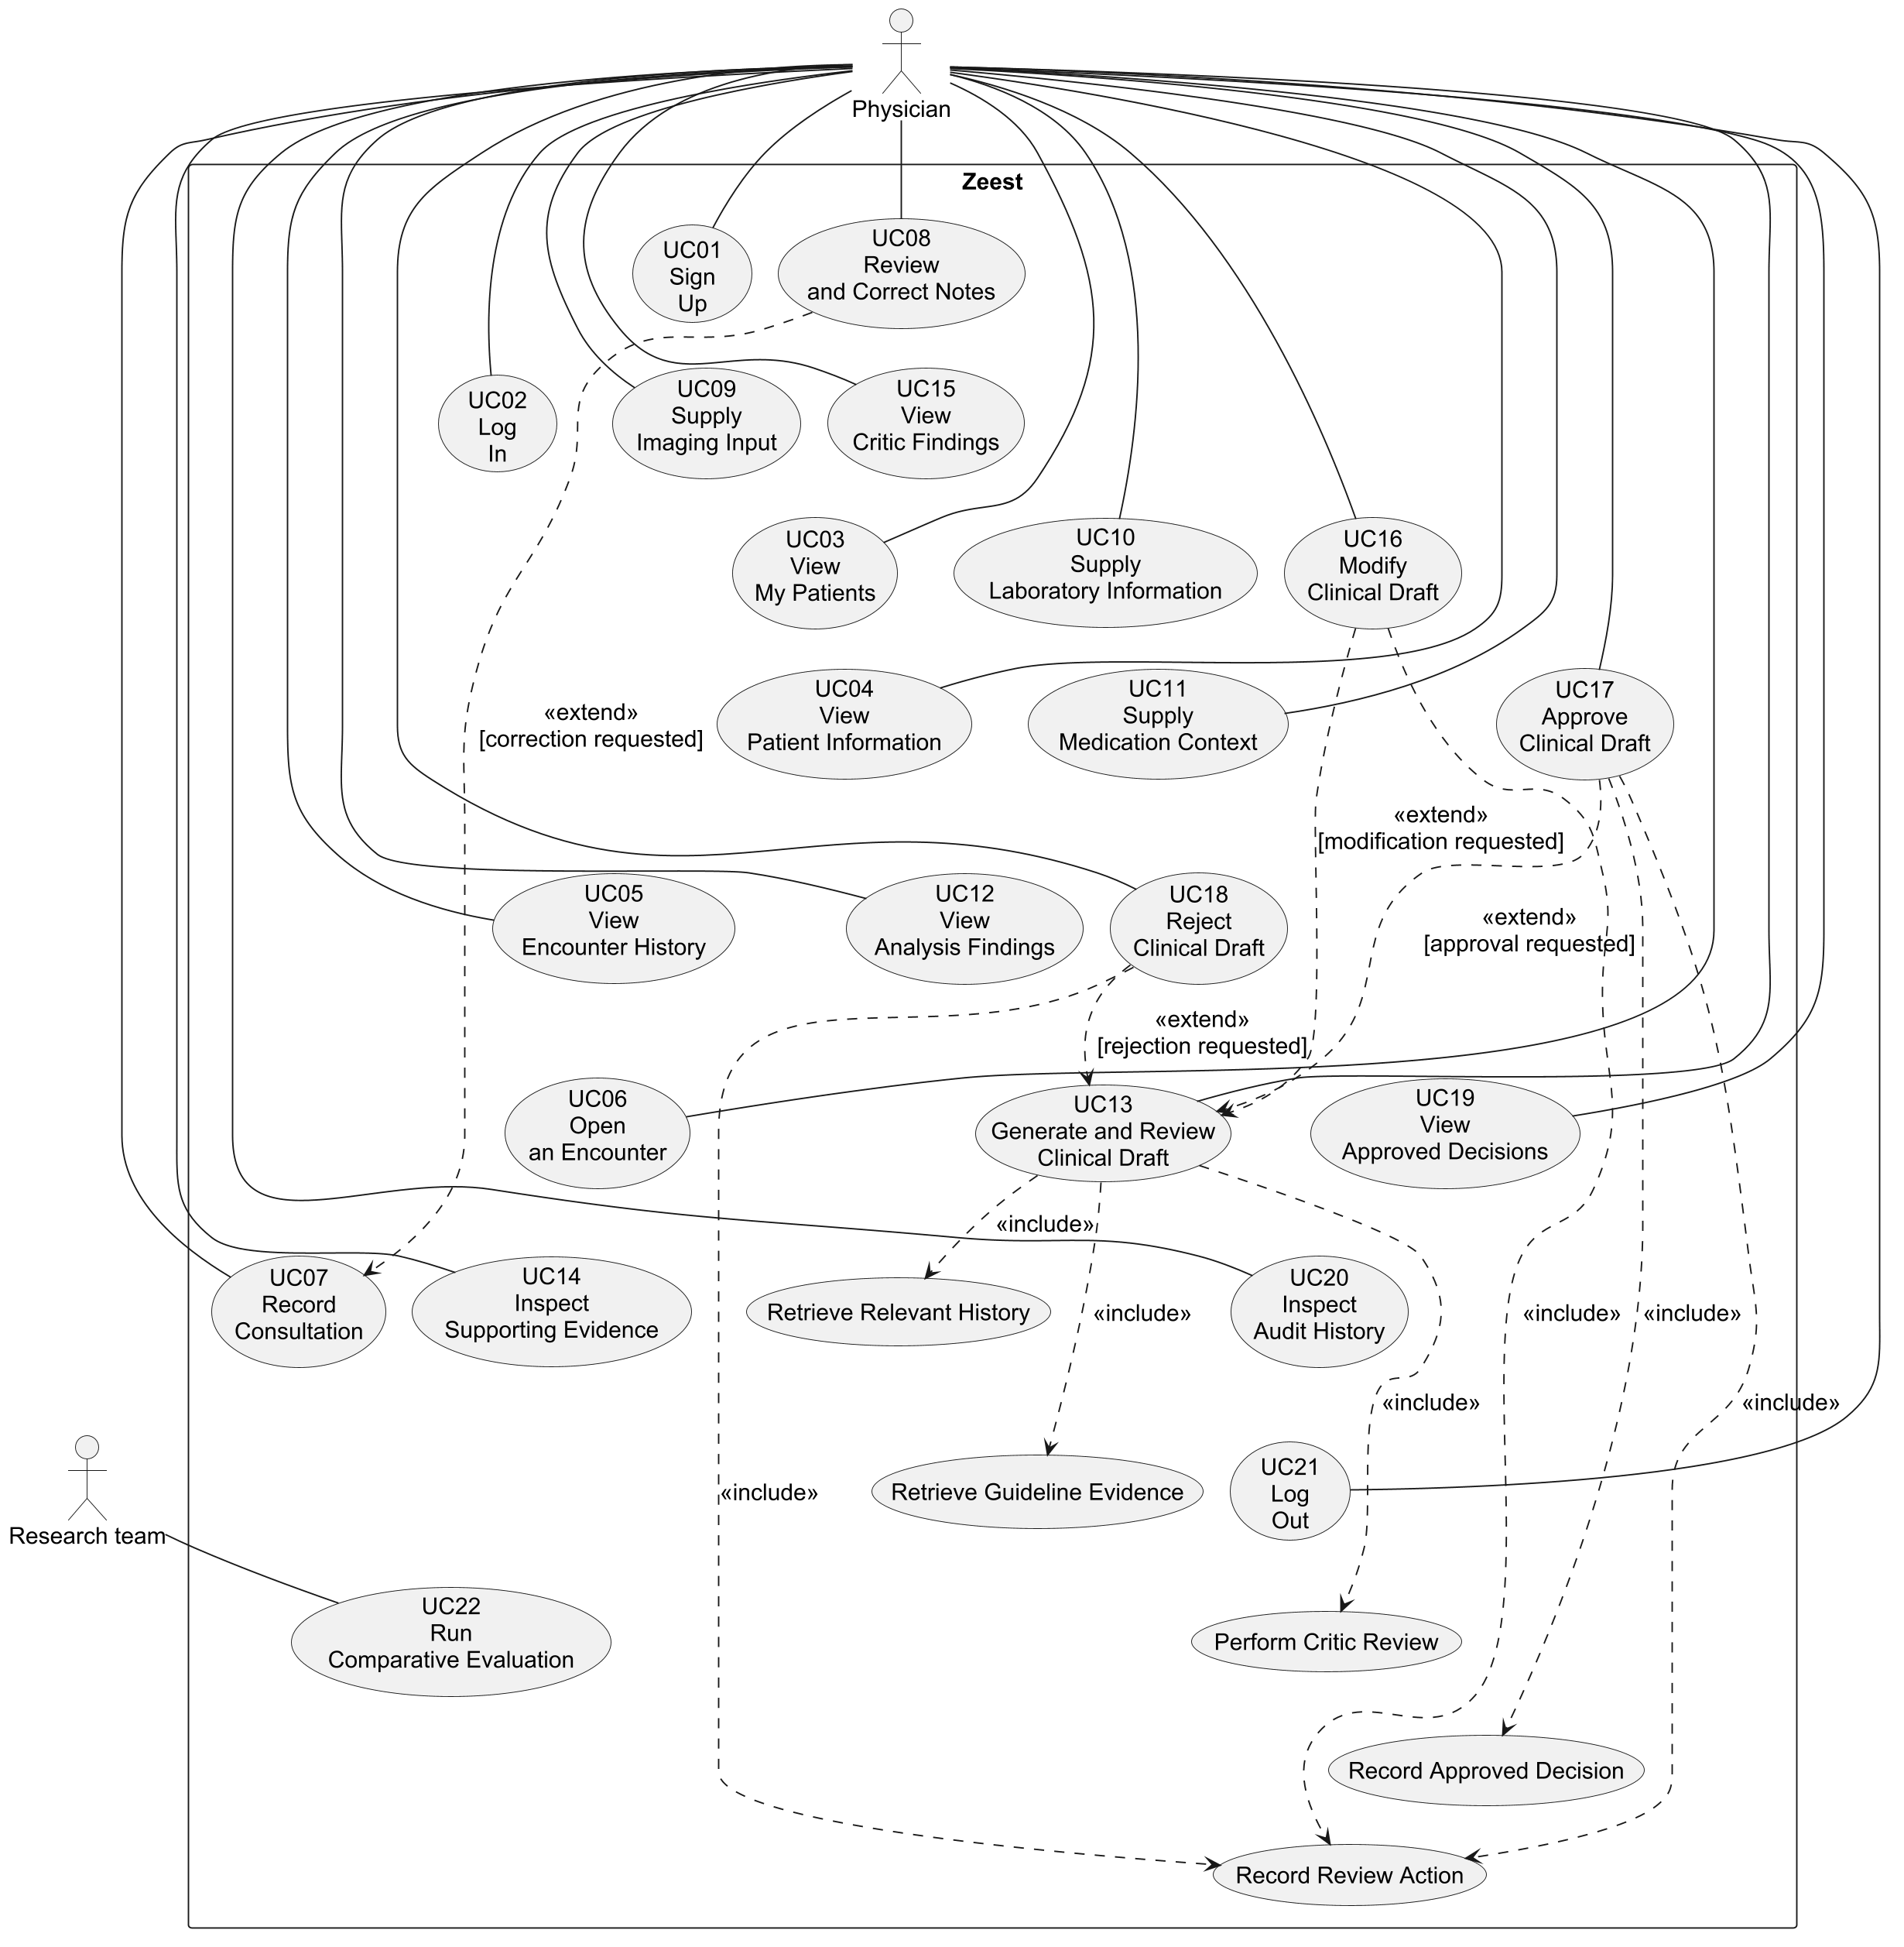
\includegraphics[width=0.96\textwidth,height=0.78\textheight,keepaspectratio]{Figures/kashaf_D01_doctor_use_cases.png}
\caption{Zeest use cases inside one system boundary, with Physician and Research team actors outside. Dashed arrows distinguish mandatory included processing from conditional review actions.}
\label{fig:kashaf:usecases}
\end{figure}

\begin{reporttable}
\centering
\small
\caption{UC01: Sign Up.}
\label{tab:kashaf:uc01}
\begin{tabular}{|p{0.035\textwidth}|p{0.19\textwidth}|p{0.18\textwidth}|p{0.035\textwidth}|p{0.36\textwidth}|}
\hline
\multicolumn{2}{|p{\dimexpr0.225\textwidth+2\tabcolsep+\arrayrulewidth\relax}|}{Name} & \multicolumn{3}{p{\dimexpr0.575\textwidth+4\tabcolsep+2\arrayrulewidth\relax}|}{UC01: Sign Up} \\ \hline
\multicolumn{2}{|p{\dimexpr0.225\textwidth+2\tabcolsep+\arrayrulewidth\relax}|}{Actors} & \multicolumn{3}{p{\dimexpr0.575\textwidth+4\tabcolsep+2\arrayrulewidth\relax}|}{Physician} \\ \hline
\multicolumn{2}{|p{\dimexpr0.225\textwidth+2\tabcolsep+\arrayrulewidth\relax}|}{Summary} & \multicolumn{3}{p{\dimexpr0.575\textwidth+4\tabcolsep+2\arrayrulewidth\relax}|}{The physician creates an account using their registration information.} \\ \hline
\multicolumn{2}{|p{\dimexpr0.225\textwidth+2\tabcolsep+\arrayrulewidth\relax}|}{Pre-Conditions} & \multicolumn{3}{p{\dimexpr0.575\textwidth+4\tabcolsep+2\arrayrulewidth\relax}|}{The physician is not logged in and registration is available.} \\ \hline
\multicolumn{2}{|p{\dimexpr0.225\textwidth+2\tabcolsep+\arrayrulewidth\relax}|}{Post-Conditions} & \multicolumn{3}{p{\dimexpr0.575\textwidth+4\tabcolsep+2\arrayrulewidth\relax}|}{An account is created and the login page is displayed.} \\ \hline
\multicolumn{2}{|p{\dimexpr0.225\textwidth+2\tabcolsep+\arrayrulewidth\relax}|}{Special Requirements} & \multicolumn{3}{p{\dimexpr0.575\textwidth+4\tabcolsep+2\arrayrulewidth\relax}|}{Valid email address; required name and password; securely stored password.} \\ \hline
\multicolumn{5}{|c|}{Basic Flow} \\ \hline
\multicolumn{3}{|c|}{Actor Action} & \multicolumn{2}{c|}{System Response} \\ \hline
1 & \multicolumn{2}{p{\dimexpr0.37\textwidth+2\tabcolsep+\arrayrulewidth\relax}|}{Selects Sign Up.} & 2 & Displays the registration form. \\ \hline
3 & \multicolumn{2}{p{\dimexpr0.37\textwidth+2\tabcolsep+\arrayrulewidth\relax}|}{Enters name, email and password and submits.} & 4 & Validates the information, creates the account and displays Log In. \\ \hline
\multicolumn{5}{|c|}{Alternative Flow} \\ \hline
3 & \multicolumn{2}{p{\dimexpr0.37\textwidth+2\tabcolsep+\arrayrulewidth\relax}|}{Submits incomplete or invalid information.} & 4-A & Identifies the invalid or missing fields without creating an account. \\ \hline
3 & \multicolumn{2}{p{\dimexpr0.37\textwidth+2\tabcolsep+\arrayrulewidth\relax}|}{Uses an email already registered.} & 4-B & Explains that the email is already registered without creating another account. \\ \hline
\end{tabular}
\end{reporttable}

\begin{reporttable}
\centering
\small
\caption{UC02: Log In.}
\label{tab:kashaf:uc02}
\begin{tabular}{|p{0.035\textwidth}|p{0.19\textwidth}|p{0.18\textwidth}|p{0.035\textwidth}|p{0.36\textwidth}|}
\hline
\multicolumn{2}{|p{\dimexpr0.225\textwidth+2\tabcolsep+\arrayrulewidth\relax}|}{Name} & \multicolumn{3}{p{\dimexpr0.575\textwidth+4\tabcolsep+2\arrayrulewidth\relax}|}{UC02: Log In} \\ \hline
\multicolumn{2}{|p{\dimexpr0.225\textwidth+2\tabcolsep+\arrayrulewidth\relax}|}{Actors} & \multicolumn{3}{p{\dimexpr0.575\textwidth+4\tabcolsep+2\arrayrulewidth\relax}|}{Physician} \\ \hline
\multicolumn{2}{|p{\dimexpr0.225\textwidth+2\tabcolsep+\arrayrulewidth\relax}|}{Summary} & \multicolumn{3}{p{\dimexpr0.575\textwidth+4\tabcolsep+2\arrayrulewidth\relax}|}{The physician accesses their account and patient records.} \\ \hline
\multicolumn{2}{|p{\dimexpr0.225\textwidth+2\tabcolsep+\arrayrulewidth\relax}|}{Pre-Conditions} & \multicolumn{3}{p{\dimexpr0.575\textwidth+4\tabcolsep+2\arrayrulewidth\relax}|}{The physician has a registered account and is not logged in.} \\ \hline
\multicolumn{2}{|p{\dimexpr0.225\textwidth+2\tabcolsep+\arrayrulewidth\relax}|}{Post-Conditions} & \multicolumn{3}{p{\dimexpr0.575\textwidth+4\tabcolsep+2\arrayrulewidth\relax}|}{An authenticated session is established.} \\ \hline
\multicolumn{2}{|p{\dimexpr0.225\textwidth+2\tabcolsep+\arrayrulewidth\relax}|}{Special Requirements} & \multicolumn{3}{p{\dimexpr0.575\textwidth+4\tabcolsep+2\arrayrulewidth\relax}|}{Valid registered email and password.} \\ \hline
\multicolumn{5}{|c|}{Basic Flow} \\ \hline
\multicolumn{3}{|c|}{Actor Action} & \multicolumn{2}{c|}{System Response} \\ \hline
1 & \multicolumn{2}{p{\dimexpr0.37\textwidth+2\tabcolsep+\arrayrulewidth\relax}|}{Selects Log In.} & 2 & Displays the login form. \\ \hline
3 & \multicolumn{2}{p{\dimexpr0.37\textwidth+2\tabcolsep+\arrayrulewidth\relax}|}{Enters email and password and submits.} & 4 & Authenticates the account and opens its patient list. \\ \hline
\multicolumn{5}{|c|}{Alternative Flow} \\ \hline
3 & \multicolumn{2}{p{\dimexpr0.37\textwidth+2\tabcolsep+\arrayrulewidth\relax}|}{Enters invalid credentials.} & 4-A & Displays an invalid-credentials message without establishing a session. \\ \hline
\end{tabular}
\end{reporttable}

\begin{reporttable}
\centering
\small
\caption{UC03: View My Patients.}
\label{tab:kashaf:uc03}
\begin{tabular}{|p{0.035\textwidth}|p{0.19\textwidth}|p{0.18\textwidth}|p{0.035\textwidth}|p{0.36\textwidth}|}
\hline
\multicolumn{2}{|p{\dimexpr0.225\textwidth+2\tabcolsep+\arrayrulewidth\relax}|}{Name} & \multicolumn{3}{p{\dimexpr0.575\textwidth+4\tabcolsep+2\arrayrulewidth\relax}|}{UC03: View My Patients} \\ \hline
\multicolumn{2}{|p{\dimexpr0.225\textwidth+2\tabcolsep+\arrayrulewidth\relax}|}{Actors} & \multicolumn{3}{p{\dimexpr0.575\textwidth+4\tabcolsep+2\arrayrulewidth\relax}|}{Physician} \\ \hline
\multicolumn{2}{|p{\dimexpr0.225\textwidth+2\tabcolsep+\arrayrulewidth\relax}|}{Summary} & \multicolumn{3}{p{\dimexpr0.575\textwidth+4\tabcolsep+2\arrayrulewidth\relax}|}{The physician views and selects from their patient records.} \\ \hline
\multicolumn{2}{|p{\dimexpr0.225\textwidth+2\tabcolsep+\arrayrulewidth\relax}|}{Pre-Conditions} & \multicolumn{3}{p{\dimexpr0.575\textwidth+4\tabcolsep+2\arrayrulewidth\relax}|}{The physician is logged in.} \\ \hline
\multicolumn{2}{|p{\dimexpr0.225\textwidth+2\tabcolsep+\arrayrulewidth\relax}|}{Post-Conditions} & \multicolumn{3}{p{\dimexpr0.575\textwidth+4\tabcolsep+2\arrayrulewidth\relax}|}{The physician's patient list is displayed.} \\ \hline
\multicolumn{2}{|p{\dimexpr0.225\textwidth+2\tabcolsep+\arrayrulewidth\relax}|}{Special Requirements} & \multicolumn{3}{p{\dimexpr0.575\textwidth+4\tabcolsep+2\arrayrulewidth\relax}|}{Only records belonging to the logged-in physician are accessible.} \\ \hline
\multicolumn{5}{|c|}{Basic Flow} \\ \hline
\multicolumn{3}{|c|}{Actor Action} & \multicolumn{2}{c|}{System Response} \\ \hline
1 & \multicolumn{2}{p{\dimexpr0.37\textwidth+2\tabcolsep+\arrayrulewidth\relax}|}{Opens My Patients.} & 2 & Retrieves and displays only the physician's patient records. \\ \hline
3 & \multicolumn{2}{p{\dimexpr0.37\textwidth+2\tabcolsep+\arrayrulewidth\relax}|}{Selects a patient.} & 4 & Retains the selected patient and provides access to their information. \\ \hline
\multicolumn{5}{|c|}{Alternative Flow} \\ \hline
1 & \multicolumn{2}{p{\dimexpr0.37\textwidth+2\tabcolsep+\arrayrulewidth\relax}|}{Opens a list without assigned patients.} & 2-A & Displays an empty patient-list message. \\ \hline
\end{tabular}
\end{reporttable}

\begin{reporttable}
\centering
\small
\caption{UC04: View Patient Information.}
\label{tab:kashaf:uc04}
\begin{tabular}{|p{0.035\textwidth}|p{0.19\textwidth}|p{0.18\textwidth}|p{0.035\textwidth}|p{0.36\textwidth}|}
\hline
\multicolumn{2}{|p{\dimexpr0.225\textwidth+2\tabcolsep+\arrayrulewidth\relax}|}{Name} & \multicolumn{3}{p{\dimexpr0.575\textwidth+4\tabcolsep+2\arrayrulewidth\relax}|}{UC04: View Patient Information} \\ \hline
\multicolumn{2}{|p{\dimexpr0.225\textwidth+2\tabcolsep+\arrayrulewidth\relax}|}{Actors} & \multicolumn{3}{p{\dimexpr0.575\textwidth+4\tabcolsep+2\arrayrulewidth\relax}|}{Physician} \\ \hline
\multicolumn{2}{|p{\dimexpr0.225\textwidth+2\tabcolsep+\arrayrulewidth\relax}|}{Summary} & \multicolumn{3}{p{\dimexpr0.575\textwidth+4\tabcolsep+2\arrayrulewidth\relax}|}{The physician reviews the selected patient's available information.} \\ \hline
\multicolumn{2}{|p{\dimexpr0.225\textwidth+2\tabcolsep+\arrayrulewidth\relax}|}{Pre-Conditions} & \multicolumn{3}{p{\dimexpr0.575\textwidth+4\tabcolsep+2\arrayrulewidth\relax}|}{The physician is logged in and one of their own patients is selected.} \\ \hline
\multicolumn{2}{|p{\dimexpr0.225\textwidth+2\tabcolsep+\arrayrulewidth\relax}|}{Post-Conditions} & \multicolumn{3}{p{\dimexpr0.575\textwidth+4\tabcolsep+2\arrayrulewidth\relax}|}{Patient information is displayed.} \\ \hline
\multicolumn{2}{|p{\dimexpr0.225\textwidth+2\tabcolsep+\arrayrulewidth\relax}|}{Special Requirements} & \multicolumn{3}{p{\dimexpr0.575\textwidth+4\tabcolsep+2\arrayrulewidth\relax}|}{Physician ownership must be checked before displaying the record.} \\ \hline
\multicolumn{5}{|c|}{Basic Flow} \\ \hline
\multicolumn{3}{|c|}{Actor Action} & \multicolumn{2}{c|}{System Response} \\ \hline
1 & \multicolumn{2}{p{\dimexpr0.37\textwidth+2\tabcolsep+\arrayrulewidth\relax}|}{Opens the selected patient.} & 2 & Checks ownership and displays patient information. \\ \hline
3 & \multicolumn{2}{p{\dimexpr0.37\textwidth+2\tabcolsep+\arrayrulewidth\relax}|}{Reviews the information.} & 4 & Keeps the selected patient context for subsequent actions. \\ \hline
\multicolumn{5}{|c|}{Alternative Flow} \\ \hline
1 & \multicolumn{2}{p{\dimexpr0.37\textwidth+2\tabcolsep+\arrayrulewidth\relax}|}{Requests another physician's patient record.} & 2-A & Denies access without displaying the record. \\ \hline
\end{tabular}
\end{reporttable}

\begin{reporttable}
\centering
\small
\caption{UC05: View Encounter History.}
\label{tab:kashaf:uc05}
\begin{tabular}{|p{0.035\textwidth}|p{0.19\textwidth}|p{0.18\textwidth}|p{0.035\textwidth}|p{0.36\textwidth}|}
\hline
\multicolumn{2}{|p{\dimexpr0.225\textwidth+2\tabcolsep+\arrayrulewidth\relax}|}{Name} & \multicolumn{3}{p{\dimexpr0.575\textwidth+4\tabcolsep+2\arrayrulewidth\relax}|}{UC05: View Encounter History} \\ \hline
\multicolumn{2}{|p{\dimexpr0.225\textwidth+2\tabcolsep+\arrayrulewidth\relax}|}{Actors} & \multicolumn{3}{p{\dimexpr0.575\textwidth+4\tabcolsep+2\arrayrulewidth\relax}|}{Physician} \\ \hline
\multicolumn{2}{|p{\dimexpr0.225\textwidth+2\tabcolsep+\arrayrulewidth\relax}|}{Summary} & \multicolumn{3}{p{\dimexpr0.575\textwidth+4\tabcolsep+2\arrayrulewidth\relax}|}{The physician reviews the selected patient's previous encounters.} \\ \hline
\multicolumn{2}{|p{\dimexpr0.225\textwidth+2\tabcolsep+\arrayrulewidth\relax}|}{Pre-Conditions} & \multicolumn{3}{p{\dimexpr0.575\textwidth+4\tabcolsep+2\arrayrulewidth\relax}|}{The physician is logged in and one of their own patients is selected.} \\ \hline
\multicolumn{2}{|p{\dimexpr0.225\textwidth+2\tabcolsep+\arrayrulewidth\relax}|}{Post-Conditions} & \multicolumn{3}{p{\dimexpr0.575\textwidth+4\tabcolsep+2\arrayrulewidth\relax}|}{Historical encounter information is displayed.} \\ \hline
\multicolumn{2}{|p{\dimexpr0.225\textwidth+2\tabcolsep+\arrayrulewidth\relax}|}{Special Requirements} & \multicolumn{3}{p{\dimexpr0.575\textwidth+4\tabcolsep+2\arrayrulewidth\relax}|}{History must retain its patient, encounter and source relationships.} \\ \hline
\multicolumn{5}{|c|}{Basic Flow} \\ \hline
\multicolumn{3}{|c|}{Actor Action} & \multicolumn{2}{c|}{System Response} \\ \hline
1 & \multicolumn{2}{p{\dimexpr0.37\textwidth+2\tabcolsep+\arrayrulewidth\relax}|}{Selects Encounter History.} & 2 & Displays the patient's previous encounters. \\ \hline
3 & \multicolumn{2}{p{\dimexpr0.37\textwidth+2\tabcolsep+\arrayrulewidth\relax}|}{Selects a previous encounter.} & 4 & Displays available notes and clinical information with their sources. \\ \hline
\multicolumn{5}{|c|}{Alternative Flow} \\ \hline
1 & \multicolumn{2}{p{\dimexpr0.37\textwidth+2\tabcolsep+\arrayrulewidth\relax}|}{Opens history with no previous encounters.} & 2-A & Displays an empty-history message. \\ \hline
\end{tabular}
\end{reporttable}

\begin{reporttable}
\centering
\small
\caption{UC06: Open an Encounter.}
\label{tab:kashaf:uc06}
\begin{tabular}{|p{0.035\textwidth}|p{0.19\textwidth}|p{0.18\textwidth}|p{0.035\textwidth}|p{0.36\textwidth}|}
\hline
\multicolumn{2}{|p{\dimexpr0.225\textwidth+2\tabcolsep+\arrayrulewidth\relax}|}{Name} & \multicolumn{3}{p{\dimexpr0.575\textwidth+4\tabcolsep+2\arrayrulewidth\relax}|}{UC06: Open an Encounter} \\ \hline
\multicolumn{2}{|p{\dimexpr0.225\textwidth+2\tabcolsep+\arrayrulewidth\relax}|}{Actors} & \multicolumn{3}{p{\dimexpr0.575\textwidth+4\tabcolsep+2\arrayrulewidth\relax}|}{Physician} \\ \hline
\multicolumn{2}{|p{\dimexpr0.225\textwidth+2\tabcolsep+\arrayrulewidth\relax}|}{Summary} & \multicolumn{3}{p{\dimexpr0.575\textwidth+4\tabcolsep+2\arrayrulewidth\relax}|}{The physician opens the encounter used for consultation and review.} \\ \hline
\multicolumn{2}{|p{\dimexpr0.225\textwidth+2\tabcolsep+\arrayrulewidth\relax}|}{Pre-Conditions} & \multicolumn{3}{p{\dimexpr0.575\textwidth+4\tabcolsep+2\arrayrulewidth\relax}|}{The physician is logged in and one of their own patients is selected. An encounter record exists.} \\ \hline
\multicolumn{2}{|p{\dimexpr0.225\textwidth+2\tabcolsep+\arrayrulewidth\relax}|}{Post-Conditions} & \multicolumn{3}{p{\dimexpr0.575\textwidth+4\tabcolsep+2\arrayrulewidth\relax}|}{The encounter becomes the context for clinical actions.} \\ \hline
\multicolumn{2}{|p{\dimexpr0.225\textwidth+2\tabcolsep+\arrayrulewidth\relax}|}{Special Requirements} & \multicolumn{3}{p{\dimexpr0.575\textwidth+4\tabcolsep+2\arrayrulewidth\relax}|}{The encounter must belong to the selected patient and physician.} \\ \hline
\multicolumn{5}{|c|}{Basic Flow} \\ \hline
\multicolumn{3}{|c|}{Actor Action} & \multicolumn{2}{c|}{System Response} \\ \hline
1 & \multicolumn{2}{p{\dimexpr0.37\textwidth+2\tabcolsep+\arrayrulewidth\relax}|}{Selects an encounter.} & 2 & Checks its patient and physician associations. \\ \hline
3 & \multicolumn{2}{p{\dimexpr0.37\textwidth+2\tabcolsep+\arrayrulewidth\relax}|}{Opens the encounter.} & 4 & Displays its consultation workspace and existing inputs. \\ \hline
\multicolumn{5}{|c|}{Alternative Flow} \\ \hline
1 & \multicolumn{2}{p{\dimexpr0.37\textwidth+2\tabcolsep+\arrayrulewidth\relax}|}{Selects an unavailable or unauthorised encounter.} & 2-A & Rejects the selection without exposing its information. \\ \hline
\end{tabular}
\end{reporttable}

\begin{reporttable}
\centering
\small
\caption{UC07: Record Consultation.}
\label{tab:kashaf:uc07}
\begin{tabular}{|p{0.035\textwidth}|p{0.19\textwidth}|p{0.18\textwidth}|p{0.035\textwidth}|p{0.36\textwidth}|}
\hline
\multicolumn{2}{|p{\dimexpr0.225\textwidth+2\tabcolsep+\arrayrulewidth\relax}|}{Name} & \multicolumn{3}{p{\dimexpr0.575\textwidth+4\tabcolsep+2\arrayrulewidth\relax}|}{UC07: Record Consultation} \\ \hline
\multicolumn{2}{|p{\dimexpr0.225\textwidth+2\tabcolsep+\arrayrulewidth\relax}|}{Actors} & \multicolumn{3}{p{\dimexpr0.575\textwidth+4\tabcolsep+2\arrayrulewidth\relax}|}{Physician} \\ \hline
\multicolumn{2}{|p{\dimexpr0.225\textwidth+2\tabcolsep+\arrayrulewidth\relax}|}{Summary} & \multicolumn{3}{p{\dimexpr0.575\textwidth+4\tabcolsep+2\arrayrulewidth\relax}|}{The physician captures audio and obtains structured consultation notes.} \\ \hline
\multicolumn{2}{|p{\dimexpr0.225\textwidth+2\tabcolsep+\arrayrulewidth\relax}|}{Pre-Conditions} & \multicolumn{3}{p{\dimexpr0.575\textwidth+4\tabcolsep+2\arrayrulewidth\relax}|}{The physician is logged in and an encounter for one of their own patients is open.} \\ \hline
\multicolumn{2}{|p{\dimexpr0.225\textwidth+2\tabcolsep+\arrayrulewidth\relax}|}{Post-Conditions} & \multicolumn{3}{p{\dimexpr0.575\textwidth+4\tabcolsep+2\arrayrulewidth\relax}|}{Captured consultation content is presented as structured notes.} \\ \hline
\multicolumn{2}{|p{\dimexpr0.225\textwidth+2\tabcolsep+\arrayrulewidth\relax}|}{Special Requirements} & \multicolumn{3}{p{\dimexpr0.575\textwidth+4\tabcolsep+2\arrayrulewidth\relax}|}{Working microphone, recording permission and supported transcription service.} \\ \hline
\multicolumn{5}{|c|}{Basic Flow} \\ \hline
\multicolumn{3}{|c|}{Actor Action} & \multicolumn{2}{c|}{System Response} \\ \hline
1 & \multicolumn{2}{p{\dimexpr0.37\textwidth+2\tabcolsep+\arrayrulewidth\relax}|}{Selects Start Recording.} & 2 & Checks audio access and begins capture and transcription. \\ \hline
3 & \multicolumn{2}{p{\dimexpr0.37\textwidth+2\tabcolsep+\arrayrulewidth\relax}|}{Conducts the consultation.} & 4 & Transcribes incoming audio into structured notes. \\ \hline
5 & \multicolumn{2}{p{\dimexpr0.37\textwidth+2\tabcolsep+\arrayrulewidth\relax}|}{Selects Stop Recording.} & 6 & Stops capture and presents the resulting notes. \\ \hline
\multicolumn{5}{|c|}{Alternative Flow} \\ \hline
1 & \multicolumn{2}{p{\dimexpr0.37\textwidth+2\tabcolsep+\arrayrulewidth\relax}|}{Cannot grant microphone permission.} & 2-A & Reports the access problem without recording. \\ \hline
3 & \multicolumn{2}{p{\dimexpr0.37\textwidth+2\tabcolsep+\arrayrulewidth\relax}|}{Continues when transcription fails.} & 4-A & Reports the failure and identifies incomplete notes. \\ \hline
\end{tabular}
\end{reporttable}

\begin{reporttable}
\centering
\small
\caption{UC08: Review and Correct Notes.}
\label{tab:kashaf:uc08}
\begin{tabular}{|p{0.035\textwidth}|p{0.19\textwidth}|p{0.18\textwidth}|p{0.035\textwidth}|p{0.36\textwidth}|}
\hline
\multicolumn{2}{|p{\dimexpr0.225\textwidth+2\tabcolsep+\arrayrulewidth\relax}|}{Name} & \multicolumn{3}{p{\dimexpr0.575\textwidth+4\tabcolsep+2\arrayrulewidth\relax}|}{UC08: Review and Correct Notes} \\ \hline
\multicolumn{2}{|p{\dimexpr0.225\textwidth+2\tabcolsep+\arrayrulewidth\relax}|}{Actors} & \multicolumn{3}{p{\dimexpr0.575\textwidth+4\tabcolsep+2\arrayrulewidth\relax}|}{Physician} \\ \hline
\multicolumn{2}{|p{\dimexpr0.225\textwidth+2\tabcolsep+\arrayrulewidth\relax}|}{Summary} & \multicolumn{3}{p{\dimexpr0.575\textwidth+4\tabcolsep+2\arrayrulewidth\relax}|}{The physician reviews and saves corrections to consultation notes.} \\ \hline
\multicolumn{2}{|p{\dimexpr0.225\textwidth+2\tabcolsep+\arrayrulewidth\relax}|}{Pre-Conditions} & \multicolumn{3}{p{\dimexpr0.575\textwidth+4\tabcolsep+2\arrayrulewidth\relax}|}{The physician is logged in and an encounter for one of their own patients is open. Structured notes are available.} \\ \hline
\multicolumn{2}{|p{\dimexpr0.225\textwidth+2\tabcolsep+\arrayrulewidth\relax}|}{Post-Conditions} & \multicolumn{3}{p{\dimexpr0.575\textwidth+4\tabcolsep+2\arrayrulewidth\relax}|}{The reviewed notes are retained for the encounter.} \\ \hline
\multicolumn{2}{|p{\dimexpr0.225\textwidth+2\tabcolsep+\arrayrulewidth\relax}|}{Special Requirements} & \multicolumn{3}{p{\dimexpr0.575\textwidth+4\tabcolsep+2\arrayrulewidth\relax}|}{Corrections must preserve the encounter association.} \\ \hline
\multicolumn{5}{|c|}{Basic Flow} \\ \hline
\multicolumn{3}{|c|}{Actor Action} & \multicolumn{2}{c|}{System Response} \\ \hline
1 & \multicolumn{2}{p{\dimexpr0.37\textwidth+2\tabcolsep+\arrayrulewidth\relax}|}{Opens the notes.} & 2 & Displays the available structured notes. \\ \hline
3 & \multicolumn{2}{p{\dimexpr0.37\textwidth+2\tabcolsep+\arrayrulewidth\relax}|}{Edits the notes and selects Save.} & 4 & Validates and saves the corrected content. \\ \hline
\multicolumn{5}{|c|}{Alternative Flow} \\ \hline
3 & \multicolumn{2}{p{\dimexpr0.37\textwidth+2\tabcolsep+\arrayrulewidth\relax}|}{Submits unusable note content.} & 4-A & Requests correction and retains the prior saved content. \\ \hline
\end{tabular}
\end{reporttable}

\begin{reporttable}
\centering
\small
\caption{UC09: Supply Imaging Input.}
\label{tab:kashaf:uc09}
\begin{tabular}{|p{0.035\textwidth}|p{0.19\textwidth}|p{0.18\textwidth}|p{0.035\textwidth}|p{0.36\textwidth}|}
\hline
\multicolumn{2}{|p{\dimexpr0.225\textwidth+2\tabcolsep+\arrayrulewidth\relax}|}{Name} & \multicolumn{3}{p{\dimexpr0.575\textwidth+4\tabcolsep+2\arrayrulewidth\relax}|}{UC09: Supply Imaging Input} \\ \hline
\multicolumn{2}{|p{\dimexpr0.225\textwidth+2\tabcolsep+\arrayrulewidth\relax}|}{Actors} & \multicolumn{3}{p{\dimexpr0.575\textwidth+4\tabcolsep+2\arrayrulewidth\relax}|}{Physician} \\ \hline
\multicolumn{2}{|p{\dimexpr0.225\textwidth+2\tabcolsep+\arrayrulewidth\relax}|}{Summary} & \multicolumn{3}{p{\dimexpr0.575\textwidth+4\tabcolsep+2\arrayrulewidth\relax}|}{The physician supplies imaging information for the selected encounter.} \\ \hline
\multicolumn{2}{|p{\dimexpr0.225\textwidth+2\tabcolsep+\arrayrulewidth\relax}|}{Pre-Conditions} & \multicolumn{3}{p{\dimexpr0.575\textwidth+4\tabcolsep+2\arrayrulewidth\relax}|}{The physician is logged in and an encounter for one of their own patients is open.} \\ \hline
\multicolumn{2}{|p{\dimexpr0.225\textwidth+2\tabcolsep+\arrayrulewidth\relax}|}{Post-Conditions} & \multicolumn{3}{p{\dimexpr0.575\textwidth+4\tabcolsep+2\arrayrulewidth\relax}|}{The supplied input is retained and submitted to its specialist agent.} \\ \hline
\multicolumn{2}{|p{\dimexpr0.225\textwidth+2\tabcolsep+\arrayrulewidth\relax}|}{Special Requirements} & \multicolumn{3}{p{\dimexpr0.575\textwidth+4\tabcolsep+2\arrayrulewidth\relax}|}{Input must meet the selected imaging model's supported format and task.} \\ \hline
\multicolumn{5}{|c|}{Basic Flow} \\ \hline
\multicolumn{3}{|c|}{Actor Action} & \multicolumn{2}{c|}{System Response} \\ \hline
1 & \multicolumn{2}{p{\dimexpr0.37\textwidth+2\tabcolsep+\arrayrulewidth\relax}|}{Opens the imaging input control.} & 2 & Displays the supported input requirements. \\ \hline
3 & \multicolumn{2}{p{\dimexpr0.37\textwidth+2\tabcolsep+\arrayrulewidth\relax}|}{Provides the input and submits.} & 4 & Validates the input and submits it for specialised processing. \\ \hline
\multicolumn{5}{|c|}{Alternative Flow} \\ \hline
3 & \multicolumn{2}{p{\dimexpr0.37\textwidth+2\tabcolsep+\arrayrulewidth\relax}|}{Submits missing or unsupported input.} & 4-A & Explains the validation problem without treating the input as processed. \\ \hline
\end{tabular}
\end{reporttable}

\begin{reporttable}
\centering
\small
\caption{UC10: Supply Laboratory Information.}
\label{tab:kashaf:uc10}
\begin{tabular}{|p{0.035\textwidth}|p{0.19\textwidth}|p{0.18\textwidth}|p{0.035\textwidth}|p{0.36\textwidth}|}
\hline
\multicolumn{2}{|p{\dimexpr0.225\textwidth+2\tabcolsep+\arrayrulewidth\relax}|}{Name} & \multicolumn{3}{p{\dimexpr0.575\textwidth+4\tabcolsep+2\arrayrulewidth\relax}|}{UC10: Supply Laboratory Information} \\ \hline
\multicolumn{2}{|p{\dimexpr0.225\textwidth+2\tabcolsep+\arrayrulewidth\relax}|}{Actors} & \multicolumn{3}{p{\dimexpr0.575\textwidth+4\tabcolsep+2\arrayrulewidth\relax}|}{Physician} \\ \hline
\multicolumn{2}{|p{\dimexpr0.225\textwidth+2\tabcolsep+\arrayrulewidth\relax}|}{Summary} & \multicolumn{3}{p{\dimexpr0.575\textwidth+4\tabcolsep+2\arrayrulewidth\relax}|}{The physician supplies laboratory information for the selected encounter.} \\ \hline
\multicolumn{2}{|p{\dimexpr0.225\textwidth+2\tabcolsep+\arrayrulewidth\relax}|}{Pre-Conditions} & \multicolumn{3}{p{\dimexpr0.575\textwidth+4\tabcolsep+2\arrayrulewidth\relax}|}{The physician is logged in and an encounter for one of their own patients is open.} \\ \hline
\multicolumn{2}{|p{\dimexpr0.225\textwidth+2\tabcolsep+\arrayrulewidth\relax}|}{Post-Conditions} & \multicolumn{3}{p{\dimexpr0.575\textwidth+4\tabcolsep+2\arrayrulewidth\relax}|}{The supplied input is retained and submitted to its specialist agent.} \\ \hline
\multicolumn{2}{|p{\dimexpr0.225\textwidth+2\tabcolsep+\arrayrulewidth\relax}|}{Special Requirements} & \multicolumn{3}{p{\dimexpr0.575\textwidth+4\tabcolsep+2\arrayrulewidth\relax}|}{Laboratory values must retain their supplied units and source context.} \\ \hline
\multicolumn{5}{|c|}{Basic Flow} \\ \hline
\multicolumn{3}{|c|}{Actor Action} & \multicolumn{2}{c|}{System Response} \\ \hline
1 & \multicolumn{2}{p{\dimexpr0.37\textwidth+2\tabcolsep+\arrayrulewidth\relax}|}{Opens the laboratory input control.} & 2 & Displays the supported input requirements. \\ \hline
3 & \multicolumn{2}{p{\dimexpr0.37\textwidth+2\tabcolsep+\arrayrulewidth\relax}|}{Provides the input and submits.} & 4 & Validates the input and submits it for specialised processing. \\ \hline
\multicolumn{5}{|c|}{Alternative Flow} \\ \hline
3 & \multicolumn{2}{p{\dimexpr0.37\textwidth+2\tabcolsep+\arrayrulewidth\relax}|}{Submits missing or unsupported input.} & 4-A & Explains the validation problem without treating the input as processed. \\ \hline
\end{tabular}
\end{reporttable}

\begin{reporttable}
\centering
\small
\caption{UC11: Supply Medication Context.}
\label{tab:kashaf:uc11}
\begin{tabular}{|p{0.035\textwidth}|p{0.19\textwidth}|p{0.18\textwidth}|p{0.035\textwidth}|p{0.36\textwidth}|}
\hline
\multicolumn{2}{|p{\dimexpr0.225\textwidth+2\tabcolsep+\arrayrulewidth\relax}|}{Name} & \multicolumn{3}{p{\dimexpr0.575\textwidth+4\tabcolsep+2\arrayrulewidth\relax}|}{UC11: Supply Medication Context} \\ \hline
\multicolumn{2}{|p{\dimexpr0.225\textwidth+2\tabcolsep+\arrayrulewidth\relax}|}{Actors} & \multicolumn{3}{p{\dimexpr0.575\textwidth+4\tabcolsep+2\arrayrulewidth\relax}|}{Physician} \\ \hline
\multicolumn{2}{|p{\dimexpr0.225\textwidth+2\tabcolsep+\arrayrulewidth\relax}|}{Summary} & \multicolumn{3}{p{\dimexpr0.575\textwidth+4\tabcolsep+2\arrayrulewidth\relax}|}{The physician supplies medication information for the selected encounter.} \\ \hline
\multicolumn{2}{|p{\dimexpr0.225\textwidth+2\tabcolsep+\arrayrulewidth\relax}|}{Pre-Conditions} & \multicolumn{3}{p{\dimexpr0.575\textwidth+4\tabcolsep+2\arrayrulewidth\relax}|}{The physician is logged in and an encounter for one of their own patients is open.} \\ \hline
\multicolumn{2}{|p{\dimexpr0.225\textwidth+2\tabcolsep+\arrayrulewidth\relax}|}{Post-Conditions} & \multicolumn{3}{p{\dimexpr0.575\textwidth+4\tabcolsep+2\arrayrulewidth\relax}|}{The supplied input is retained and submitted to its specialist agent.} \\ \hline
\multicolumn{2}{|p{\dimexpr0.225\textwidth+2\tabcolsep+\arrayrulewidth\relax}|}{Special Requirements} & \multicolumn{3}{p{\dimexpr0.575\textwidth+4\tabcolsep+2\arrayrulewidth\relax}|}{Medication information must remain linked to the selected patient and encounter.} \\ \hline
\multicolumn{5}{|c|}{Basic Flow} \\ \hline
\multicolumn{3}{|c|}{Actor Action} & \multicolumn{2}{c|}{System Response} \\ \hline
1 & \multicolumn{2}{p{\dimexpr0.37\textwidth+2\tabcolsep+\arrayrulewidth\relax}|}{Opens the medication input control.} & 2 & Displays the supported input requirements. \\ \hline
3 & \multicolumn{2}{p{\dimexpr0.37\textwidth+2\tabcolsep+\arrayrulewidth\relax}|}{Provides the input and submits.} & 4 & Validates the input and submits it for specialised processing. \\ \hline
\multicolumn{5}{|c|}{Alternative Flow} \\ \hline
3 & \multicolumn{2}{p{\dimexpr0.37\textwidth+2\tabcolsep+\arrayrulewidth\relax}|}{Submits missing or unsupported input.} & 4-A & Explains the validation problem without treating the input as processed. \\ \hline
\end{tabular}
\end{reporttable}

\begin{reporttable}
\centering
\small
\caption{UC12: View Analysis Findings.}
\label{tab:kashaf:uc12}
\begin{tabular}{|p{0.035\textwidth}|p{0.19\textwidth}|p{0.18\textwidth}|p{0.035\textwidth}|p{0.36\textwidth}|}
\hline
\multicolumn{2}{|p{\dimexpr0.225\textwidth+2\tabcolsep+\arrayrulewidth\relax}|}{Name} & \multicolumn{3}{p{\dimexpr0.575\textwidth+4\tabcolsep+2\arrayrulewidth\relax}|}{UC12: View Analysis Findings} \\ \hline
\multicolumn{2}{|p{\dimexpr0.225\textwidth+2\tabcolsep+\arrayrulewidth\relax}|}{Actors} & \multicolumn{3}{p{\dimexpr0.575\textwidth+4\tabcolsep+2\arrayrulewidth\relax}|}{Physician} \\ \hline
\multicolumn{2}{|p{\dimexpr0.225\textwidth+2\tabcolsep+\arrayrulewidth\relax}|}{Summary} & \multicolumn{3}{p{\dimexpr0.575\textwidth+4\tabcolsep+2\arrayrulewidth\relax}|}{The physician inspects specialist findings for the encounter.} \\ \hline
\multicolumn{2}{|p{\dimexpr0.225\textwidth+2\tabcolsep+\arrayrulewidth\relax}|}{Pre-Conditions} & \multicolumn{3}{p{\dimexpr0.575\textwidth+4\tabcolsep+2\arrayrulewidth\relax}|}{The physician is logged in and an encounter for one of their own patients is open. Clinical inputs have been submitted.} \\ \hline
\multicolumn{2}{|p{\dimexpr0.225\textwidth+2\tabcolsep+\arrayrulewidth\relax}|}{Post-Conditions} & \multicolumn{3}{p{\dimexpr0.575\textwidth+4\tabcolsep+2\arrayrulewidth\relax}|}{Available findings and processing states are displayed.} \\ \hline
\multicolumn{2}{|p{\dimexpr0.225\textwidth+2\tabcolsep+\arrayrulewidth\relax}|}{Special Requirements} & \multicolumn{3}{p{\dimexpr0.575\textwidth+4\tabcolsep+2\arrayrulewidth\relax}|}{Findings must identify their source; failures must not appear as successful results.} \\ \hline
\multicolumn{5}{|c|}{Basic Flow} \\ \hline
\multicolumn{3}{|c|}{Actor Action} & \multicolumn{2}{c|}{System Response} \\ \hline
1 & \multicolumn{2}{p{\dimexpr0.37\textwidth+2\tabcolsep+\arrayrulewidth\relax}|}{Opens Analysis Findings.} & 2 & Displays imaging, laboratory and medication results with processing states. \\ \hline
3 & \multicolumn{2}{p{\dimexpr0.37\textwidth+2\tabcolsep+\arrayrulewidth\relax}|}{Selects a finding.} & 4 & Displays its source and available analysis information. \\ \hline
\multicolumn{5}{|c|}{Alternative Flow} \\ \hline
1 & \multicolumn{2}{p{\dimexpr0.37\textwidth+2\tabcolsep+\arrayrulewidth\relax}|}{Requests findings while processing is incomplete.} & 2-A & Displays the pending or failed state rather than a completed result. \\ \hline
\end{tabular}
\end{reporttable}

\begin{reporttable}
\centering
\small
\caption{UC13: Generate and Review Clinical Draft.}
\label{tab:kashaf:uc13}
\begin{tabular}{|p{0.035\textwidth}|p{0.19\textwidth}|p{0.18\textwidth}|p{0.035\textwidth}|p{0.36\textwidth}|}
\hline
\multicolumn{2}{|p{\dimexpr0.225\textwidth+2\tabcolsep+\arrayrulewidth\relax}|}{Name} & \multicolumn{3}{p{\dimexpr0.575\textwidth+4\tabcolsep+2\arrayrulewidth\relax}|}{UC13: Generate and Review Clinical Draft} \\ \hline
\multicolumn{2}{|p{\dimexpr0.225\textwidth+2\tabcolsep+\arrayrulewidth\relax}|}{Actors} & \multicolumn{3}{p{\dimexpr0.575\textwidth+4\tabcolsep+2\arrayrulewidth\relax}|}{Physician} \\ \hline
\multicolumn{2}{|p{\dimexpr0.225\textwidth+2\tabcolsep+\arrayrulewidth\relax}|}{Summary} & \multicolumn{3}{p{\dimexpr0.575\textwidth+4\tabcolsep+2\arrayrulewidth\relax}|}{The physician requests a diagnosis and treatment draft for review.} \\ \hline
\multicolumn{2}{|p{\dimexpr0.225\textwidth+2\tabcolsep+\arrayrulewidth\relax}|}{Pre-Conditions} & \multicolumn{3}{p{\dimexpr0.575\textwidth+4\tabcolsep+2\arrayrulewidth\relax}|}{The physician is logged in and an encounter for one of their own patients is open. Case information is available.} \\ \hline
\multicolumn{2}{|p{\dimexpr0.225\textwidth+2\tabcolsep+\arrayrulewidth\relax}|}{Post-Conditions} & \multicolumn{3}{p{\dimexpr0.575\textwidth+4\tabcolsep+2\arrayrulewidth\relax}|}{An evidence-supported draft and critic findings are available for physician review.} \\ \hline
\multicolumn{2}{|p{\dimexpr0.225\textwidth+2\tabcolsep+\arrayrulewidth\relax}|}{Special Requirements} & \multicolumn{3}{p{\dimexpr0.575\textwidth+4\tabcolsep+2\arrayrulewidth\relax}|}{Relevant history, evidence retrieval and critic review precede presentation.} \\ \hline
\multicolumn{5}{|c|}{Basic Flow} \\ \hline
\multicolumn{3}{|c|}{Actor Action} & \multicolumn{2}{c|}{System Response} \\ \hline
1 & \multicolumn{2}{p{\dimexpr0.37\textwidth+2\tabcolsep+\arrayrulewidth\relax}|}{Selects Generate Draft.} & 2 & Prepares the case with inputs, specialist findings and relevant history. \\ \hline
3 & \multicolumn{2}{p{\dimexpr0.37\textwidth+2\tabcolsep+\arrayrulewidth\relax}|}{Waits for the requested draft.} & 4 & Retrieves evidence, generates the draft, performs critic review and presents the output. \\ \hline
5 & \multicolumn{2}{p{\dimexpr0.37\textwidth+2\tabcolsep+\arrayrulewidth\relax}|}{Reviews the presented draft, evidence and critic findings.} & 6 & Keeps the draft pending while the physician chooses a review action. \\ \hline
\multicolumn{5}{|c|}{Alternative Flow} \\ \hline
1 & \multicolumn{2}{p{\dimexpr0.37\textwidth+2\tabcolsep+\arrayrulewidth\relax}|}{Requests generation without usable case information.} & 2-A & Explains the missing inputs. \\ \hline
3 & \multicolumn{2}{p{\dimexpr0.37\textwidth+2\tabcolsep+\arrayrulewidth\relax}|}{Waits during a processing failure.} & 4-A & Reports the failed stage without presenting an unreviewed output as completed. \\ \hline
\end{tabular}
\end{reporttable}

\begin{reporttable}
\centering
\small
\caption{UC14: Inspect Supporting Evidence.}
\label{tab:kashaf:uc14}
\begin{tabular}{|p{0.035\textwidth}|p{0.19\textwidth}|p{0.18\textwidth}|p{0.035\textwidth}|p{0.36\textwidth}|}
\hline
\multicolumn{2}{|p{\dimexpr0.225\textwidth+2\tabcolsep+\arrayrulewidth\relax}|}{Name} & \multicolumn{3}{p{\dimexpr0.575\textwidth+4\tabcolsep+2\arrayrulewidth\relax}|}{UC14: Inspect Supporting Evidence} \\ \hline
\multicolumn{2}{|p{\dimexpr0.225\textwidth+2\tabcolsep+\arrayrulewidth\relax}|}{Actors} & \multicolumn{3}{p{\dimexpr0.575\textwidth+4\tabcolsep+2\arrayrulewidth\relax}|}{Physician} \\ \hline
\multicolumn{2}{|p{\dimexpr0.225\textwidth+2\tabcolsep+\arrayrulewidth\relax}|}{Summary} & \multicolumn{3}{p{\dimexpr0.575\textwidth+4\tabcolsep+2\arrayrulewidth\relax}|}{The physician reviews citations and passages supporting the draft.} \\ \hline
\multicolumn{2}{|p{\dimexpr0.225\textwidth+2\tabcolsep+\arrayrulewidth\relax}|}{Pre-Conditions} & \multicolumn{3}{p{\dimexpr0.575\textwidth+4\tabcolsep+2\arrayrulewidth\relax}|}{The physician is logged in and an encounter for one of their own patients is open. A generated draft is available.} \\ \hline
\multicolumn{2}{|p{\dimexpr0.225\textwidth+2\tabcolsep+\arrayrulewidth\relax}|}{Post-Conditions} & \multicolumn{3}{p{\dimexpr0.575\textwidth+4\tabcolsep+2\arrayrulewidth\relax}|}{Available supporting evidence is displayed.} \\ \hline
\multicolumn{2}{|p{\dimexpr0.225\textwidth+2\tabcolsep+\arrayrulewidth\relax}|}{Special Requirements} & \multicolumn{3}{p{\dimexpr0.575\textwidth+4\tabcolsep+2\arrayrulewidth\relax}|}{Citations and passages must retain their source and draft relationships.} \\ \hline
\multicolumn{5}{|c|}{Basic Flow} \\ \hline
\multicolumn{3}{|c|}{Actor Action} & \multicolumn{2}{c|}{System Response} \\ \hline
1 & \multicolumn{2}{p{\dimexpr0.37\textwidth+2\tabcolsep+\arrayrulewidth\relax}|}{Opens Supporting Evidence.} & 2 & Displays citations and retrieved passages. \\ \hline
3 & \multicolumn{2}{p{\dimexpr0.37\textwidth+2\tabcolsep+\arrayrulewidth\relax}|}{Selects an evidence item.} & 4 & Displays its source reference and supporting content. \\ \hline
\multicolumn{5}{|c|}{Alternative Flow} \\ \hline
1 & \multicolumn{2}{p{\dimexpr0.37\textwidth+2\tabcolsep+\arrayrulewidth\relax}|}{Reviews a draft with missing supporting evidence.} & 2-A & Identifies the missing support without inventing citations. \\ \hline
\end{tabular}
\end{reporttable}

\begin{reporttable}
\centering
\small
\caption{UC15: View Critic Findings.}
\label{tab:kashaf:uc15}
\begin{tabular}{|p{0.035\textwidth}|p{0.19\textwidth}|p{0.18\textwidth}|p{0.035\textwidth}|p{0.36\textwidth}|}
\hline
\multicolumn{2}{|p{\dimexpr0.225\textwidth+2\tabcolsep+\arrayrulewidth\relax}|}{Name} & \multicolumn{3}{p{\dimexpr0.575\textwidth+4\tabcolsep+2\arrayrulewidth\relax}|}{UC15: View Critic Findings} \\ \hline
\multicolumn{2}{|p{\dimexpr0.225\textwidth+2\tabcolsep+\arrayrulewidth\relax}|}{Actors} & \multicolumn{3}{p{\dimexpr0.575\textwidth+4\tabcolsep+2\arrayrulewidth\relax}|}{Physician} \\ \hline
\multicolumn{2}{|p{\dimexpr0.225\textwidth+2\tabcolsep+\arrayrulewidth\relax}|}{Summary} & \multicolumn{3}{p{\dimexpr0.575\textwidth+4\tabcolsep+2\arrayrulewidth\relax}|}{The physician reviews the safety and consistency assessment of the draft.} \\ \hline
\multicolumn{2}{|p{\dimexpr0.225\textwidth+2\tabcolsep+\arrayrulewidth\relax}|}{Pre-Conditions} & \multicolumn{3}{p{\dimexpr0.575\textwidth+4\tabcolsep+2\arrayrulewidth\relax}|}{The physician is logged in and an encounter for one of their own patients is open. A generated draft is available. Critic review has been performed.} \\ \hline
\multicolumn{2}{|p{\dimexpr0.225\textwidth+2\tabcolsep+\arrayrulewidth\relax}|}{Post-Conditions} & \multicolumn{3}{p{\dimexpr0.575\textwidth+4\tabcolsep+2\arrayrulewidth\relax}|}{Critic findings are displayed alongside the draft.} \\ \hline
\multicolumn{2}{|p{\dimexpr0.225\textwidth+2\tabcolsep+\arrayrulewidth\relax}|}{Special Requirements} & \multicolumn{3}{p{\dimexpr0.575\textwidth+4\tabcolsep+2\arrayrulewidth\relax}|}{The review must identify the draft it assessed and retain physician decision authority.} \\ \hline
\multicolumn{5}{|c|}{Basic Flow} \\ \hline
\multicolumn{3}{|c|}{Actor Action} & \multicolumn{2}{c|}{System Response} \\ \hline
1 & \multicolumn{2}{p{\dimexpr0.37\textwidth+2\tabcolsep+\arrayrulewidth\relax}|}{Opens Critic Findings.} & 2 & Displays the available safety and consistency findings. \\ \hline
3 & \multicolumn{2}{p{\dimexpr0.37\textwidth+2\tabcolsep+\arrayrulewidth\relax}|}{Reviews a finding.} & 4 & Keeps the finding associated with its assessed draft. \\ \hline
\multicolumn{5}{|c|}{Alternative Flow} \\ \hline
1 & \multicolumn{2}{p{\dimexpr0.37\textwidth+2\tabcolsep+\arrayrulewidth\relax}|}{Requests an unavailable critic review.} & 2-A & Displays its unavailable state without claiming a successful review. \\ \hline
\end{tabular}
\end{reporttable}

\begin{reporttable}
\centering
\small
\caption{UC16: Modify Clinical Draft.}
\label{tab:kashaf:uc16}
\begin{tabular}{|p{0.035\textwidth}|p{0.19\textwidth}|p{0.18\textwidth}|p{0.035\textwidth}|p{0.36\textwidth}|}
\hline
\multicolumn{2}{|p{\dimexpr0.225\textwidth+2\tabcolsep+\arrayrulewidth\relax}|}{Name} & \multicolumn{3}{p{\dimexpr0.575\textwidth+4\tabcolsep+2\arrayrulewidth\relax}|}{UC16: Modify Clinical Draft} \\ \hline
\multicolumn{2}{|p{\dimexpr0.225\textwidth+2\tabcolsep+\arrayrulewidth\relax}|}{Actors} & \multicolumn{3}{p{\dimexpr0.575\textwidth+4\tabcolsep+2\arrayrulewidth\relax}|}{Physician} \\ \hline
\multicolumn{2}{|p{\dimexpr0.225\textwidth+2\tabcolsep+\arrayrulewidth\relax}|}{Summary} & \multicolumn{3}{p{\dimexpr0.575\textwidth+4\tabcolsep+2\arrayrulewidth\relax}|}{The physician edits and saves a generated clinical draft.} \\ \hline
\multicolumn{2}{|p{\dimexpr0.225\textwidth+2\tabcolsep+\arrayrulewidth\relax}|}{Pre-Conditions} & \multicolumn{3}{p{\dimexpr0.575\textwidth+4\tabcolsep+2\arrayrulewidth\relax}|}{The physician is logged in and an encounter for one of their own patients is open. A generated draft is available. The draft is pending review.} \\ \hline
\multicolumn{2}{|p{\dimexpr0.225\textwidth+2\tabcolsep+\arrayrulewidth\relax}|}{Post-Conditions} & \multicolumn{3}{p{\dimexpr0.575\textwidth+4\tabcolsep+2\arrayrulewidth\relax}|}{A revised draft is saved and remains pending approval.} \\ \hline
\multicolumn{2}{|p{\dimexpr0.225\textwidth+2\tabcolsep+\arrayrulewidth\relax}|}{Special Requirements} & \multicolumn{3}{p{\dimexpr0.575\textwidth+4\tabcolsep+2\arrayrulewidth\relax}|}{Saving a modification must not record an approved decision.} \\ \hline
\multicolumn{5}{|c|}{Basic Flow} \\ \hline
\multicolumn{3}{|c|}{Actor Action} & \multicolumn{2}{c|}{System Response} \\ \hline
1 & \multicolumn{2}{p{\dimexpr0.37\textwidth+2\tabcolsep+\arrayrulewidth\relax}|}{Selects Modify.} & 2 & Displays editable draft content. \\ \hline
3 & \multicolumn{2}{p{\dimexpr0.37\textwidth+2\tabcolsep+\arrayrulewidth\relax}|}{Edits the content and selects Save.} & 4 & Stores the revised draft and modification action without approval. \\ \hline
\multicolumn{5}{|c|}{Alternative Flow} \\ \hline
3 & \multicolumn{2}{p{\dimexpr0.37\textwidth+2\tabcolsep+\arrayrulewidth\relax}|}{Cancels the edit.} & 4-A & Retains the previous saved revision. \\ \hline
\end{tabular}
\end{reporttable}

\begin{reporttable}
\centering
\small
\caption{UC17: Approve Clinical Draft.}
\label{tab:kashaf:uc17}
\begin{tabular}{|p{0.035\textwidth}|p{0.19\textwidth}|p{0.18\textwidth}|p{0.035\textwidth}|p{0.36\textwidth}|}
\hline
\multicolumn{2}{|p{\dimexpr0.225\textwidth+2\tabcolsep+\arrayrulewidth\relax}|}{Name} & \multicolumn{3}{p{\dimexpr0.575\textwidth+4\tabcolsep+2\arrayrulewidth\relax}|}{UC17: Approve Clinical Draft} \\ \hline
\multicolumn{2}{|p{\dimexpr0.225\textwidth+2\tabcolsep+\arrayrulewidth\relax}|}{Actors} & \multicolumn{3}{p{\dimexpr0.575\textwidth+4\tabcolsep+2\arrayrulewidth\relax}|}{Physician} \\ \hline
\multicolumn{2}{|p{\dimexpr0.225\textwidth+2\tabcolsep+\arrayrulewidth\relax}|}{Summary} & \multicolumn{3}{p{\dimexpr0.575\textwidth+4\tabcolsep+2\arrayrulewidth\relax}|}{The physician explicitly accepts the reviewed draft revision.} \\ \hline
\multicolumn{2}{|p{\dimexpr0.225\textwidth+2\tabcolsep+\arrayrulewidth\relax}|}{Pre-Conditions} & \multicolumn{3}{p{\dimexpr0.575\textwidth+4\tabcolsep+2\arrayrulewidth\relax}|}{The physician is logged in and an encounter for one of their own patients is open. A generated draft is available. The displayed revision is pending review.} \\ \hline
\multicolumn{2}{|p{\dimexpr0.225\textwidth+2\tabcolsep+\arrayrulewidth\relax}|}{Post-Conditions} & \multicolumn{3}{p{\dimexpr0.575\textwidth+4\tabcolsep+2\arrayrulewidth\relax}|}{The accepted content is recorded as an approved clinical decision.} \\ \hline
\multicolumn{2}{|p{\dimexpr0.225\textwidth+2\tabcolsep+\arrayrulewidth\relax}|}{Special Requirements} & \multicolumn{3}{p{\dimexpr0.575\textwidth+4\tabcolsep+2\arrayrulewidth\relax}|}{Approval must identify the exact saved revision and responsible physician.} \\ \hline
\multicolumn{5}{|c|}{Basic Flow} \\ \hline
\multicolumn{3}{|c|}{Actor Action} & \multicolumn{2}{c|}{System Response} \\ \hline
1 & \multicolumn{2}{p{\dimexpr0.37\textwidth+2\tabcolsep+\arrayrulewidth\relax}|}{Selects Approve.} & 2 & Displays the revision and content to confirm. \\ \hline
3 & \multicolumn{2}{p{\dimexpr0.37\textwidth+2\tabcolsep+\arrayrulewidth\relax}|}{Confirms approval.} & 4 & Records the accepted decision and corresponding audit action. \\ \hline
\multicolumn{5}{|c|}{Alternative Flow} \\ \hline
3 & \multicolumn{2}{p{\dimexpr0.37\textwidth+2\tabcolsep+\arrayrulewidth\relax}|}{Confirms after the revision has changed.} & 4-A & Requests review of the current saved revision before approval. \\ \hline
3 & \multicolumn{2}{p{\dimexpr0.37\textwidth+2\tabcolsep+\arrayrulewidth\relax}|}{Cancels confirmation.} & 4-B & Leaves the draft pending. \\ \hline
\end{tabular}
\end{reporttable}

\begin{reporttable}
\centering
\small
\caption{UC18: Reject Clinical Draft.}
\label{tab:kashaf:uc18}
\begin{tabular}{|p{0.035\textwidth}|p{0.19\textwidth}|p{0.18\textwidth}|p{0.035\textwidth}|p{0.36\textwidth}|}
\hline
\multicolumn{2}{|p{\dimexpr0.225\textwidth+2\tabcolsep+\arrayrulewidth\relax}|}{Name} & \multicolumn{3}{p{\dimexpr0.575\textwidth+4\tabcolsep+2\arrayrulewidth\relax}|}{UC18: Reject Clinical Draft} \\ \hline
\multicolumn{2}{|p{\dimexpr0.225\textwidth+2\tabcolsep+\arrayrulewidth\relax}|}{Actors} & \multicolumn{3}{p{\dimexpr0.575\textwidth+4\tabcolsep+2\arrayrulewidth\relax}|}{Physician} \\ \hline
\multicolumn{2}{|p{\dimexpr0.225\textwidth+2\tabcolsep+\arrayrulewidth\relax}|}{Summary} & \multicolumn{3}{p{\dimexpr0.575\textwidth+4\tabcolsep+2\arrayrulewidth\relax}|}{The physician rejects a pending clinical draft.} \\ \hline
\multicolumn{2}{|p{\dimexpr0.225\textwidth+2\tabcolsep+\arrayrulewidth\relax}|}{Pre-Conditions} & \multicolumn{3}{p{\dimexpr0.575\textwidth+4\tabcolsep+2\arrayrulewidth\relax}|}{The physician is logged in and an encounter for one of their own patients is open. A generated draft is available. The draft is pending review.} \\ \hline
\multicolumn{2}{|p{\dimexpr0.225\textwidth+2\tabcolsep+\arrayrulewidth\relax}|}{Post-Conditions} & \multicolumn{3}{p{\dimexpr0.575\textwidth+4\tabcolsep+2\arrayrulewidth\relax}|}{The draft is marked rejected and the action is logged.} \\ \hline
\multicolumn{2}{|p{\dimexpr0.225\textwidth+2\tabcolsep+\arrayrulewidth\relax}|}{Special Requirements} & \multicolumn{3}{p{\dimexpr0.575\textwidth+4\tabcolsep+2\arrayrulewidth\relax}|}{Rejected content must not become an approved decision.} \\ \hline
\multicolumn{5}{|c|}{Basic Flow} \\ \hline
\multicolumn{3}{|c|}{Actor Action} & \multicolumn{2}{c|}{System Response} \\ \hline
1 & \multicolumn{2}{p{\dimexpr0.37\textwidth+2\tabcolsep+\arrayrulewidth\relax}|}{Selects Reject.} & 2 & Requests confirmation for the selected draft. \\ \hline
3 & \multicolumn{2}{p{\dimexpr0.37\textwidth+2\tabcolsep+\arrayrulewidth\relax}|}{Confirms rejection.} & 4 & Records rejection and its audit action without recording a clinical decision. \\ \hline
\multicolumn{5}{|c|}{Alternative Flow} \\ \hline
3 & \multicolumn{2}{p{\dimexpr0.37\textwidth+2\tabcolsep+\arrayrulewidth\relax}|}{Cancels rejection.} & 4-A & Leaves the existing draft state unchanged. \\ \hline
\end{tabular}
\end{reporttable}

\begin{reporttable}
\centering
\small
\caption{UC19: View Approved Decisions.}
\label{tab:kashaf:uc19}
\begin{tabular}{|p{0.035\textwidth}|p{0.19\textwidth}|p{0.18\textwidth}|p{0.035\textwidth}|p{0.36\textwidth}|}
\hline
\multicolumn{2}{|p{\dimexpr0.225\textwidth+2\tabcolsep+\arrayrulewidth\relax}|}{Name} & \multicolumn{3}{p{\dimexpr0.575\textwidth+4\tabcolsep+2\arrayrulewidth\relax}|}{UC19: View Approved Decisions} \\ \hline
\multicolumn{2}{|p{\dimexpr0.225\textwidth+2\tabcolsep+\arrayrulewidth\relax}|}{Actors} & \multicolumn{3}{p{\dimexpr0.575\textwidth+4\tabcolsep+2\arrayrulewidth\relax}|}{Physician} \\ \hline
\multicolumn{2}{|p{\dimexpr0.225\textwidth+2\tabcolsep+\arrayrulewidth\relax}|}{Summary} & \multicolumn{3}{p{\dimexpr0.575\textwidth+4\tabcolsep+2\arrayrulewidth\relax}|}{The physician reviews accepted decisions for their selected patient.} \\ \hline
\multicolumn{2}{|p{\dimexpr0.225\textwidth+2\tabcolsep+\arrayrulewidth\relax}|}{Pre-Conditions} & \multicolumn{3}{p{\dimexpr0.575\textwidth+4\tabcolsep+2\arrayrulewidth\relax}|}{The physician is logged in and one of their own patients is selected.} \\ \hline
\multicolumn{2}{|p{\dimexpr0.225\textwidth+2\tabcolsep+\arrayrulewidth\relax}|}{Post-Conditions} & \multicolumn{3}{p{\dimexpr0.575\textwidth+4\tabcolsep+2\arrayrulewidth\relax}|}{Approved decision content and its encounter context are displayed.} \\ \hline
\multicolumn{2}{|p{\dimexpr0.225\textwidth+2\tabcolsep+\arrayrulewidth\relax}|}{Special Requirements} & \multicolumn{3}{p{\dimexpr0.575\textwidth+4\tabcolsep+2\arrayrulewidth\relax}|}{Only explicitly approved decisions belonging to the physician's patient may be displayed.} \\ \hline
\multicolumn{5}{|c|}{Basic Flow} \\ \hline
\multicolumn{3}{|c|}{Actor Action} & \multicolumn{2}{c|}{System Response} \\ \hline
1 & \multicolumn{2}{p{\dimexpr0.37\textwidth+2\tabcolsep+\arrayrulewidth\relax}|}{Opens Approved Decisions.} & 2 & Displays the patient's approved decisions grouped by encounter. \\ \hline
3 & \multicolumn{2}{p{\dimexpr0.37\textwidth+2\tabcolsep+\arrayrulewidth\relax}|}{Selects a decision.} & 4 & Displays accepted content and its approval context. \\ \hline
\multicolumn{5}{|c|}{Alternative Flow} \\ \hline
1 & \multicolumn{2}{p{\dimexpr0.37\textwidth+2\tabcolsep+\arrayrulewidth\relax}|}{Opens a patient with no approved decisions.} & 2-A & Displays an empty approved-decisions message. \\ \hline
\end{tabular}
\end{reporttable}

\begin{reporttable}
\centering
\small
\caption{UC20: Inspect Audit History.}
\label{tab:kashaf:uc20}
\begin{tabular}{|p{0.035\textwidth}|p{0.19\textwidth}|p{0.18\textwidth}|p{0.035\textwidth}|p{0.36\textwidth}|}
\hline
\multicolumn{2}{|p{\dimexpr0.225\textwidth+2\tabcolsep+\arrayrulewidth\relax}|}{Name} & \multicolumn{3}{p{\dimexpr0.575\textwidth+4\tabcolsep+2\arrayrulewidth\relax}|}{UC20: Inspect Audit History} \\ \hline
\multicolumn{2}{|p{\dimexpr0.225\textwidth+2\tabcolsep+\arrayrulewidth\relax}|}{Actors} & \multicolumn{3}{p{\dimexpr0.575\textwidth+4\tabcolsep+2\arrayrulewidth\relax}|}{Physician} \\ \hline
\multicolumn{2}{|p{\dimexpr0.225\textwidth+2\tabcolsep+\arrayrulewidth\relax}|}{Summary} & \multicolumn{3}{p{\dimexpr0.575\textwidth+4\tabcolsep+2\arrayrulewidth\relax}|}{The physician reviews the encounter's recorded decision actions.} \\ \hline
\multicolumn{2}{|p{\dimexpr0.225\textwidth+2\tabcolsep+\arrayrulewidth\relax}|}{Pre-Conditions} & \multicolumn{3}{p{\dimexpr0.575\textwidth+4\tabcolsep+2\arrayrulewidth\relax}|}{The physician is logged in and an encounter for one of their own patients is open.} \\ \hline
\multicolumn{2}{|p{\dimexpr0.225\textwidth+2\tabcolsep+\arrayrulewidth\relax}|}{Post-Conditions} & \multicolumn{3}{p{\dimexpr0.575\textwidth+4\tabcolsep+2\arrayrulewidth\relax}|}{Review actions are displayed without changing them.} \\ \hline
\multicolumn{2}{|p{\dimexpr0.225\textwidth+2\tabcolsep+\arrayrulewidth\relax}|}{Special Requirements} & \multicolumn{3}{p{\dimexpr0.575\textwidth+4\tabcolsep+2\arrayrulewidth\relax}|}{Actions must retain time, physician identity, draft revision and encounter context.} \\ \hline
\multicolumn{5}{|c|}{Basic Flow} \\ \hline
\multicolumn{3}{|c|}{Actor Action} & \multicolumn{2}{c|}{System Response} \\ \hline
1 & \multicolumn{2}{p{\dimexpr0.37\textwidth+2\tabcolsep+\arrayrulewidth\relax}|}{Opens Audit History.} & 2 & Displays recorded review actions. \\ \hline
3 & \multicolumn{2}{p{\dimexpr0.37\textwidth+2\tabcolsep+\arrayrulewidth\relax}|}{Selects an action.} & 4 & Displays its revision and decision context. \\ \hline
\multicolumn{5}{|c|}{Alternative Flow} \\ \hline
1 & \multicolumn{2}{p{\dimexpr0.37\textwidth+2\tabcolsep+\arrayrulewidth\relax}|}{Opens an encounter without review actions.} & 2-A & Displays an empty audit-history message. \\ \hline
\end{tabular}
\end{reporttable}

\begin{reporttable}
\centering
\small
\caption{UC21: Log Out.}
\label{tab:kashaf:uc21}
\begin{tabular}{|p{0.035\textwidth}|p{0.19\textwidth}|p{0.18\textwidth}|p{0.035\textwidth}|p{0.36\textwidth}|}
\hline
\multicolumn{2}{|p{\dimexpr0.225\textwidth+2\tabcolsep+\arrayrulewidth\relax}|}{Name} & \multicolumn{3}{p{\dimexpr0.575\textwidth+4\tabcolsep+2\arrayrulewidth\relax}|}{UC21: Log Out} \\ \hline
\multicolumn{2}{|p{\dimexpr0.225\textwidth+2\tabcolsep+\arrayrulewidth\relax}|}{Actors} & \multicolumn{3}{p{\dimexpr0.575\textwidth+4\tabcolsep+2\arrayrulewidth\relax}|}{Physician} \\ \hline
\multicolumn{2}{|p{\dimexpr0.225\textwidth+2\tabcolsep+\arrayrulewidth\relax}|}{Summary} & \multicolumn{3}{p{\dimexpr0.575\textwidth+4\tabcolsep+2\arrayrulewidth\relax}|}{The physician ends the application session.} \\ \hline
\multicolumn{2}{|p{\dimexpr0.225\textwidth+2\tabcolsep+\arrayrulewidth\relax}|}{Pre-Conditions} & \multicolumn{3}{p{\dimexpr0.575\textwidth+4\tabcolsep+2\arrayrulewidth\relax}|}{The physician is logged in.} \\ \hline
\multicolumn{2}{|p{\dimexpr0.225\textwidth+2\tabcolsep+\arrayrulewidth\relax}|}{Post-Conditions} & \multicolumn{3}{p{\dimexpr0.575\textwidth+4\tabcolsep+2\arrayrulewidth\relax}|}{The session ends and protected records require login.} \\ \hline
\multicolumn{2}{|p{\dimexpr0.225\textwidth+2\tabcolsep+\arrayrulewidth\relax}|}{Special Requirements} & \multicolumn{3}{p{\dimexpr0.575\textwidth+4\tabcolsep+2\arrayrulewidth\relax}|}{Protected patient information must not remain accessible through the ended session.} \\ \hline
\multicolumn{5}{|c|}{Basic Flow} \\ \hline
\multicolumn{3}{|c|}{Actor Action} & \multicolumn{2}{c|}{System Response} \\ \hline
1 & \multicolumn{2}{p{\dimexpr0.37\textwidth+2\tabcolsep+\arrayrulewidth\relax}|}{Selects Log Out.} & 2 & Terminates the session and displays Log In. \\ \hline
\multicolumn{5}{|c|}{Alternative Flow} \\ \hline
1 & \multicolumn{2}{p{\dimexpr0.37\textwidth+2\tabcolsep+\arrayrulewidth\relax}|}{Selects Log Out after the session has expired.} & 2-A & Displays Log In without restoring access. \\ \hline
\end{tabular}
\end{reporttable}

\begin{reporttable}
\centering
\small
\caption{UC22: Run Comparative Evaluation.}
\label{tab:kashaf:uc22}
\begin{tabular}{|p{0.035\textwidth}|p{0.19\textwidth}|p{0.18\textwidth}|p{0.035\textwidth}|p{0.36\textwidth}|}
\hline
\multicolumn{2}{|p{\dimexpr0.225\textwidth+2\tabcolsep+\arrayrulewidth\relax}|}{Name} & \multicolumn{3}{p{\dimexpr0.575\textwidth+4\tabcolsep+2\arrayrulewidth\relax}|}{UC22: Run Comparative Evaluation} \\ \hline
\multicolumn{2}{|p{\dimexpr0.225\textwidth+2\tabcolsep+\arrayrulewidth\relax}|}{Actors} & \multicolumn{3}{p{\dimexpr0.575\textwidth+4\tabcolsep+2\arrayrulewidth\relax}|}{Research team} \\ \hline
\multicolumn{2}{|p{\dimexpr0.225\textwidth+2\tabcolsep+\arrayrulewidth\relax}|}{Summary} & \multicolumn{3}{p{\dimexpr0.575\textwidth+4\tabcolsep+2\arrayrulewidth\relax}|}{The research team compares the defined system variants.} \\ \hline
\multicolumn{2}{|p{\dimexpr0.225\textwidth+2\tabcolsep+\arrayrulewidth\relax}|}{Pre-Conditions} & \multicolumn{3}{p{\dimexpr0.575\textwidth+4\tabcolsep+2\arrayrulewidth\relax}|}{Permitted cases, reference assessments and configurations are available.} \\ \hline
\multicolumn{2}{|p{\dimexpr0.225\textwidth+2\tabcolsep+\arrayrulewidth\relax}|}{Post-Conditions} & \multicolumn{3}{p{\dimexpr0.575\textwidth+4\tabcolsep+2\arrayrulewidth\relax}|}{Outputs are recorded with their cases and configurations for comparison.} \\ \hline
\multicolumn{2}{|p{\dimexpr0.225\textwidth+2\tabcolsep+\arrayrulewidth\relax}|}{Special Requirements} & \multicolumn{3}{p{\dimexpr0.575\textwidth+4\tabcolsep+2\arrayrulewidth\relax}|}{The baseline, memory variant and full system must use consistent assessment conditions.} \\ \hline
\multicolumn{5}{|c|}{Basic Flow} \\ \hline
\multicolumn{3}{|c|}{Actor Action} & \multicolumn{2}{c|}{System Response} \\ \hline
1 & \multicolumn{2}{p{\dimexpr0.37\textwidth+2\tabcolsep+\arrayrulewidth\relax}|}{Selects cases and configurations.} & 2 & Checks the required inputs and comparison settings. \\ \hline
3 & \multicolumn{2}{p{\dimexpr0.37\textwidth+2\tabcolsep+\arrayrulewidth\relax}|}{Starts evaluation.} & 4 & Runs the variants and records outputs and configuration details. \\ \hline
\multicolumn{5}{|c|}{Alternative Flow} \\ \hline
1 & \multicolumn{2}{p{\dimexpr0.37\textwidth+2\tabcolsep+\arrayrulewidth\relax}|}{Selects unavailable cases or incomplete settings.} & 2-A & Identifies missing prerequisites without fabricating results. \\ \hline
\end{tabular}
\end{reporttable}


\section{Hardware and Software Requirements}

Tables~\ref{tab:kashaf:hardware} and~\ref{tab:kashaf:software} identify the supporting resources.

\subsection{Hardware Requirements}

A development computer must support the application services, storage and the tools used to integrate the processing components. The physician interface needs a browser-capable device and an audio input source for consultation capture. Microphone access must be available when the recording workflow is used, and connectivity must support whichever processing services are selected. Storage must retain the permitted case inputs, relational records and associated semantic representations without separating them from their identifying context. Compute and memory requirements depend on the imaging and transcription models, the language-model access arrangement and the size of the case collection. Table~\ref{tab:kashaf:hardware} records these resource needs with the configuration values that remain to be established. Numerical compute, storage and concurrent-user limits must be established for the selected workload rather than assumed from a candidate model. Resource failures should be identifiable during integration checks. No resource specification alone establishes measured capacity for the integrated clinical processing workflow.

\begin{reporttable}
\centering
\small
\caption{Hardware resources supporting the Zeest workflow.}
\label{tab:kashaf:hardware}
\begin{tabular}{|p{0.24\textwidth}|p{0.36\textwidth}|p{0.28\textwidth}|}
\hline
Resource & Purpose & Specification \\ \hline
Development/processing computer & Application services and selected local processing & Processor and RAM: TBD after model selection. \\ \hline
Physician device & Web interface and review actions & Browser-capable device; supported configurations: TBD. \\ \hline
Audio input & Consultation capture & Working audio source and capture permission. \\ \hline
Storage & Clinical inputs, records, audit actions and vectors & Capacity and retention configuration: TBD. \\ \hline
Graphics acceleration & Local inference where required & GPU requirement depends on the selected model. \\ \hline
Connectivity & Access to selected processing and evidence services & Connection requirements depend on service arrangement. \\ \hline
\end{tabular}
\end{reporttable}

% Finish this section's floats before the next heading.

\subsection{Software Requirements}

FastAPI provides the backend integration layer, while Next.js supports the physician-facing web interface. LangGraph and Google ADK are the named orchestration technologies for coordinating the agent responsibilities, with their exact division to be agreed in the detailed design. Gemini supplies the language-model capability used within the reasoning workflow, and PyTorch supports integration of the imaging model. PostgreSQL stores patient, encounter and review information, with pgvector providing the semantic representation layer alongside relational records. A transcription component and clinical knowledge resources the dependencies needed for consultation capture, guideline retrieval and medication review. Table~\ref{tab:kashaf:software} connects these technologies to their responsibilities. Component versions, model identifiers, representations and access conditions must be recorded when the environment is selected. Component versions and permitted resource use must be recorded before comparative runs. Framework choices do not establish completed integration or guaranteed compatibility. Each selected dependency requires a recorded configuration and an identifiable integration failure path.

\begin{reporttable}
\centering
\small
\caption{Software technologies and processing dependencies used in the Zeest design.}
\label{tab:kashaf:software}
\begin{tabular}{|p{0.25\textwidth}|p{0.34\textwidth}|p{0.29\textwidth}|}
\hline
Technology/resource & Responsibility & Configuration \\ \hline
FastAPI & Backend integration and application interfaces & Version and interface contracts: TBD. \\ \hline
Next.js & Physician-facing web application & Version: TBD. \\ \hline
LangGraph; Google ADK & Agent orchestration & Responsibility division: TBD. \\ \hline
Gemini & Language-model reasoning & Model and access configuration: TBD. \\ \hline
PyTorch; existing imaging model & Supported image classification & Validated model and label set: TBD. \\ \hline
PostgreSQL; pgvector & Relational records and semantic memory & Embedding model, dimension and versions: TBD. \\ \hline
Transcription component & Audio-to-notes processing & Model, languages and input formats: TBD. \\ \hline
Guidelines; medication knowledge resource & Evidence retrieval and medication review & Selected resources and use conditions: TBD. \\ \hline
MIMIC-IV; MIMIC-CXR; PubMed; Synthea; imaging candidates & Clinical/evidence data and synthetic case strategy & Permitted access and final cases/domain: TBD. \\ \hline
\end{tabular}
\end{reporttable}

% Finish this section's floats before the next heading.

\section{Graphical User Interface}

The physician screens support registration, access to the physician's own patients, encounter review, consultation capture and clinical decisions. Related functions share pages or tabs rather than requiring a separate page for every use case. The research team uses a separate comparative-evaluation screen. Tables~\ref{tab:kashaf:view-map} and~\ref{tab:kashaf:view-review-map} identify each screen, user and covered use case. Figures~\ref{fig:kashaf:navigation}, \ref{fig:kashaf:swimlane-navigation} and~\ref{fig:kashaf:research-navigation} show their navigation. Existing accounts begin at Login; registration is available for new accounts. Review branches to modification, approval or rejection, while accepted decisions and audit actions remain distinguishable. Patient and encounter context is maintained throughout clinical work. Screen captions identify the intended user and covered functionality. These images are interface mockups rather than evidence of executed authentication, recording, analysis or decisions. Empty states and illustrative references show layout only. The primary screen flow and the physician-system swimlane provide complementary views, while the research flow separates evaluation work from clinical review. Implementation testing remains future work.

\begin{reporttable}
\centering
\small
\caption{Physician access, patient and input screens mapped to users and use cases.}
\label{tab:kashaf:view-map}
\begin{tabular}{|p{0.07\textwidth}|p{0.43\textwidth}|p{0.14\textwidth}|p{0.23\textwidth}|}
\hline
Screen & Page / state & User & Use cases \\ \hline
G01 & Sign Up (Figure~\ref{fig:kashaf:gui-signup}) & Physician & UC01 \\ \hline
G02 & Log In (Figure~\ref{fig:kashaf:gui-login}) & Physician & UC02, UC21 \\ \hline
G03 & My Patients (Figure~\ref{fig:kashaf:gui-patients}) & Physician & UC03, UC21 \\ \hline
G04 & Patient Details (Figure~\ref{fig:kashaf:gui-history}) & Physician & UC04--UC06 \\ \hline
G05 & Consultation (Figure~\ref{fig:kashaf:gui-consultation}) & Physician & UC07--UC08 \\ \hline
G06 & Imaging Input and Findings (Figure~\ref{fig:kashaf:gui-imaging}) & Physician & UC09, UC12--UC13 \\ \hline
G07 & Laboratory Input and Findings (Figure~\ref{fig:kashaf:gui-laboratory}) & Physician & UC10, UC12--UC13 \\ \hline
G08 & Medication Input and Findings (Figure~\ref{fig:kashaf:gui-medication}) & Physician & UC11, UC12--UC13 \\ \hline
\end{tabular}
\end{reporttable}

\begin{reporttable}
\centering
\small
\caption{Review, decision, audit and research screens mapped to users and use cases.}
\label{tab:kashaf:view-review-map}
\begin{tabular}{|p{0.07\textwidth}|p{0.43\textwidth}|p{0.14\textwidth}|p{0.23\textwidth}|}
\hline
Screen & Page / state & User & Use cases \\ \hline
G09 & Clinical Review and Evidence (Figure~\ref{fig:kashaf:gui-review}) & Physician & UC13--UC14 \\ \hline
G10 & Critic Findings (Figure~\ref{fig:kashaf:gui-critic}) & Physician & UC15 \\ \hline
G11 & Modify Clinical Draft (Figure~\ref{fig:kashaf:gui-modify}) & Physician & UC16 \\ \hline
G12 & Approval Confirmation (Figure~\ref{fig:kashaf:gui-approve}) & Physician & UC17 \\ \hline
G13 & Rejection Confirmation (Figure~\ref{fig:kashaf:gui-reject}) & Physician & UC18 \\ \hline
G14 & Approved Decisions (Figure~\ref{fig:kashaf:gui-decisions}) & Physician & UC19 \\ \hline
G15 & Audit History (Figure~\ref{fig:kashaf:gui-audit}) & Physician & UC20 \\ \hline
G16 & Comparative Evaluation (Figure~\ref{fig:kashaf:gui-evaluation}) & Research team & UC22 \\ \hline
\end{tabular}
\end{reporttable}


\begin{figure}[!htbp]
\centering
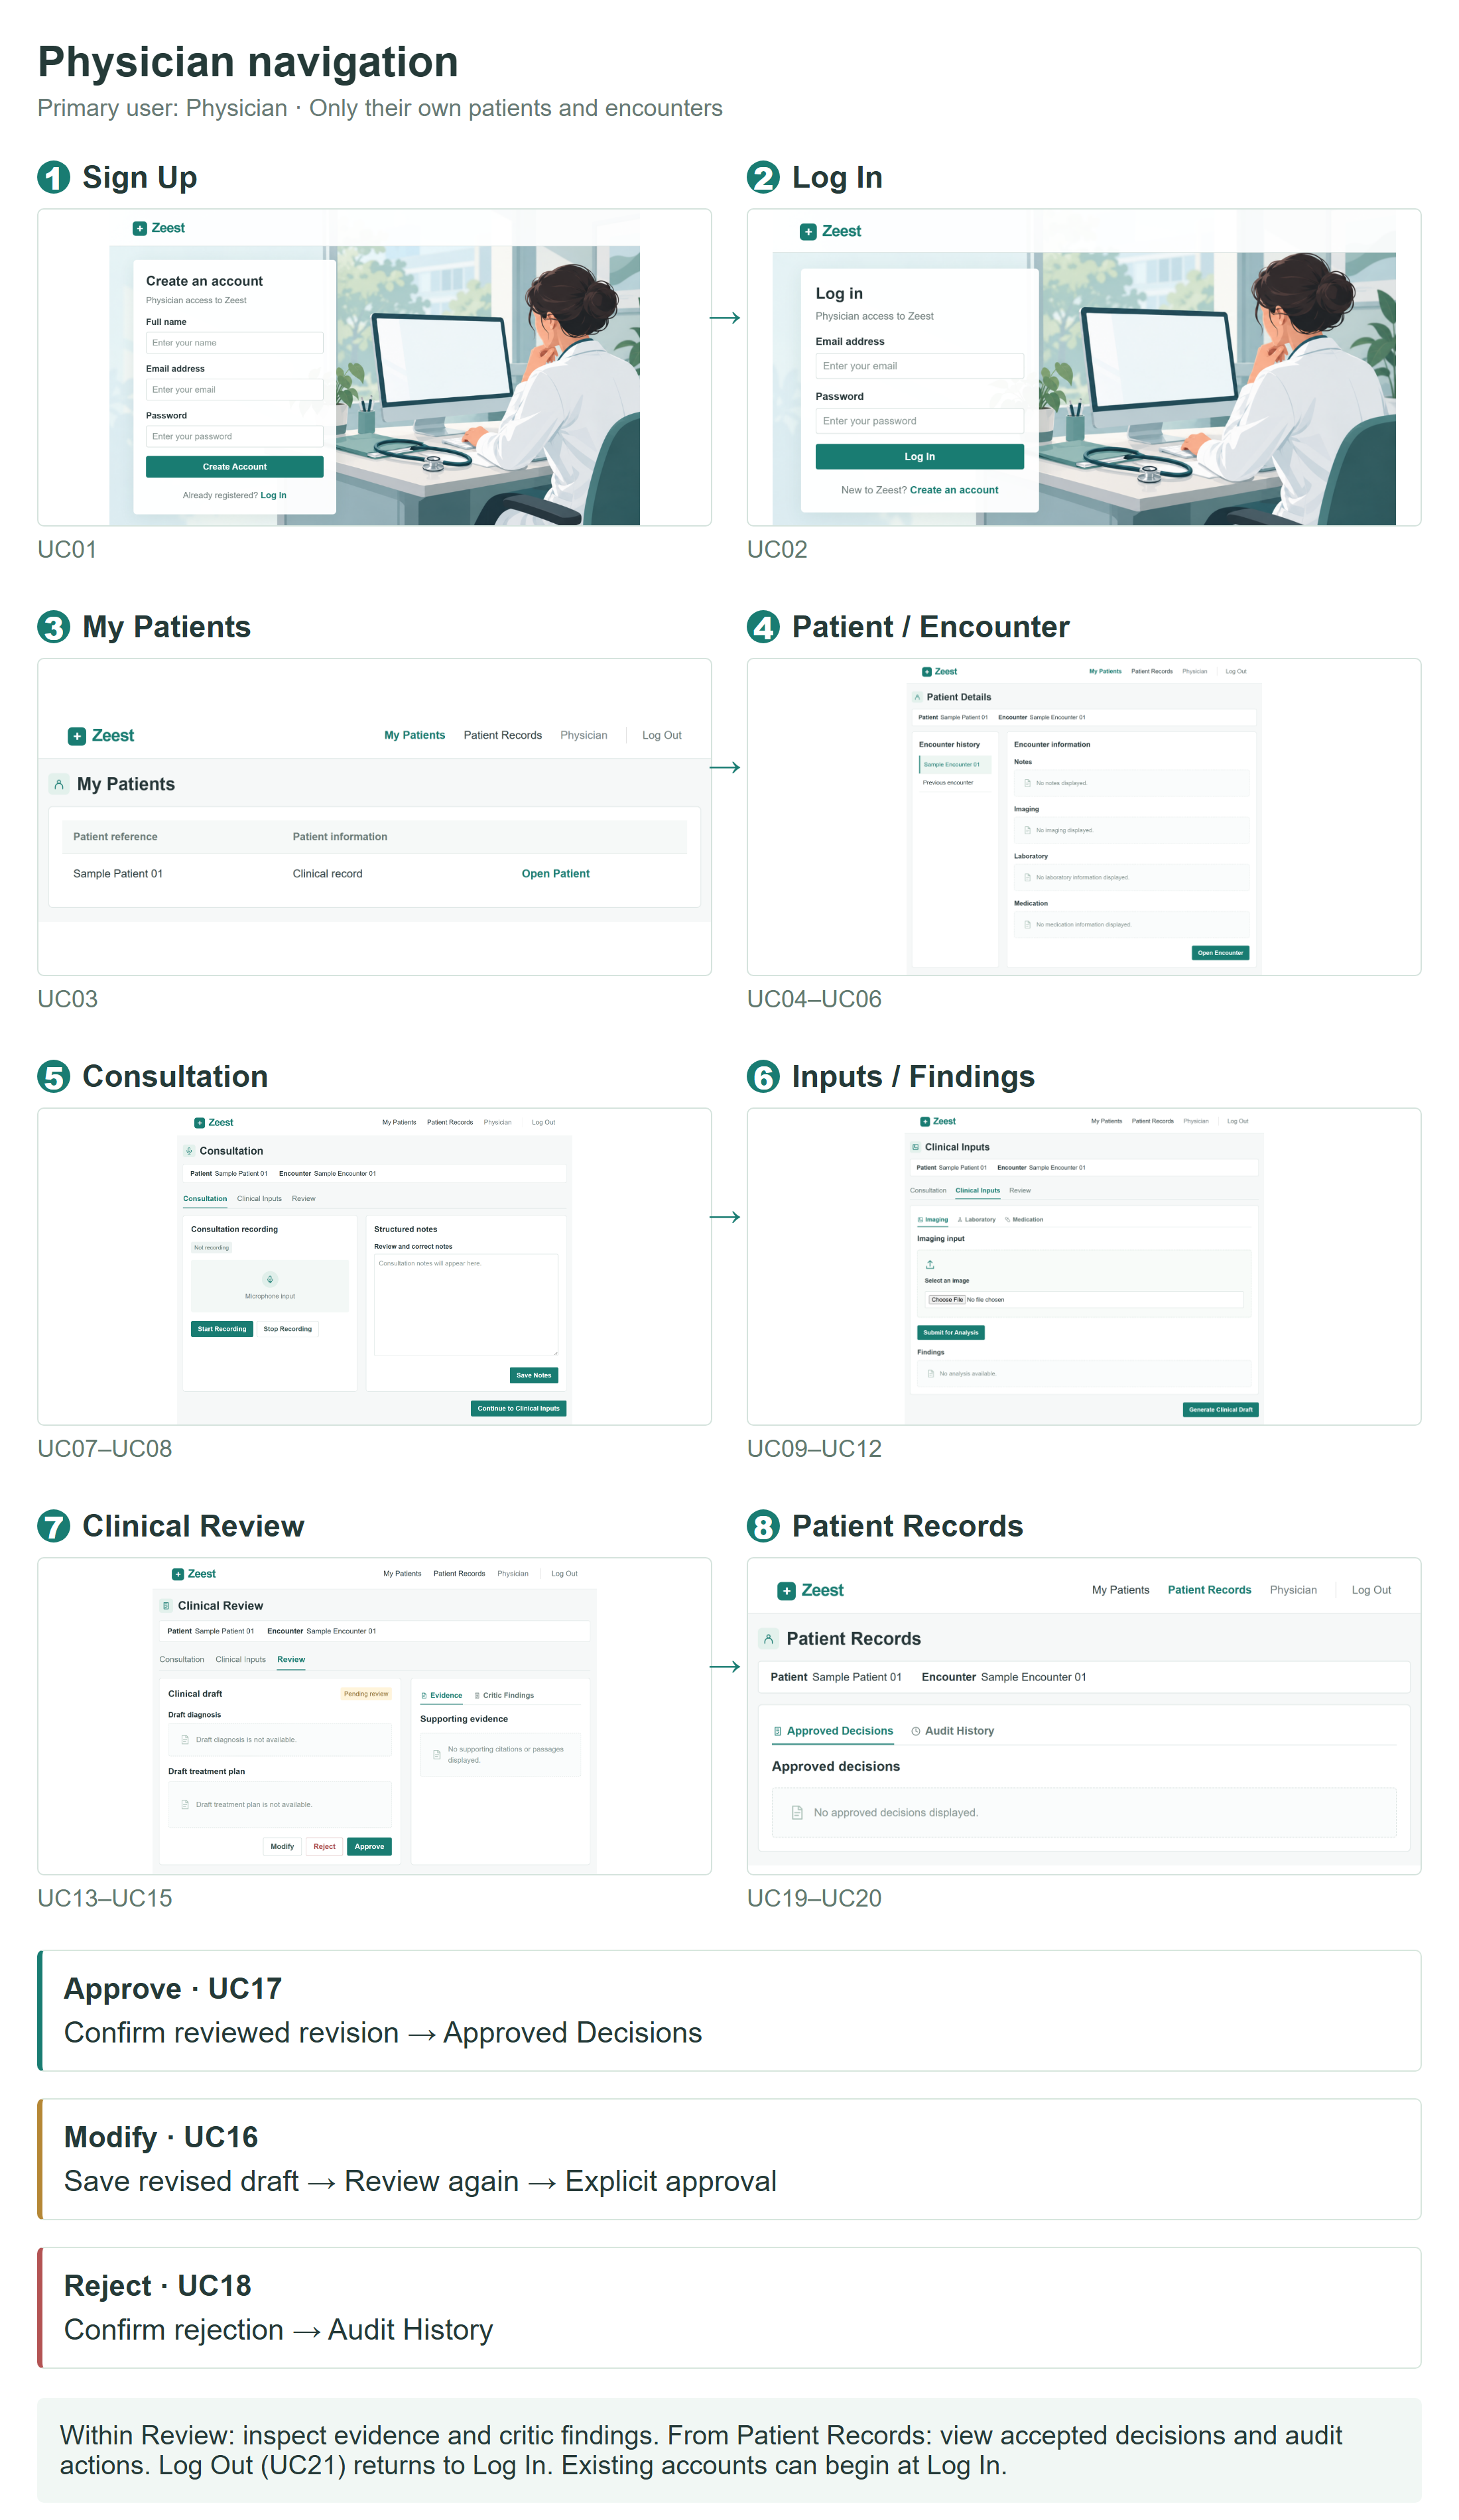
\includegraphics[width=\textwidth,height=0.80\textheight,keepaspectratio]{Figures/kashaf_D02_primary_navigation.png}
\caption{Primary physician navigation through the numbered screen thumbnails. Review branches to modification, approval or rejection; Patient Records exposes approved decisions and audit history. Logout returns to Login.}
\label{fig:kashaf:navigation}
\end{figure}

\begin{figure}[!htbp]
\centering
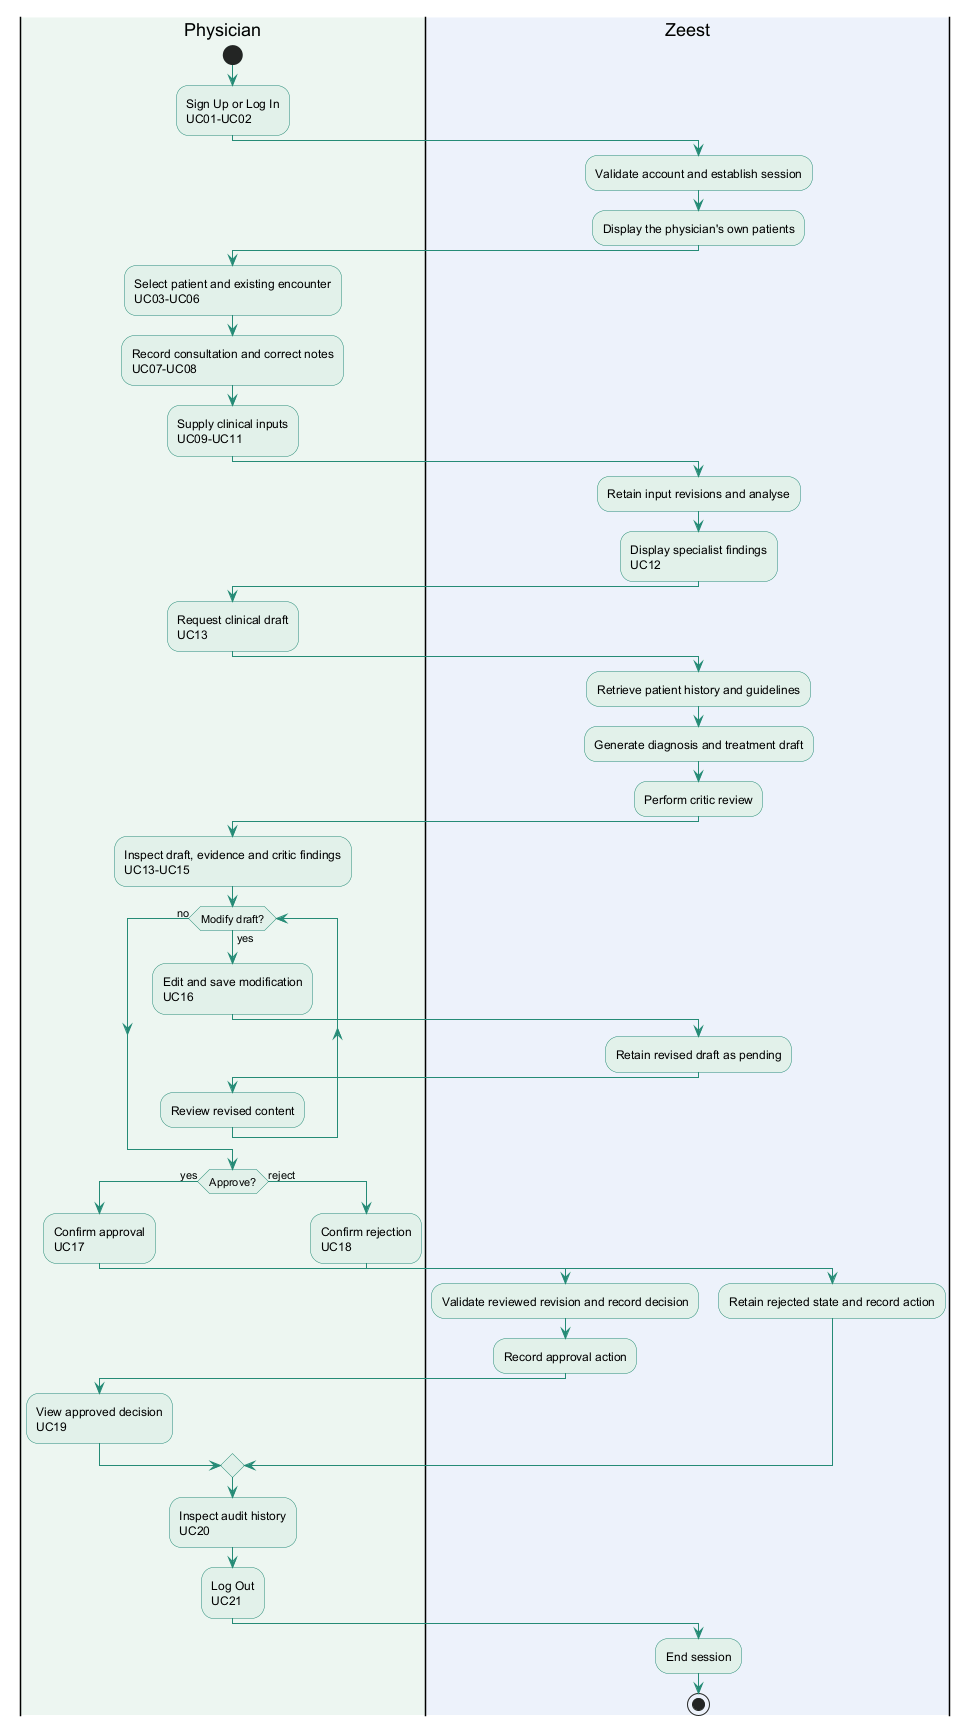
\includegraphics[width=0.96\textwidth,height=0.86\textheight,keepaspectratio]{Figures/kashaf_D02_doctor_navigation.png}
\caption{Physician--Zeest swimlane navigation retained alongside the screen-thumbnail flow. Physician actions appear in the left lane and system processing in the right, including ownership checks, clinical analysis, draft modification, explicit approval or rejection, audit review and logout.}
\label{fig:kashaf:swimlane-navigation}
\end{figure}

\begin{figure}[!htbp]
\centering
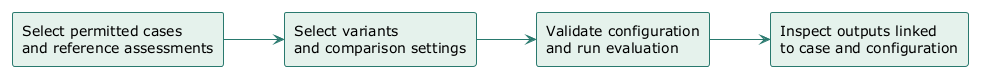
\includegraphics[width=0.96\textwidth,height=.22\textheight,keepaspectratio]{Figures/kashaf_research_navigation.png}
\caption{Research-team navigation for UC22: select permitted cases, configure variants, validate and run evaluation, then inspect outputs associated with each case and configuration.}
\label{fig:kashaf:research-navigation}
\end{figure}

\begin{figure}[!htbp]
\centering
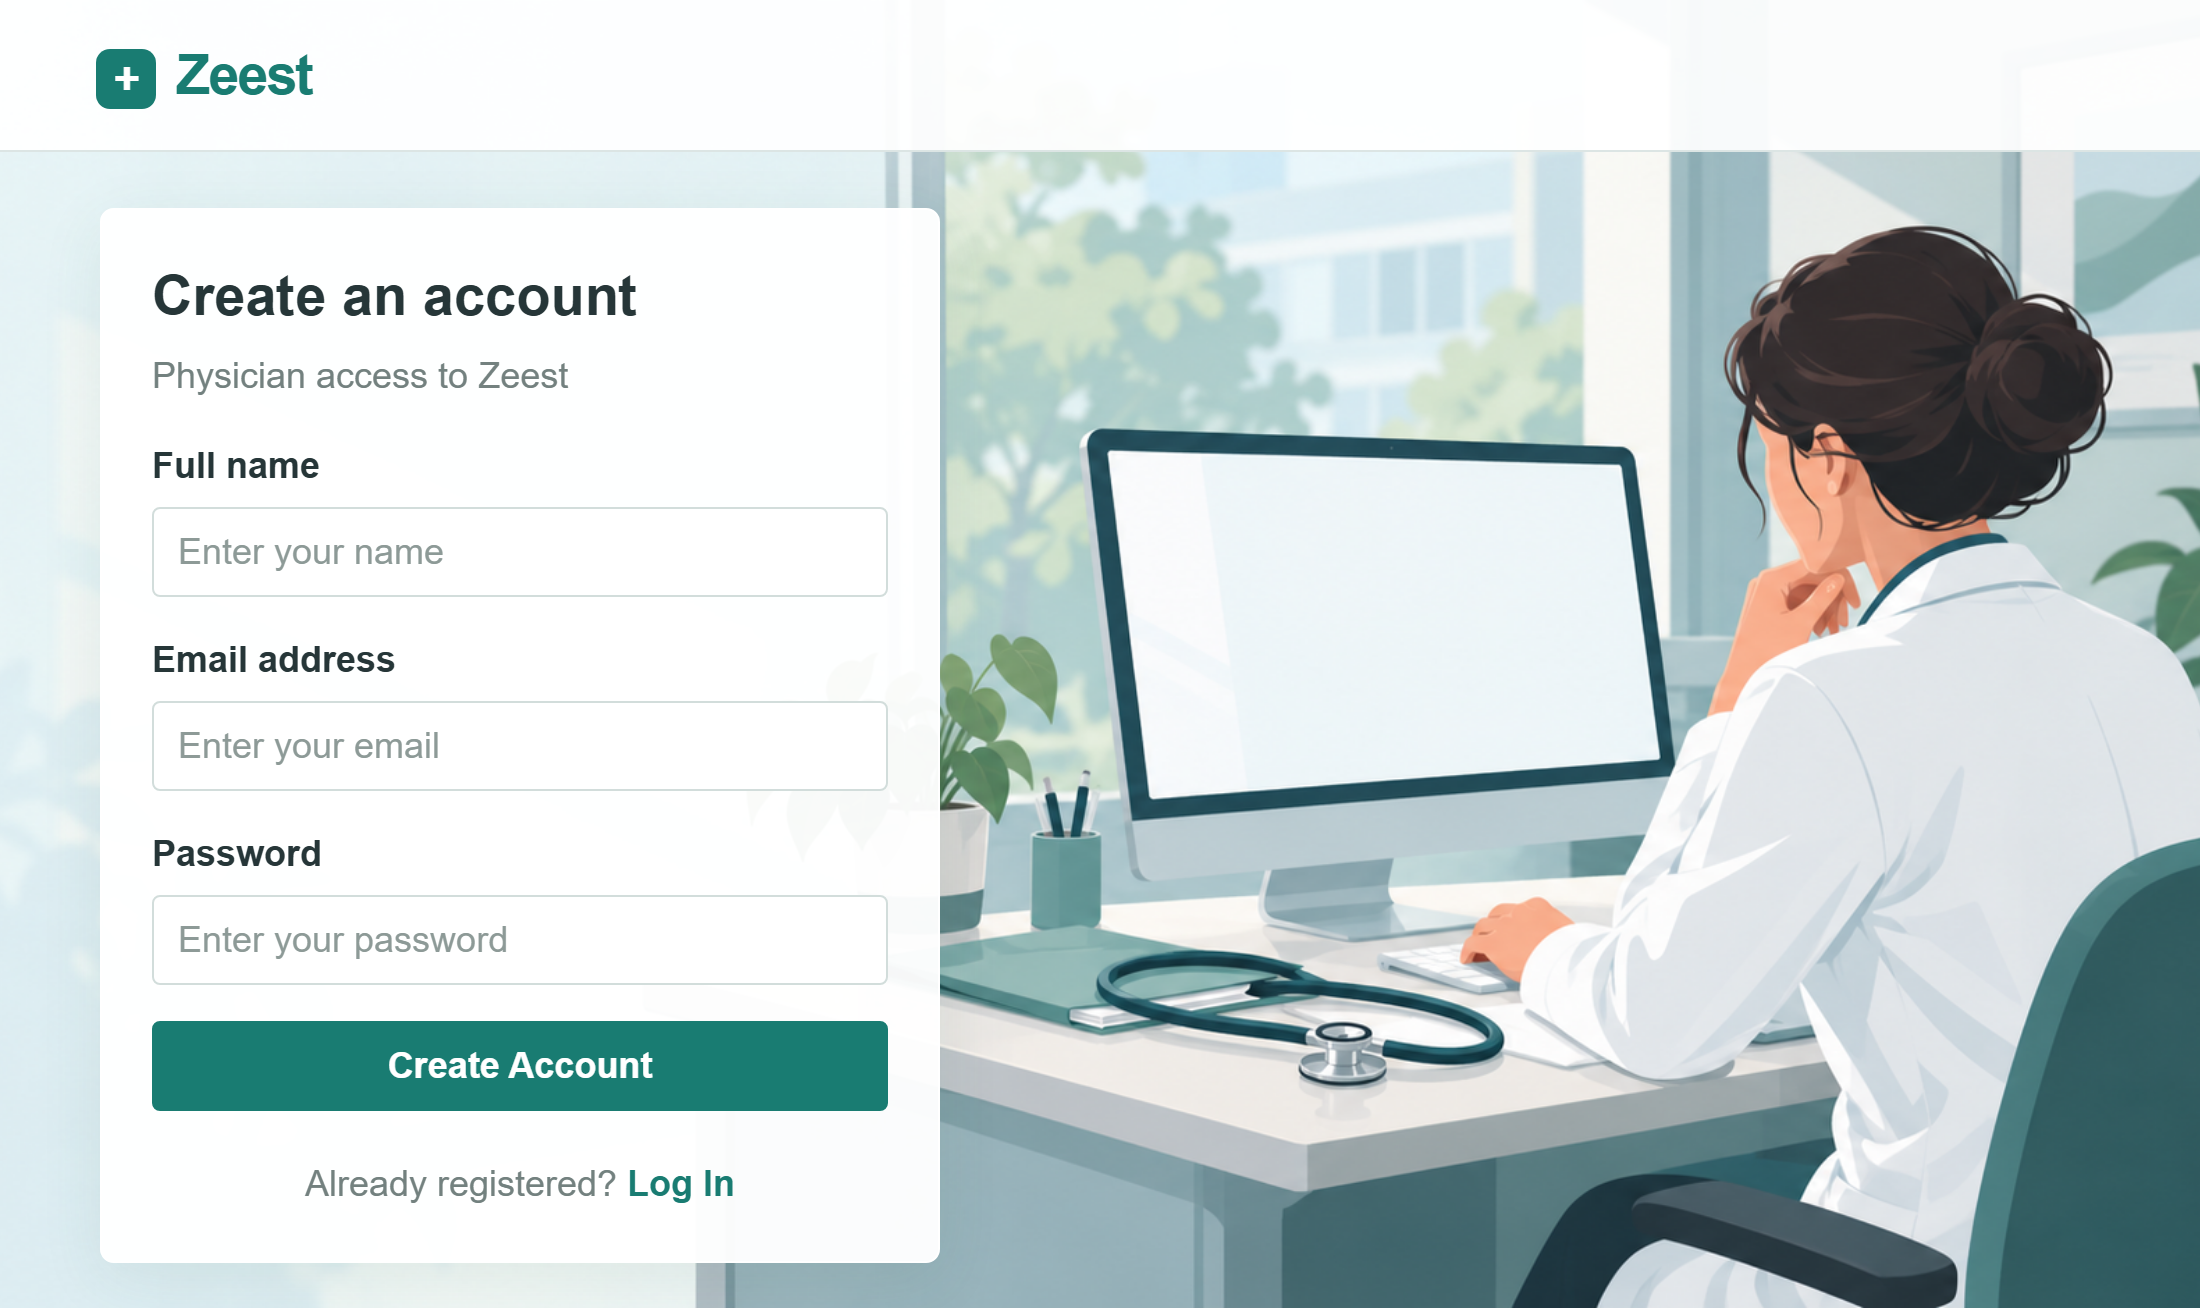
\includegraphics[width=0.96\textwidth,keepaspectratio]{Figures/kashaf_G01_signup.png}
\caption{Physician registration form with name, email and password fields (UC01).}
\label{fig:kashaf:gui-signup}

\centering
\vspace{10pt}
\centering
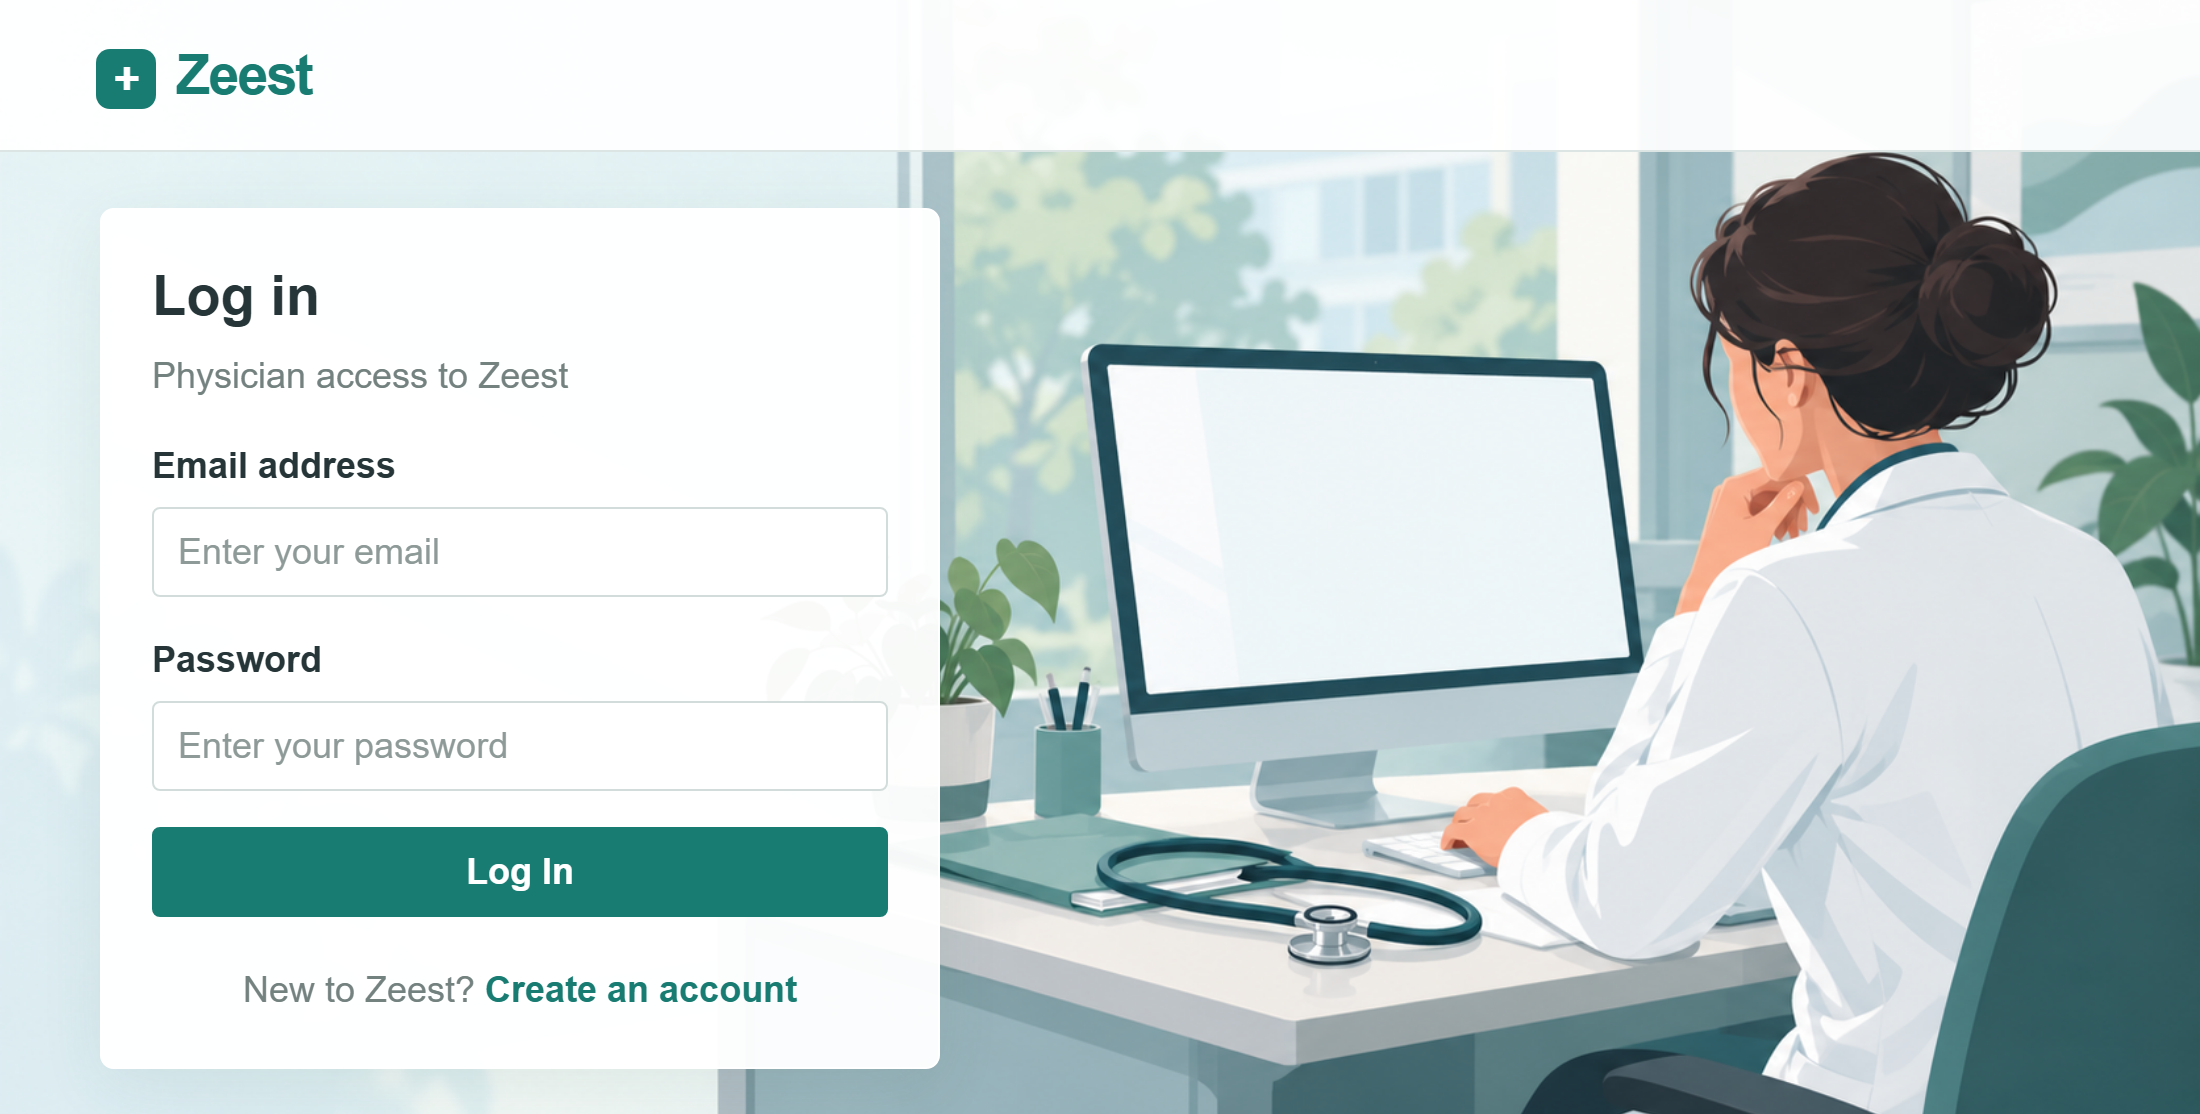
\includegraphics[width=0.96\textwidth,keepaspectratio]{Figures/kashaf_G02_login.png}
\caption{Physician login form and account-access controls (UC02, UC21).}
\label{fig:kashaf:gui-login}
\end{figure}

\begin{figure}[!htbp]
\centering
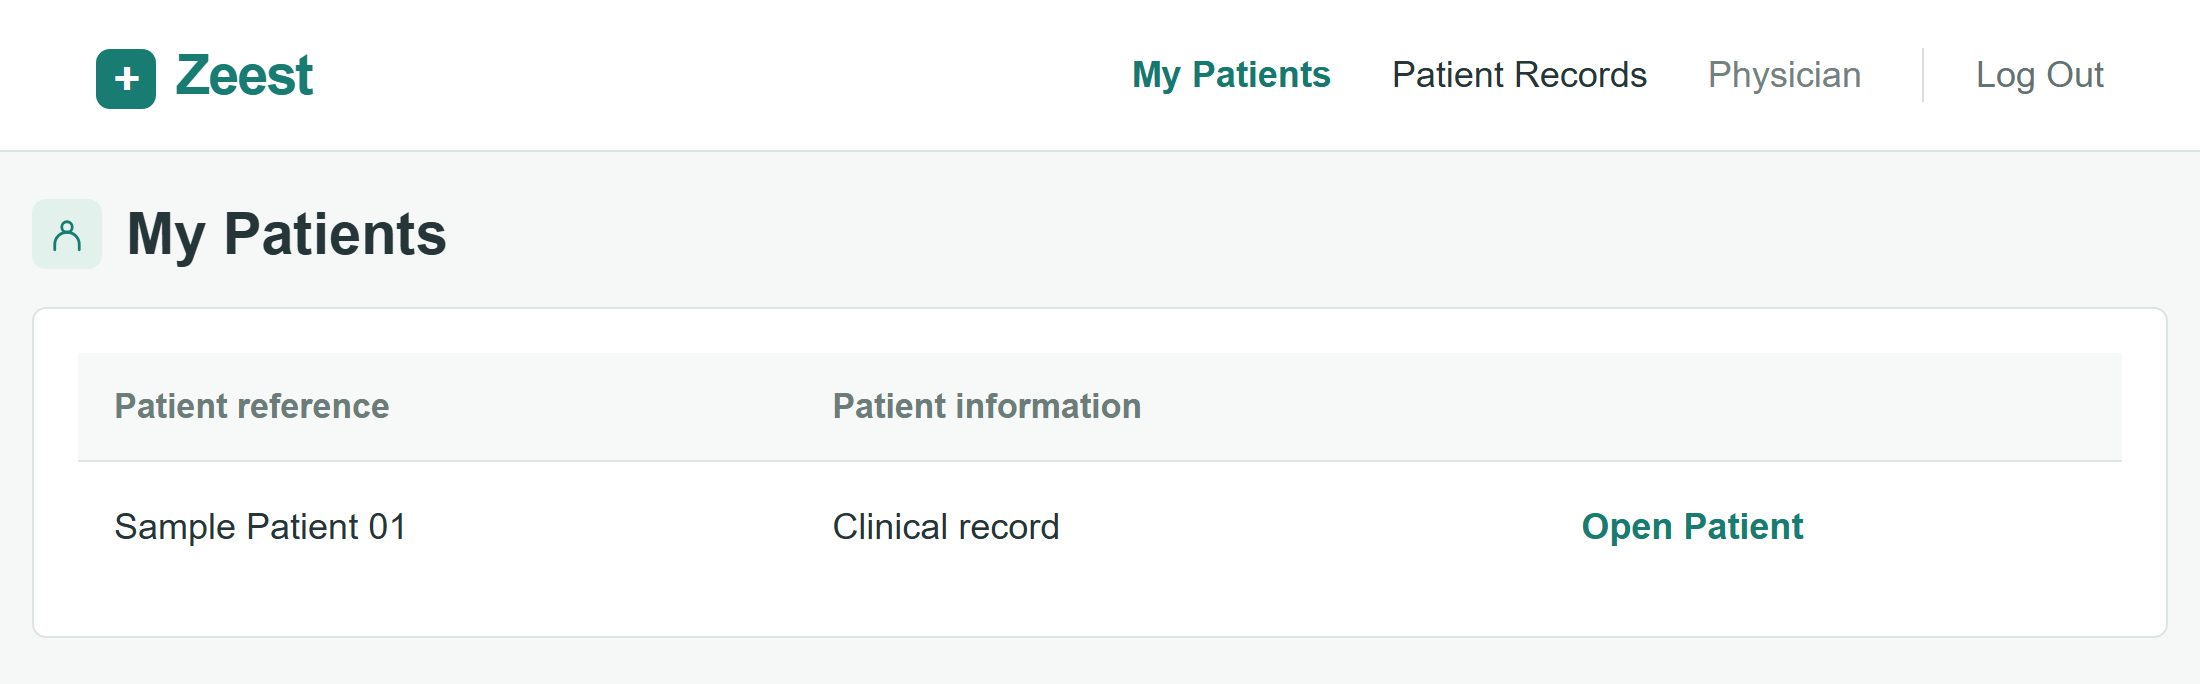
\includegraphics[width=0.96\textwidth,keepaspectratio]{Figures/kashaf_G03_patients.png}
\caption{Physician patient list and selection controls (UC03, UC21).}
\label{fig:kashaf:gui-patients}

\centering
\vspace{10pt}
\centering
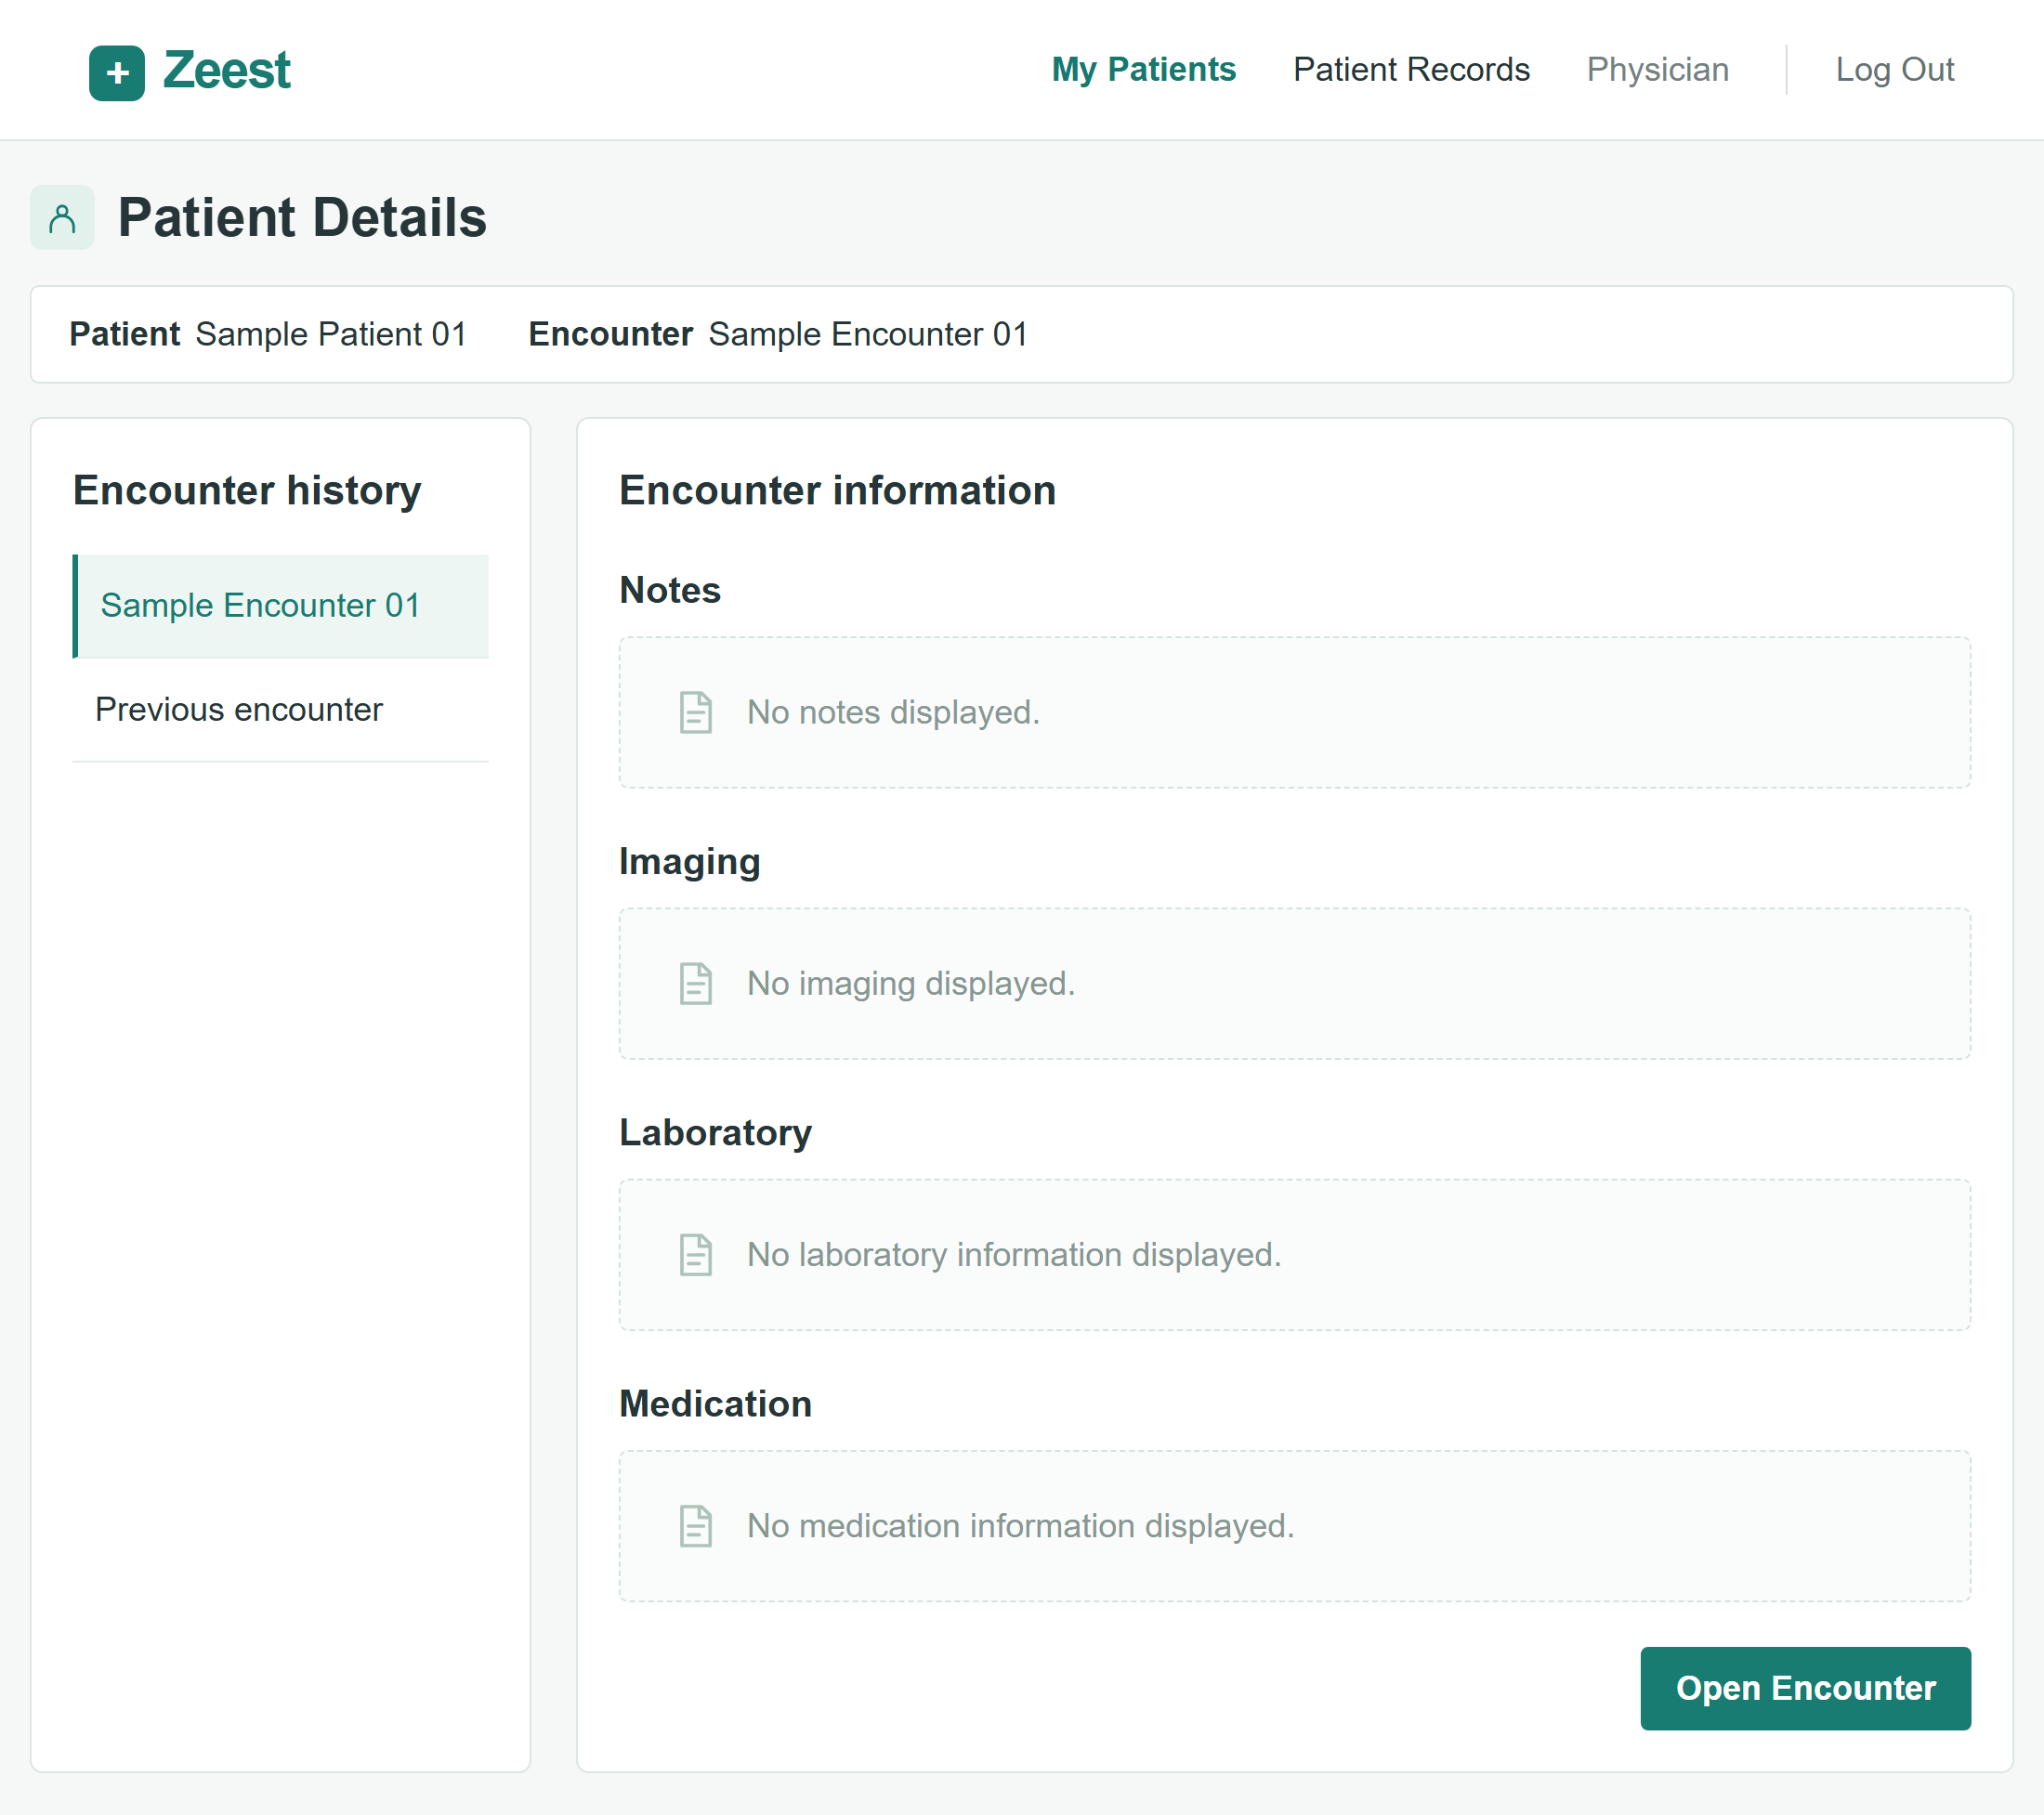
\includegraphics[width=0.96\textwidth,keepaspectratio]{Figures/kashaf_G04_history.png}
\caption{Patient context, history and encounter selection (Physician, UC04--UC06).}
\label{fig:kashaf:gui-history}
\end{figure}

\begin{figure}[!htbp]
\centering
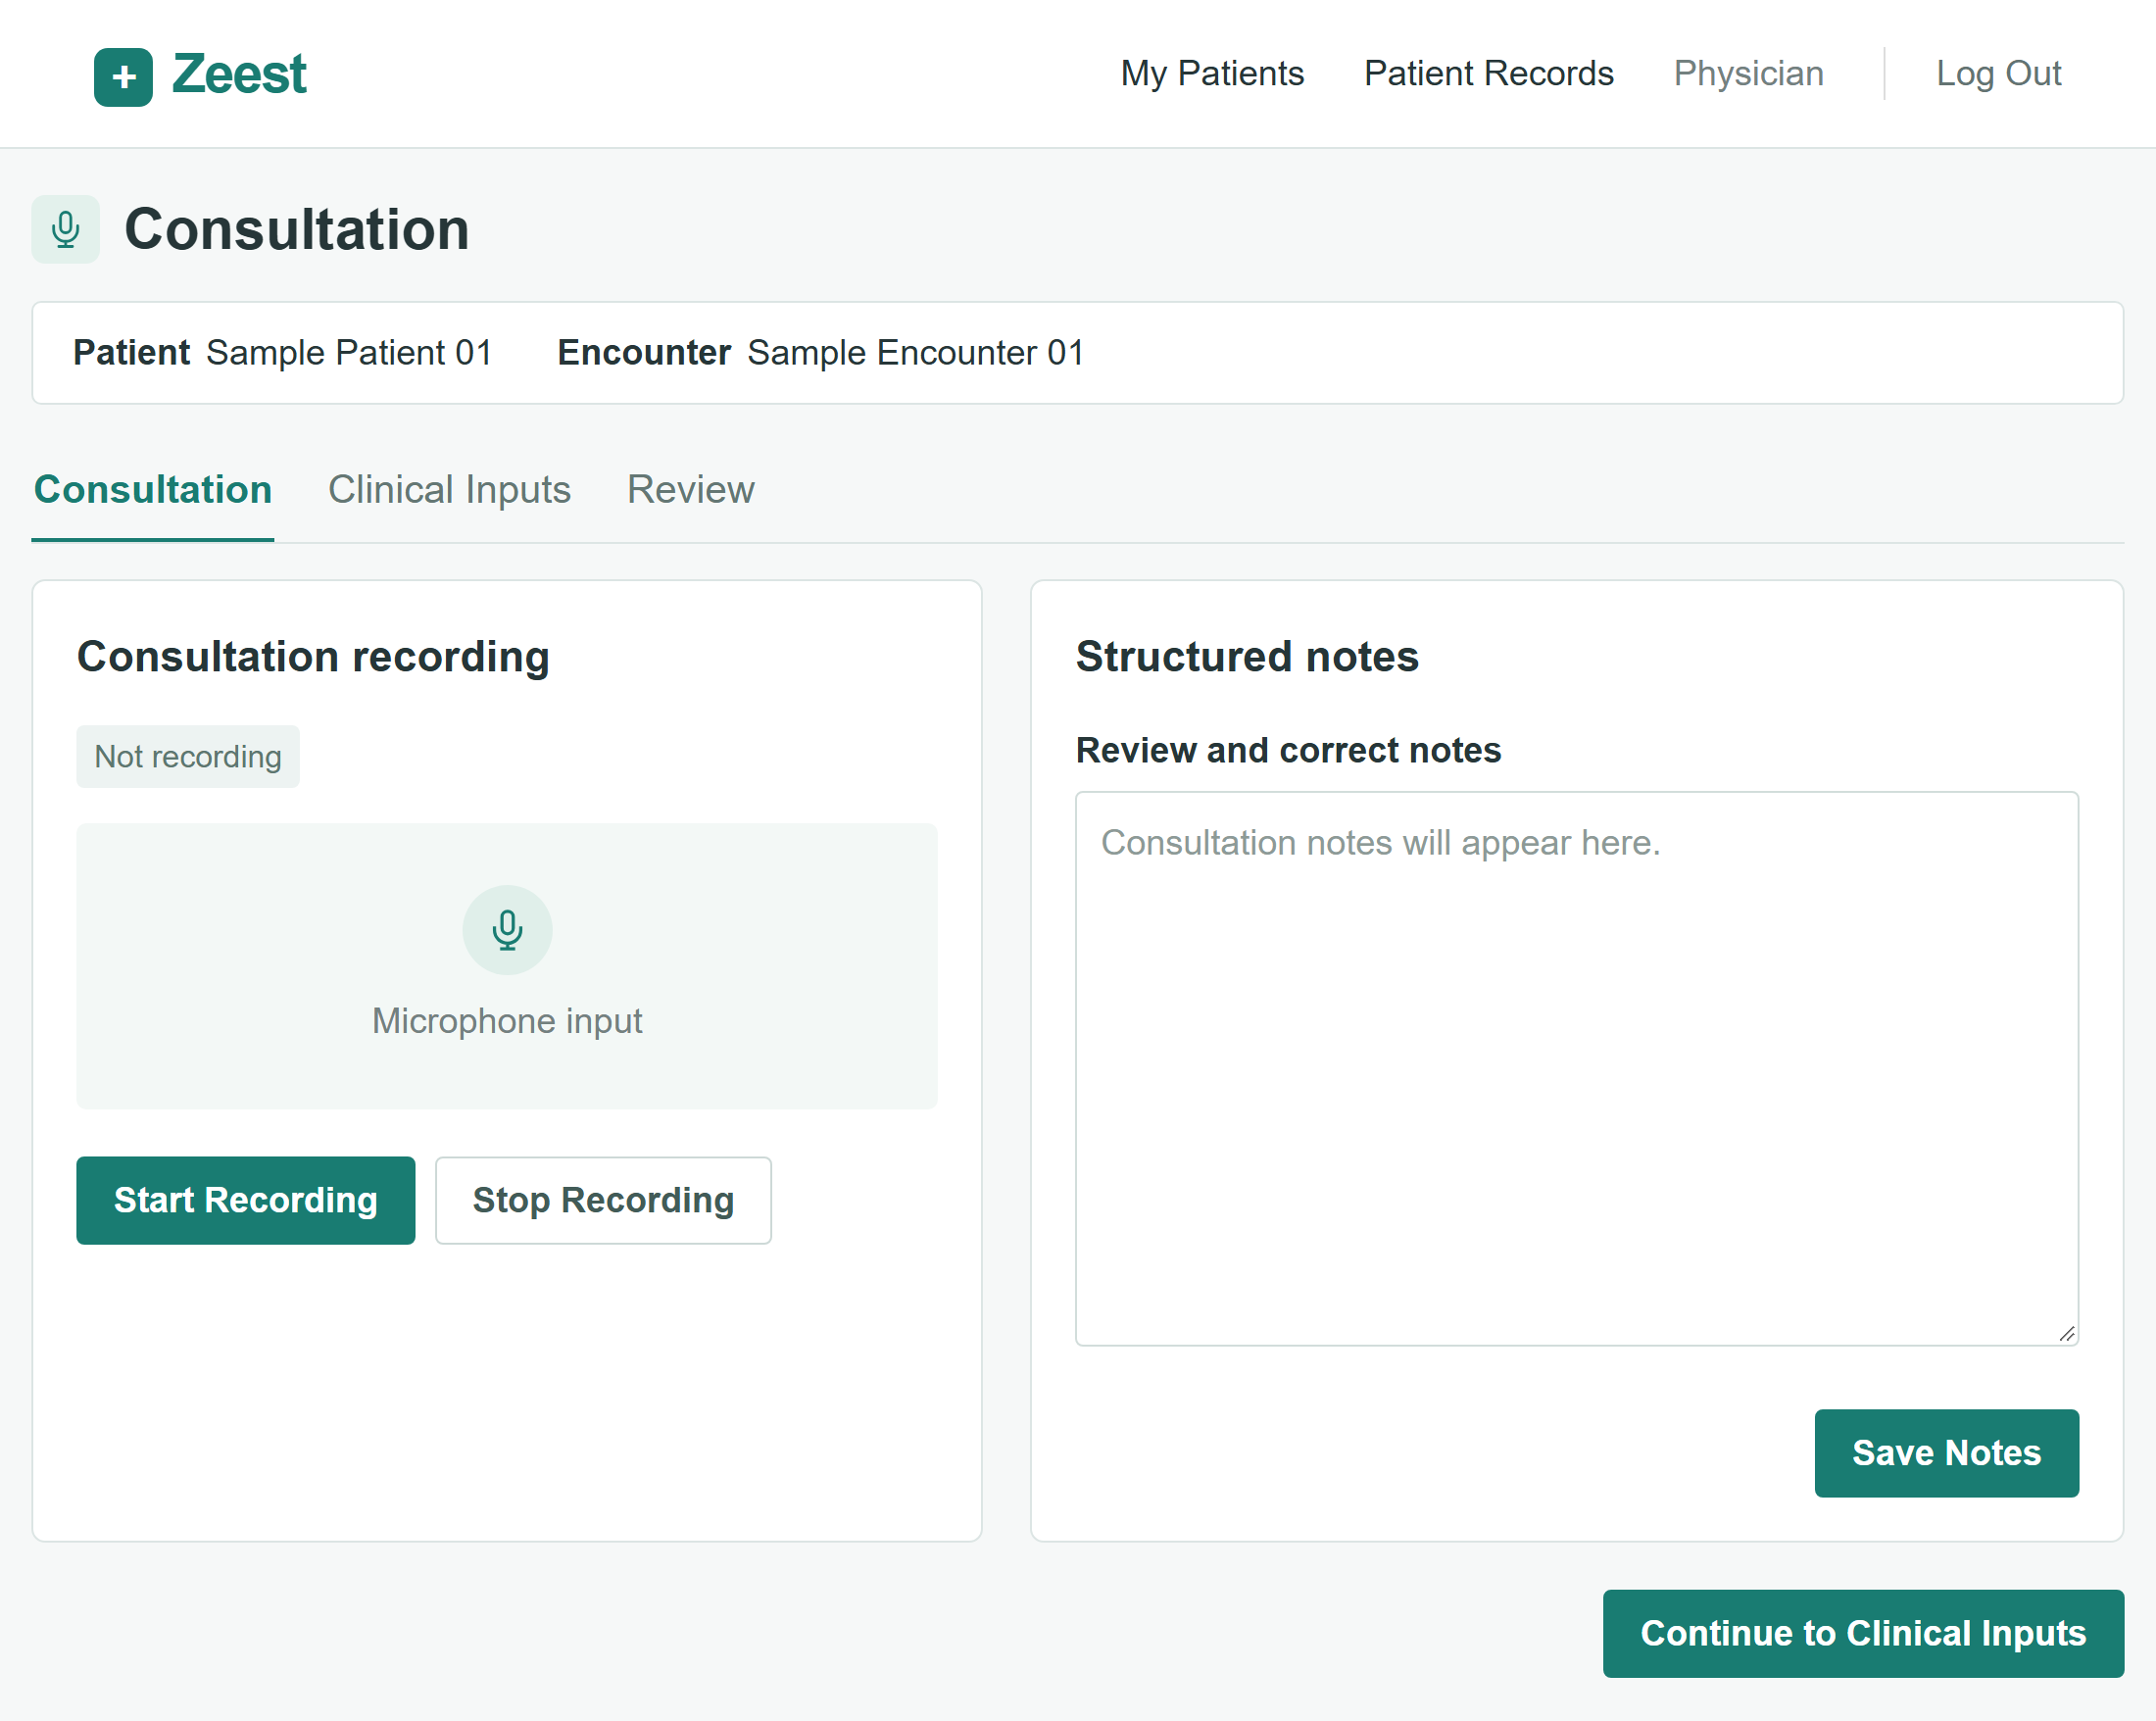
\includegraphics[width=0.96\textwidth,height=.88\textheight,keepaspectratio]{Figures/kashaf_G05_consultation.png}
\caption{Consultation recording controls and editable notes (Physician, UC07--UC08).}
\label{fig:kashaf:gui-consultation}

\centering
\end{figure}

\begin{figure}[!htbp]
\centering
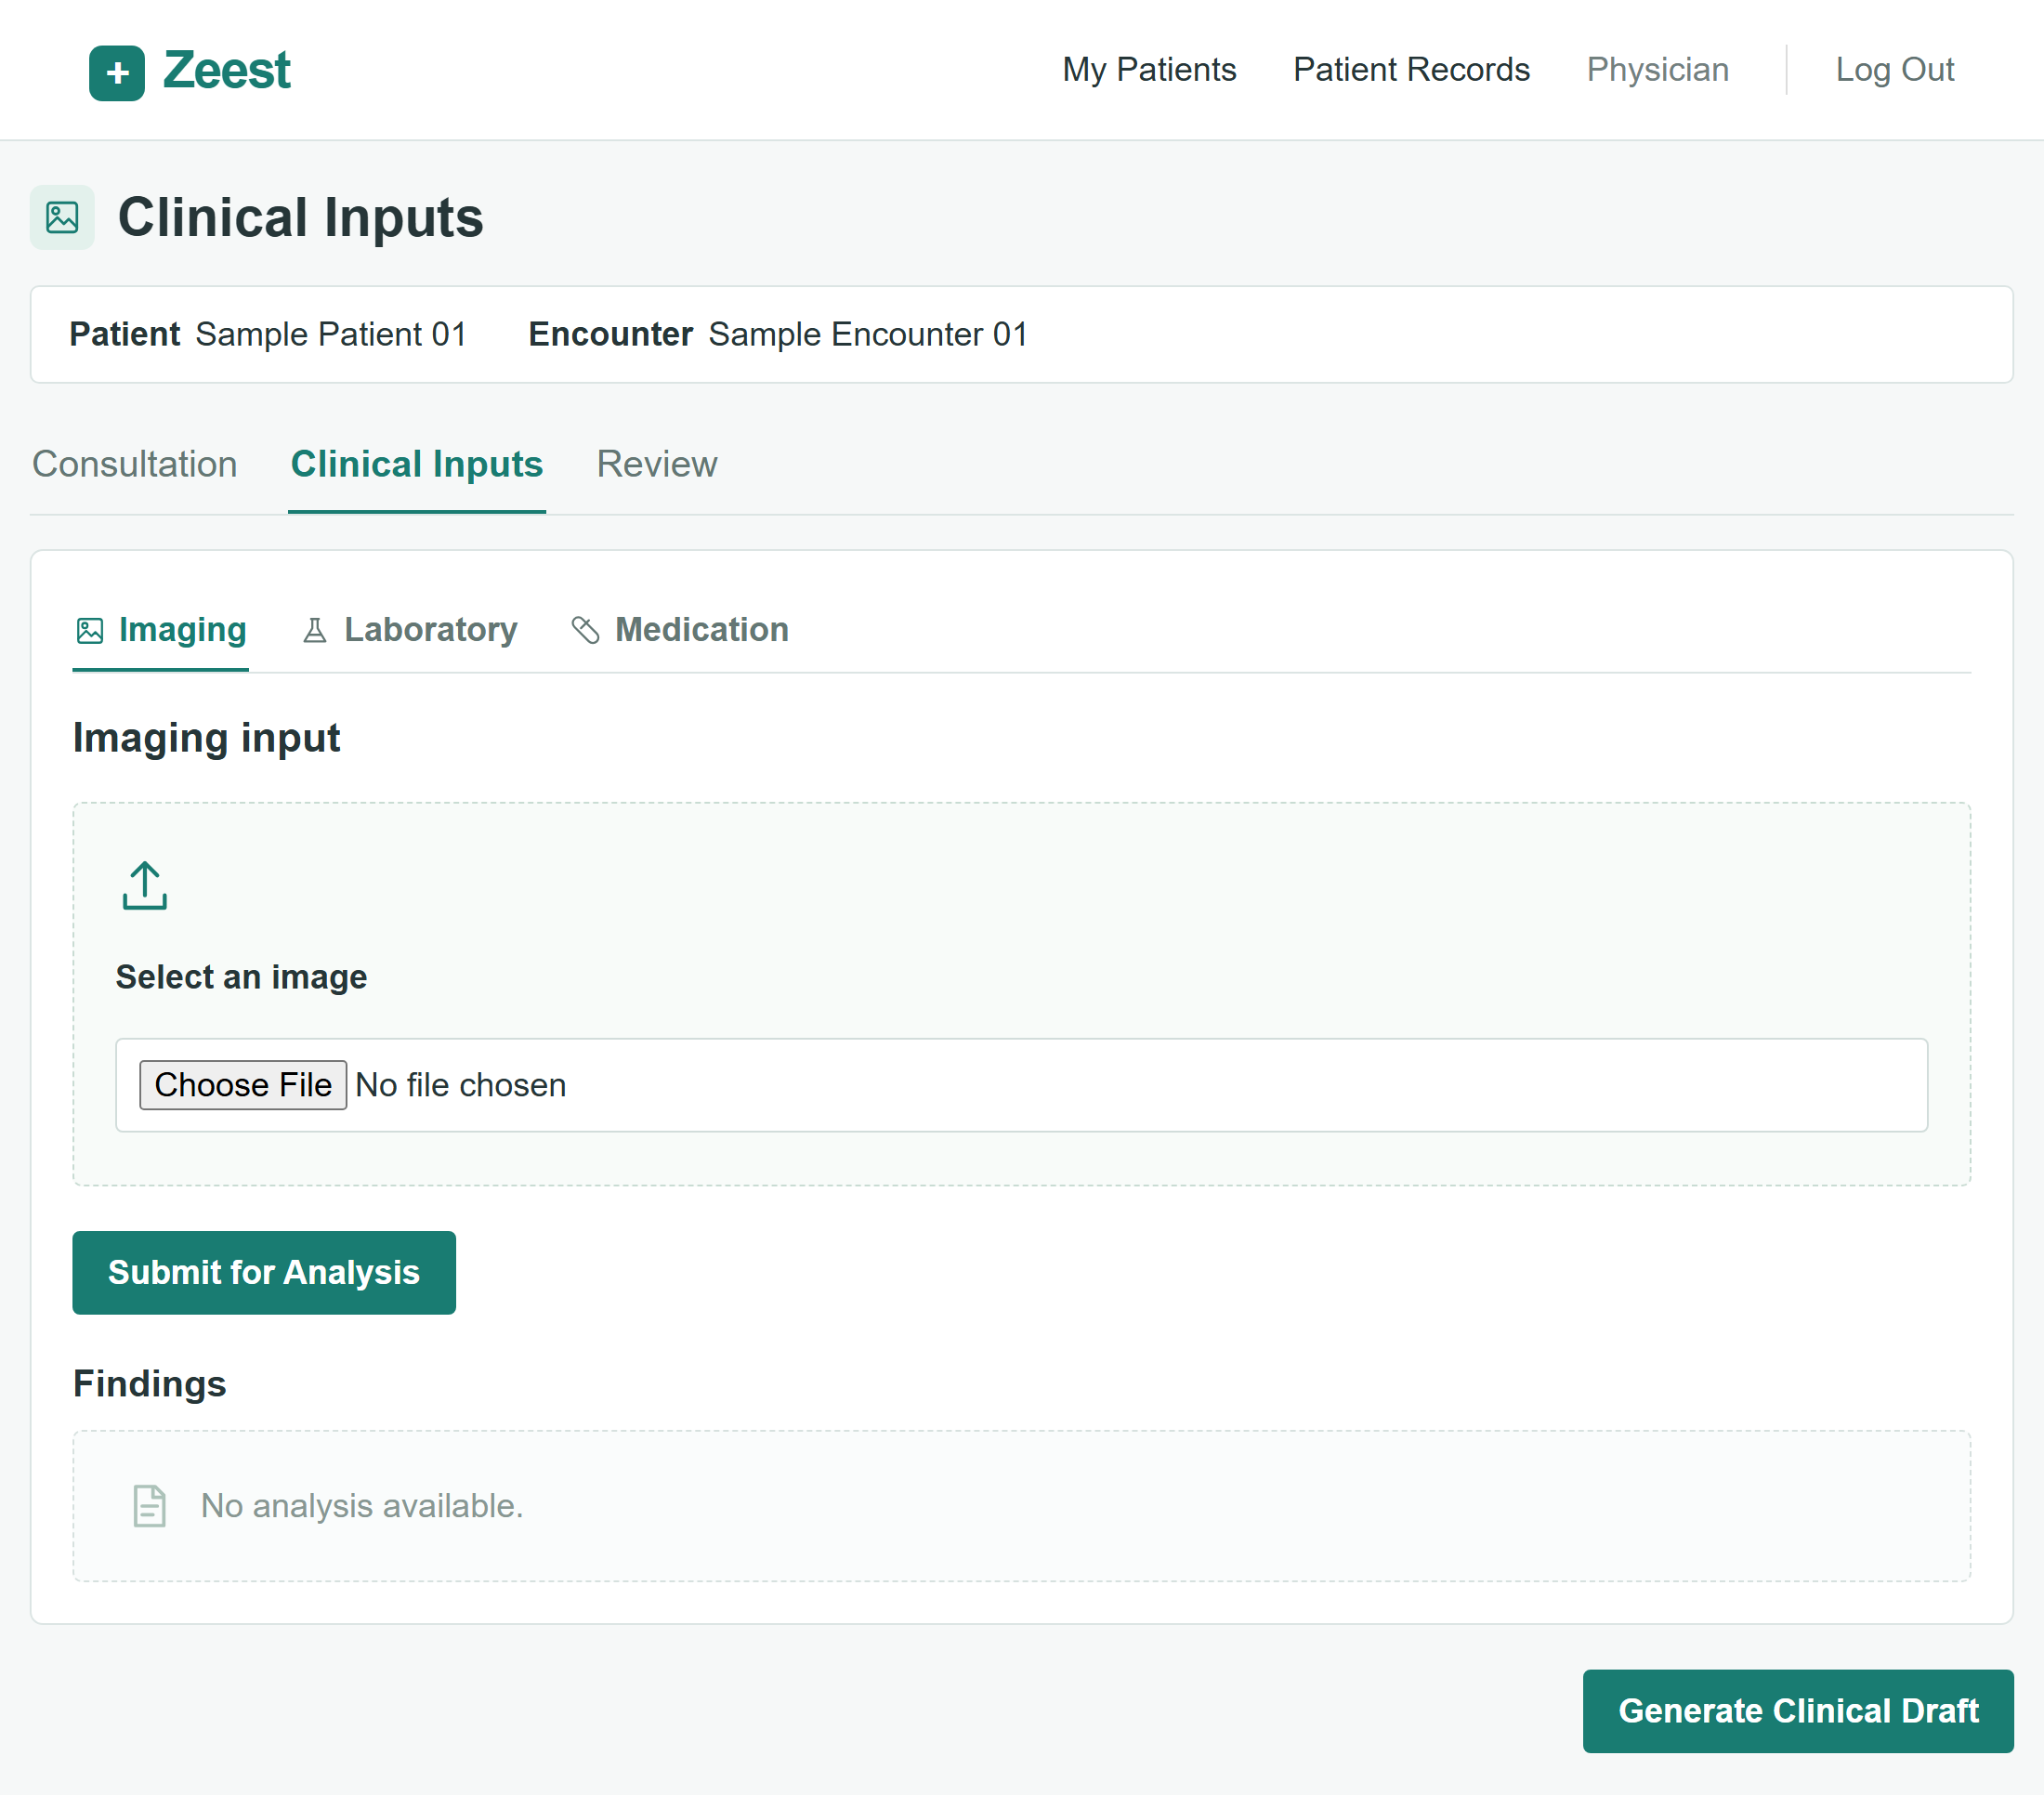
\includegraphics[width=0.96\textwidth,height=.88\textheight,keepaspectratio]{Figures/kashaf_G06_imaging.png}
\caption{Imaging upload and findings area (Physician, UC09, UC12).}
\label{fig:kashaf:gui-imaging}
\end{figure}

\begin{figure}[!htbp]
\centering
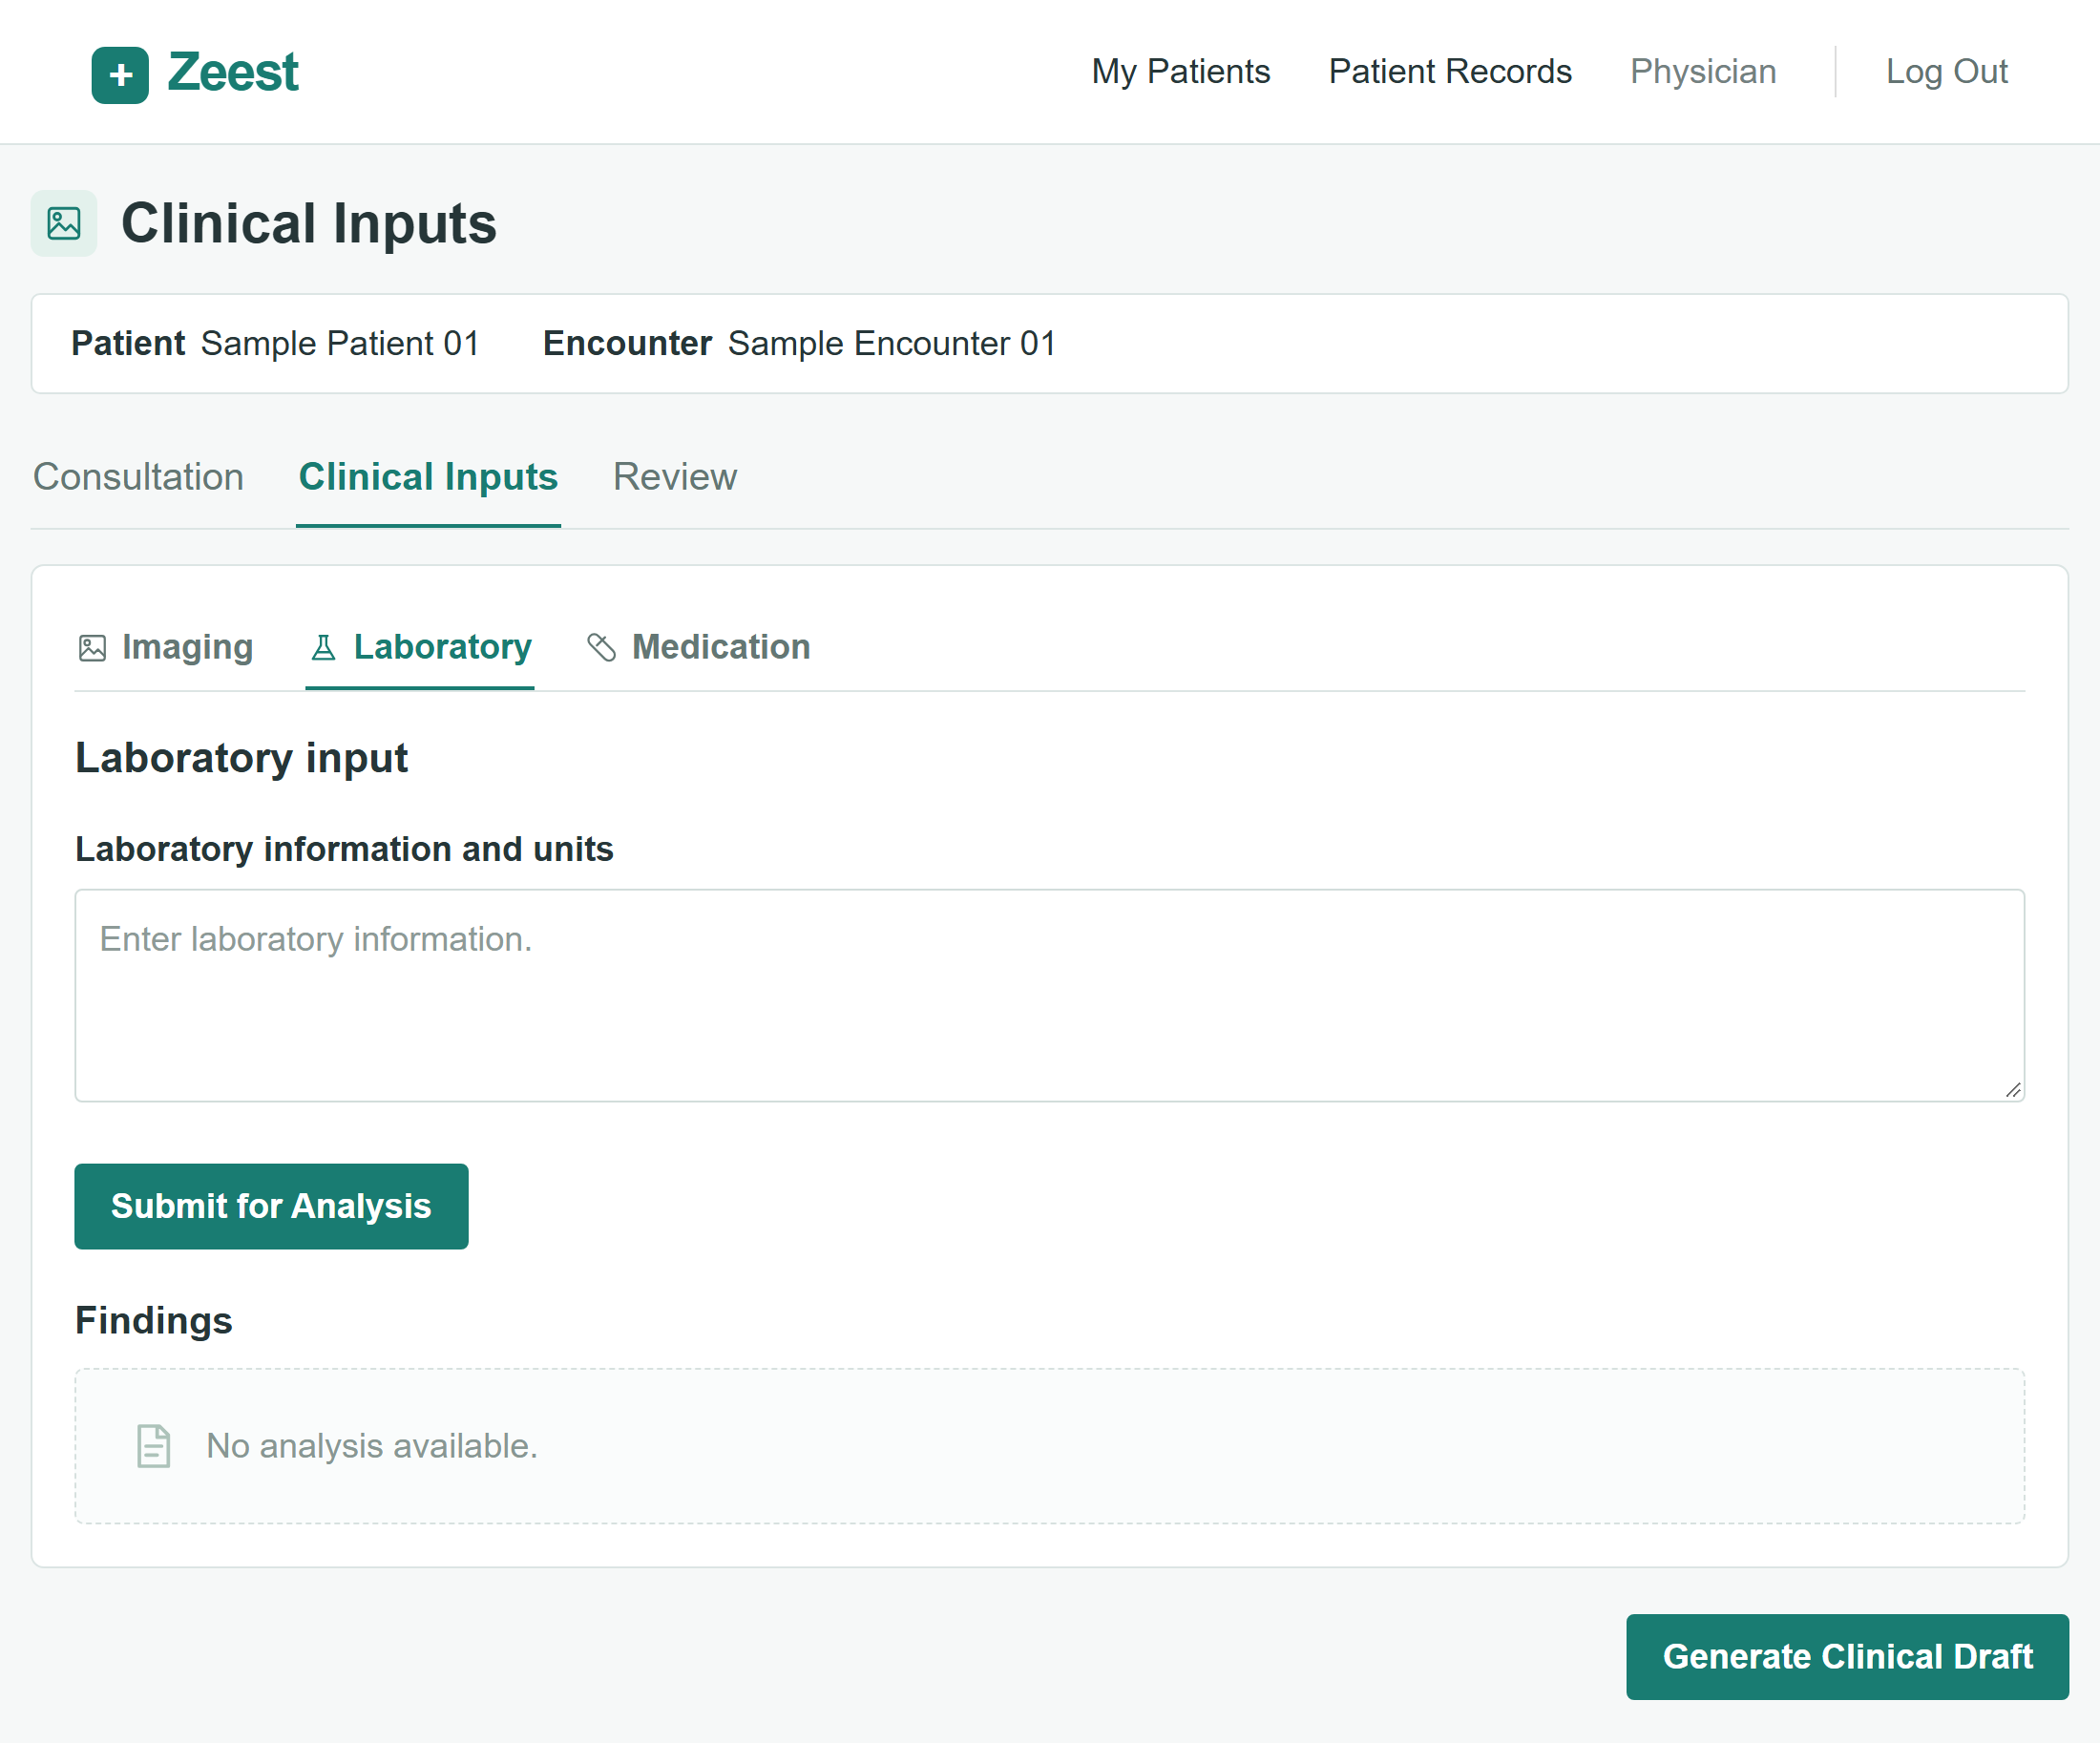
\includegraphics[width=0.96\textwidth,height=.88\textheight,keepaspectratio]{Figures/kashaf_G07_laboratory.png}
\caption{Laboratory input and findings area (Physician, UC10, UC12).}
\label{fig:kashaf:gui-laboratory}

\centering
\end{figure}

\begin{figure}[!htbp]
\centering
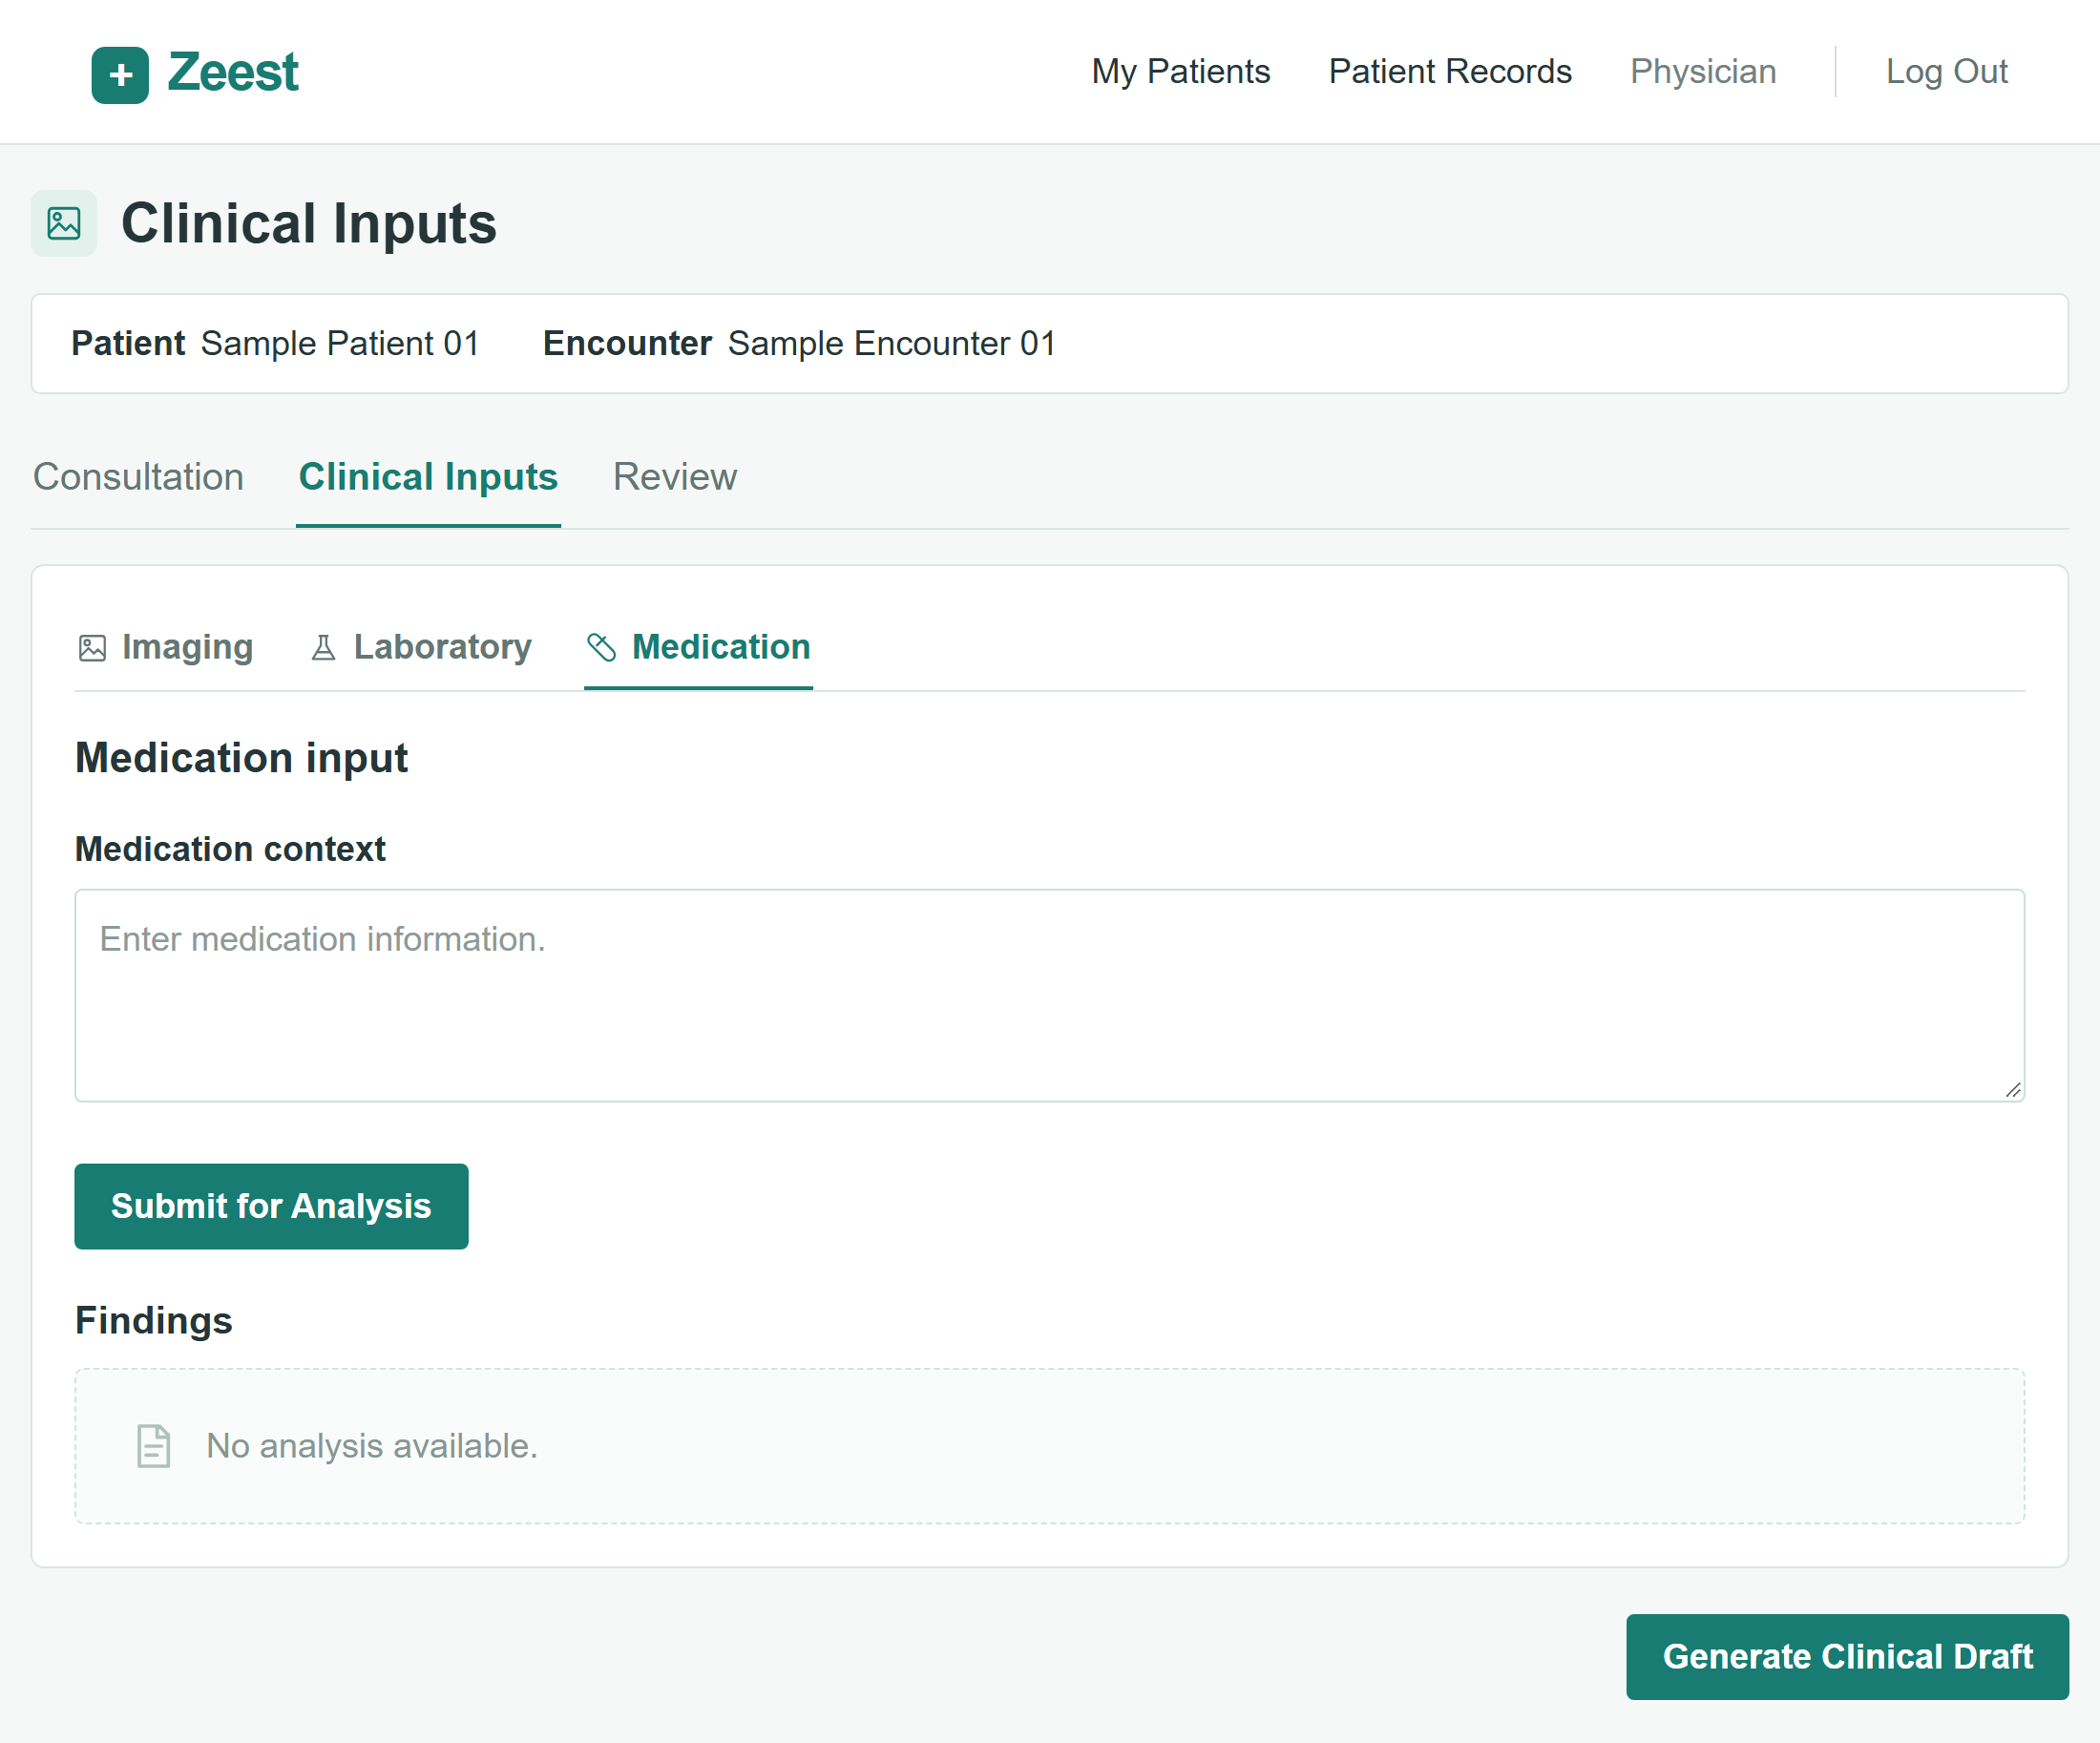
\includegraphics[width=0.96\textwidth,height=.88\textheight,keepaspectratio]{Figures/kashaf_G08_medication.png}
\caption{Medication input and findings area (Physician, UC11, UC12).}
\label{fig:kashaf:gui-medication}
\end{figure}

\begin{figure}[!htbp]
\centering
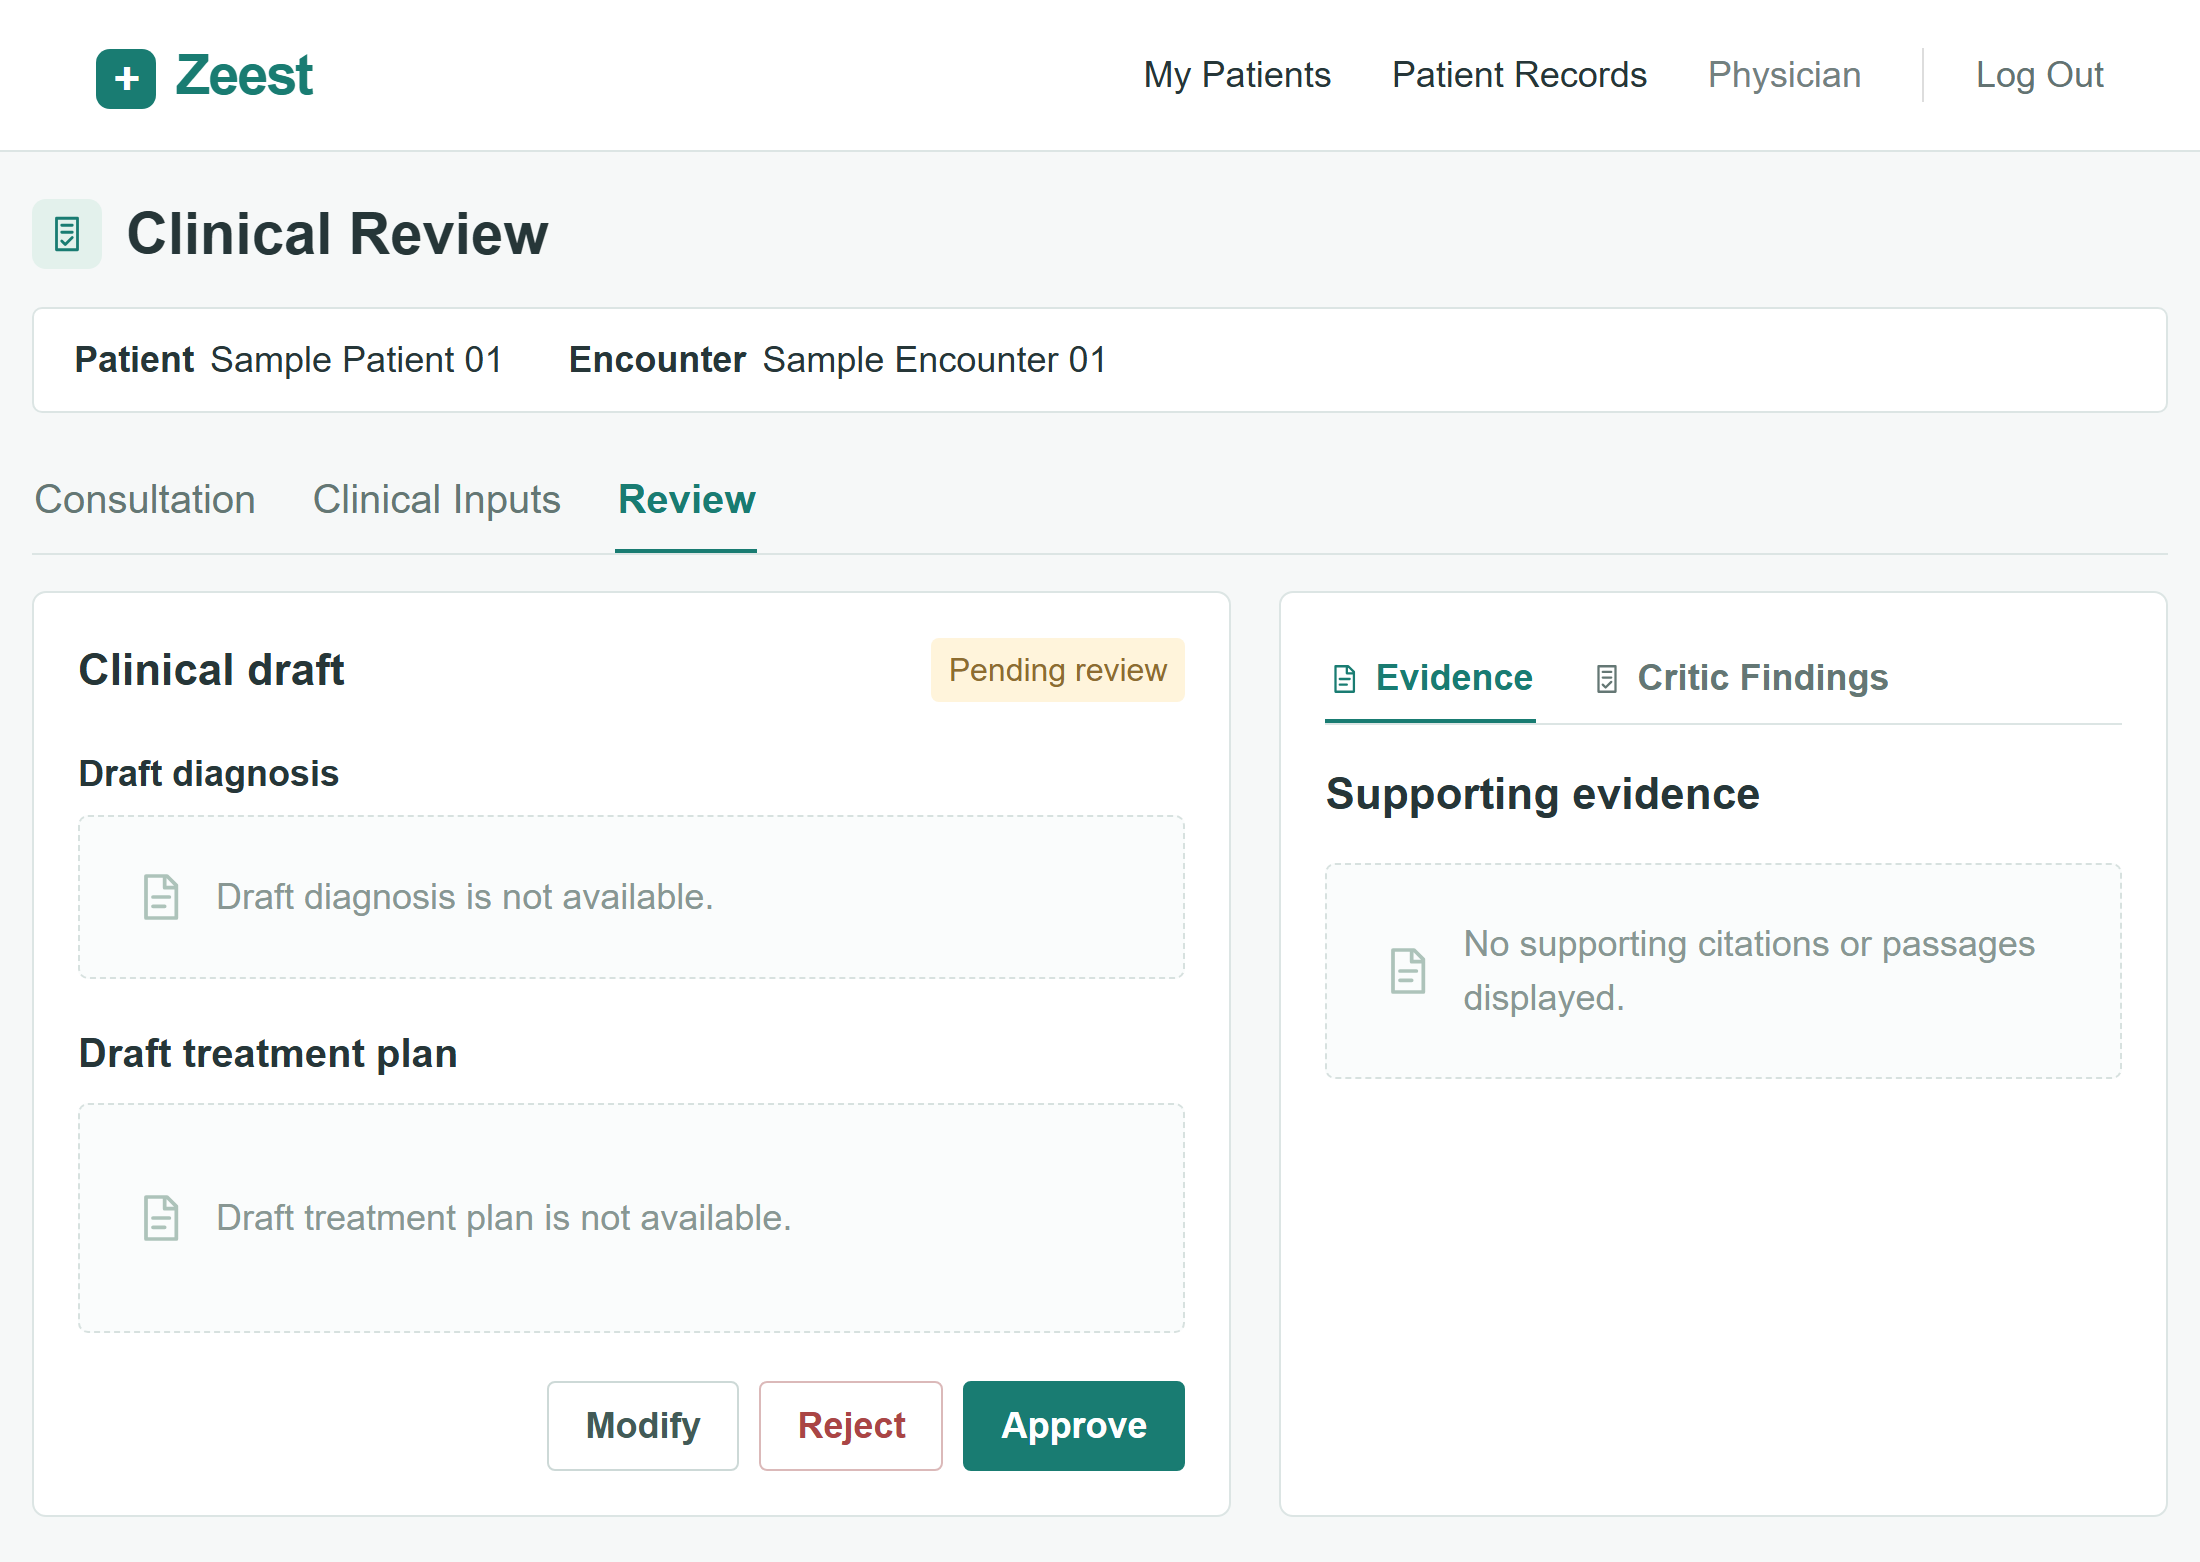
\includegraphics[width=0.96\textwidth,keepaspectratio]{Figures/kashaf_G09_review.png}
\caption{Clinical draft and supporting evidence tabs (Physician, UC13--UC14).}
\label{fig:kashaf:gui-review}

\centering
\vspace{10pt}
\centering
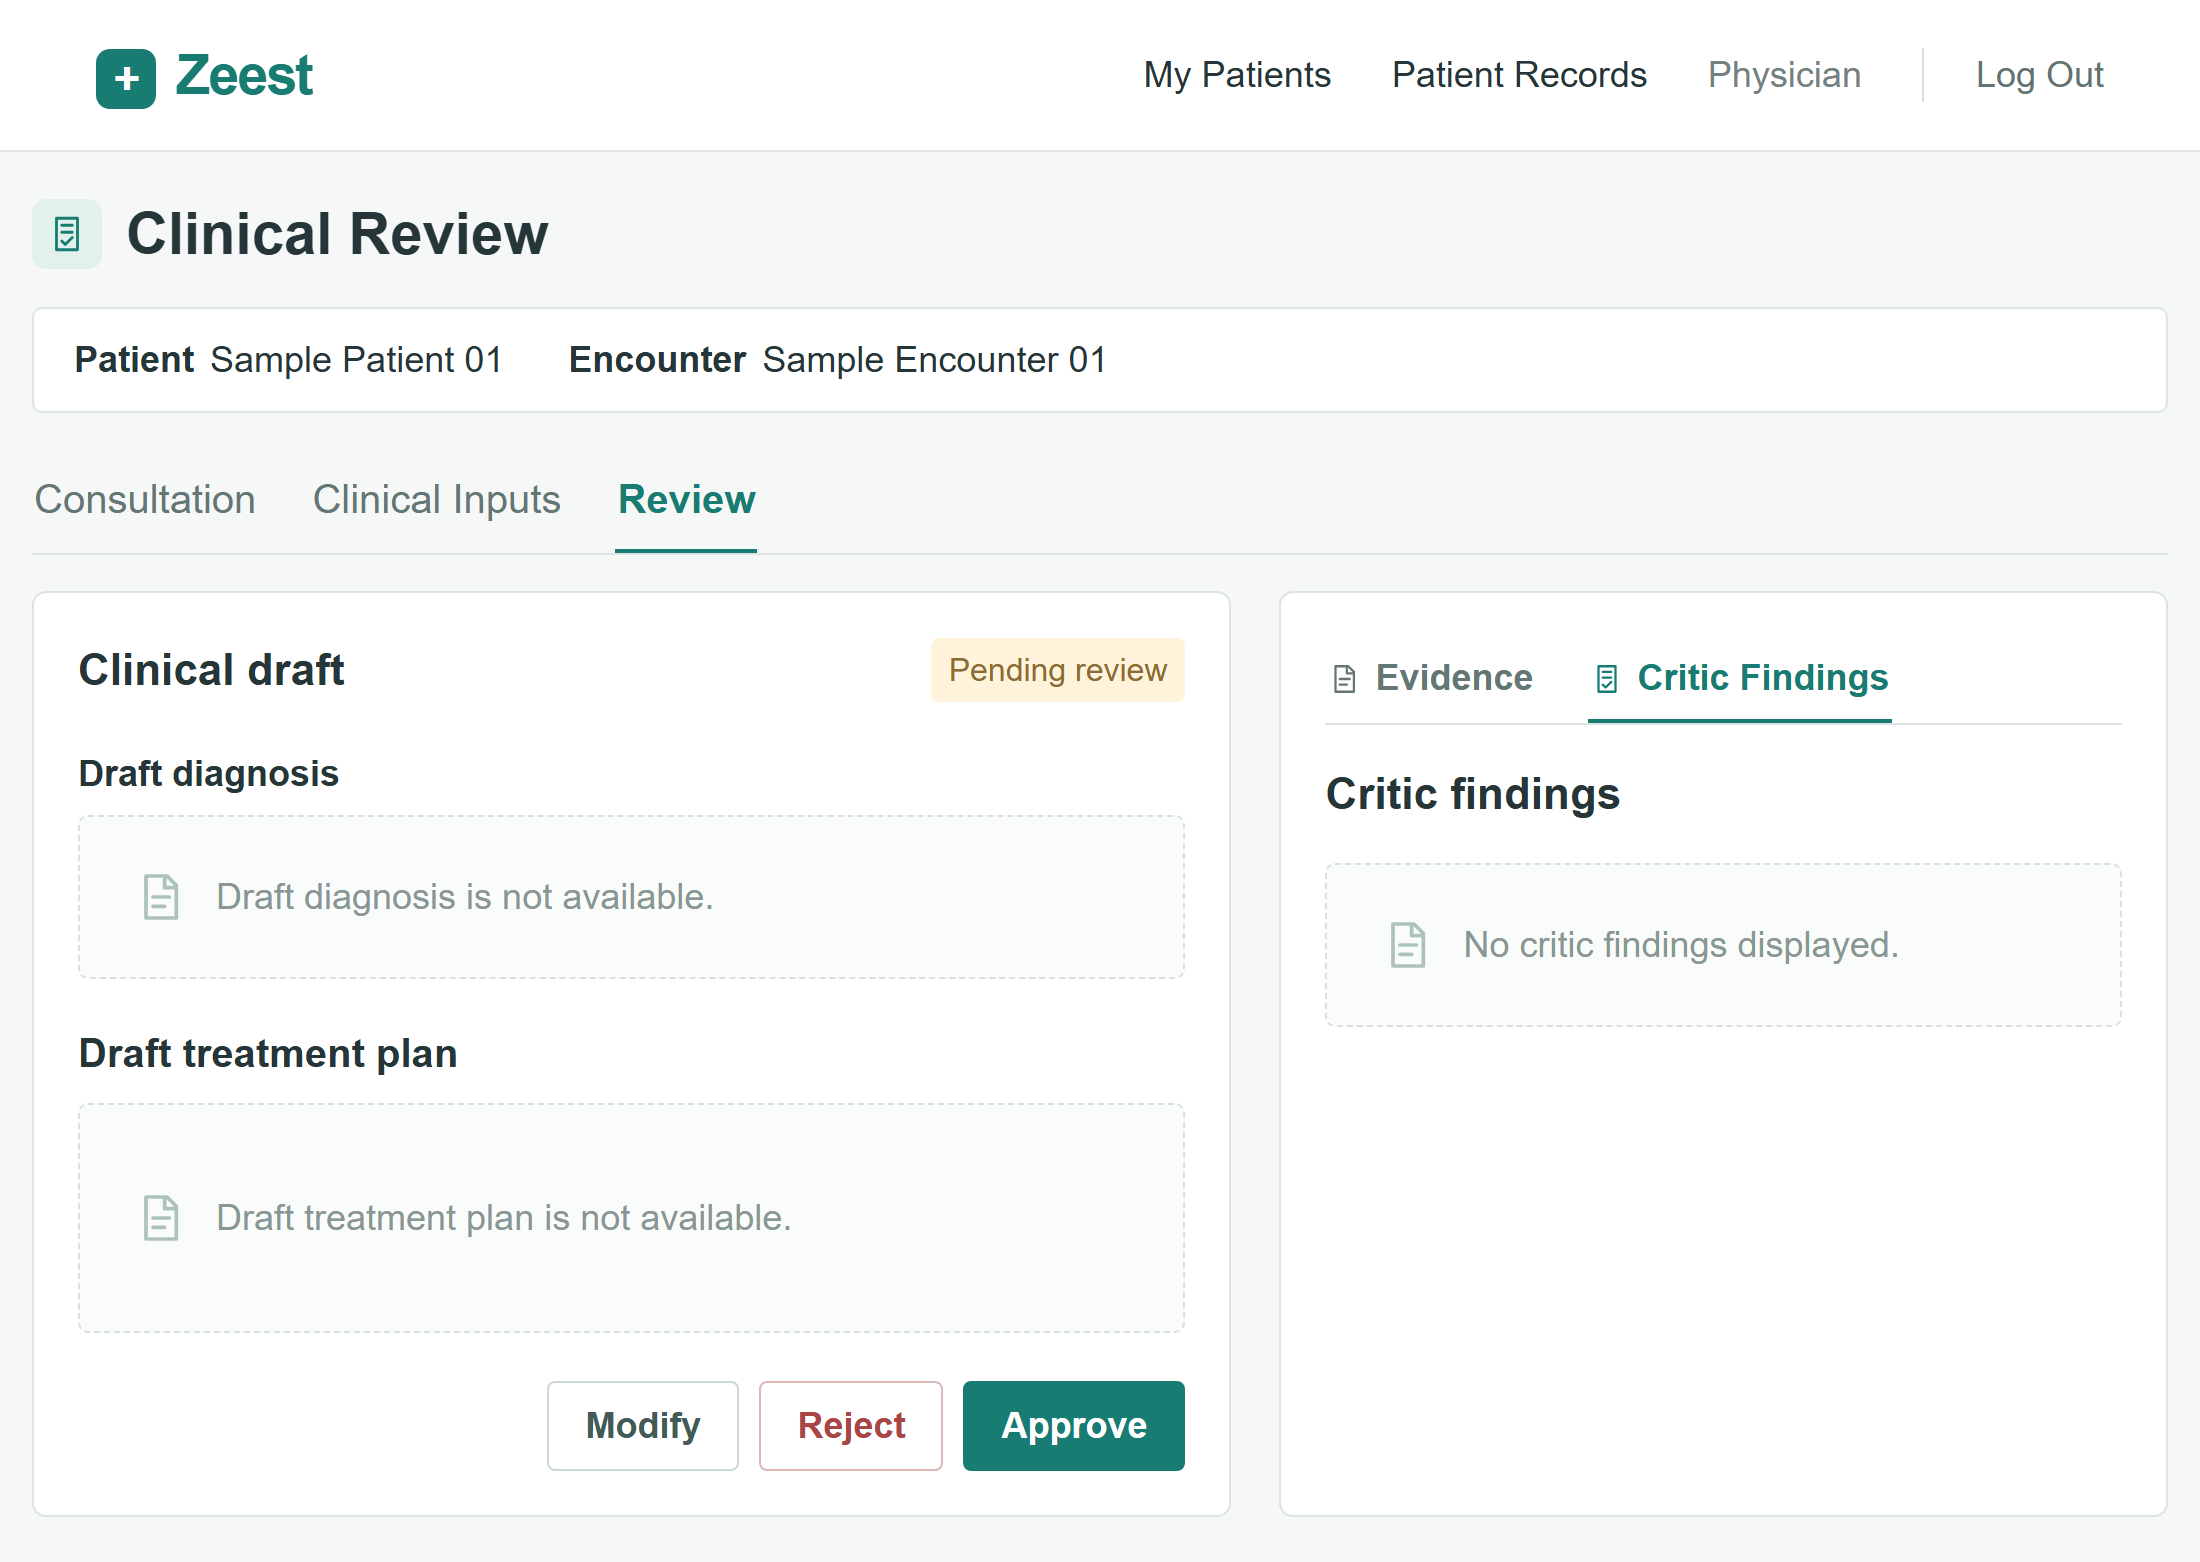
\includegraphics[width=0.96\textwidth,keepaspectratio]{Figures/kashaf_G10_critic.png}
\caption{Critic findings beside the clinical draft (Physician, UC15).}
\label{fig:kashaf:gui-critic}
\end{figure}

\begin{figure}[!htbp]
\centering
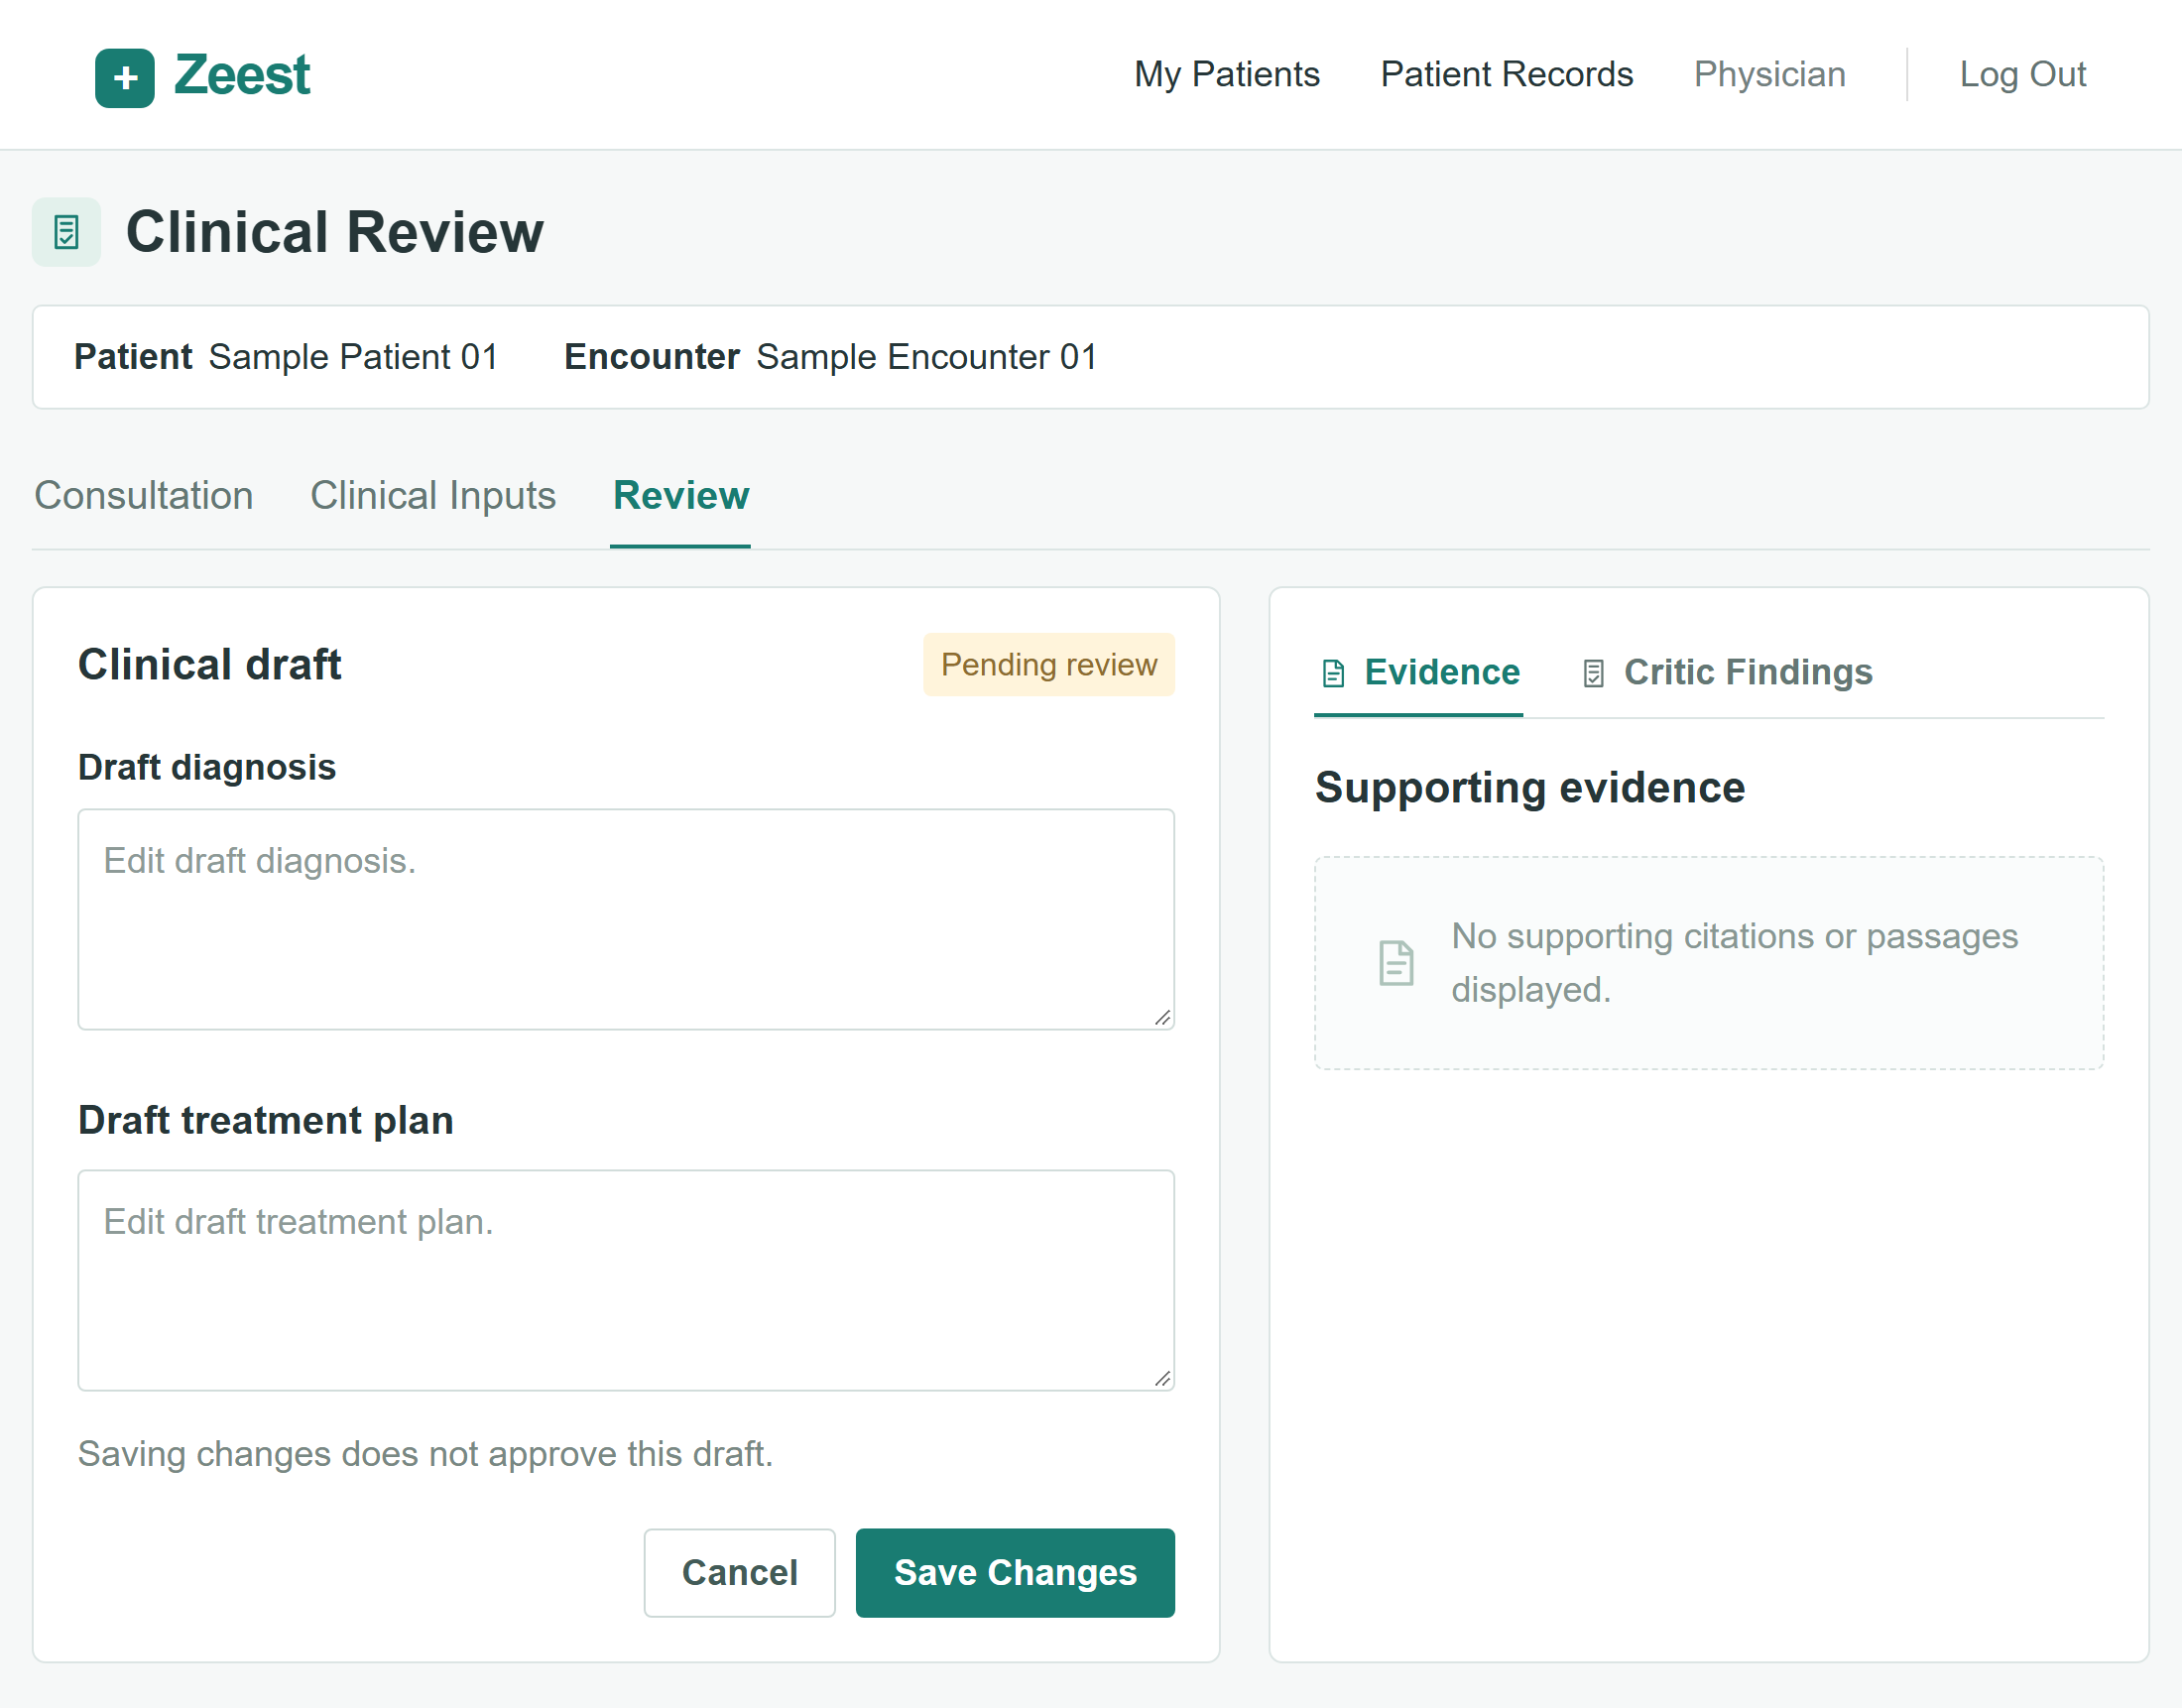
\includegraphics[width=0.96\textwidth,height=.88\textheight,keepaspectratio]{Figures/kashaf_G11_modify.png}
\caption{Draft revision editor and save controls (Physician, UC16).}
\label{fig:kashaf:gui-modify}

\centering
\end{figure}

\begin{figure}[!htbp]
\centering
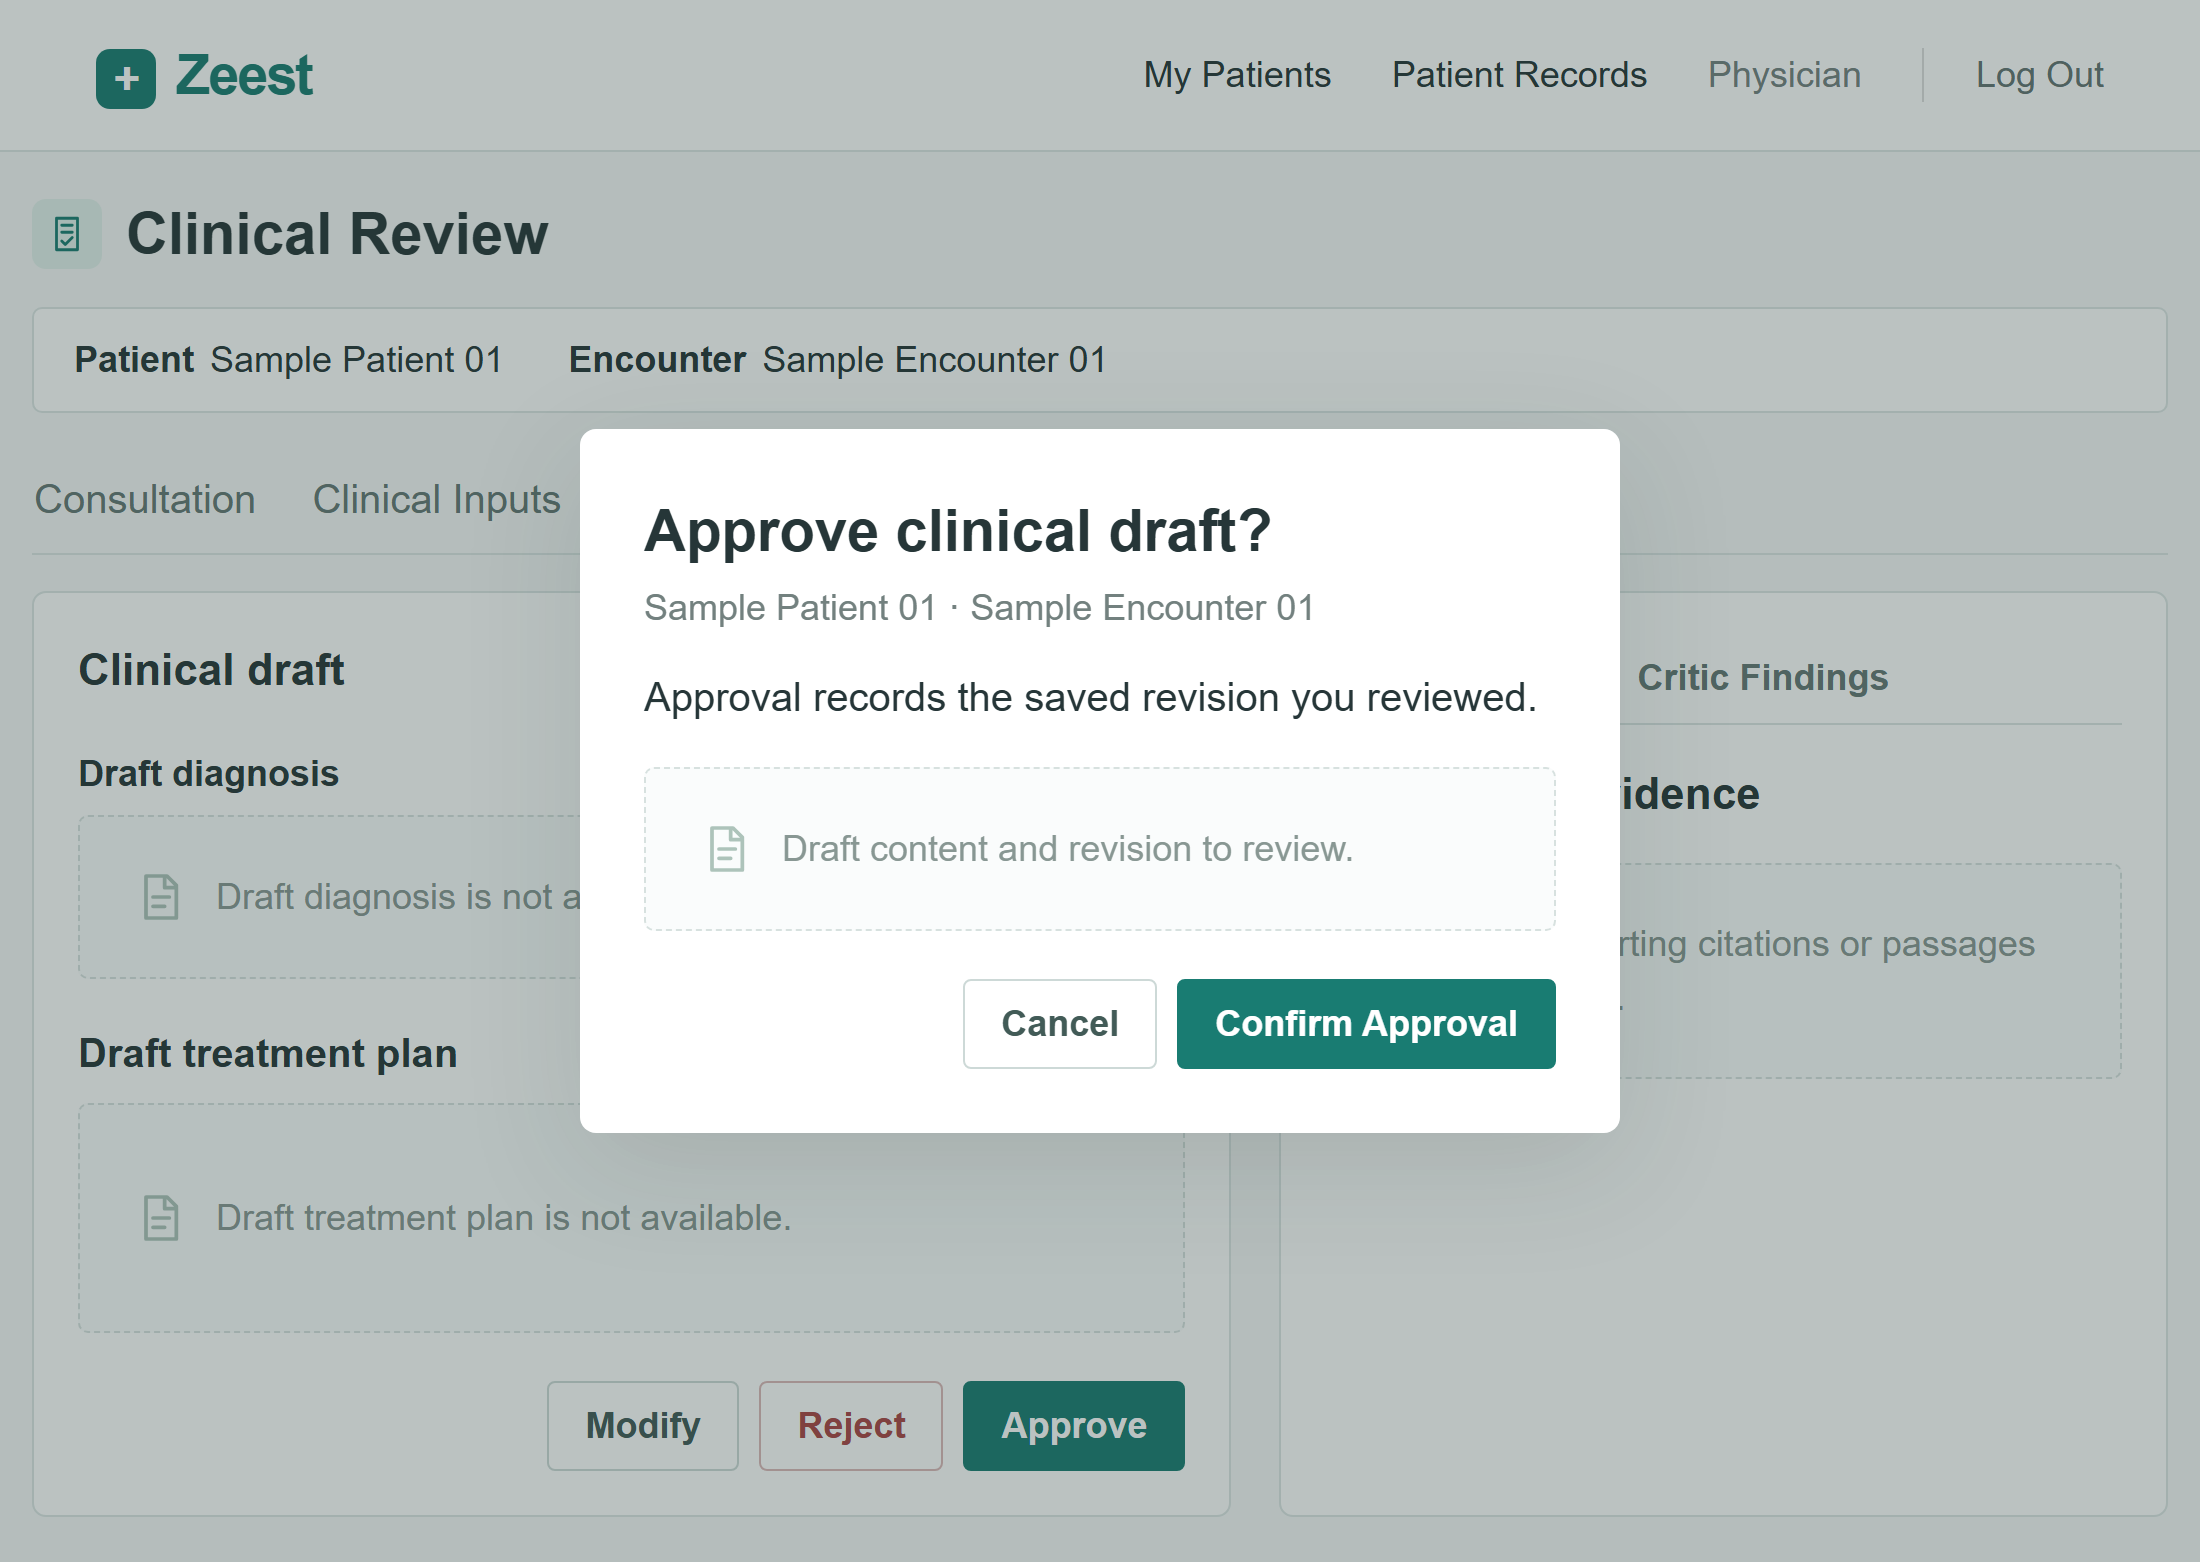
\includegraphics[width=0.96\textwidth,height=.88\textheight,keepaspectratio]{Figures/kashaf_G12_approve.png}
\caption{Confirmation dialog for explicit draft approval (Physician, UC17).}
\label{fig:kashaf:gui-approve}
\end{figure}

\begin{figure}[!htbp]
\centering
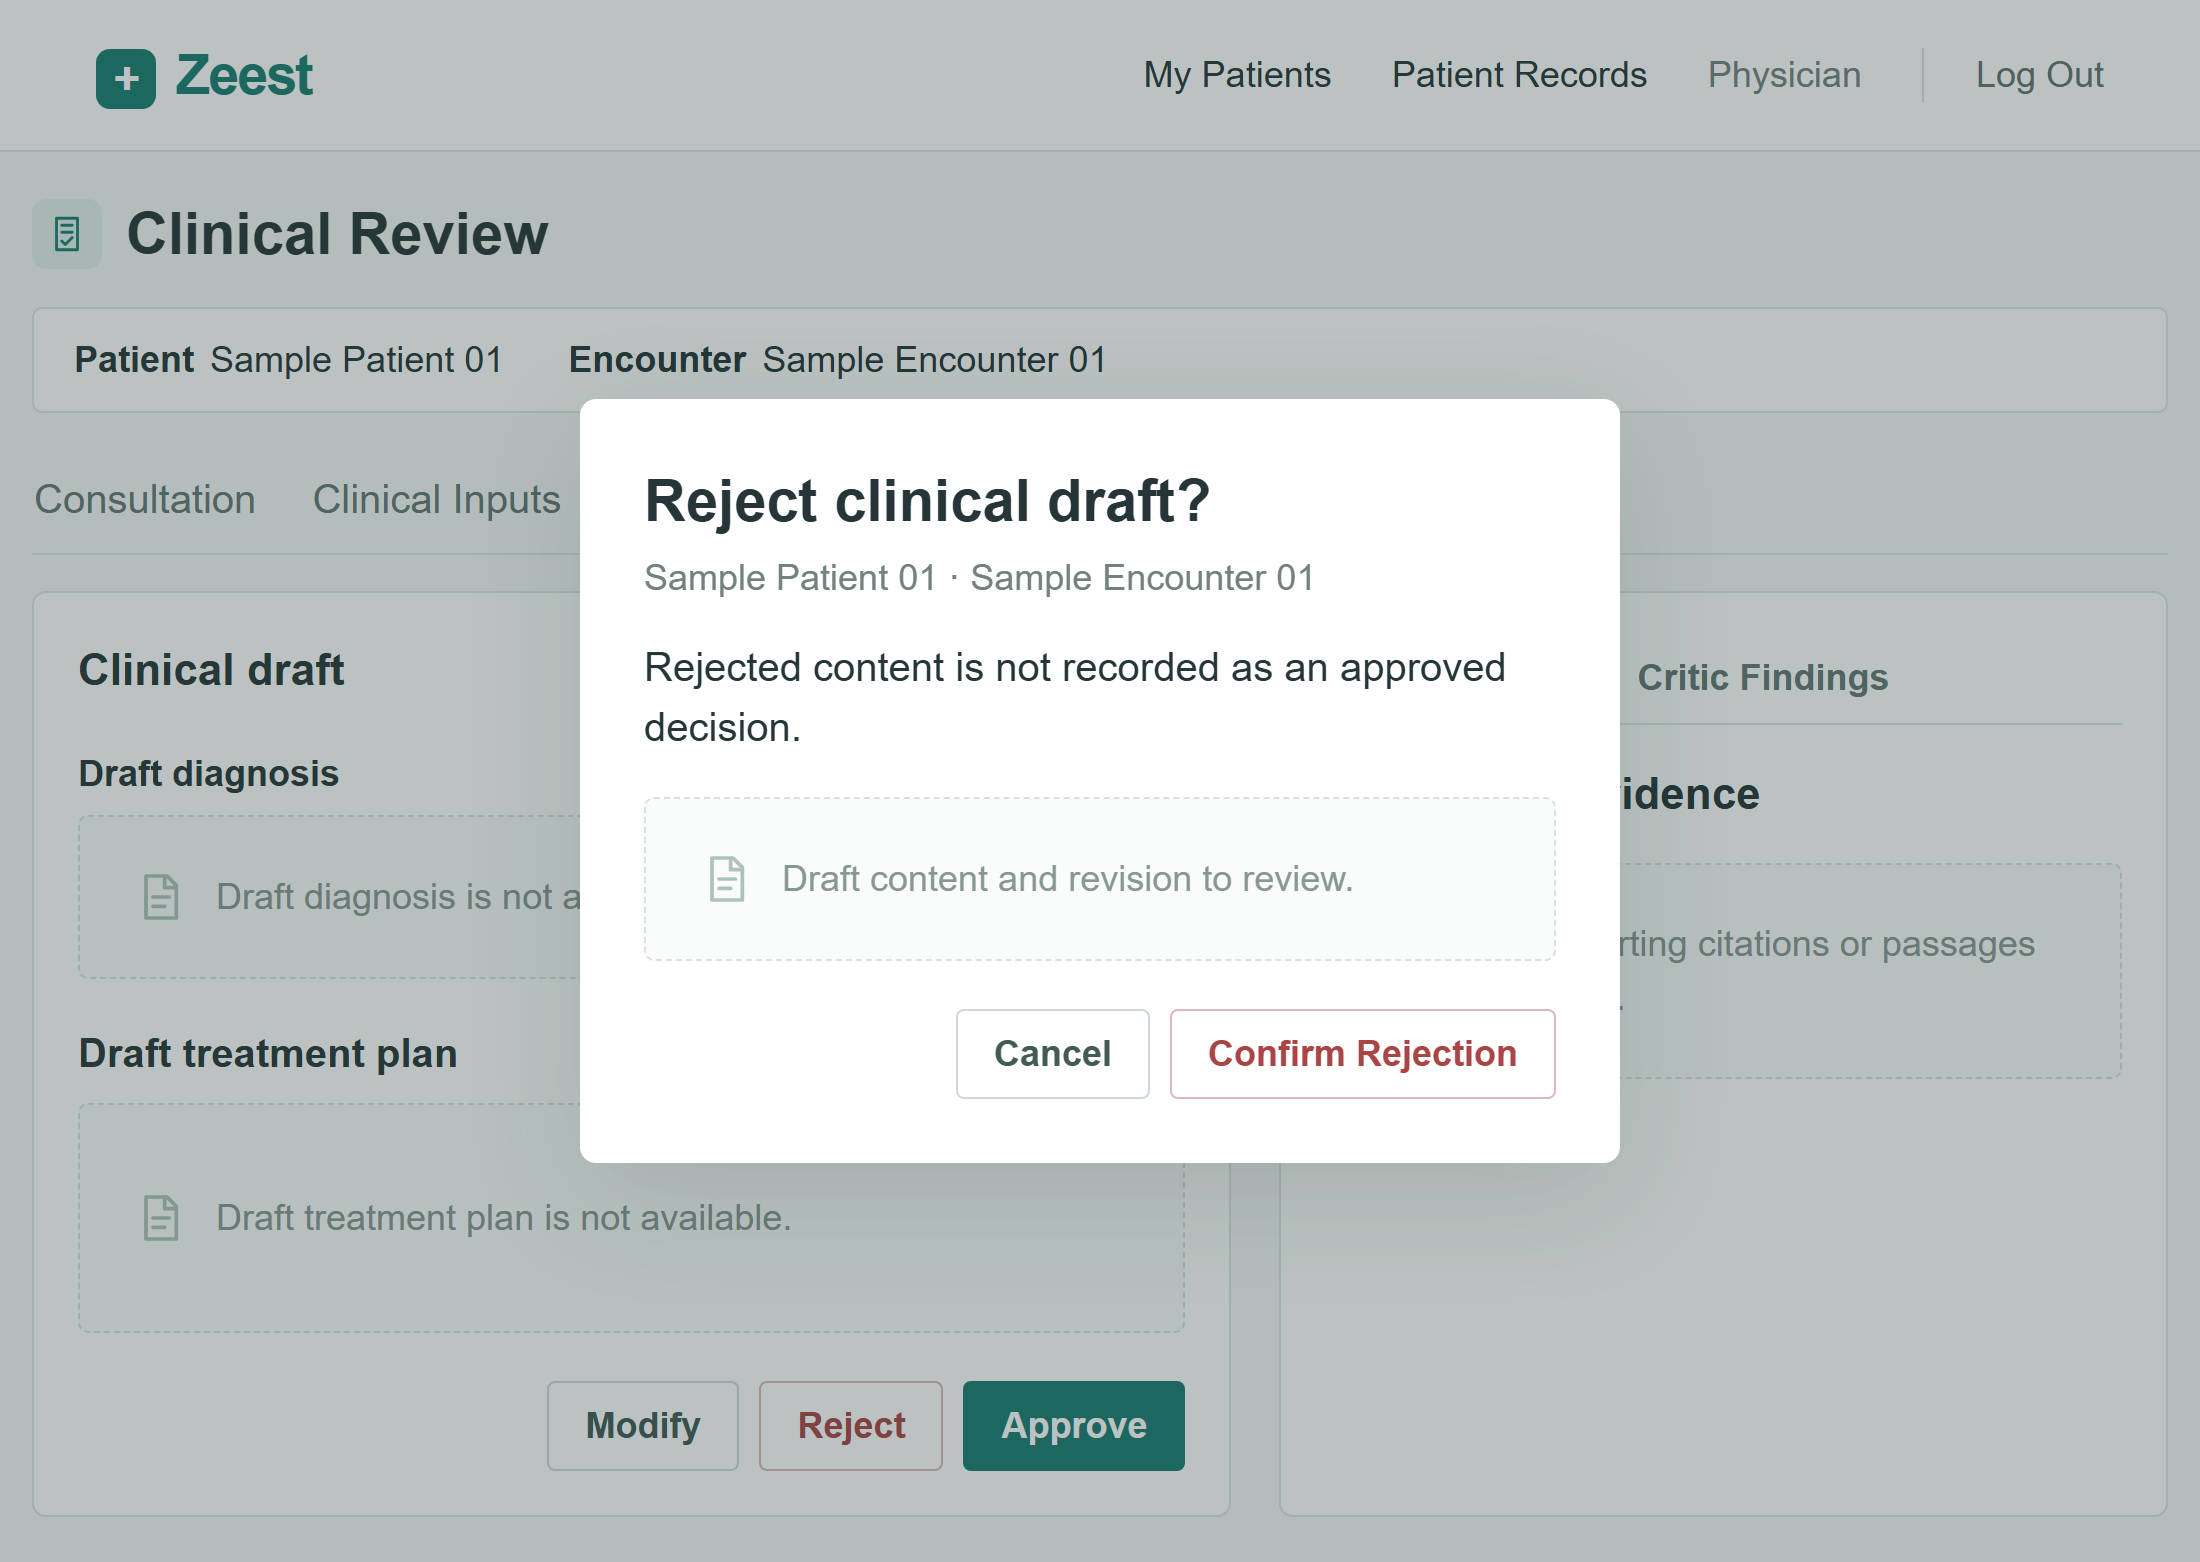
\includegraphics[width=0.96\textwidth,keepaspectratio]{Figures/kashaf_G13_reject.png}
\caption{Confirmation dialog for draft rejection (Physician, UC18).}
\label{fig:kashaf:gui-reject}

\centering
\vspace{10pt}
\centering
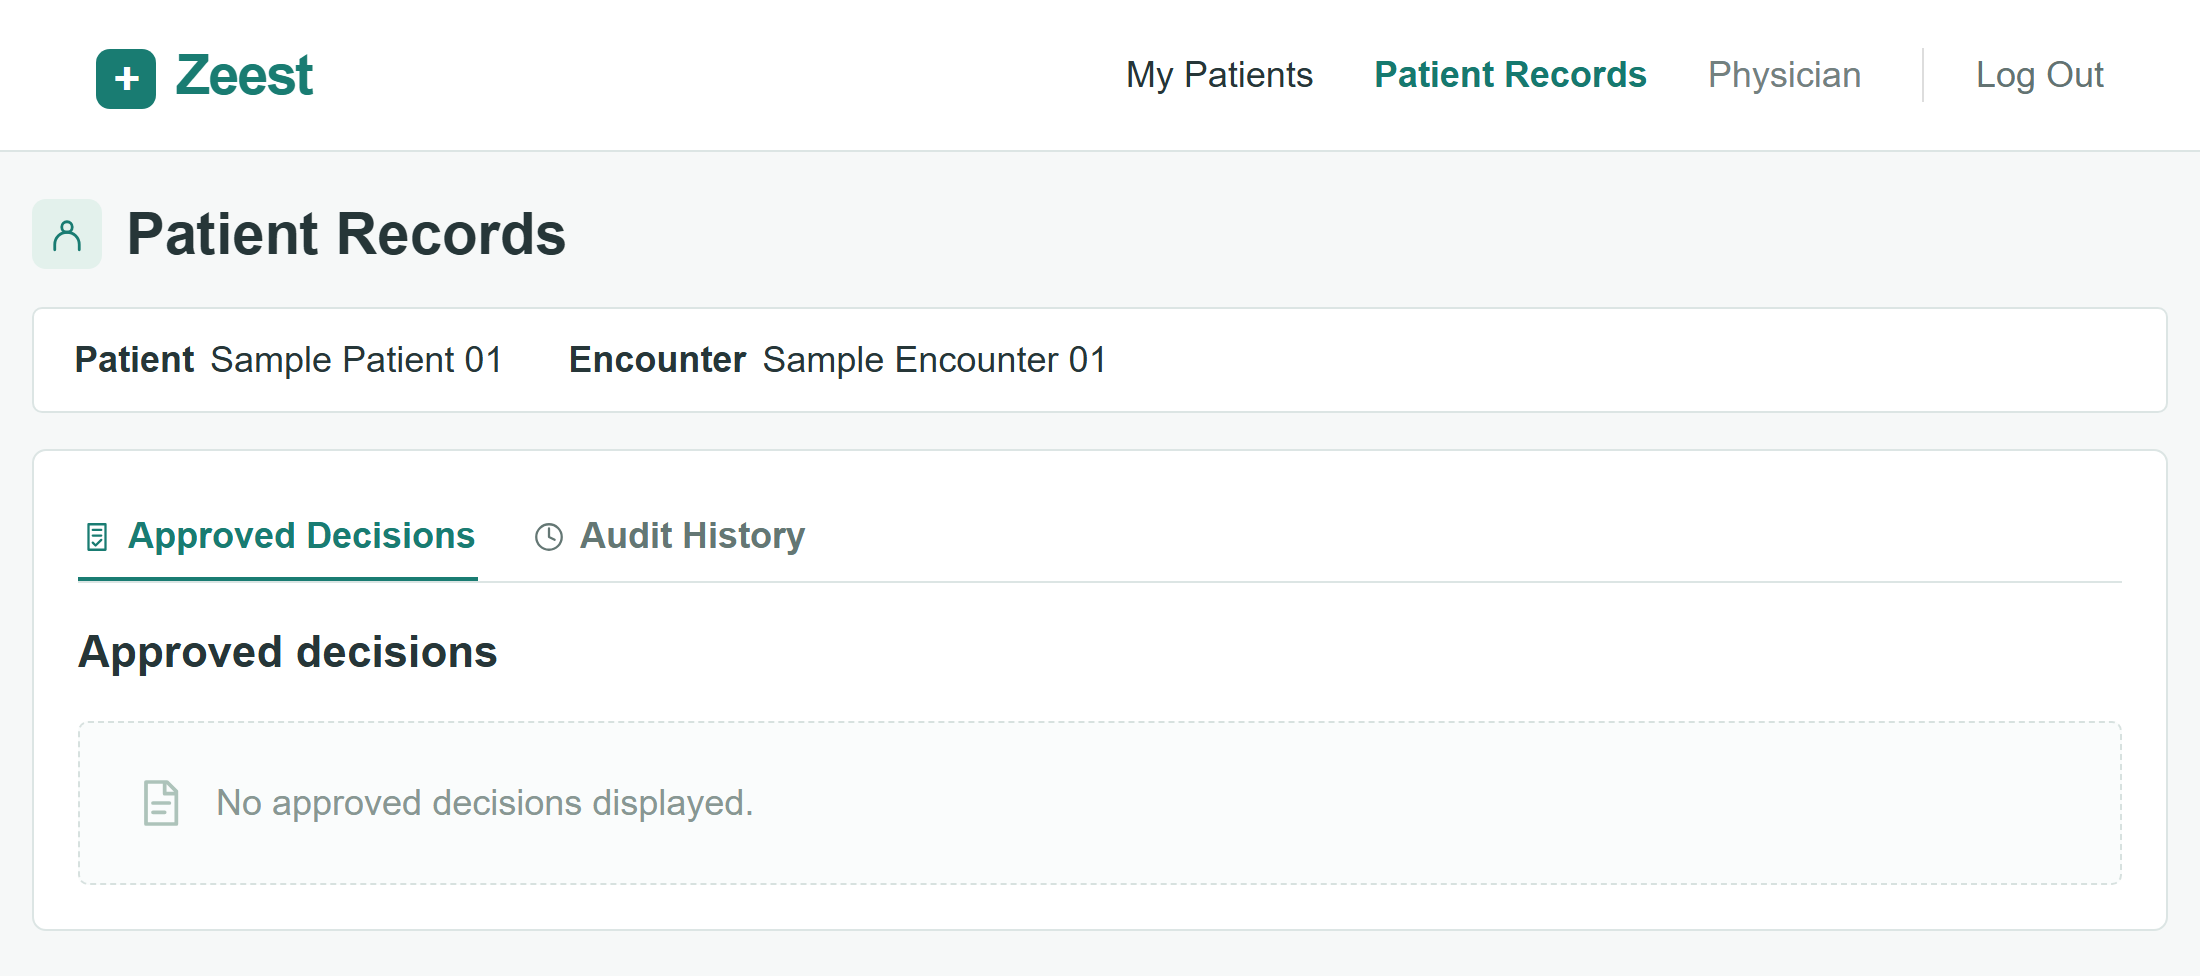
\includegraphics[width=0.96\textwidth,keepaspectratio]{Figures/kashaf_G14_decisions.png}
\caption{Selected encounter approved-decision view (Physician, UC19).}
\label{fig:kashaf:gui-decisions}
\end{figure}

\begin{figure}[!htbp]
\centering
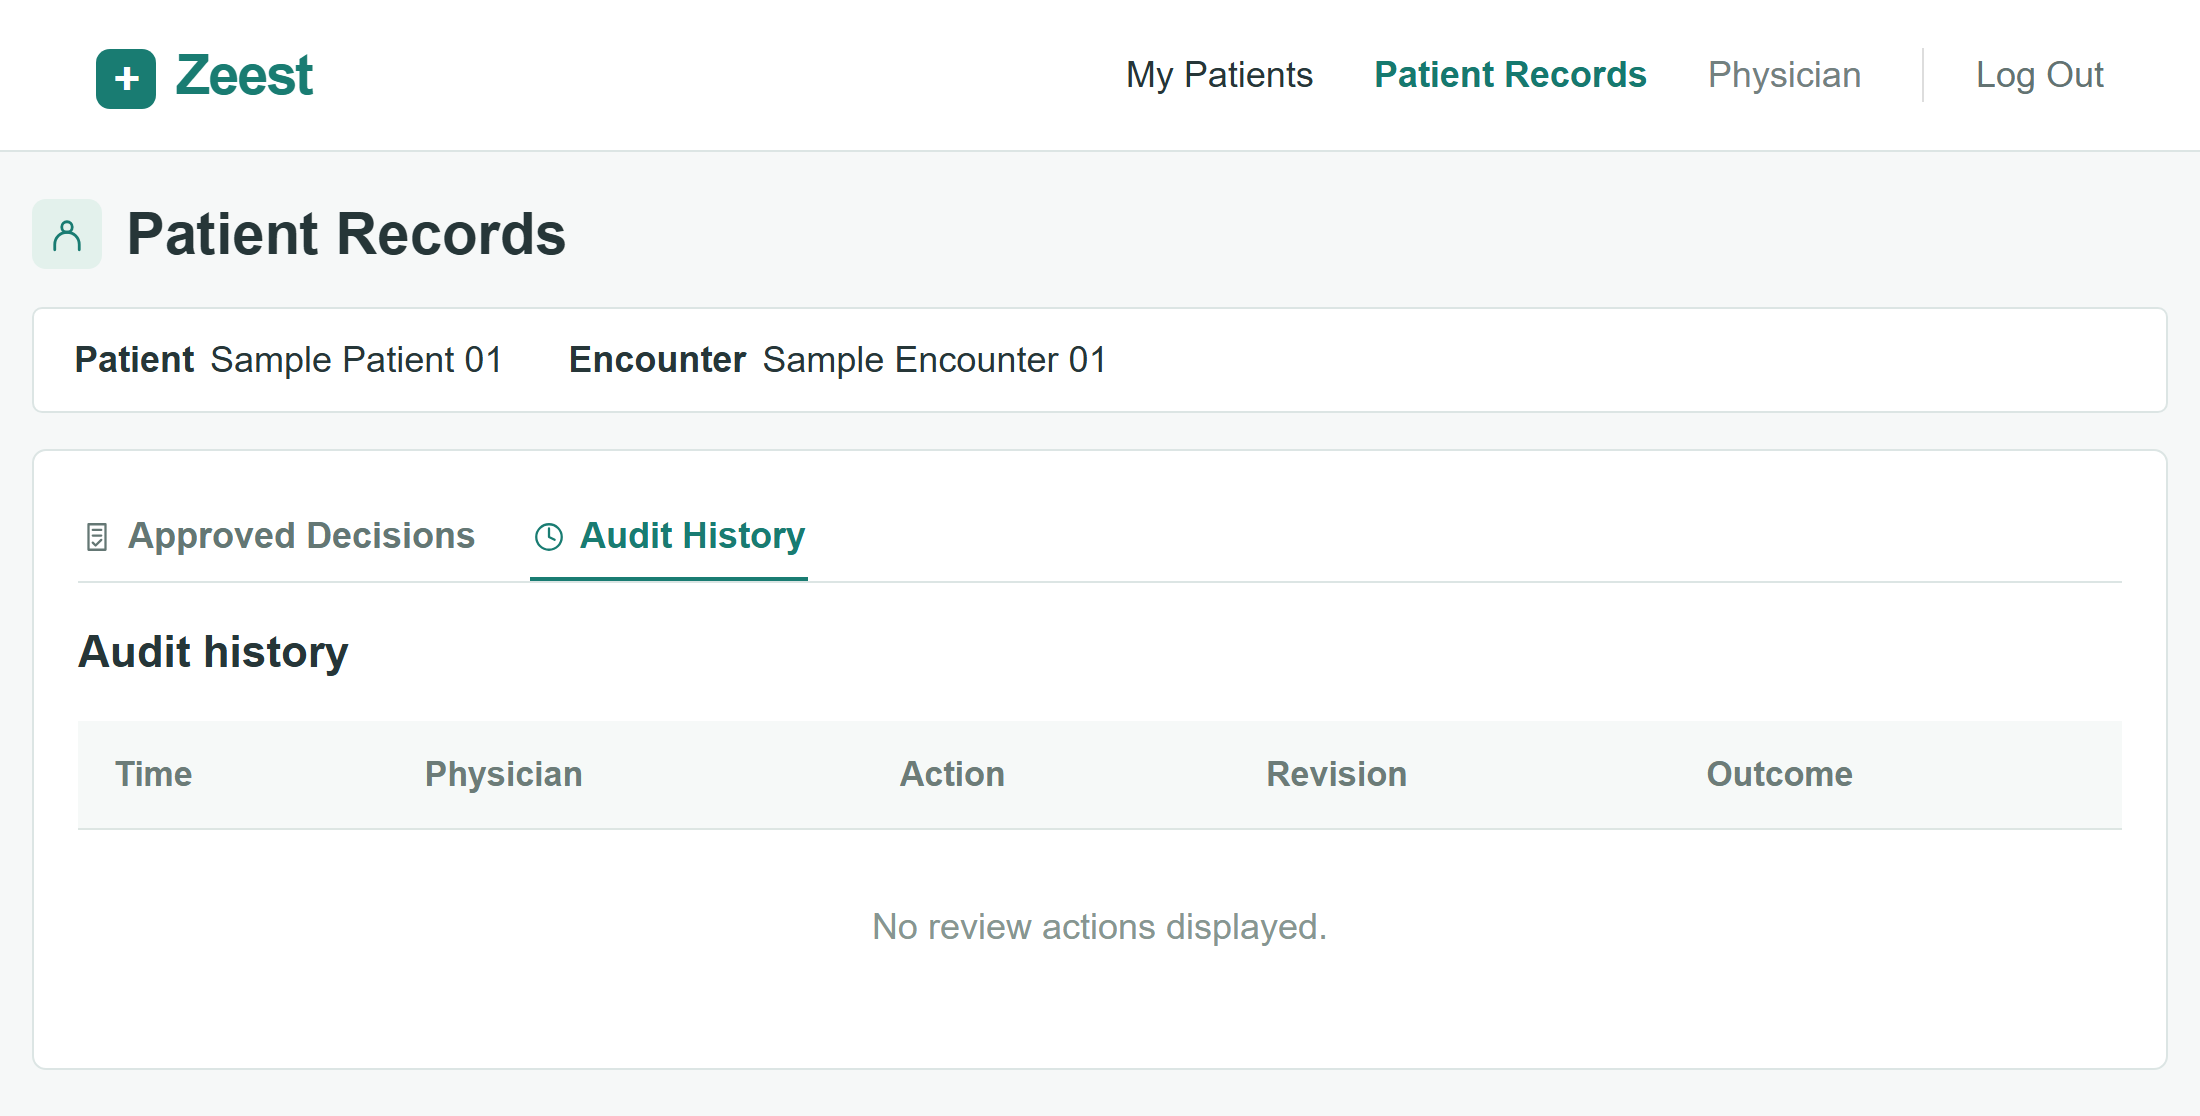
\includegraphics[width=0.96\textwidth,keepaspectratio]{Figures/kashaf_G15_audit.png}
\caption{Encounter review-action history table (Physician, UC20).}
\label{fig:kashaf:gui-audit}

\centering
\vspace{10pt}
\centering
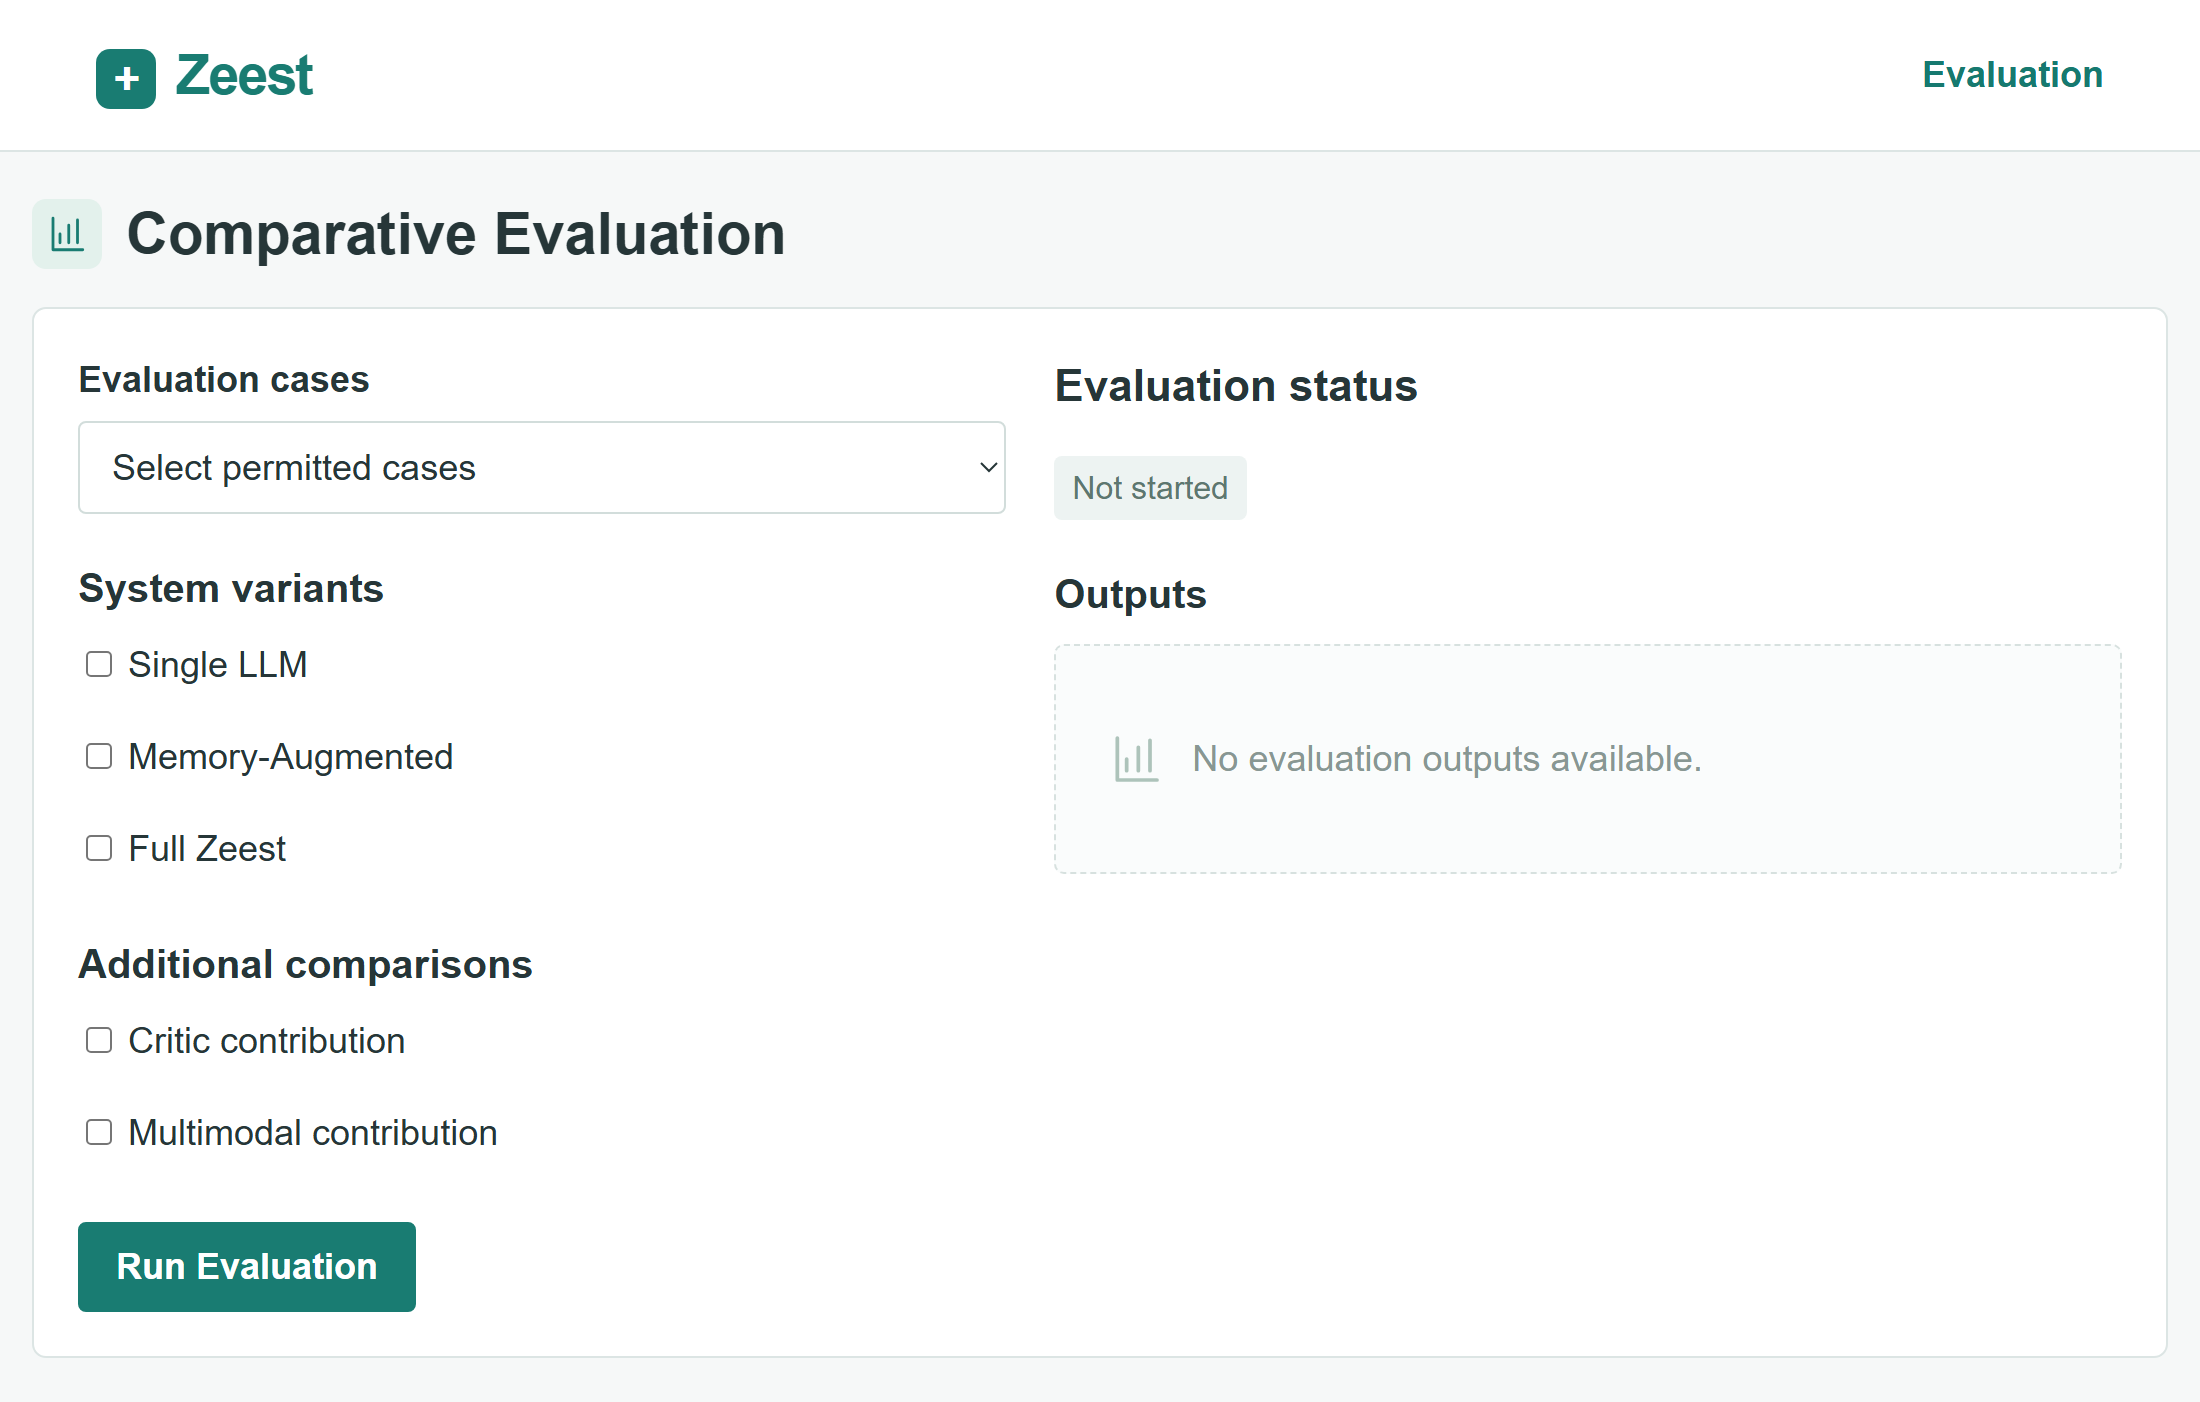
\includegraphics[width=0.96\textwidth,keepaspectratio]{Figures/kashaf_G16_evaluation.png}
\caption{Case, variant and run controls for comparative evaluation (Research team, UC22).}
\label{fig:kashaf:gui-evaluation}
\end{figure}


\section{Database Design}

The logical design separates physician accounts, patient ownership, clinical information, generated drafts and accepted decisions. Each patient has one responsible physician, and encounters inherit that ownership through the patient. Clinical case inputs retain saved revisions, allowing findings and draft preparation to identify their exact source content. Draft revisions keep diagnosis and treatment text distinct from approval actions and accepted decisions. Retrieved evidence and critic reviews refer to the assessed revision. Semantic representations originate from an input revision or an approved decision. Separate evaluation records connect permitted cases, run settings and recorded outputs. These relationships preserve continuity, source traceability and physician authority across the defined clinical workflow. The schema is a logical design rather than an implemented database. Patient ownership and revision consistency require explicit validation alongside foreign keys. Model-dependent vector dimensions remain configuration choices, and evaluation outputs represent records to be populated after actual runs rather than supplied numerical findings.

\subsection{ER Diagram}

Figure~\ref{fig:kashaf:er} presents the complete conceptual model with entities, relationship diamonds and attribute ovals together. Dashed regions group accounts and clinical information, drafts and supporting evidence, physician review and memory, and comparative evaluation. Blue rectangles identify entities, green ovals identify attributes, and amber diamonds identify named relationships. Primary keys are underlined and foreign keys are marked FK. Cardinalities express ownership and record associations, while revision keys preserve the exact content used or reviewed. Figures~\ref{fig:kashaf:er-clinical}, \ref{fig:kashaf:er-drafts}, \ref{fig:kashaf:er-review} and~\ref{fig:kashaf:er-evaluation} enlarge the same regions; cross-region relationships remain visible in the complete model. The grouped enlargements retain the same entity and relationship names as the overview, allowing attributes and cardinalities to be read at print size. Login and registration are account operations rather than separate persistent clinical entities. Evaluation links remain separate from clinical decisions, so a comparative output cannot become an approved patient record merely because it was saved. Region enlargements preserve the same underlying schema.

\begin{figure}[!htbp]
\centering
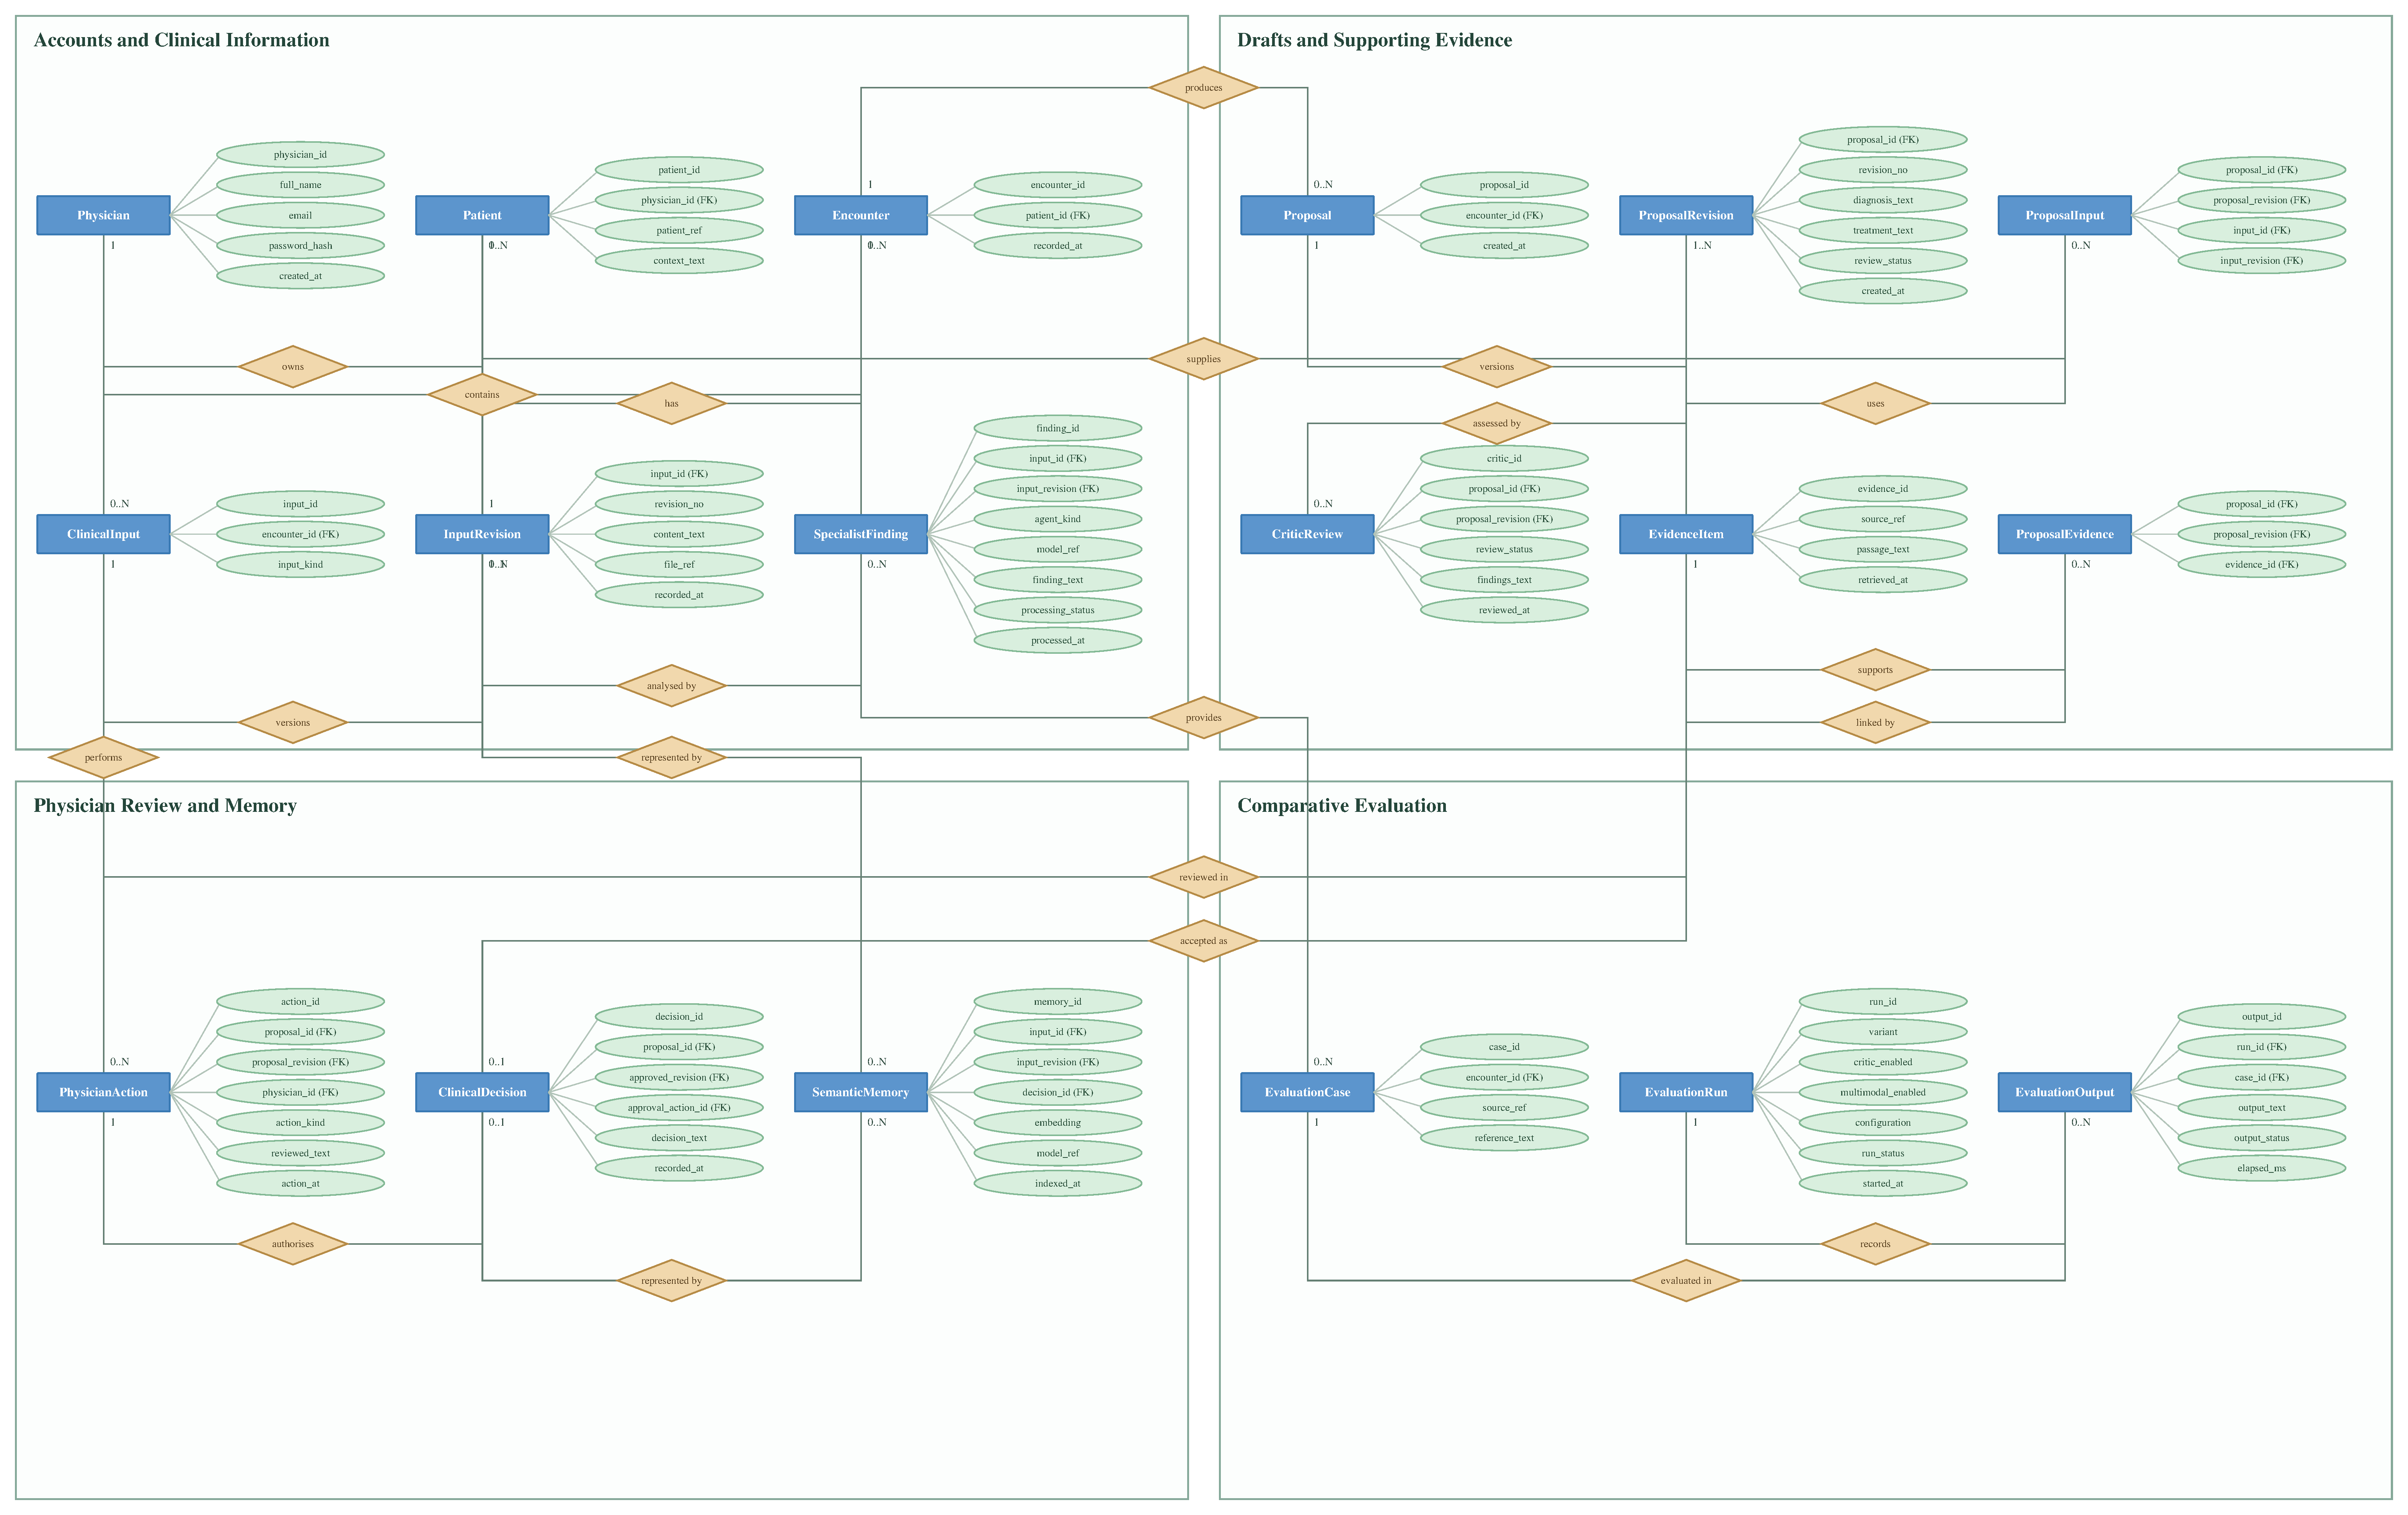
\includegraphics[width=\textwidth,height=0.80\textheight,keepaspectratio]{Figures/kashaf_D03_conceptual_combined.pdf}
\caption{Complete grouped conceptual ER model with entity, attribute and relationship symbols.}
\label{fig:kashaf:er}
\end{figure}

\begin{figure}[!htbp]
\centering
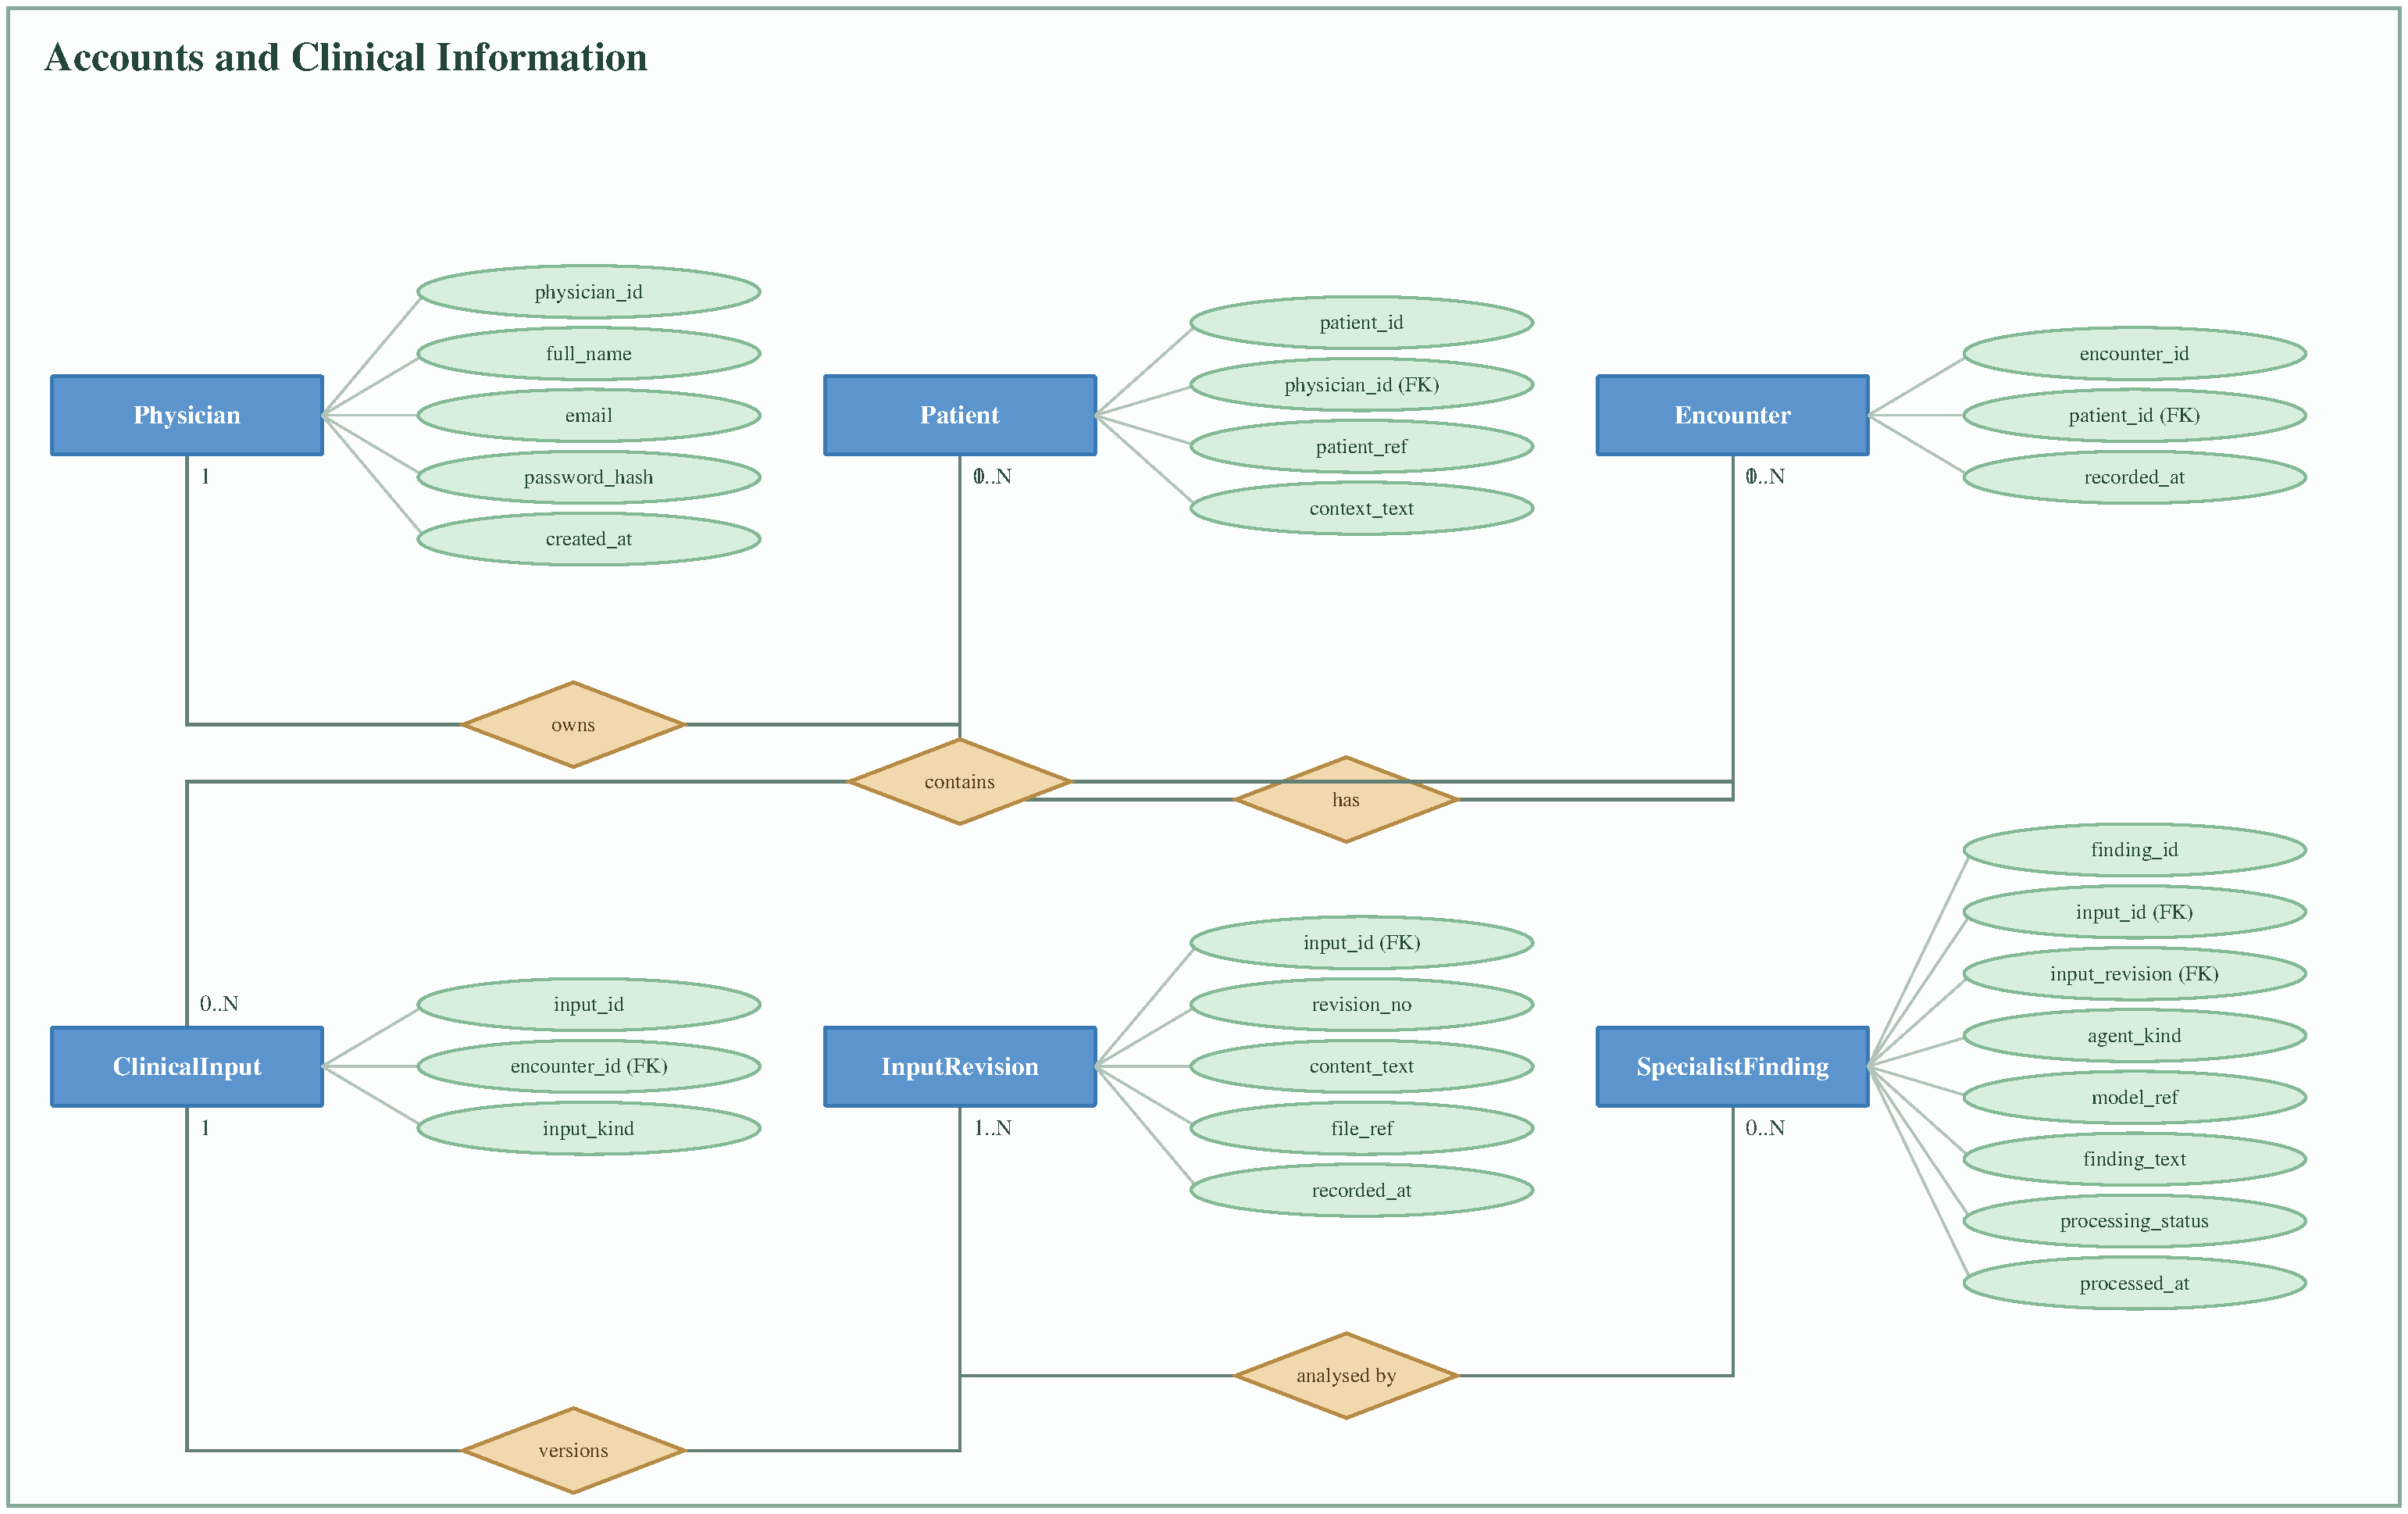
\includegraphics[width=\textwidth,height=0.80\textheight,keepaspectratio]{Figures/kashaf_D03_combined_clinical.pdf}
\caption{Accounts and clinical sources with attributes and relationship cardinalities.}
\label{fig:kashaf:er-clinical}
\end{figure}

\begin{figure}[!htbp]
\centering
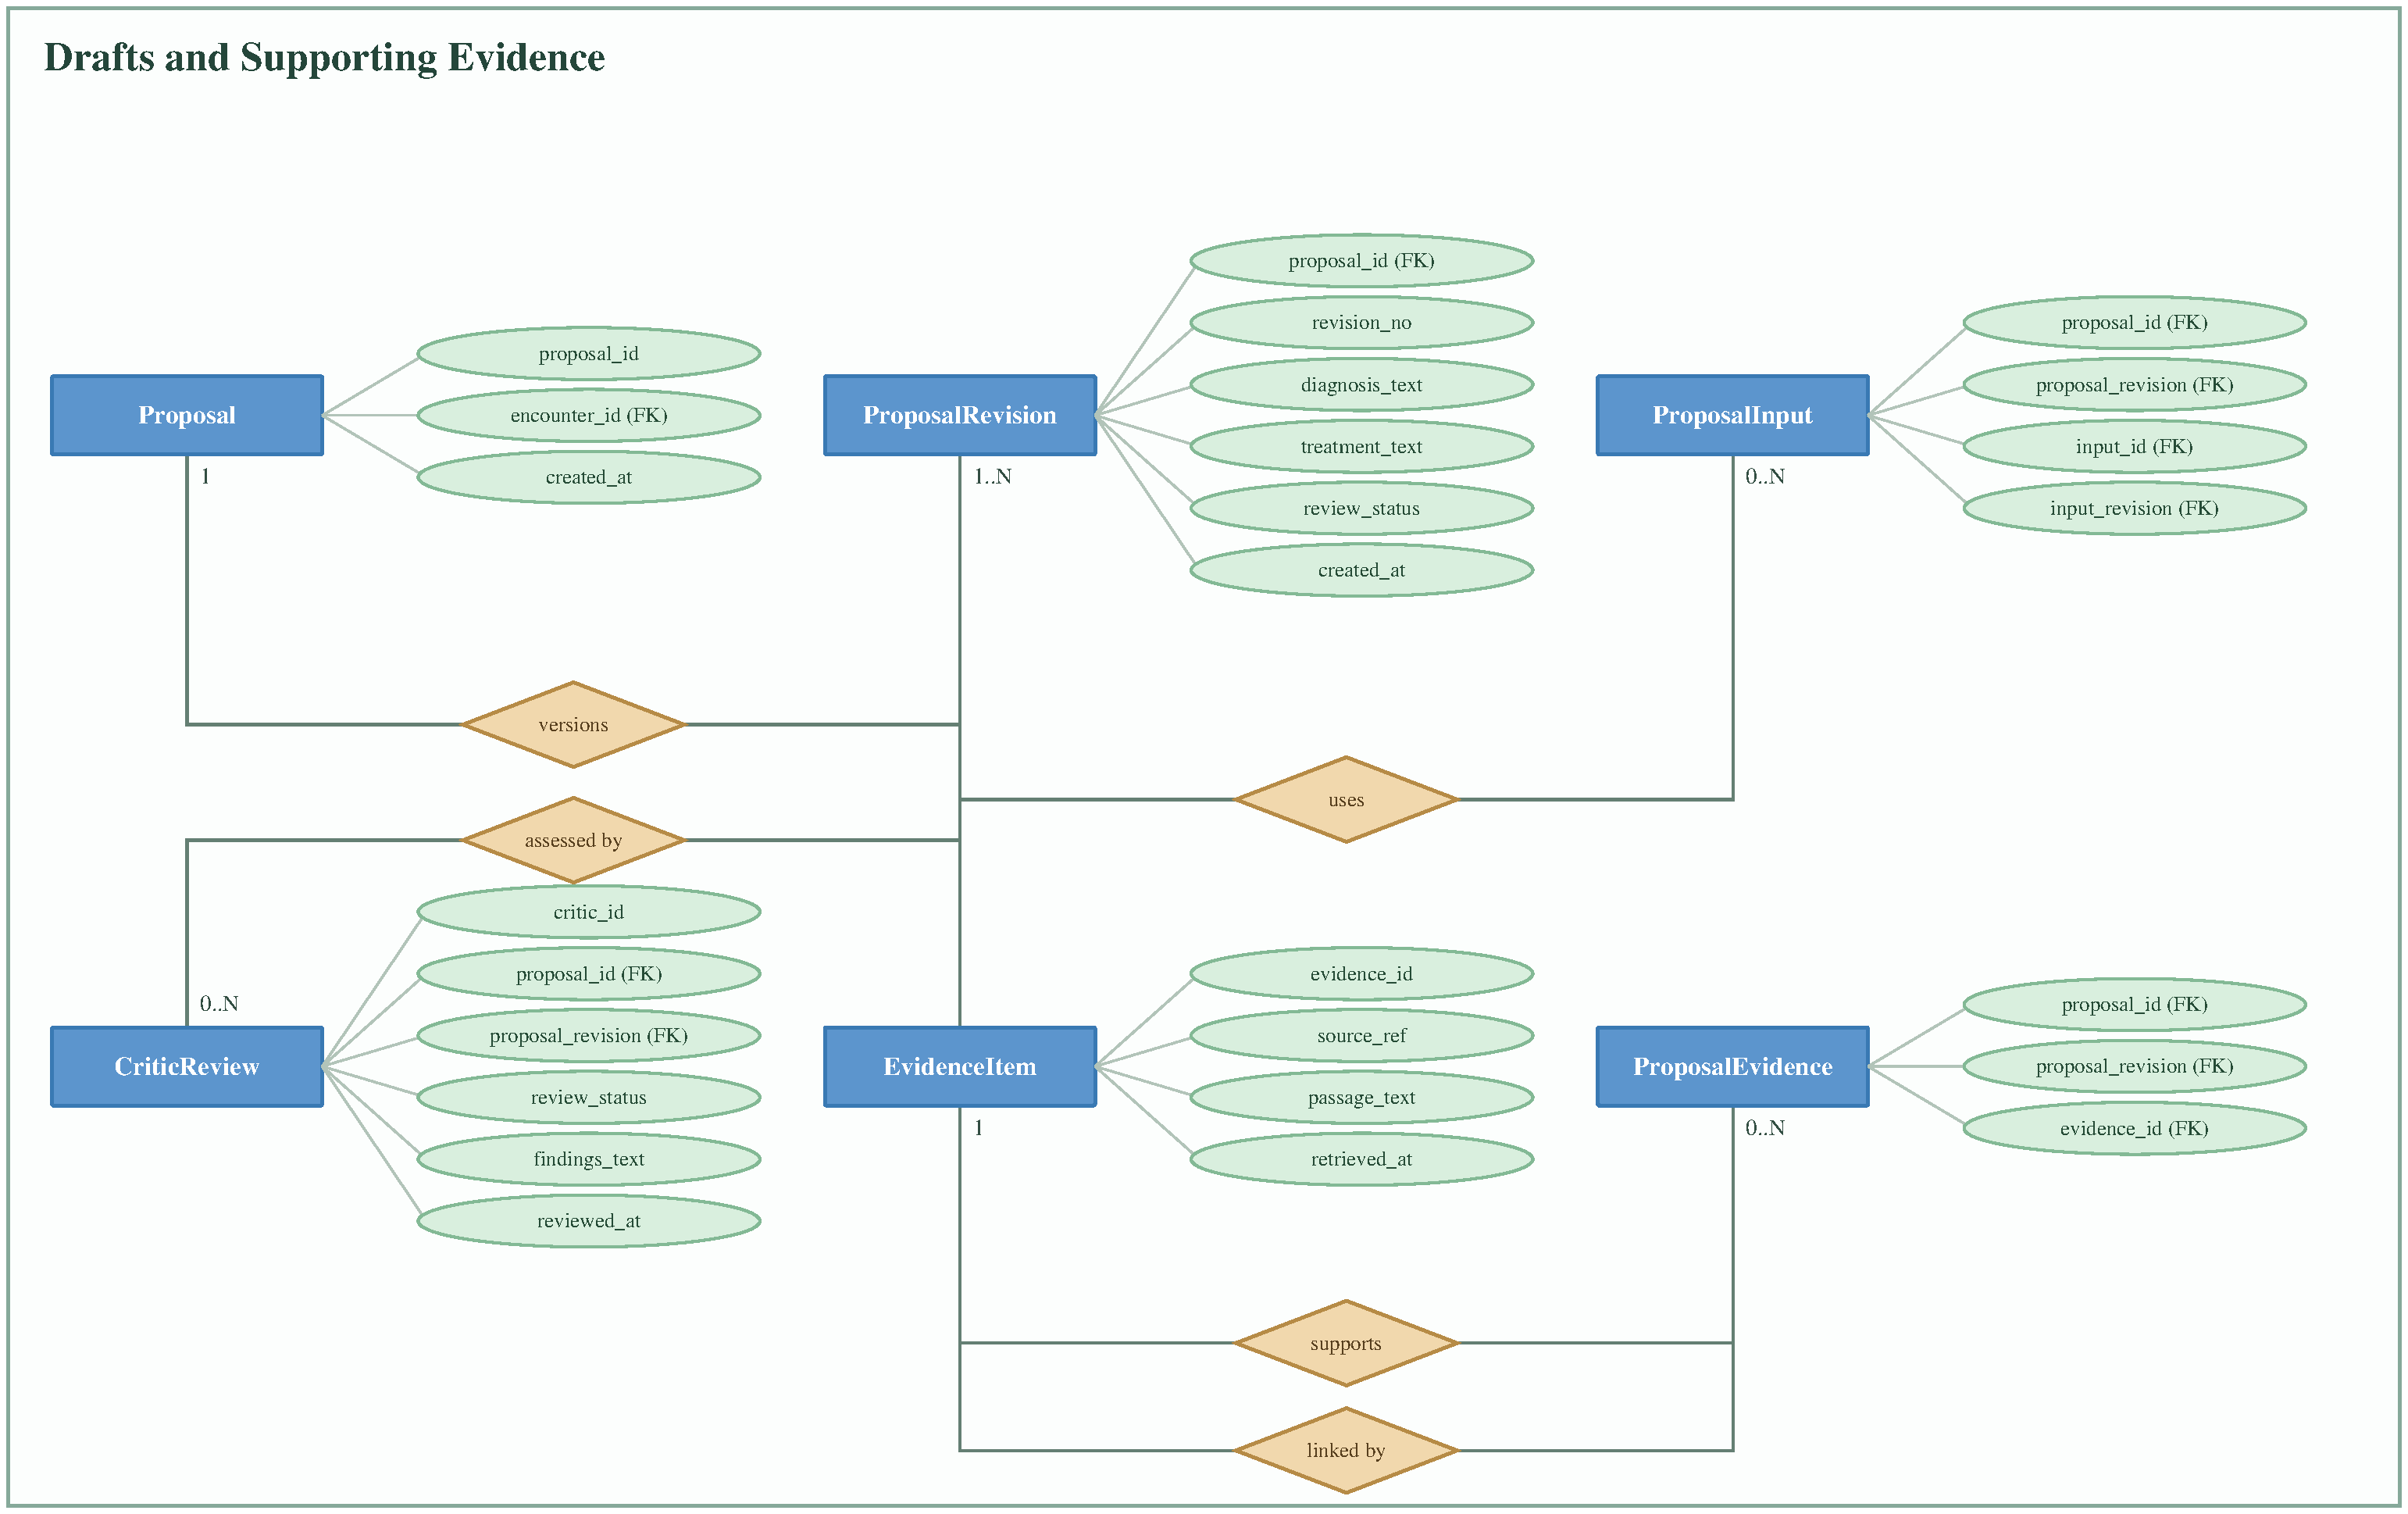
\includegraphics[width=\textwidth,height=0.80\textheight,keepaspectratio]{Figures/kashaf_D03_combined_drafts.pdf}
\caption{Draft revisions, evidence and critic review with attributes and relationships.}
\label{fig:kashaf:er-drafts}
\end{figure}

\begin{figure}[!htbp]
\centering
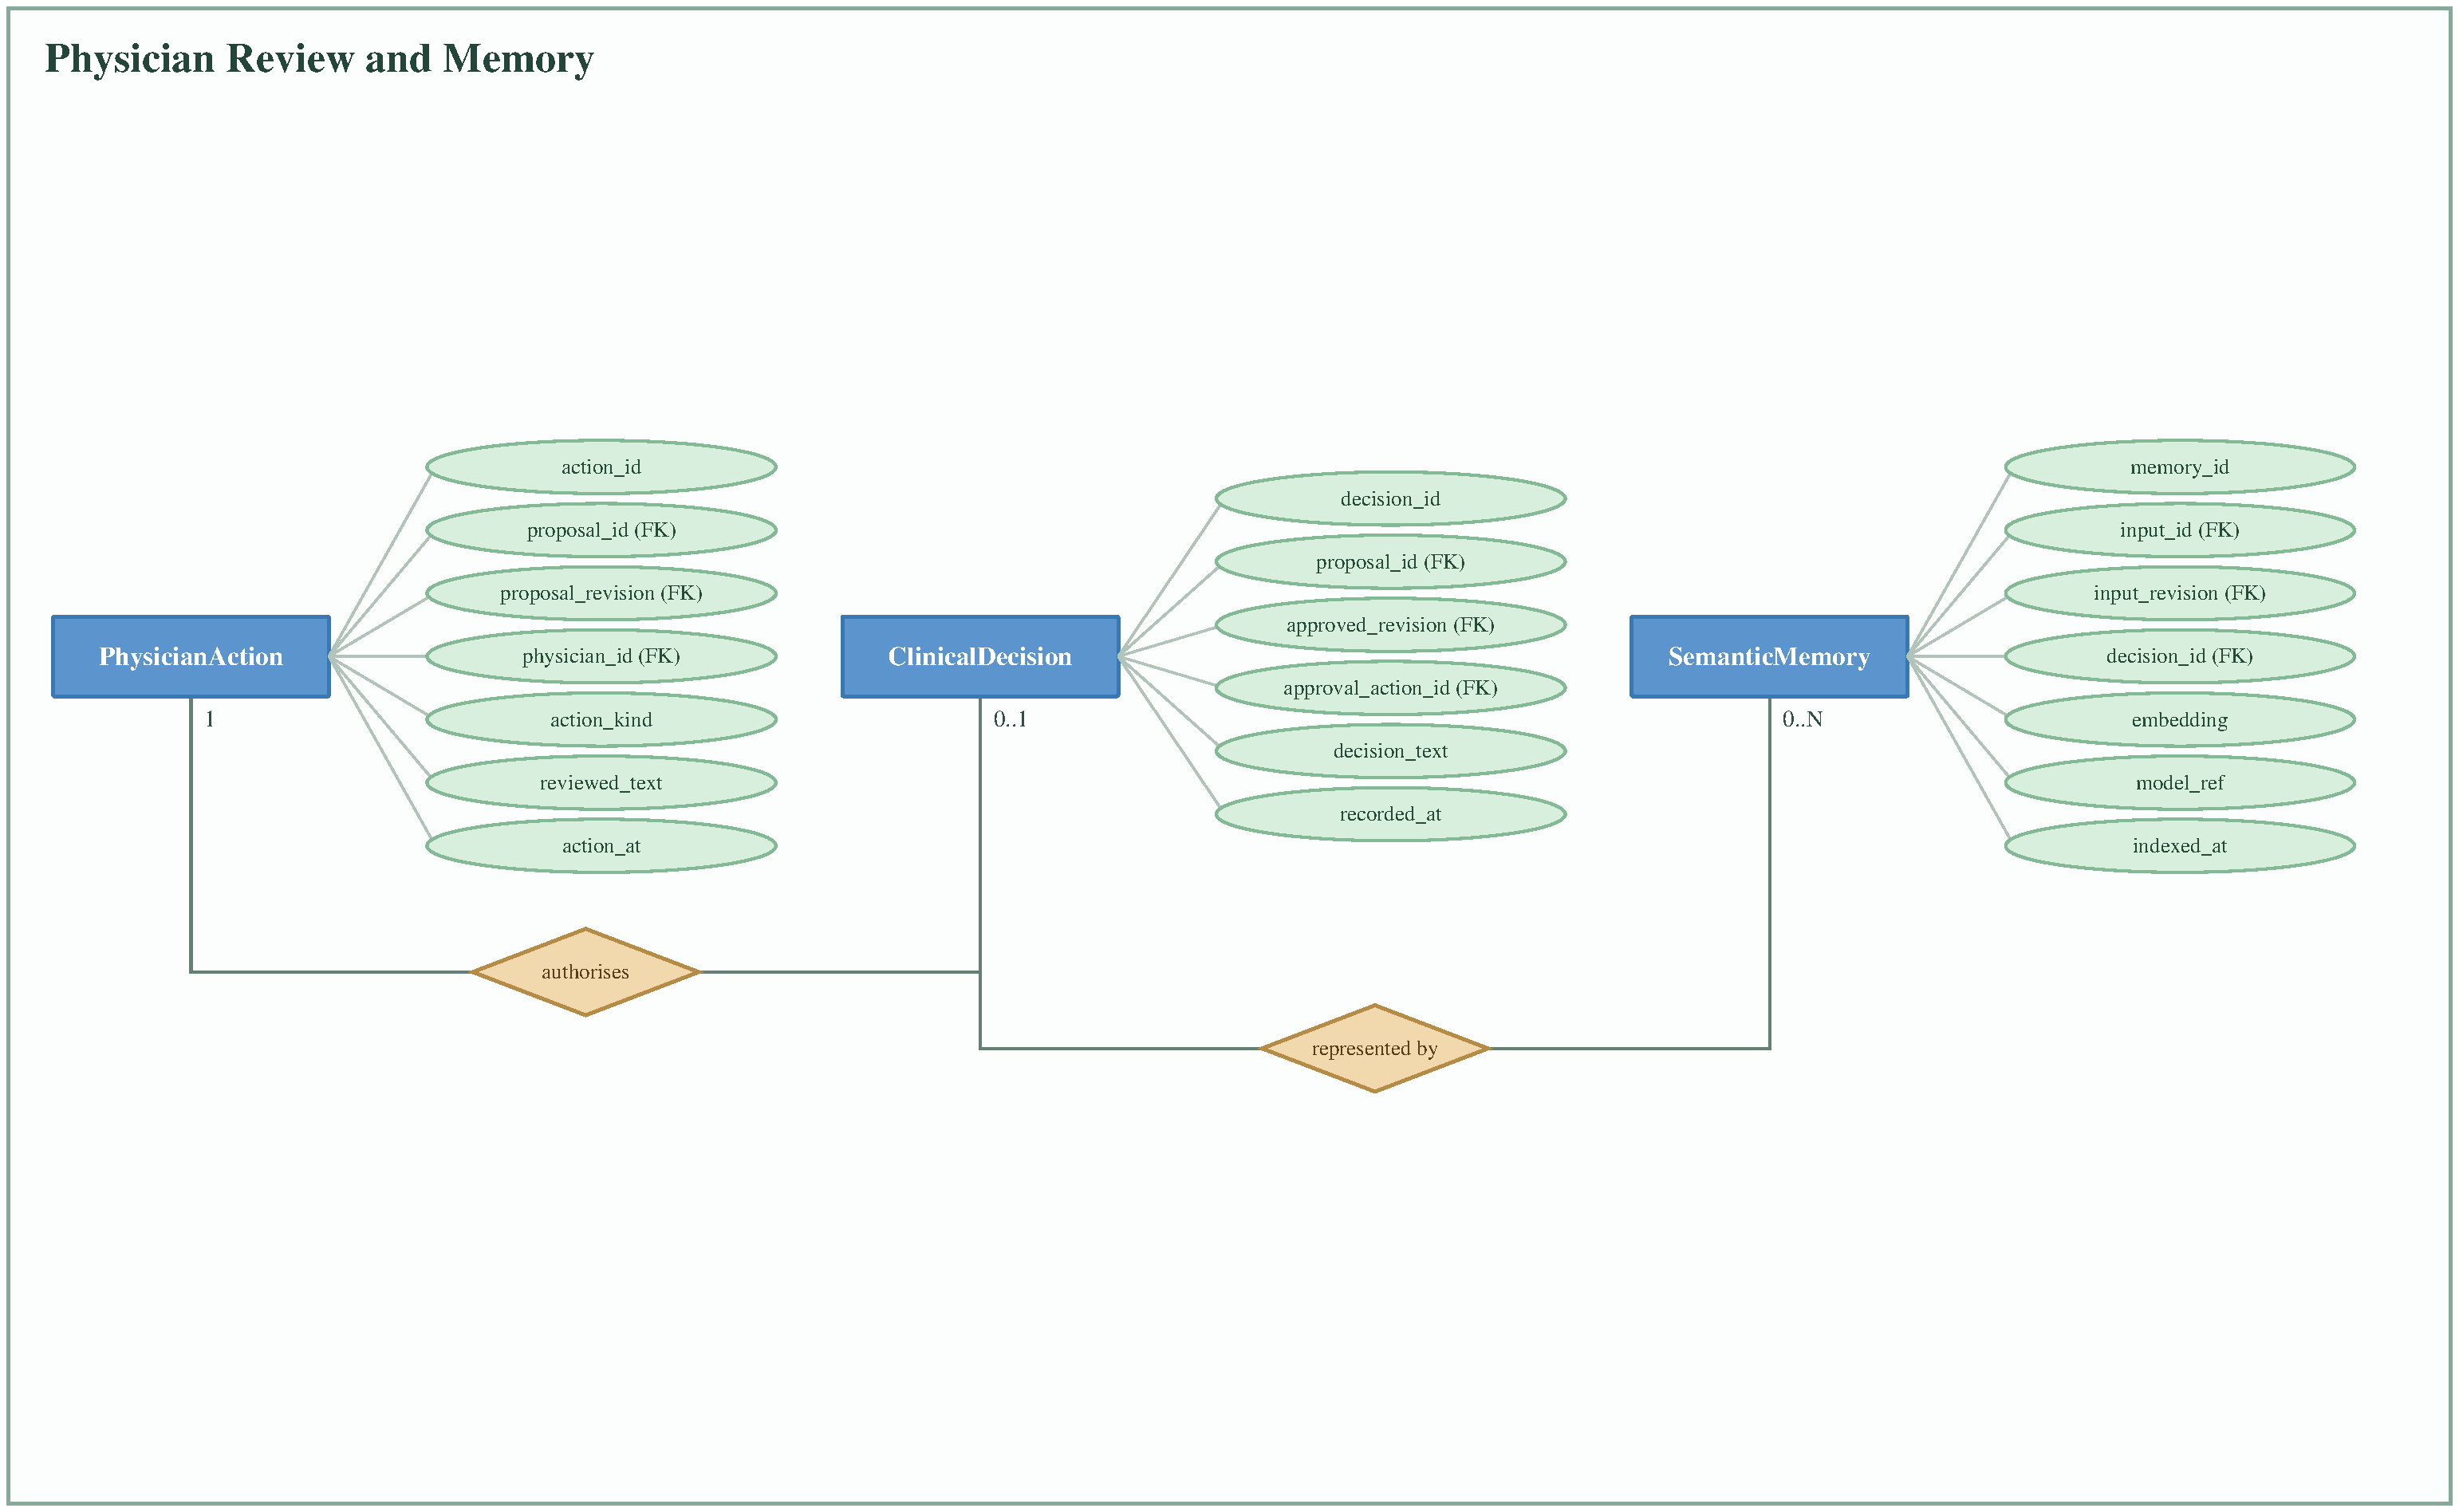
\includegraphics[width=\textwidth,height=0.80\textheight,keepaspectratio]{Figures/kashaf_D03_combined_review.pdf}
\caption{Physician actions, accepted decisions and semantic memory relationships.}
\label{fig:kashaf:er-review}
\end{figure}

\begin{figure}[!htbp]
\centering
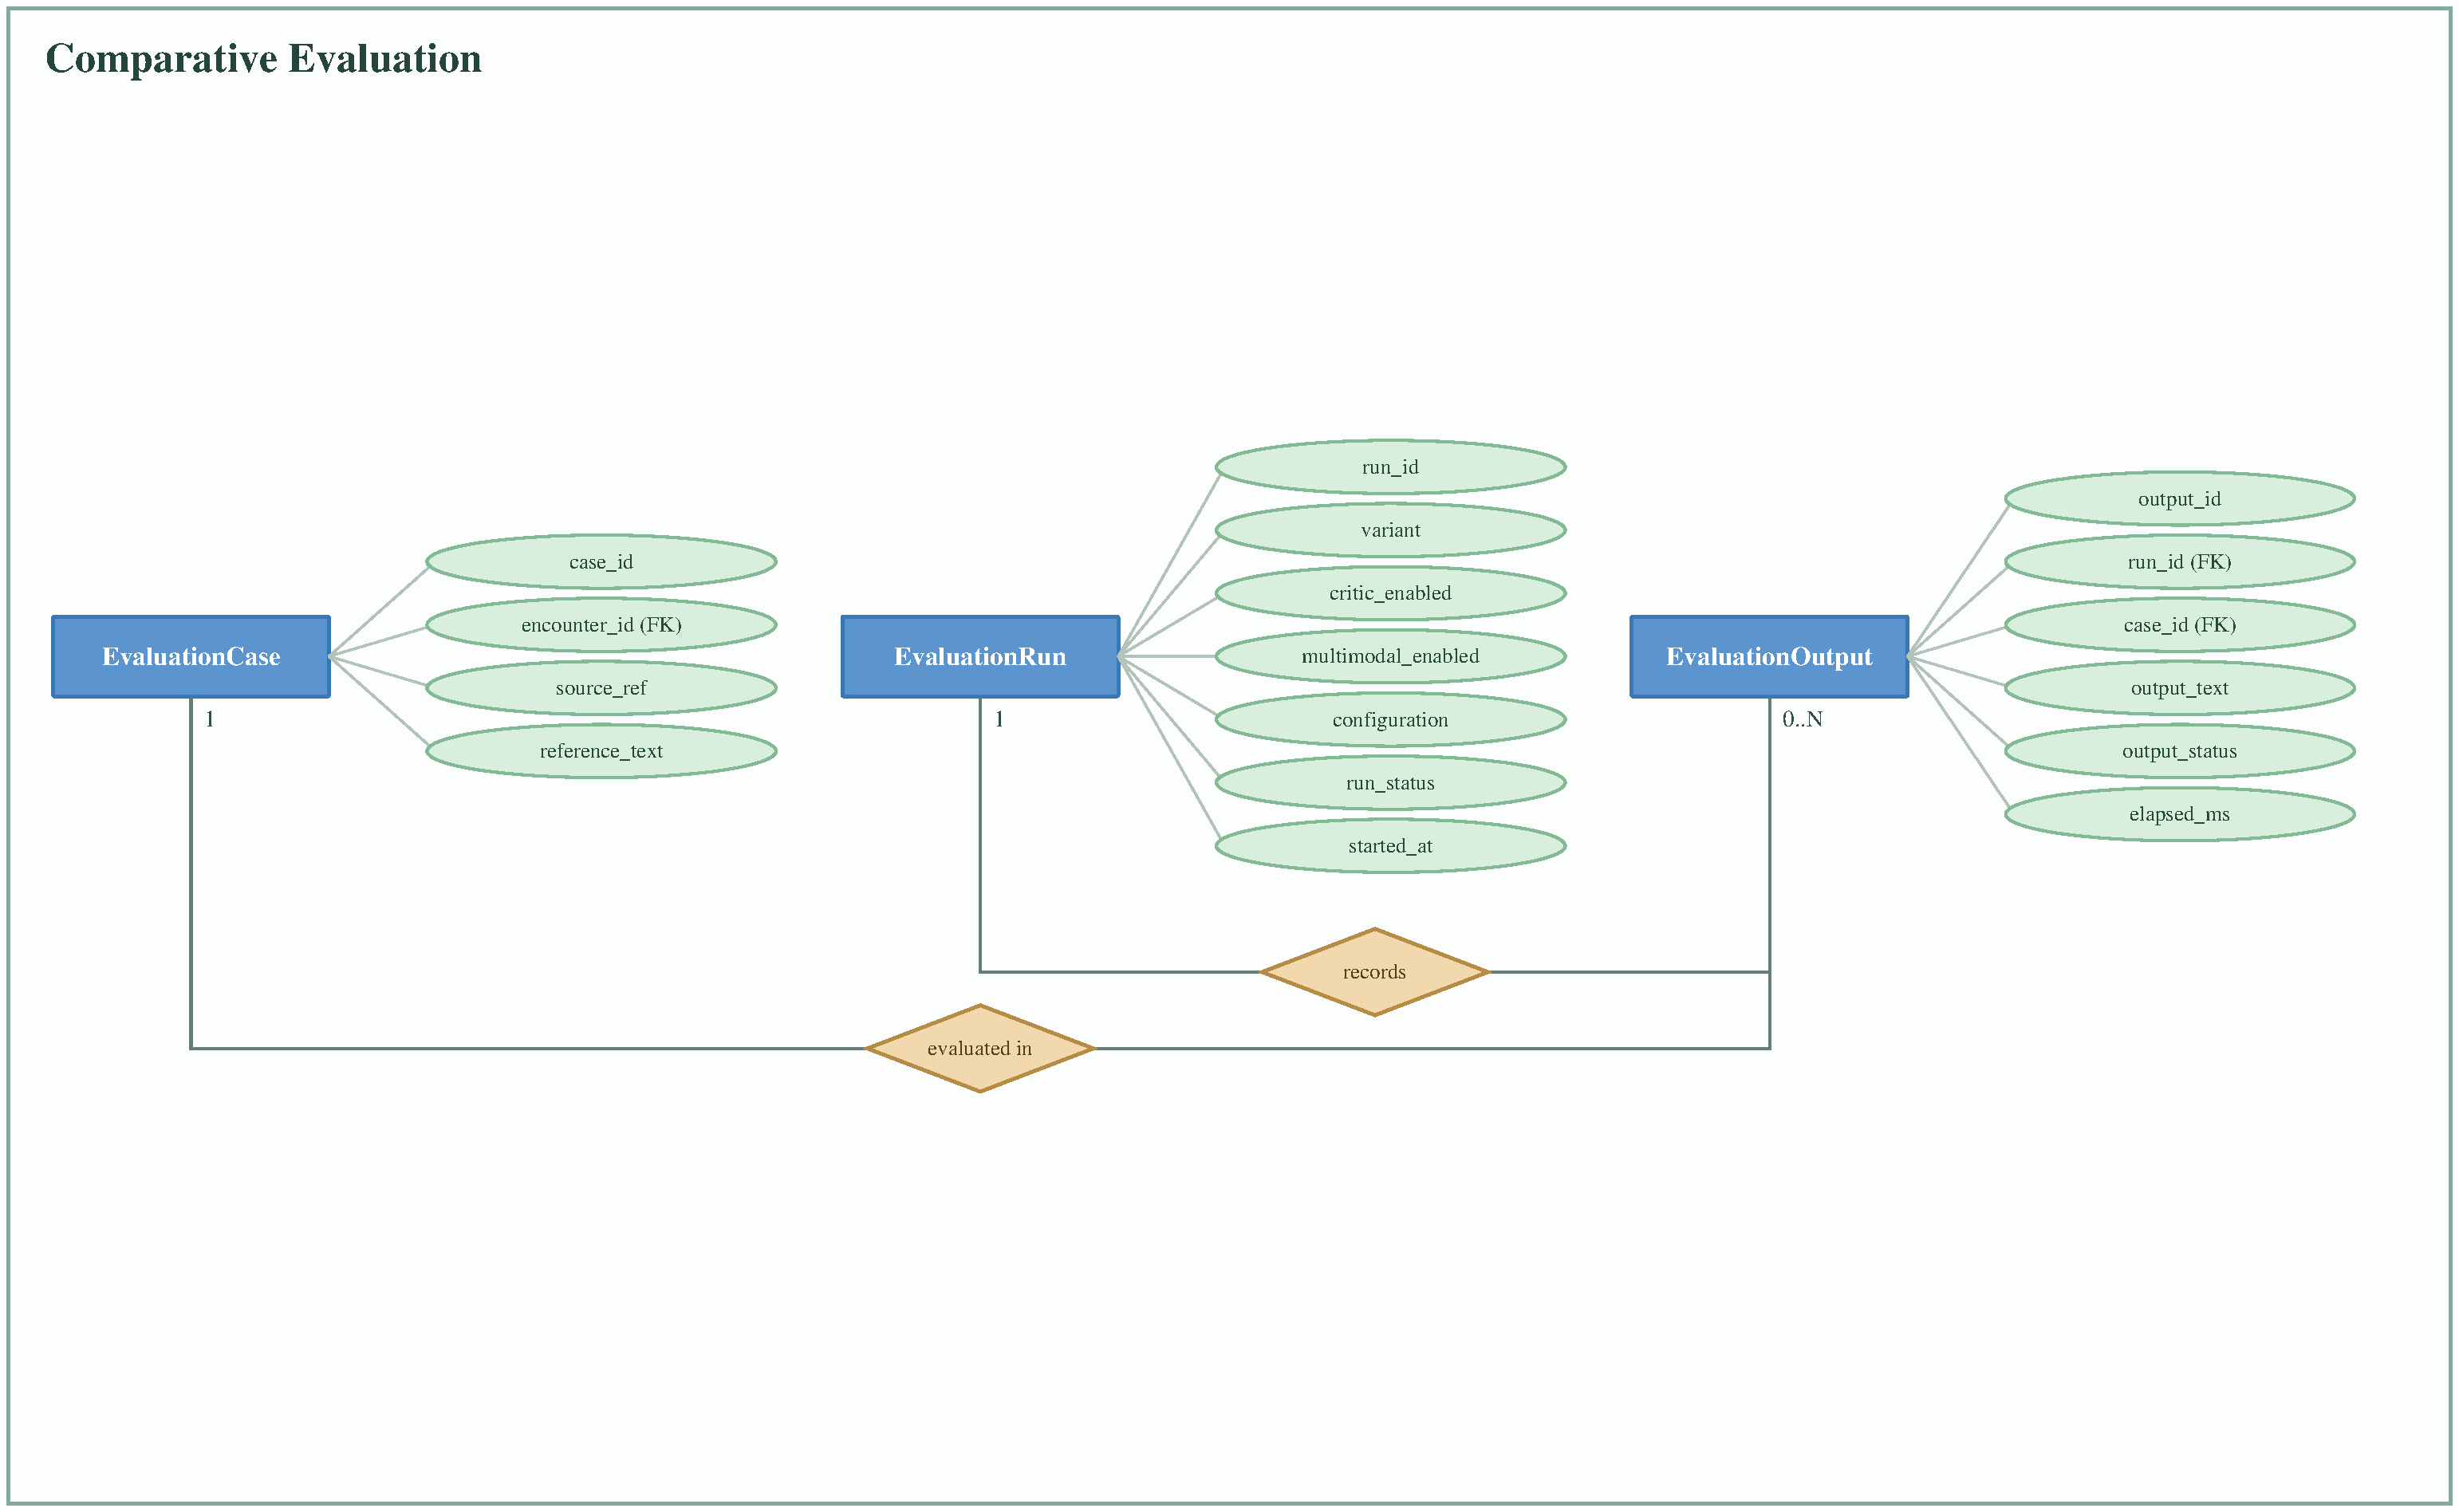
\includegraphics[width=\textwidth,height=0.80\textheight,keepaspectratio]{Figures/kashaf_D03_combined_evaluation.pdf}
\caption{Evaluation cases, configurations and recorded output relationships.}
\label{fig:kashaf:er-evaluation}
\end{figure}

\subsection{Data Dictionary}

Tables~\ref{tab:kashaf:dict-physician} onward define the entities, attributes, data types, constraints and meanings used by the logical schema. Primary keys identify records, composite keys preserve associations, and nullable fields accommodate absent values only where their processing state permits. Each patient's physician association governs access to encounters, case inputs, drafts, actions and decisions. Corrections create input revisions rather than replacing saved content; draft evidence, recorded critic findings and source links identify the exact revision they support. Approval validates the reviewed revision and physician action together, records matching accepted content, and permits at most one decision for that revision. Modified or rejected drafts remain outside accepted decisions. Semantic memory links authorised input revisions or approved decisions to their vector representations, with model-dependent dimensions configured after model selection. Evaluation fields describe case definitions, configurations and outputs; numerical measurements are populated only after an executed run. These relationships maintain source traceability without inventing missing clinical information.

\begin{reporttable}
\setlength{\tabcolsep}{5pt}
\centering
\small
\caption{Physician attributes, types and constraints.}
\label{tab:kashaf:dict-physician}
\begin{tabular}{|p{0.23\textwidth}|p{0.13\textwidth}|p{0.22\textwidth}|p{0.31\textwidth}|}
\hline
Attribute & Type & Constraints & Meaning \\ \hline
\texttt{physician\_id} & UUID & PK; not null & Unique physician account. \\ \hline
\texttt{full\_name} & text & Required; not null & Name supplied at registration. \\ \hline
\texttt{email} & text & Unique; not null & Normalised registration and login email. \\ \hline
\texttt{password\_hash} & text & Required; not null & Salted hash; plaintext passwords are never stored. \\ \hline
\texttt{created\_at} & timestamptz & Required; not null & Account creation time. \\ \hline
\end{tabular}
\end{reporttable}

\begin{reporttable}
\setlength{\tabcolsep}{5pt}
\centering
\small
\caption{Patient attributes, types and constraints.}
\label{tab:kashaf:dict-patient}
\begin{tabular}{|p{0.23\textwidth}|p{0.13\textwidth}|p{0.22\textwidth}|p{0.31\textwidth}|}
\hline
Attribute & Type & Constraints & Meaning \\ \hline
\texttt{patient\_id} & UUID & PK; not null & Unique patient record. \\ \hline
\texttt{physician\_id} & UUID & FK; not null & Physician who owns the record. \\ \hline
\texttt{patient\_ref} & text & Unique; not null & De-identified or synthetic reference. \\ \hline
\texttt{context\_text} & text & Optional; nullable & Available patient context. \\ \hline
\end{tabular}
\end{reporttable}

\begin{reporttable}
\setlength{\tabcolsep}{5pt}
\centering
\small
\caption{Encounter attributes, types and constraints.}
\label{tab:kashaf:dict-encounter}
\begin{tabular}{|p{0.23\textwidth}|p{0.13\textwidth}|p{0.22\textwidth}|p{0.31\textwidth}|}
\hline
Attribute & Type & Constraints & Meaning \\ \hline
\texttt{encounter\_id} & UUID & PK; not null & Unique encounter. \\ \hline
\texttt{patient\_id} & UUID & FK; not null & Patient associated with this encounter. \\ \hline
\texttt{recorded\_at} & timestamptz & Required; not null & Encounter date and time. \\ \hline
\end{tabular}
\end{reporttable}

\begin{reporttable}
\setlength{\tabcolsep}{5pt}
\centering
\small
\caption{ClinicalInput attributes, types and constraints.}
\label{tab:kashaf:dict-clinicalinput}
\begin{tabular}{|p{0.23\textwidth}|p{0.13\textwidth}|p{0.22\textwidth}|p{0.31\textwidth}|}
\hline
Attribute & Type & Constraints & Meaning \\ \hline
\texttt{input\_id} & UUID & PK; not null & Stable identifier of the supplied input. \\ \hline
\texttt{encounter\_id} & UUID & FK; not null & Encounter where the input originates. \\ \hline
\texttt{input\_kind} & text & Check; not null & Notes, imaging, laboratory or medication. \\ \hline
\end{tabular}
\end{reporttable}

\begin{reporttable}
\setlength{\tabcolsep}{5pt}
\centering
\small
\caption{InputRevision attributes, types and constraints.}
\label{tab:kashaf:dict-inputrevision}
\begin{tabular}{|p{0.23\textwidth}|p{0.13\textwidth}|p{0.22\textwidth}|p{0.31\textwidth}|}
\hline
Attribute & Type & Constraints & Meaning \\ \hline
\texttt{input\_id} & UUID & PK/FK; not null & Clinical input being versioned. \\ \hline
\texttt{revision\_no} & integer & PK; >0; not null & Saved revision of this input. \\ \hline
\texttt{content\_text} & text & Check; not null & Text content where applicable. \\ \hline
\texttt{file\_ref} & text & Check; not null & Stored file reference where applicable. \\ \hline
\texttt{recorded\_at} & timestamptz & Required; not null & Revision recording time. \\ \hline
\end{tabular}
\end{reporttable}

\begin{reporttable}
\setlength{\tabcolsep}{5pt}
\centering
\small
\caption{SpecialistFinding attributes, types and constraints.}
\label{tab:kashaf:dict-specialistfinding}
\begin{tabular}{|p{0.23\textwidth}|p{0.13\textwidth}|p{0.22\textwidth}|p{0.31\textwidth}|}
\hline
Attribute & Type & Constraints & Meaning \\ \hline
\texttt{finding\_id} & UUID & PK; not null & Unique analysis finding or processing record. \\ \hline
\texttt{input\_id} & UUID & FK pair; not null & Source clinical input. \\ \hline
\texttt{input\_revision} & integer & FK pair; not null & Exact analysed input revision. \\ \hline
\texttt{agent\_kind} & text & Check; not null & Imaging, laboratory or medication agent. \\ \hline
\texttt{model\_ref} & text & Optional; nullable & Model/resource identifier where applicable. \\ \hline
\texttt{finding\_text} & text & Check; not null & Available specialist findings. \\ \hline
\texttt{processing\_status} & text & Check; not null & Pending, complete or failed. \\ \hline
\texttt{processed\_at} & timestamptz & Optional; nullable & Completion or failure time. \\ \hline
\end{tabular}
\end{reporttable}

\begin{reporttable}
\setlength{\tabcolsep}{5pt}
\centering
\small
\caption{Proposal attributes, types and constraints.}
\label{tab:kashaf:dict-proposal}
\begin{tabular}{|p{0.23\textwidth}|p{0.13\textwidth}|p{0.22\textwidth}|p{0.31\textwidth}|}
\hline
Attribute & Type & Constraints & Meaning \\ \hline
\texttt{proposal\_id} & UUID & PK; not null & Stable identifier of a clinical draft. \\ \hline
\texttt{encounter\_id} & UUID & FK; not null & Encounter for which the draft is generated. \\ \hline
\texttt{created\_at} & timestamptz & Required; not null & Draft creation time. \\ \hline
\end{tabular}
\end{reporttable}

\begin{reporttable}
\setlength{\tabcolsep}{5pt}
\centering
\small
\caption{ProposalRevision attributes, types and constraints.}
\label{tab:kashaf:dict-proposalrevision}
\begin{tabular}{|p{0.23\textwidth}|p{0.13\textwidth}|p{0.22\textwidth}|p{0.31\textwidth}|}
\hline
Attribute & Type & Constraints & Meaning \\ \hline
\texttt{proposal\_id} & UUID & PK/FK; not null & Draft being versioned. \\ \hline
\texttt{revision\_no} & integer & PK; >0; not null & Saved draft revision. \\ \hline
\texttt{diagnosis\_text} & text & Required; not null & Generated or physician-edited diagnosis draft. \\ \hline
\texttt{treatment\_text} & text & Required; not null & Generated or physician-edited treatment draft. \\ \hline
\texttt{review\_status} & text & Check; not null & Pending, approved or rejected. \\ \hline
\texttt{created\_at} & timestamptz & Required; not null & Time this revision is saved. \\ \hline
\end{tabular}
\end{reporttable}

\begin{reporttable}
\setlength{\tabcolsep}{5pt}
\centering
\small
\caption{ProposalInput attributes, types and constraints.}
\label{tab:kashaf:dict-proposalinput}
\begin{tabular}{|p{0.23\textwidth}|p{0.13\textwidth}|p{0.22\textwidth}|p{0.31\textwidth}|}
\hline
Attribute & Type & Constraints & Meaning \\ \hline
\texttt{proposal\_id} & UUID & PK/FK pair; not null & Draft using the input. \\ \hline
\texttt{proposal\_revision} & integer & PK/FK pair; not null & Exact draft revision. \\ \hline
\texttt{input\_id} & UUID & PK/FK pair; not null & Current or historical source input. \\ \hline
\texttt{input\_revision} & integer & PK/FK pair; not null & Exact source input revision used. \\ \hline
\end{tabular}
\end{reporttable}

\begin{reporttable}
\setlength{\tabcolsep}{5pt}
\centering
\small
\caption{CriticReview attributes, types and constraints.}
\label{tab:kashaf:dict-criticreview}
\begin{tabular}{|p{0.23\textwidth}|p{0.13\textwidth}|p{0.22\textwidth}|p{0.31\textwidth}|}
\hline
Attribute & Type & Constraints & Meaning \\ \hline
\texttt{critic\_id} & UUID & PK; not null & Unique critic-review operation. \\ \hline
\texttt{proposal\_id} & UUID & FK pair; not null & Assessed clinical draft. \\ \hline
\texttt{proposal\_revision} & integer & FK pair; not null & Exact assessed revision. \\ \hline
\texttt{review\_status} & text & Check; not null & Pending, complete or failed. \\ \hline
\texttt{findings\_text} & text & Check; not null & Safety and consistency findings when complete. \\ \hline
\texttt{reviewed\_at} & timestamptz & Optional; nullable & Time the review completes or fails. \\ \hline
\end{tabular}
\end{reporttable}

\begin{reporttable}
\setlength{\tabcolsep}{5pt}
\centering
\small
\caption{EvidenceItem attributes, types and constraints.}
\label{tab:kashaf:dict-evidenceitem}
\begin{tabular}{|p{0.23\textwidth}|p{0.13\textwidth}|p{0.22\textwidth}|p{0.31\textwidth}|}
\hline
Attribute & Type & Constraints & Meaning \\ \hline
\texttt{evidence\_id} & UUID & PK; not null & Unique retrieved evidence item. \\ \hline
\texttt{source\_ref} & text & Required; not null & Citation or source reference. \\ \hline
\texttt{passage\_text} & text & Required; not null & Retrieved supporting passage. \\ \hline
\texttt{retrieved\_at} & timestamptz & Required; not null & Evidence retrieval time. \\ \hline
\end{tabular}
\end{reporttable}

\begin{reporttable}
\setlength{\tabcolsep}{5pt}
\centering
\small
\caption{ProposalEvidence attributes, types and constraints.}
\label{tab:kashaf:dict-proposalevidence}
\begin{tabular}{|p{0.23\textwidth}|p{0.13\textwidth}|p{0.22\textwidth}|p{0.31\textwidth}|}
\hline
Attribute & Type & Constraints & Meaning \\ \hline
\texttt{proposal\_id} & UUID & PK/FK pair; not null & Draft supported by evidence. \\ \hline
\texttt{proposal\_revision} & integer & PK/FK pair; not null & Exact supported revision. \\ \hline
\texttt{evidence\_id} & UUID & PK/FK; not null & Retrieved evidence item. \\ \hline
\end{tabular}
\end{reporttable}

\begin{reporttable}
\setlength{\tabcolsep}{5pt}
\centering
\small
\caption{PhysicianAction attributes, types and constraints.}
\label{tab:kashaf:dict-physicianaction}
\begin{tabular}{|p{0.23\textwidth}|p{0.13\textwidth}|p{0.22\textwidth}|p{0.31\textwidth}|}
\hline
Attribute & Type & Constraints & Meaning \\ \hline
\texttt{action\_id} & UUID & PK; not null & Unique physician review action. \\ \hline
\texttt{proposal\_id} & UUID & FK pair; not null & Clinical draft being reviewed. \\ \hline
\texttt{proposal\_revision} & integer & FK pair; not null & Exact reviewed revision. \\ \hline
\texttt{physician\_id} & UUID & FK; not null & Physician performing the action. \\ \hline
\texttt{action\_kind} & text & Check; not null & Modify, approve or reject. \\ \hline
\texttt{reviewed\_text} & text & Required; not null & Snapshot of the content associated with the action. \\ \hline
\texttt{action\_at} & timestamptz & Required; not null & Action recording time. \\ \hline
\end{tabular}
\end{reporttable}

\begin{reporttable}
\setlength{\tabcolsep}{5pt}
\centering
\small
\caption{ClinicalDecision attributes, types and constraints.}
\label{tab:kashaf:dict-clinicaldecision}
\begin{tabular}{|p{0.23\textwidth}|p{0.13\textwidth}|p{0.22\textwidth}|p{0.31\textwidth}|}
\hline
Attribute & Type & Constraints & Meaning \\ \hline
\texttt{decision\_id} & UUID & PK; not null & Unique approved clinical decision. \\ \hline
\texttt{proposal\_id} & UUID & FK pair; not null & Originating clinical draft. \\ \hline
\texttt{approved\_revision} & integer & FK pair; unique pair; not null & Explicitly accepted draft revision. \\ \hline
\texttt{approval\_action\_id} & UUID & Unique FK; not null & Matching physician approval action. \\ \hline
\texttt{decision\_text} & text & Required; not null & Exact accepted diagnosis and treatment content. \\ \hline
\texttt{recorded\_at} & timestamptz & Required; not null & Decision recording time. \\ \hline
\end{tabular}
\end{reporttable}

\begin{reporttable}
\setlength{\tabcolsep}{5pt}
\centering
\small
\caption{SemanticMemory attributes, types and constraints.}
\label{tab:kashaf:dict-semanticmemory}
\begin{tabular}{|p{0.23\textwidth}|p{0.13\textwidth}|p{0.22\textwidth}|p{0.31\textwidth}|}
\hline
Attribute & Type & Constraints & Meaning \\ \hline
\texttt{memory\_id} & UUID & PK; not null & Unique semantic representation. \\ \hline
\texttt{input\_id} & UUID & FK pair; not null & Input source when applicable. \\ \hline
\texttt{input\_revision} & integer & FK pair; not null & Exact input-source revision. \\ \hline
\texttt{decision\_id} & UUID & FK; not null & Approved-decision source when applicable. \\ \hline
\texttt{embedding} & vector(TBD) & Required; not null & Vector using the selected embedding dimension. \\ \hline
\texttt{model\_ref} & text & Required; not null & Embedding model identifier and version. \\ \hline
\texttt{indexed\_at} & timestamptz & Required; not null & Indexing time. \\ \hline
\end{tabular}
\end{reporttable}

\begin{reporttable}
\setlength{\tabcolsep}{5pt}
\centering
\small
\caption{EvaluationCase attributes, types and constraints.}
\label{tab:kashaf:dict-evaluationcase}
\begin{tabular}{|p{0.23\textwidth}|p{0.13\textwidth}|p{0.22\textwidth}|p{0.31\textwidth}|}
\hline
Attribute & Type & Constraints & Meaning \\ \hline
\texttt{case\_id} & UUID & PK; not null & Unique permitted evaluation case. \\ \hline
\texttt{encounter\_id} & UUID & FK; not null & Case encounter supplying clinical context. \\ \hline
\texttt{source\_ref} & text & Required; not null & Dataset or synthetic-case provenance. \\ \hline
\texttt{reference\_text} & text & Optional; nullable & Reference assessment when established. \\ \hline
\end{tabular}
\end{reporttable}

\begin{reporttable}
\setlength{\tabcolsep}{5pt}
\centering
\small
\caption{EvaluationRun attributes, types and constraints.}
\label{tab:kashaf:dict-evaluationrun}
\begin{tabular}{|p{0.23\textwidth}|p{0.13\textwidth}|p{0.22\textwidth}|p{0.31\textwidth}|}
\hline
Attribute & Type & Constraints & Meaning \\ \hline
\texttt{run\_id} & UUID & PK; not null & Unique configured research run. \\ \hline
\texttt{variant} & text & Check; not null & Single LLM, memory-augmented or full Zeest. \\ \hline
\texttt{critic\_enabled} & boolean & Required; not null & Declared critic configuration. \\ \hline
\texttt{multimodal\_enabled} & boolean & Required; not null & Declared multimodal configuration. \\ \hline
\texttt{configuration} & jsonb & Required; not null & Model/resource versions and comparison settings. \\ \hline
\texttt{run\_status} & text & Check; not null & Configured, running, complete or failed. \\ \hline
\texttt{started\_at} & timestamptz & Optional; nullable & Actual run start time, when executed. \\ \hline
\end{tabular}
\end{reporttable}

\begin{reporttable}
\setlength{\tabcolsep}{5pt}
\centering
\small
\caption{EvaluationOutput attributes, types and constraints.}
\label{tab:kashaf:dict-evaluationoutput}
\begin{tabular}{|p{0.23\textwidth}|p{0.13\textwidth}|p{0.22\textwidth}|p{0.31\textwidth}|}
\hline
Attribute & Type & Constraints & Meaning \\ \hline
\texttt{output\_id} & UUID & PK; not null & Unique run/case output. \\ \hline
\texttt{run\_id} & UUID & FK; unique pair; not null & Research run producing this output. \\ \hline
\texttt{case\_id} & UUID & FK; unique pair; not null & Evaluation case used by the run. \\ \hline
\texttt{output\_text} & text & Check; not null & Recorded system output after execution. \\ \hline
\texttt{output\_status} & text & Check; not null & Pending, complete or failed. \\ \hline
\texttt{elapsed\_ms} & numeric & Optional; >=0; nullable & Measured duration only when available. \\ \hline
\end{tabular}
\end{reporttable}


\section{ Risk Analysis}

\begin{reporttable}
\centering
\small
\caption{Project risks, consequences and intended responses.}
\label{tab:kashaf:risks}
\begin{tabular}{|p{0.06\textwidth}|p{0.2\textwidth}|p{0.27\textwidth}|p{0.33\textwidth}|}
\hline
ID & Risk & Consequence & Response \\ \hline
R01 & Data/model access & The selected clinical domain cannot be supported. & Confirm permitted cases and validated models before integration. \\ \hline
R02 & Transcription/input quality & Incomplete or incorrect case information. & Allow note correction and report unusable inputs. \\ \hline
R03 & Insufficient evidence & Draft recommendations lack inspectable support. & Show retrieved sources and make missing evidence explicit. \\ \hline
R04 & Unsupported reasoning & Recommendations contain inconsistent findings. & Use critic review and retain physician decision authority. \\ \hline
R05 & Patient-context mismatch & History or inputs are assigned to the wrong case. & Validate patient/encounter keys across processing and storage. \\ \hline
R06 & Approval/revision error & Recorded content differs from the physician-approved draft. & Bind approval to the exact revision and content snapshot. \\ \hline
R07 & Integration/service failure & The processing workflow is incomplete or incompatible. & Define contracts and expose stage-specific failures. \\ \hline
R08 & Evaluation resources & Variant comparisons cannot answer the research questions. & Agree references, common cases and comparison conditions. \\ \hline
\end{tabular}
\end{reporttable}

% Finish this section's floats before the next heading.

Table~\ref{tab:kashaf:risks} outlines risks concerning resource permissions, supported clinical coverage, incomplete evidence, incorrect patient context and revision-specific approval. Their responses establish verification activities rather than completed mitigation outcomes. Dataset and model selection must confirm permitted use and task suitability before cases enter processing or comparison. Source identifiers and ownership checks must remain consistent through retrieval, analysis and review, while unavailable resources require visible failure states. Evidence inspection and critic findings support physician judgement without guaranteeing correctness. Approval must accept the reviewed revision and preserve matching action and decision records, including when requests fail or repeat. Integration tests and controlled comparisons are needed to assess these responses after implementation. The requirements, use cases, interface designs and logical schema therefore define a clinical workflow, while the methodology and architecture specify how its behaviour can be investigated. No performance result, executed acceptance test or demonstrated clinical safety outcome is established by these design artefacts.

\section{Conclusion}

The requirements establish a connected workflow from account access and physician-specific patient selection to consultation capture, specialist findings and clinical review. Functional requirements identify the operations users need, while quality attributes and non-functional requirements define ownership, integrity, traceability and understandable processing states. Use-case tables describe normal and alternative paths, and interface mappings connect these interactions to the corresponding screens. The logical schema preserves input revisions, draft sources, review actions and accepted decisions so corrections and approval refer to identifiable content. Registration supports account access without introducing additional clinical roles, and each physician remains restricted to their own patients. Together, these specifications make the intended behaviour assessable through functional and integrity checks. Numerical performance limits and clinical resource configurations require an agreed environment before measurement. The requirements provide the contract for implementation and evaluation; they do not establish completed acceptance tests or clinical effectiveness. Subsequent design must preserve these relationships when connecting application services, agents and storage.

\endgroup
%
% Owner: Fatima Malik / Member B.
% Local font encoding restores the template's Times regular/bold faces under XeTeX.
\begingroup
\renewcommand{\encodingdefault}{T1}
\fontencoding{T1}\selectfont
\chapter{Proposed Approach and Methodology}
Zeest uses an integration methodology rather than a new diagnostic algorithm. The method begins with a physician-selected patient and encounter, then prepares consultation notes, clinical inputs and relevant longitudinal history. Existing imaging models, clinical language-model capability and retrieval methods act as supporting components, while the project contribution is the way their outputs connect to patient memory, evidence and physician approval. Chapter~4 defines the workflow for navigation, transcription, input handling, memory retrieval, draft generation, critic review and revision-specific decisions. This chapter turns those requirements into a controlled research procedure in which each stage keeps patient, encounter and source context visible, so a generated draft can be inspected rather than treated as final. The methodology is organised around three questions: how the current encounter and history should be prepared for specialised agents, how external evidence should be retrieved and attached to the draft for physician review, and how variants should be compared so memory, agent decomposition, critic review and multimodal inputs can be assessed. The answers are expressed as a processing pipeline, dataset and model register, evidence-retrieval procedure and ablation protocol.

\section{Case Preparation and Input Handling}
The first methodological step is to create a consistent case package for the selected encounter. The physician opens a patient record, reviews prior encounters and begins or uploads consultation information according to the workflow defined in Chapter~4. Consultation audio is prepared as structured notes, which the physician can inspect and correct before downstream use. Imaging, laboratory information and medication context remain separate because they have different representations, source formats and analysis needs. Each input must retain its patient identifier, encounter identifier, type, source reference and revision. This prevents later stages from mixing old notes with the current encounter or treating unsupported input as a finding. The prepared package therefore describes what information is available, where it came from and whether it is ready for analysis. This also keeps failed or missing inputs visible instead of hiding them inside the draft generation process. The purpose of this stage is not to diagnose the patient, but to create a clear and traceable input state for memory retrieval, specialist analysis and later comparison.

\section{Hybrid Memory and Case Organisation}
Hybrid memory connects the current encounter to relevant historical context. Relational records preserve patient, encounter, input and approved-decision relationships, while semantic retrieval selects history related to the current consultation or clinical question. The Patient Memory Agent returns source-aware context, not a final diagnosis. The Clinical Case Agent then organises corrected notes, retrieved history and specialist inputs into a case representation for later reasoning. This package identifies what is current, what is historical, what was retrieved and what is missing. If an input is absent or fails validation, that status is carried forward instead of creating a placeholder finding. This approach aligns with the database design in Chapter~4, where clinical inputs, drafts, evidence, audit actions and approved decisions are separate records. It also supports the planned comparison with a single-LLM baseline, because the baseline receives less patient-specific structure than the memory and full-system variants. The case organisation stage is therefore the bridge between raw encounter information and the controlled agent workflow.

\section{Proposed Agent Processing Pipeline}
Figure~\ref{fig:fatima:method-pipeline} shows the processing pipeline used to coordinate the proposed Zeest workflow. The physician-facing interface produces current case inputs, while hybrid memory supplies patient history. The Clinical Case Agent combines those inputs and sends modality-specific information to the Imaging, Laboratory and Medication Safety agents. The Imaging Agent uses an existing validated pre-trained model only for supported imaging tasks. The Laboratory Agent analyses supplied laboratory information, and the Medication Safety Agent checks medication context against a resource still to be selected. The Evidence and RAG Agent retrieves external clinical material with source references. The Clinical Reasoning Agent drafts the diagnosis and treatment proposal, and the Safety and Critic Agent checks it before physician review. The pipeline separates data movement from decision authority. Agents may prepare, analyse, retrieve or review information, but they do not record a final clinical decision. The physician sees the draft with evidence and critic findings, then approves, modifies or rejects it. Approval records the accepted revision, modification creates a changed draft, and rejection keeps the draft out of approved decisions.

\begin{figure}[htbp]
\centering
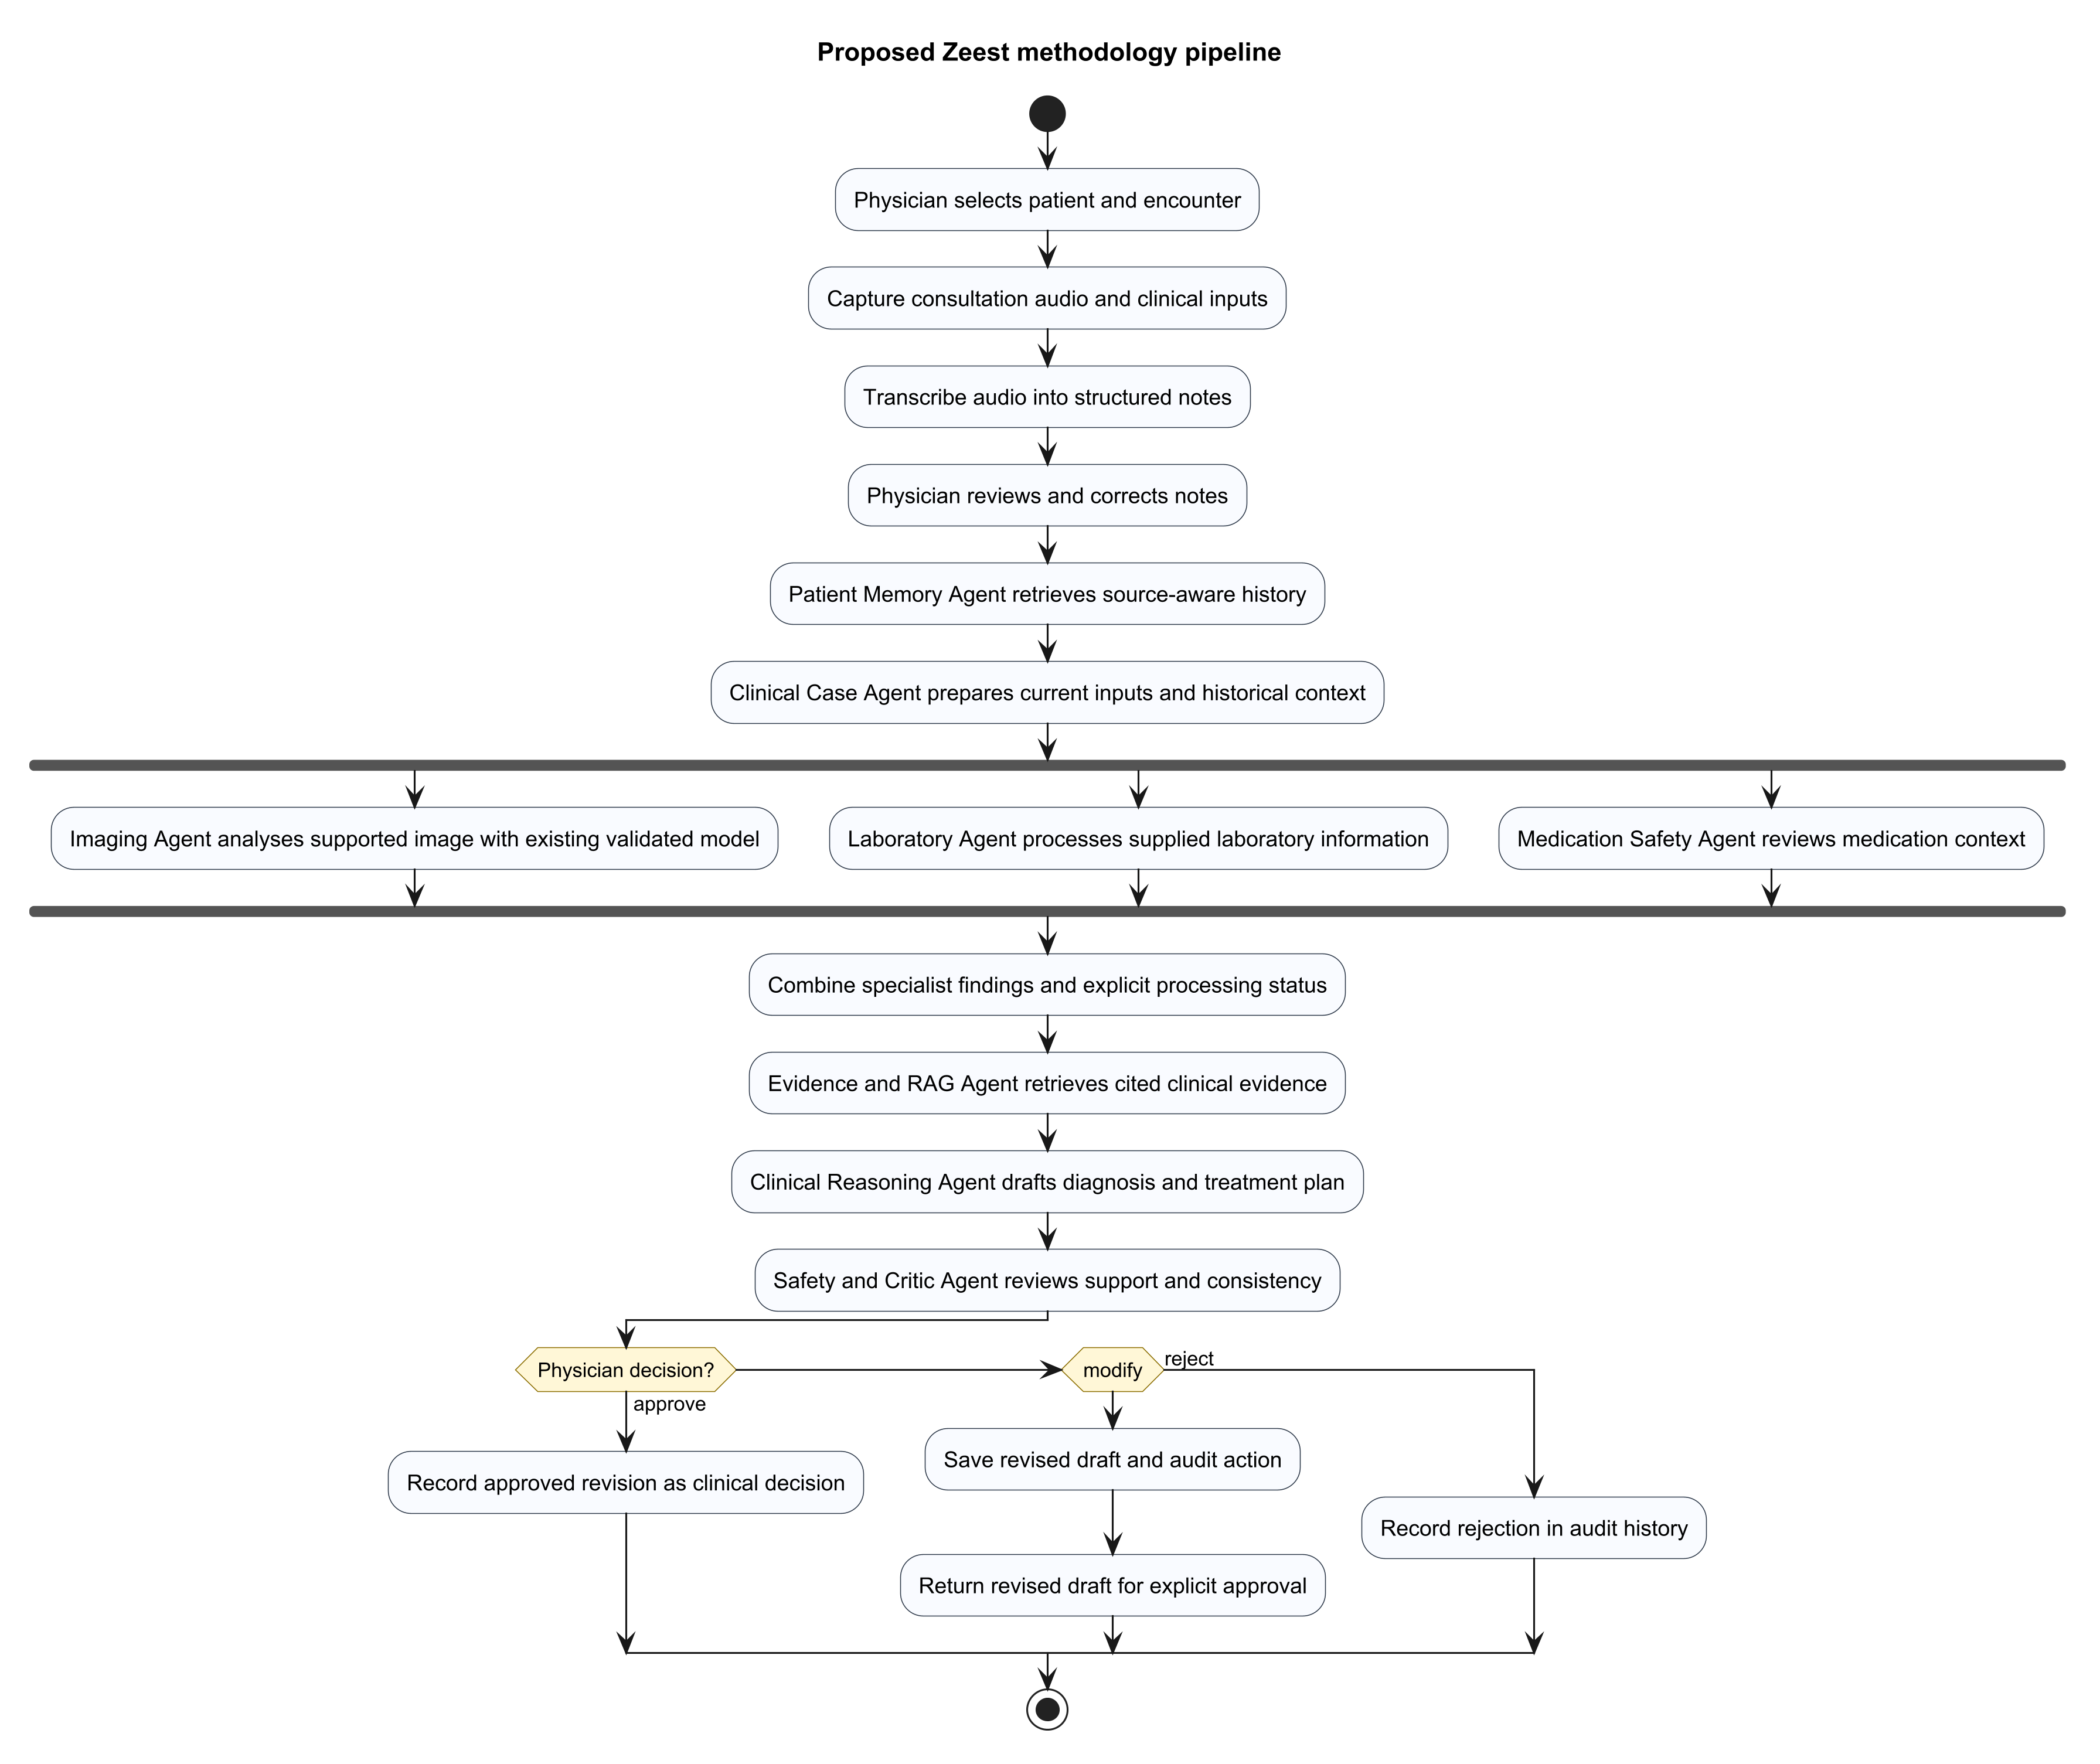
\includegraphics[width=0.96\textwidth,height=0.78\textheight,keepaspectratio]{Figures/fatima_D04_method_pipeline.png}
\caption{Proposed Zeest methodology pipeline connecting consultation inputs, hybrid memory, specialist agents, evidence retrieval, clinical drafting, critic review and physician decision controls.}
\label{fig:fatima:method-pipeline}
\end{figure}

\section{Dataset, Model and Resource Register}
The candidate data and model resources come from the proposal and literature review. MIMIC-IV supports de-identified longitudinal EHR cases, while MIMIC-CXR and CheXpert support chest radiograph tasks. PubMed or guideline sources may support evidence retrieval, and Synthea can support synthetic patient cases.\cite{zeestA:mimicIV,zeestB:mimiccxr,zeestB:chexpert,zeestB:synthea} These resources are not interchangeable. Longitudinal memory needs encounter context, while imaging cases must match the selected model's supported labels. Evidence retrieval needs a permitted corpus and citation preservation. Medication review requires a knowledge resource with suitable coverage, and semantic memory requires an embedding model compatible with the vector store. Table~\ref{tab:fatima:dataset-register} records each candidate's role, status and unresolved dependency so final selection is not assumed before implementation. This register keeps the methodology honest: a proposal-listed resource becomes usable only after access, permitted use, preprocessing needs and clinical-domain fit are confirmed. It also gives later evaluation work a checklist for deciding which cases and modalities can be included in the ablation study.

\begin{table}[htbp]
\centering
\scriptsize
\caption{Proposed dataset, model and resource register for Zeest methodology.}
\label{tab:fatima:dataset-register}
\begin{tabular}{|p{0.19\textwidth}|p{0.24\textwidth}|p{0.21\textwidth}|p{0.22\textwidth}|}
\hline
Candidate & Planned role & Current status & Dependency \\ \hline
MIMIC-IV \cite{zeestA:mimicIV} & Longitudinal EHR-style case context. & Candidate source. & Access, permitted use and case selection. \\ \hline
MIMIC-CXR \cite{zeestB:mimiccxr} & Chest radiograph and report context. & Candidate source. & Access, pairing and supported task. \\ \hline
CheXpert \cite{zeestB:chexpert} & Imaging benchmark/model candidate domain. & Candidate source. & Final model and label compatibility. \\ \hline
Existing imaging classifier & Supported imaging finding generation. & Not selected. & Validated model, inputs and labels. \\ \hline
PubMed/guideline corpus & External evidence retrieval. & Not finalised. & Corpus choice, citation format and retrieval policy. \\ \hline
Synthea \cite{zeestB:synthea} & Synthetic workflow cases. & Candidate source. & Scenario realism and mapping to Zeest fields. \\ \hline
Medication knowledge resource & Medication safety checking. & Not selected. & Resource availability and interaction coverage. \\ \hline
Embedding model & Semantic memory and retrieval. & Not selected. & Dimension, domain suitability and pgvector storage. \\ \hline
\end{tabular}
\end{table}

\section{Data Preprocessing}
Preprocessing depends on the chosen resources, but Zeest's workflow already defines the preparation rules. Patient and encounter identifiers must be de-identified or synthetic. Consultation notes, reports and other text inputs should be structured while remaining linked to their source. Imaging files should follow only the selected model's required input format, because changing image preparation without matching the model can invalidate the finding. Laboratory and medication information should be normalised enough for the relevant agent to interpret it, but missing values should not be invented. Evidence passages should retain source references and retrieval timestamps. Ablation cases should be frozen before comparison so each variant receives the same allowed inputs for its configuration. This prevents a memory-augmented variant or full-system variant from benefiting from accidental case changes. The preprocessing stage therefore supports both system correctness and evaluation fairness. It prepares the data for analysis while preserving the traceability needed for physician review, critic checking and later reporting.

\section{Evidence Retrieval Method}
The evidence method separates patient-specific context from external clinical knowledge. Patient context comes from the selected encounter, corrected notes, retrieved history and specialist findings. External knowledge comes from guideline, literature or medical reference material selected for retrieval. The Evidence and RAG Agent forms a query from the case context, retrieves candidate passages, filters or ranks them by relevance and returns supporting text with citations. Figure~\ref{fig:fatima:evidence-retrieval} shows this flow. The Clinical Reasoning Agent may use retrieved evidence when drafting a diagnosis and treatment plan, but the evidence must remain visible to the physician. This prevents a black box answer and lets the critic identify unsupported claims, missing evidence or contradictions. The procedure also supports traceability because a draft should identify which retrieved passages were used and where they came from. The physician can then judge whether the support fits the current patient and whether the draft should be approved, edited or rejected. If evidence is insufficient, the interface should show that status instead of fabricating support.

\begin{figure}[htbp]
\centering
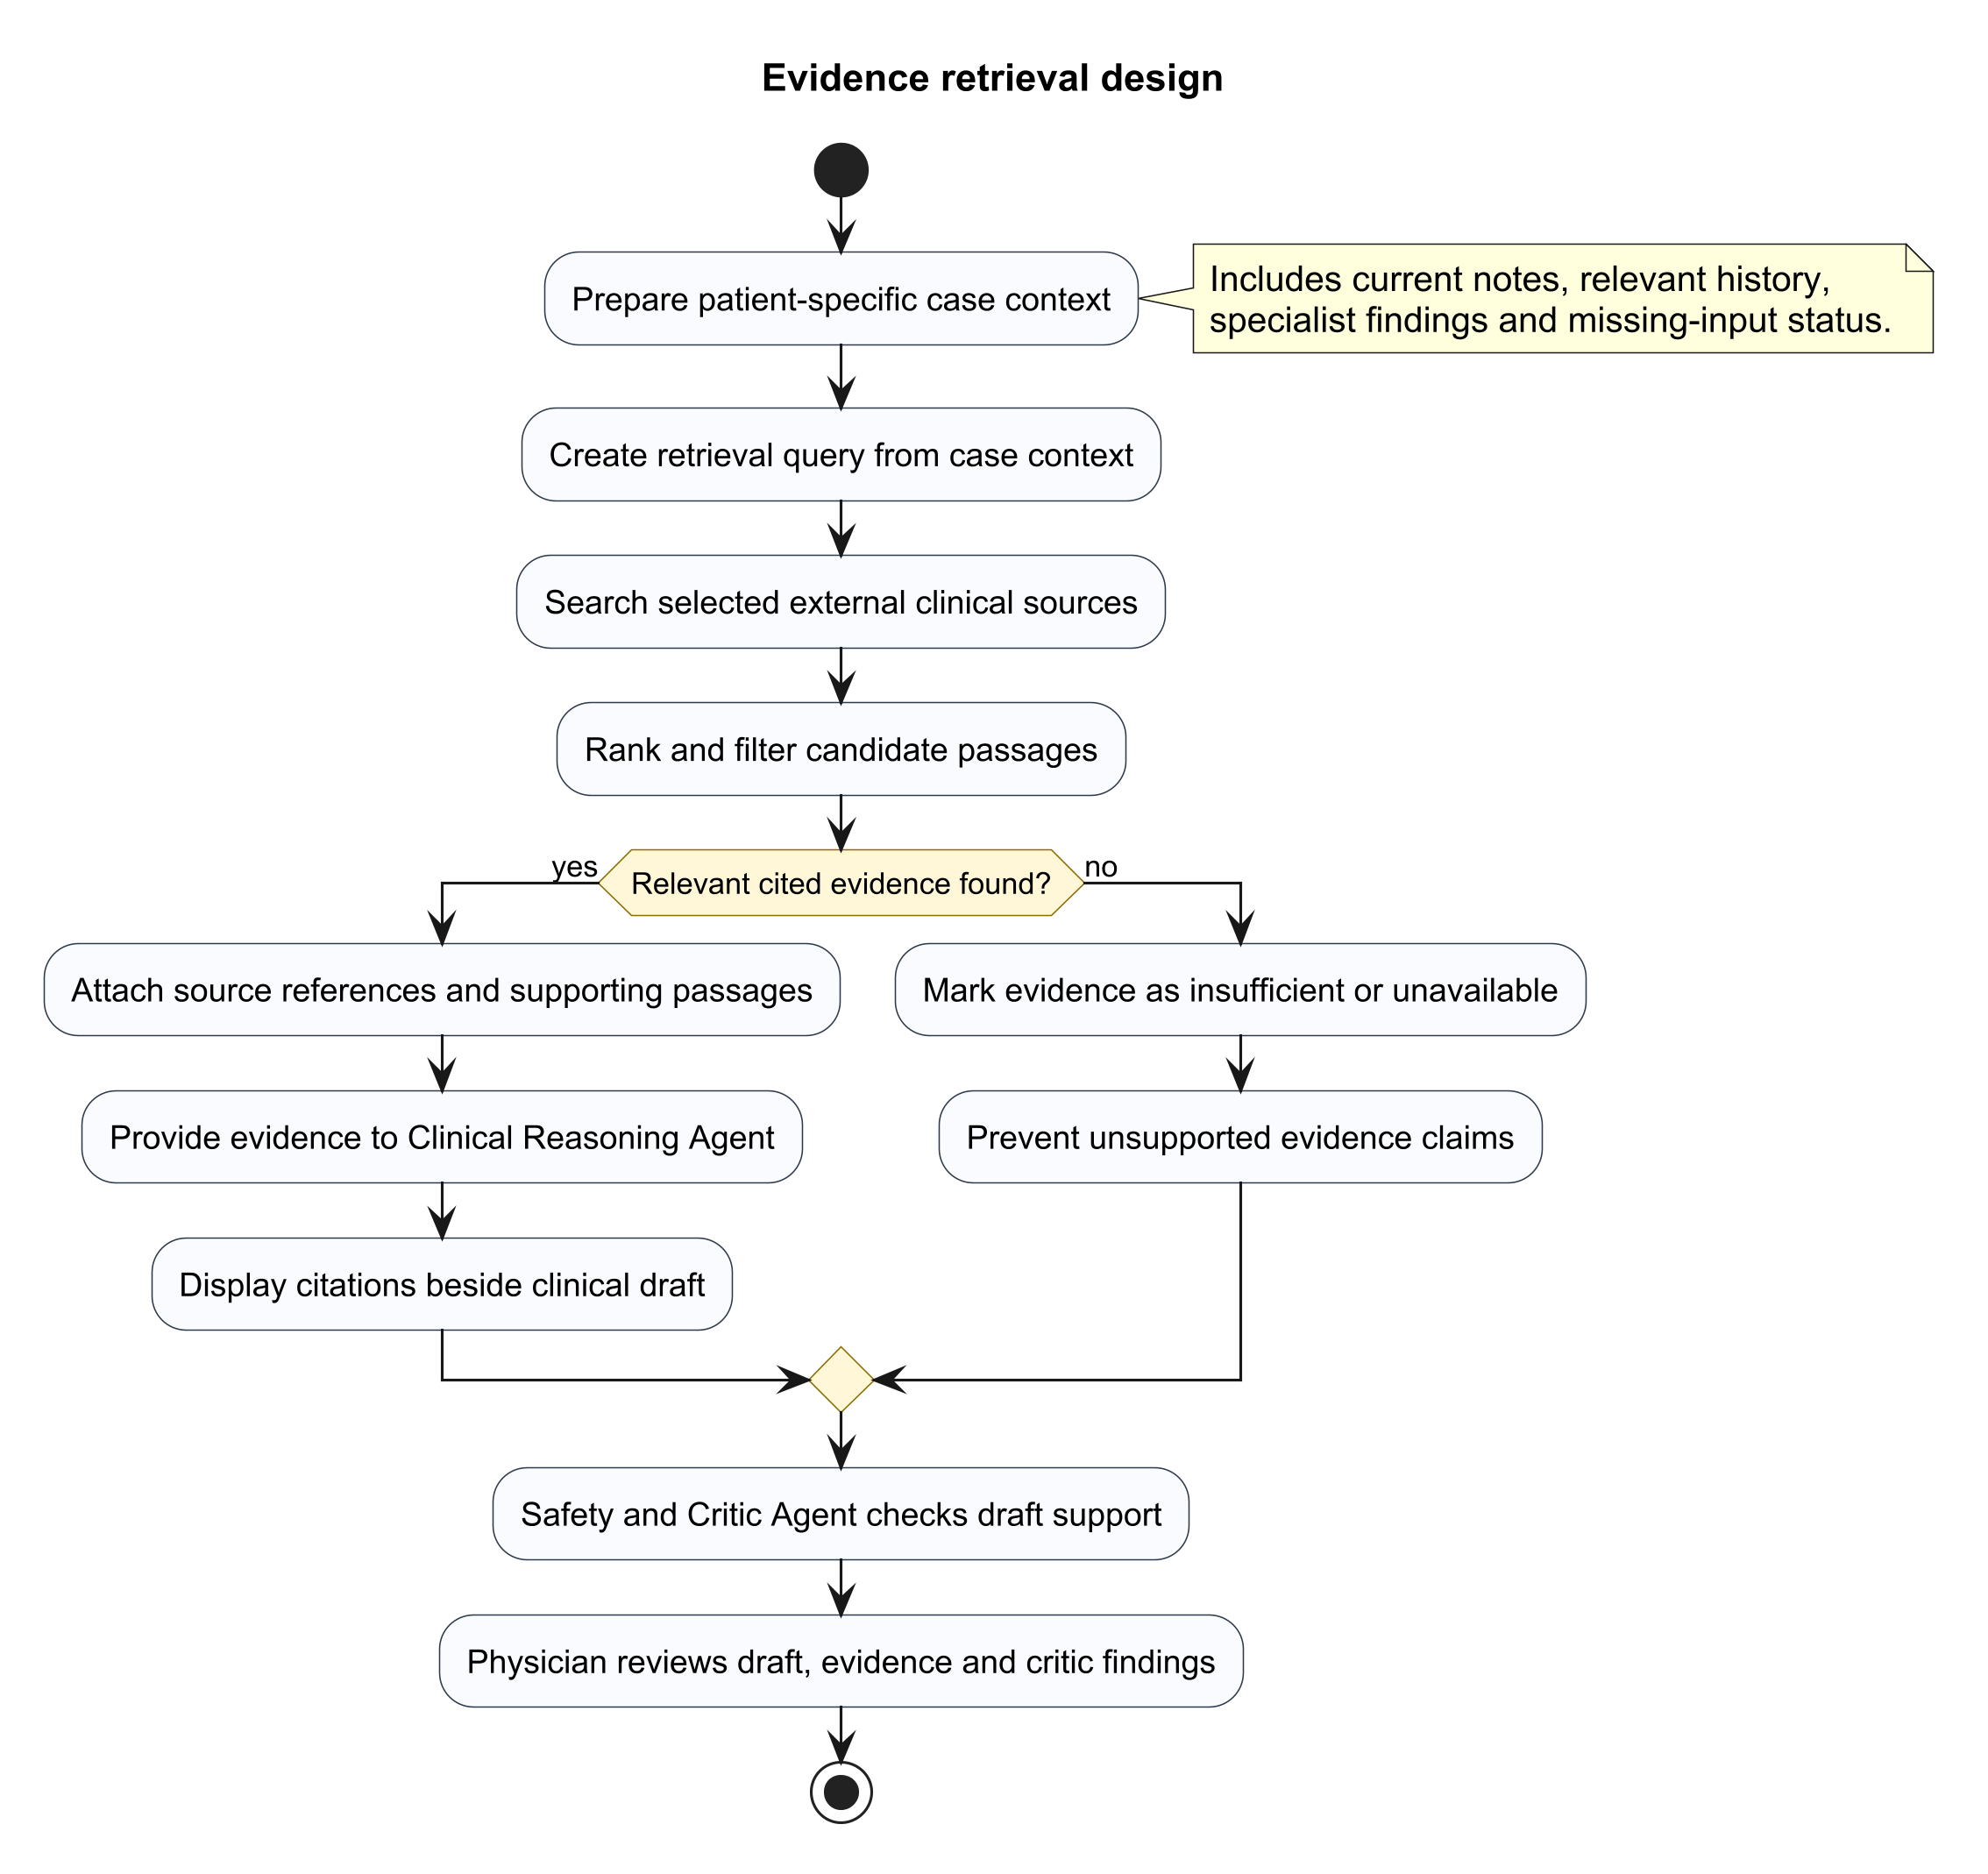
\includegraphics[width=0.92\textwidth,height=0.62\textheight,keepaspectratio]{Figures/fatima_D06_evidence_retrieval.png}
\caption{Planned evidence retrieval procedure separating patient-specific case context from external clinical sources before cited passages are attached to the clinical draft.}
\label{fig:fatima:evidence-retrieval}
\end{figure}

\section{Ablation and Evaluation Protocol}
The ablation protocol answers Zeest's evaluation questions. The comparison includes a single LLM baseline, a memory-augmented variant and the full Zeest system. The baseline receives the current case prompt only. The memory variant adds retrieved patient history, while the full system adds specialist findings, evidence retrieval and critic review. Figure~\ref{fig:fatima:ablation-protocol} shows how the same case set flows through the variants and into one assessment process. Additional contrasts examine critic and multimodal contribution where the selected cases support them. The same reference judgement process must be used for every variant. Table~\ref{tab:fatima:experiment-protocol} defines the variants and comparison controls. Outputs should be assessed for case relevance, patient-history use, evidence support, consistency with specialist findings, critic handling and physician reviewability. Metrics, sample counts, rubrics and reviewer roles remain unresolved. Possible measures include agreement with a reference judgement, citation relevance, unsupported-claim count, error categories and physician review effort. Each run should retain its configuration and output, and cases should not change between variants except for intentionally withheld inputs.

\begin{figure}[htbp]
\centering
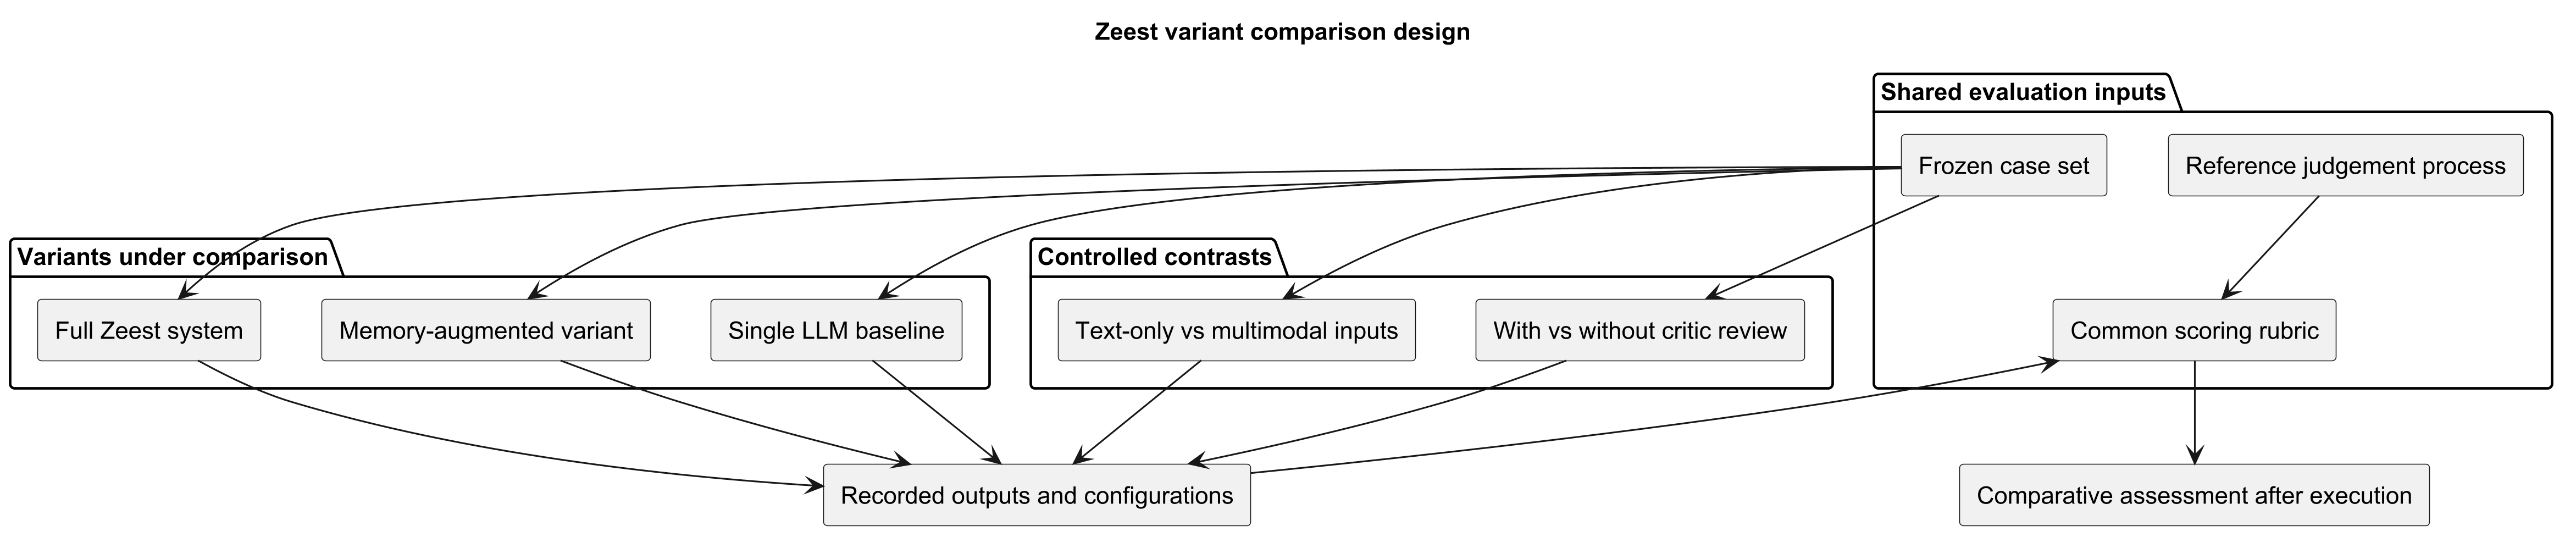
\includegraphics[width=0.96\textwidth,height=0.66\textheight,keepaspectratio]{Figures/fatima_D05_ablation_protocol.png}
\caption{Planned ablation protocol comparing a single LLM baseline, memory-augmented variant and full Zeest system using shared cases and a common reference assessment process.}
\label{fig:fatima:ablation-protocol}
\end{figure}

\begin{table}[htbp]
\centering
\scriptsize
\caption{Planned ablation and evaluation protocol for Zeest variants.}
\label{tab:fatima:experiment-protocol}
\begin{tabular}{|p{0.19\textwidth}|p{0.27\textwidth}|p{0.21\textwidth}|p{0.19\textwidth}|}
\hline
Variant or contrast & Inputs allowed & Planned assessment focus & Status \\ \hline
Single LLM baseline & Current case prompt only. & Draft relevance and unsupported claims. & Not executed. \\ \hline
Memory-augmented & Current case plus retrieved longitudinal history. & Contribution of patient memory. & Not executed. \\ \hline
Full Zeest & Case, memory, specialist findings, evidence and critic review. & Integrated workflow performance and reviewability. & Not executed. \\ \hline
Critic contrast & Full pipeline with and without critic findings. & Unsupported or contradictory output handling. & Planned control. \\ \hline
Multimodal contrast & Text-only case versus supported multimodal case. & Contribution of imaging/lab/medication findings. & Planned control. \\ \hline
Evidence contrast & Draft with and without retrieved cited passages. & Citation support and evidence relevance. & Planned control. \\ \hline
\end{tabular}
\end{table}

\section{Methodological Traceability}
The proposed methodology traces to the objectives and requirements in Chapters~2 and~4. Hybrid memory supports O1, FR18 and FR19. Transcription and note correction support O2 and FR09 through FR13. Specialist agents support O3 and FR20 through FR25. Imaging integration supports O4 and FR21, while evidence retrieval supports O5, FR27 and FR31. Clinical draft generation supports O6, FR28 and FR29. Critic review supports O7, FR30 and FR32. Physician approval, modification, rejection and audit support O8 and FR33 through FR38. The ablation protocol supports O9 and RR01 through RR04. Table~\ref{tab:fatima:method-trace} summarises this mapping so later design and evaluation work can remain aligned with the current requirements. This traceability matters because the methodology should evaluate the same workflow described in the requirements, not a different or simplified system. Later changes to IDs, selected datasets or agent responsibilities should therefore be reflected here and in Fatima's handoff before the report is considered final.

\begin{table}[htbp]
\centering
\small
\caption{Traceability between methodology stages and current requirement areas.}
\label{tab:fatima:method-trace}
\begin{tabular}{|p{0.24\textwidth}|p{0.28\textwidth}|p{0.34\textwidth}|}
\hline
Method stage & Related Chapter 4 IDs & Planned verification \\ \hline
Case preparation & FR04--FR17 & Check patient, encounter and source associations. \\ \hline
Hybrid memory retrieval & FR18--FR20 & Compare retrieved history against selected cases. \\ \hline
Specialist analysis & FR21--FR25 & Check input-specific findings and failures. \\ \hline
Evidence retrieval & FR27, FR31 & Assess citation relevance and passage support. \\ \hline
Clinical draft and critic & FR28--FR32 & Review draft consistency and critic findings. \\ \hline
Physician decision workflow & FR33--FR38 & Verify revision-specific approval and audit records. \\ \hline
Ablation framework & RR01--RR04 & Compare variants using shared cases and rubric. \\ \hline
\end{tabular}
\end{table}

\section{Dependencies and Open Method Decisions}
The methodology has unresolved dependencies before implementation and evaluation. The clinical domain must match available data, permitted use and an existing validated model. The transcription component, embedding model, evidence corpus, medication resource and LLM configuration remain to be selected. The LangGraph and Google ADK responsibility split remains a Chapter~6 design decision. Evaluation also needs reference judgements, reviewer roles, sample size, rubric and thresholds. These dependencies are important because they determine whether a case can be used, which modalities can be compared and how outputs should be judged. They also prevent the report from presenting design assumptions as completed results. This chapter therefore provides a structured plan without pretending those choices are complete. The open decisions should be closed before implementation claims or numerical evaluation results are added to the report, and any selected resource should be recorded with its permitted use and limitations. Keeping these items visible helps the team coordinate later design, testing and writing work.

\section{Conclusion}
In conclusion, Zeest's methodology combines case preparation, hybrid memory retrieval, specialist analysis, evidence-grounded drafting, critic review and physician decision control. It supports an R\&D investigation of whether memory, multimodal inputs, agent decomposition, evidence retrieval and critic review improve clinical draft reviewability. The figures and tables define input flow, unresolved resources and ablation comparisons. The procedure keeps the generated output as a draft until the physician approves, modifies or rejects it, preserving the approval boundary established in the requirements. Because the prototype is unbuilt, the chapter separates procedure from outcomes. Future work must confirm resources, implement the pipeline, execute comparisons and report measured findings with limitations. This structure gives the team a method for moving from the proposal and requirements toward a testable system while avoiding unsupported claims about clinical performance, dataset access or completed integration. It also helps later chapters and reviews check whether the design remains consistent with the planned evaluation.

\endgroup
%
% Owner: Member C (Eesha Irfan).
% Local font encoding restores the template's Times regular/bold faces under XeTeX.
\begingroup
\renewcommand{\encodingdefault}{T1}
\fontencoding{T1}\selectfont
\chapter{High-Level and Low-Level Design}

System design translates requirements into component responsibilities, interfaces and information relationships. The following sections present architectural decisions, subsystem interactions, structural models and behavioural flows, showing how data and control move between the application and its supporting services.

\section{System Overview}

The physician workspace presents patient history, editable consultation notes, specialist findings and clinical drafts in a connected encounter context. Application services validate account access and check that the patient belongs to the requesting physician before retrieving or processing related records. Behind these services, eight agents divide patient-memory retrieval, case preparation, imaging, laboratory processing, medication review, evidence retrieval, clinical reasoning and critic review. Their outputs retain source identifiers and processing states so incomplete analysis does not become an apparent finding. PostgreSQL stores account, encounter, revision and decision relationships, while pgvector supports semantic retrieval over authorised sources. Generated content remains a draft until the physician accepts its reviewed revision. Modification creates a pending revision, and rejection retains the action without creating an accepted decision. Audit records connect each review action to its actor, time and encounter. Research outputs remain separate from accepted decisions even when an evaluation uses the same encounter context.

\section{Design Considerations}

Component boundaries must accommodate different clinical representations without losing patient ownership or source context. Consultation audio needs an incremental capture path, imaging requires model-compatible preparation, and laboratory and medication information require interpretable structured inputs. External model or knowledge services can fail independently, so their status and errors must remain visible to the application. Historical retrieval must distinguish source observations from accepted decisions and prevent another physician's records from entering the case. Draft preparation needs revision-specific evidence and critic findings, while approval requires the accepted content to match the saved revision. These concerns guide the division between interface, application gateway, orchestration, analytical services and persistence. Design choices need to support controlled research comparisons without treating components as automatically beneficial. Numerical latency limits, hardware capacity, model selection and resource coverage depend on the eventual environment. Consequently, the design specifies responsibilities and failure boundaries while leaving configuration-dependent values to documented selection and measurement.

\subsection{Assumptions and Dependencies}

The direct clinical user is a physician who can interpret patient information and assess generated recommendations. The interface assumes a supported web browser, permission to capture consultation audio when recording is used, and connectivity to whichever processing services are selected. Patient cases are de-identified or synthetic, and each patient has one responsible physician for access control. Imaging analysis depends on a validated model whose task and input requirements match the chosen clinical domain. Transcription, embeddings, evidence retrieval and medication review depend on suitable resources and permitted use. PostgreSQL transactions and pgvector provide the relational and semantic storage capabilities. LangGraph and Google ADK are identified orchestration technologies, but their responsibility split requires an implementation decision rather than an assumed combined engine. These dependencies must be recorded with versions, configuration and limitations before comparative runs. A missing dependency should produce an identifiable unavailable state, not an invented finding or implied successful analysis.

\subsection{General Constraints}

Zeest provides clinical assistance rather than autonomous treatment or prescribing. Generated diagnoses and treatment plans remain reviewable drafts, and no agent can create an accepted decision through inference alone. Account and ownership checks govern every clinical read and processing request, including related inputs, drafts and audit actions. Development uses permitted de-identified or synthetic cases; this restriction does not establish regulatory approval or suitability for real clinical deployment. Existing imaging models define their own tasks, and unsupported inputs must be rejected or shown as unavailable. Computational requirements depend on the selected services and case collection, so the architecture cannot claim guaranteed throughput or query latency. Saved input and draft revisions preserve provenance across corrections and review. The same restrictions apply to evaluation configurations: cases, source permissions and reference procedures must be documented. Restrictions apply to all analytical paths, including failed requests and partially completed cases that remain available for physician inspection.

\subsection{Goals and Guidelines}

The design prioritises understandable context, traceable sources, physician control and maintainable component interfaces. Patient and encounter identifiers remain available throughout the workflow so that an operation cannot silently act on a different case. Clinical inputs, specialist findings, retrieved passages, critic findings and generated drafts have representations and display states. Approval controls identify the reviewed revision, while modification and rejection preserve their separate consequences. Analytical components exchange typed information with source references and error status rather than relying on unstructured handoffs alone. Compatible models can be replaced through adapters after their inputs and outputs are checked against these contracts. Failure handling should expose unavailable or incomplete stages without manufacturing clinical conclusions. Evidence retrieval and critic review support inspection but do not guarantee correctness or eliminate hallucinations. Research configurations preserve the same case definitions and assessment process across comparisons. Their value depends on verified behaviour rather than the number of connected components.

\subsection{ Development Methods}

Development follows the requirements, use-case definitions and logical data relationships established in Chapter~4. The initial work defines component contracts, account ownership checks and input and draft revisions before connecting model services. Small integration stages then establish patient navigation, consultation notes, specialist processing, evidence retrieval and the review boundary. Structural and behavioural diagrams describe responsibilities, messages and permitted state transitions, while test cases examine normal operations and rejected requests. Changes to an analytical component must preserve patient, encounter and source associations and expose any new input restrictions. Methodological comparisons use configurations so architecture changes can be distinguished from changes to cases or assessment conditions. The process keeps resource selection explicit: candidate datasets, knowledge sources and models require permission and domain checks before use. Implementation claims must follow working integration, and performance claims must follow measurements. The saved configuration identifies which resources and case restrictions governed each integration or evaluation run.

\section{System Architecture}

Figure~\ref{fig:esha:d07} separates the physician interface, application gateway, agent orchestration and supporting services. Next.js provides the web interface, and FastAPI provides the Python application boundary.~\cite{zeestC:nextjs,zeestC:fastapi} The gateway handles authentication, patient ownership, validated requests and revision-aware decision operations before dispatching analytical work. LangGraph and Google ADK inform the orchestration design; their exact division remains an implementation choice.~\cite{zeestB:langgraph,zeestB:googleadk} Model adapters connect consultation transcription, existing imaging classifiers and Gemini-based reasoning without exposing internal services directly to the browser.~\cite{zeestC:pytorch,zeestC:gemini} PostgreSQL preserves relational records, and pgvector supports semantic retrieval.~\cite{zeestC:pgvector} Streaming communication serves consultation capture, while transactional requests serve saved case operations and physician decisions. Failures return status rather than implied findings. Draft preparation and accepted-decision recording follow different paths, so analytical assistance cannot bypass explicit approval. The architecture describes intended service responsibilities; deployment capacity, latency and runtime configuration require implementation and measurement.  Analytical services return source-aware outputs without acquiring authority to accept a clinical decision.

\begin{figure}[!htbp]
\centering
\includegraphics[width=\textwidth,height=0.80\textheight,keepaspectratio]{Figures/esha_D07_system_architecture.pdf}
\caption{Zeest interface, gateway, agents, analytical services and hybrid memory.}
\label{fig:esha:d07}
\end{figure}

\subsection{Subsystem Architecture}

Figure~\ref{fig:esha:d08} groups the eight agents by their contributions to case preparation, specialised analysis and draft review. The Patient Memory Agent retrieves source-aware history, and the Clinical Case Agent combines it with current saved inputs. Imaging, Laboratory and Medication Safety agents return findings or explicit failure states for supported inputs. The Evidence and RAG Agent supplies cited passages, the Clinical Reasoning Agent creates a diagnosis and treatment draft, and the Safety and Critic Agent identifies concerns before presentation. Table~\ref{tab:esha:contracts} defines these handoffs. Figure~\ref{fig:esha:d10} follows consultation capture through note correction, analysis and physician presentation; Figure~\ref{fig:esha:d12} follows modification, approval and rejection through persistence. Independent analyses may run concurrently where their dependencies permit, but downstream reasoning must identify incomplete stages. Authorised input revisions and approved decisions can supply semantic memory; pending drafts cannot enter it as accepted clinical facts. These contracts preserve the distinction between preparation, recommendations and recorded decisions. Their outputs require verification.

\begin{figure}[!htbp]
\centering
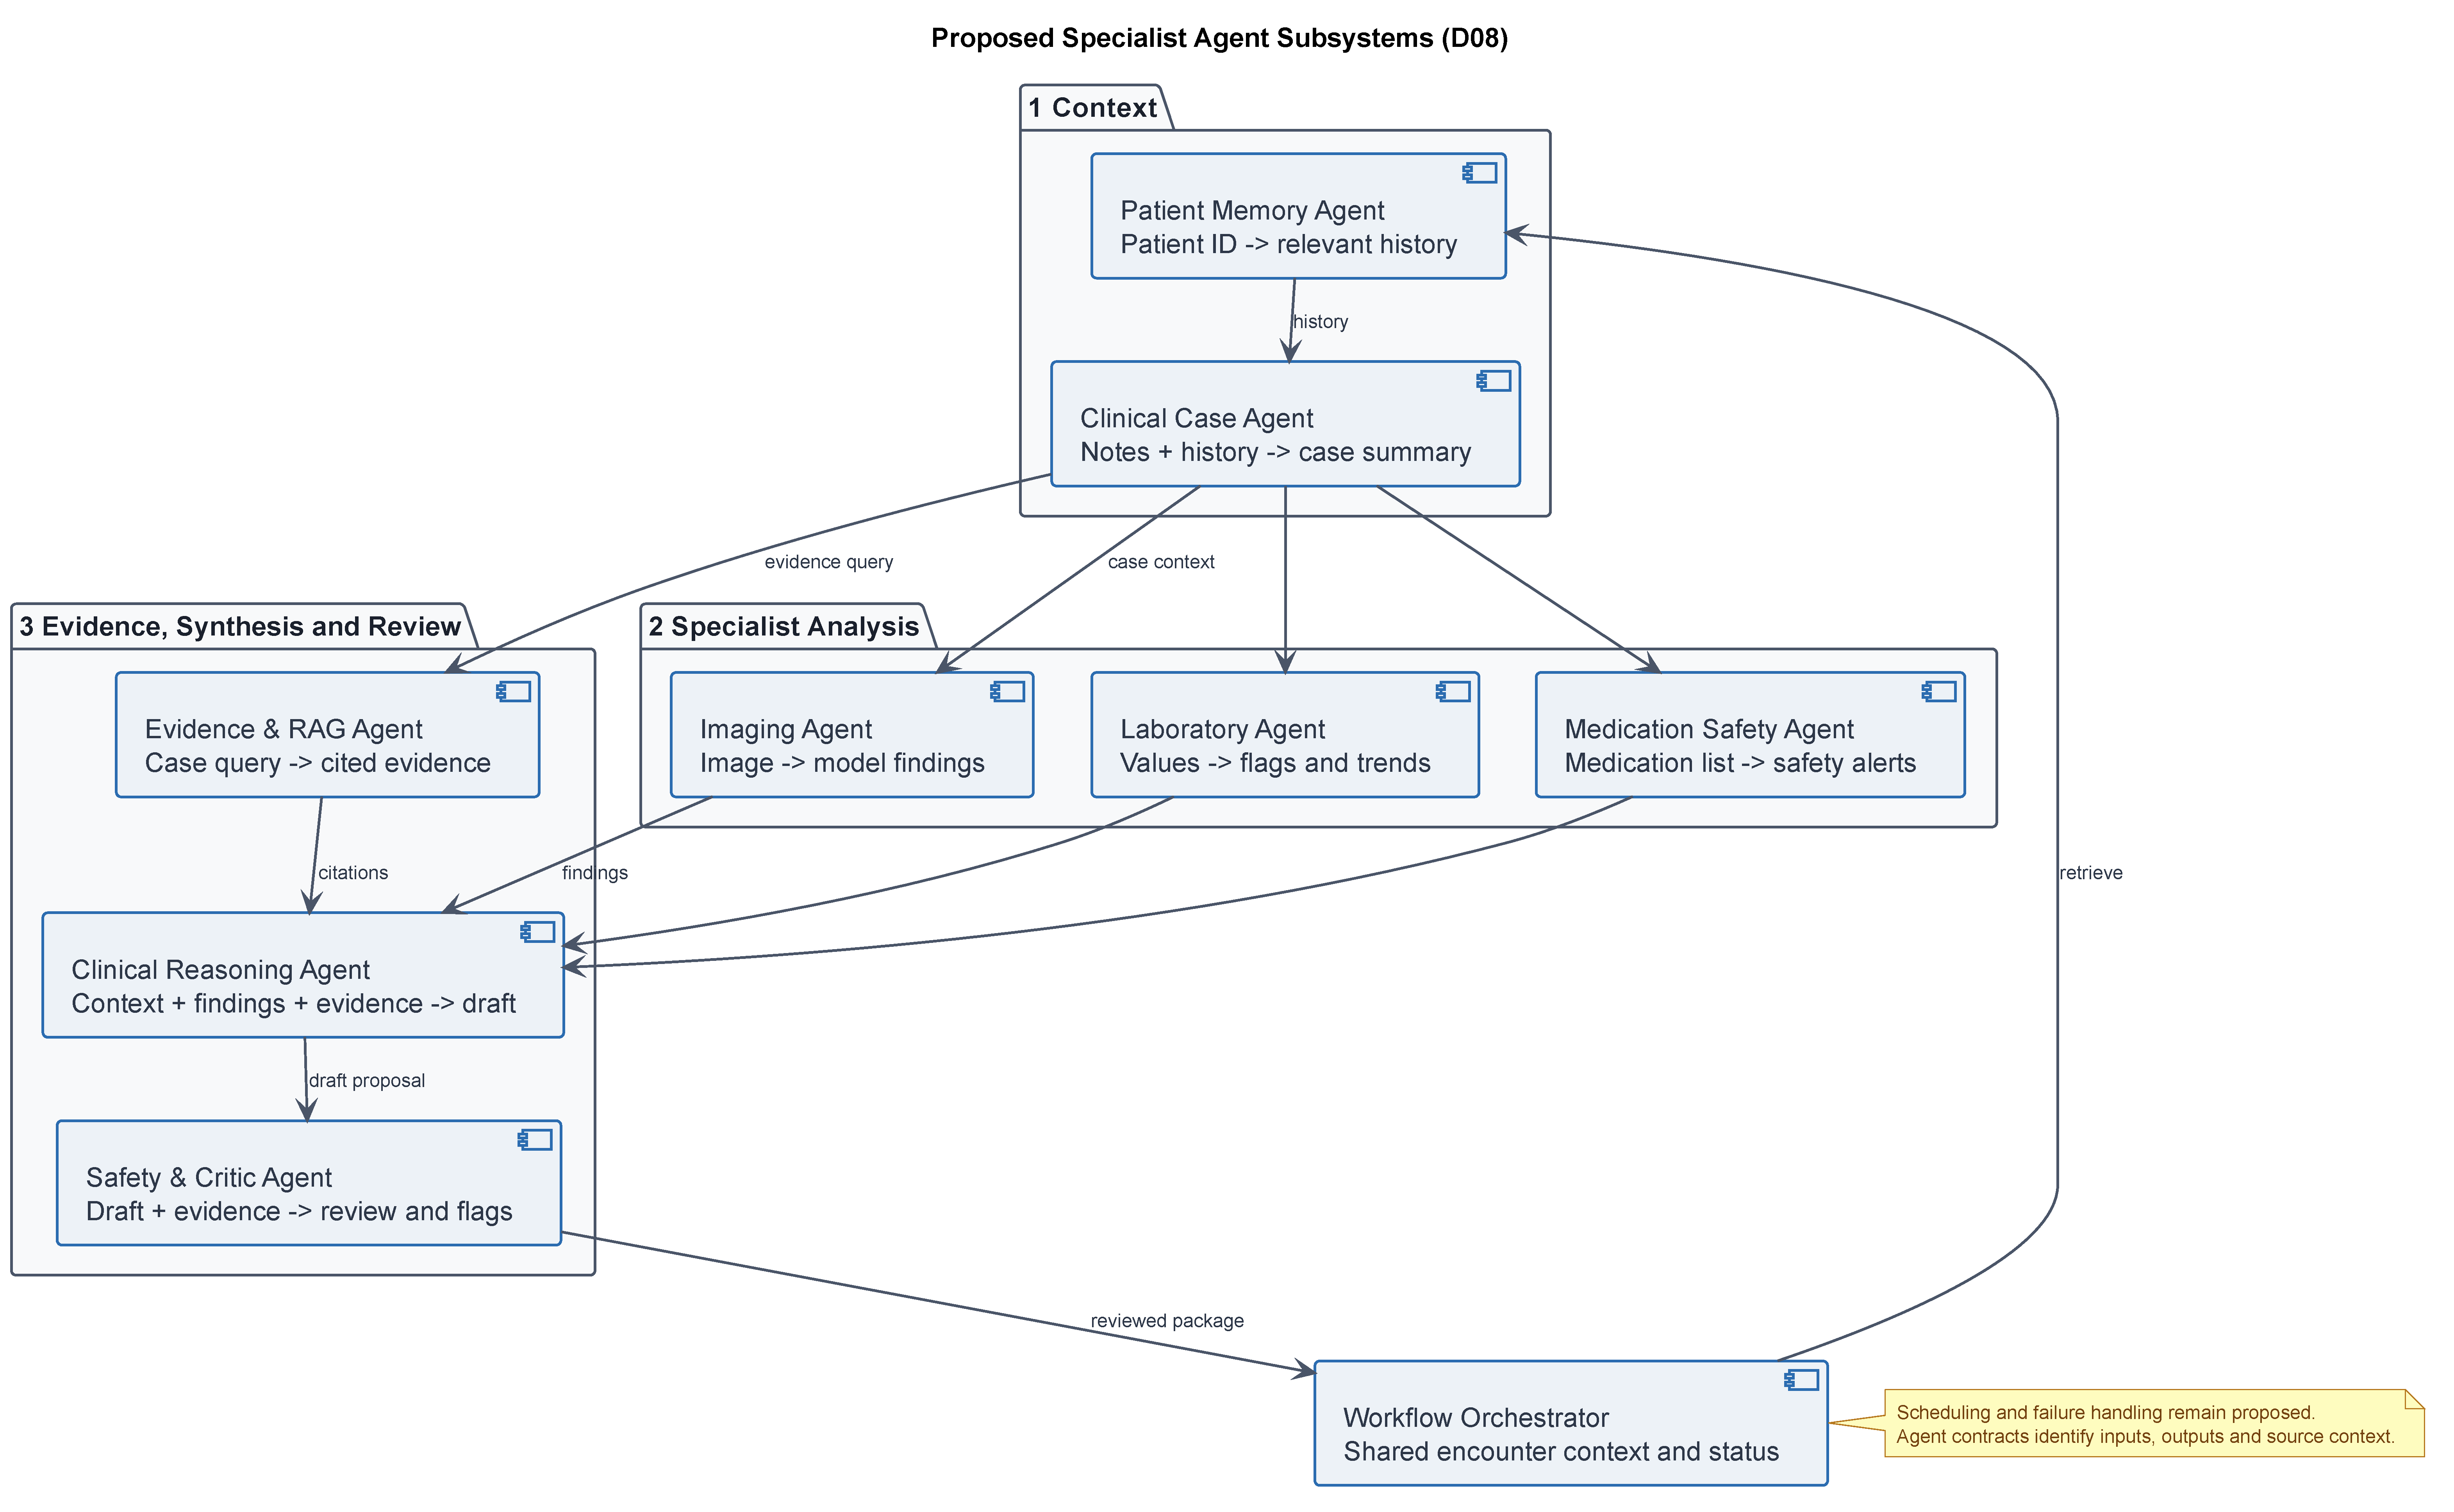
\includegraphics[width=\textwidth,height=0.80\textheight,keepaspectratio]{Figures/esha_D08_agent_subsystems.pdf}
\caption{Eight specialist agents and their case-processing handoffs.}
\label{fig:esha:d08}
\end{figure}

\begin{reporttable}
\centering
\small
\caption{Proposed specialist agent input, output, persistence and recipient contracts .}
\label{tab:esha:contracts}
\begin{tabular}{|p{0.18\textwidth}|p{0.22\textwidth}|p{0.245\textwidth}|p{0.245\textwidth}|}
\hline
Agent Name & Primary Inputs & Primary Outputs & Storage \& Recipient \\ \hline
Patient Memory Agent & \texttt{patient\_id}, encounter context & Relational history, top-$k$ semantic memories & PostgreSQL/pgvector; Orchestrator \\ \hline
Clinical Case Agent & Notes, multimodal data, retrieved history & Consolidated case representation & Working memory cache; Specialist agents \\ \hline
Imaging Agent & Radiological image tensor / file reference & Predicted pathology classes, confidence scores & Working cache; Reasoning Agent \\ \hline
Laboratory Agent & Laboratory panel values, reference ranges & Abnormal biomarker flags, trajectory trends & Working cache; Reasoning Agent \\ \hline
Medication Safety Agent & Active prescriptions, candidate drugs & Drug-drug interactions, contraindication alerts & Knowledge base; Reasoning Agent \\ \hline
Evidence \& RAG Agent & Diagnostic keywords, clinical hypotheses & Cited guideline passages, source identifiers & pgvector vector index; Reasoning Agent \\ \hline
Clinical Reasoning Agent & Consolidated case, specialist findings, evidence & Differential diagnosis draft, treatment plan & Gemini API; Safety \& Critic Agent \\ \hline
Safety \& Critic Agent & Generated draft, case context, cited evidence & Consistency evaluation, risk alerts, critique & Working cache; Presentation tier \\ \hline
\end{tabular}
\end{reporttable}

\begin{figure}[!htbp]
\centering
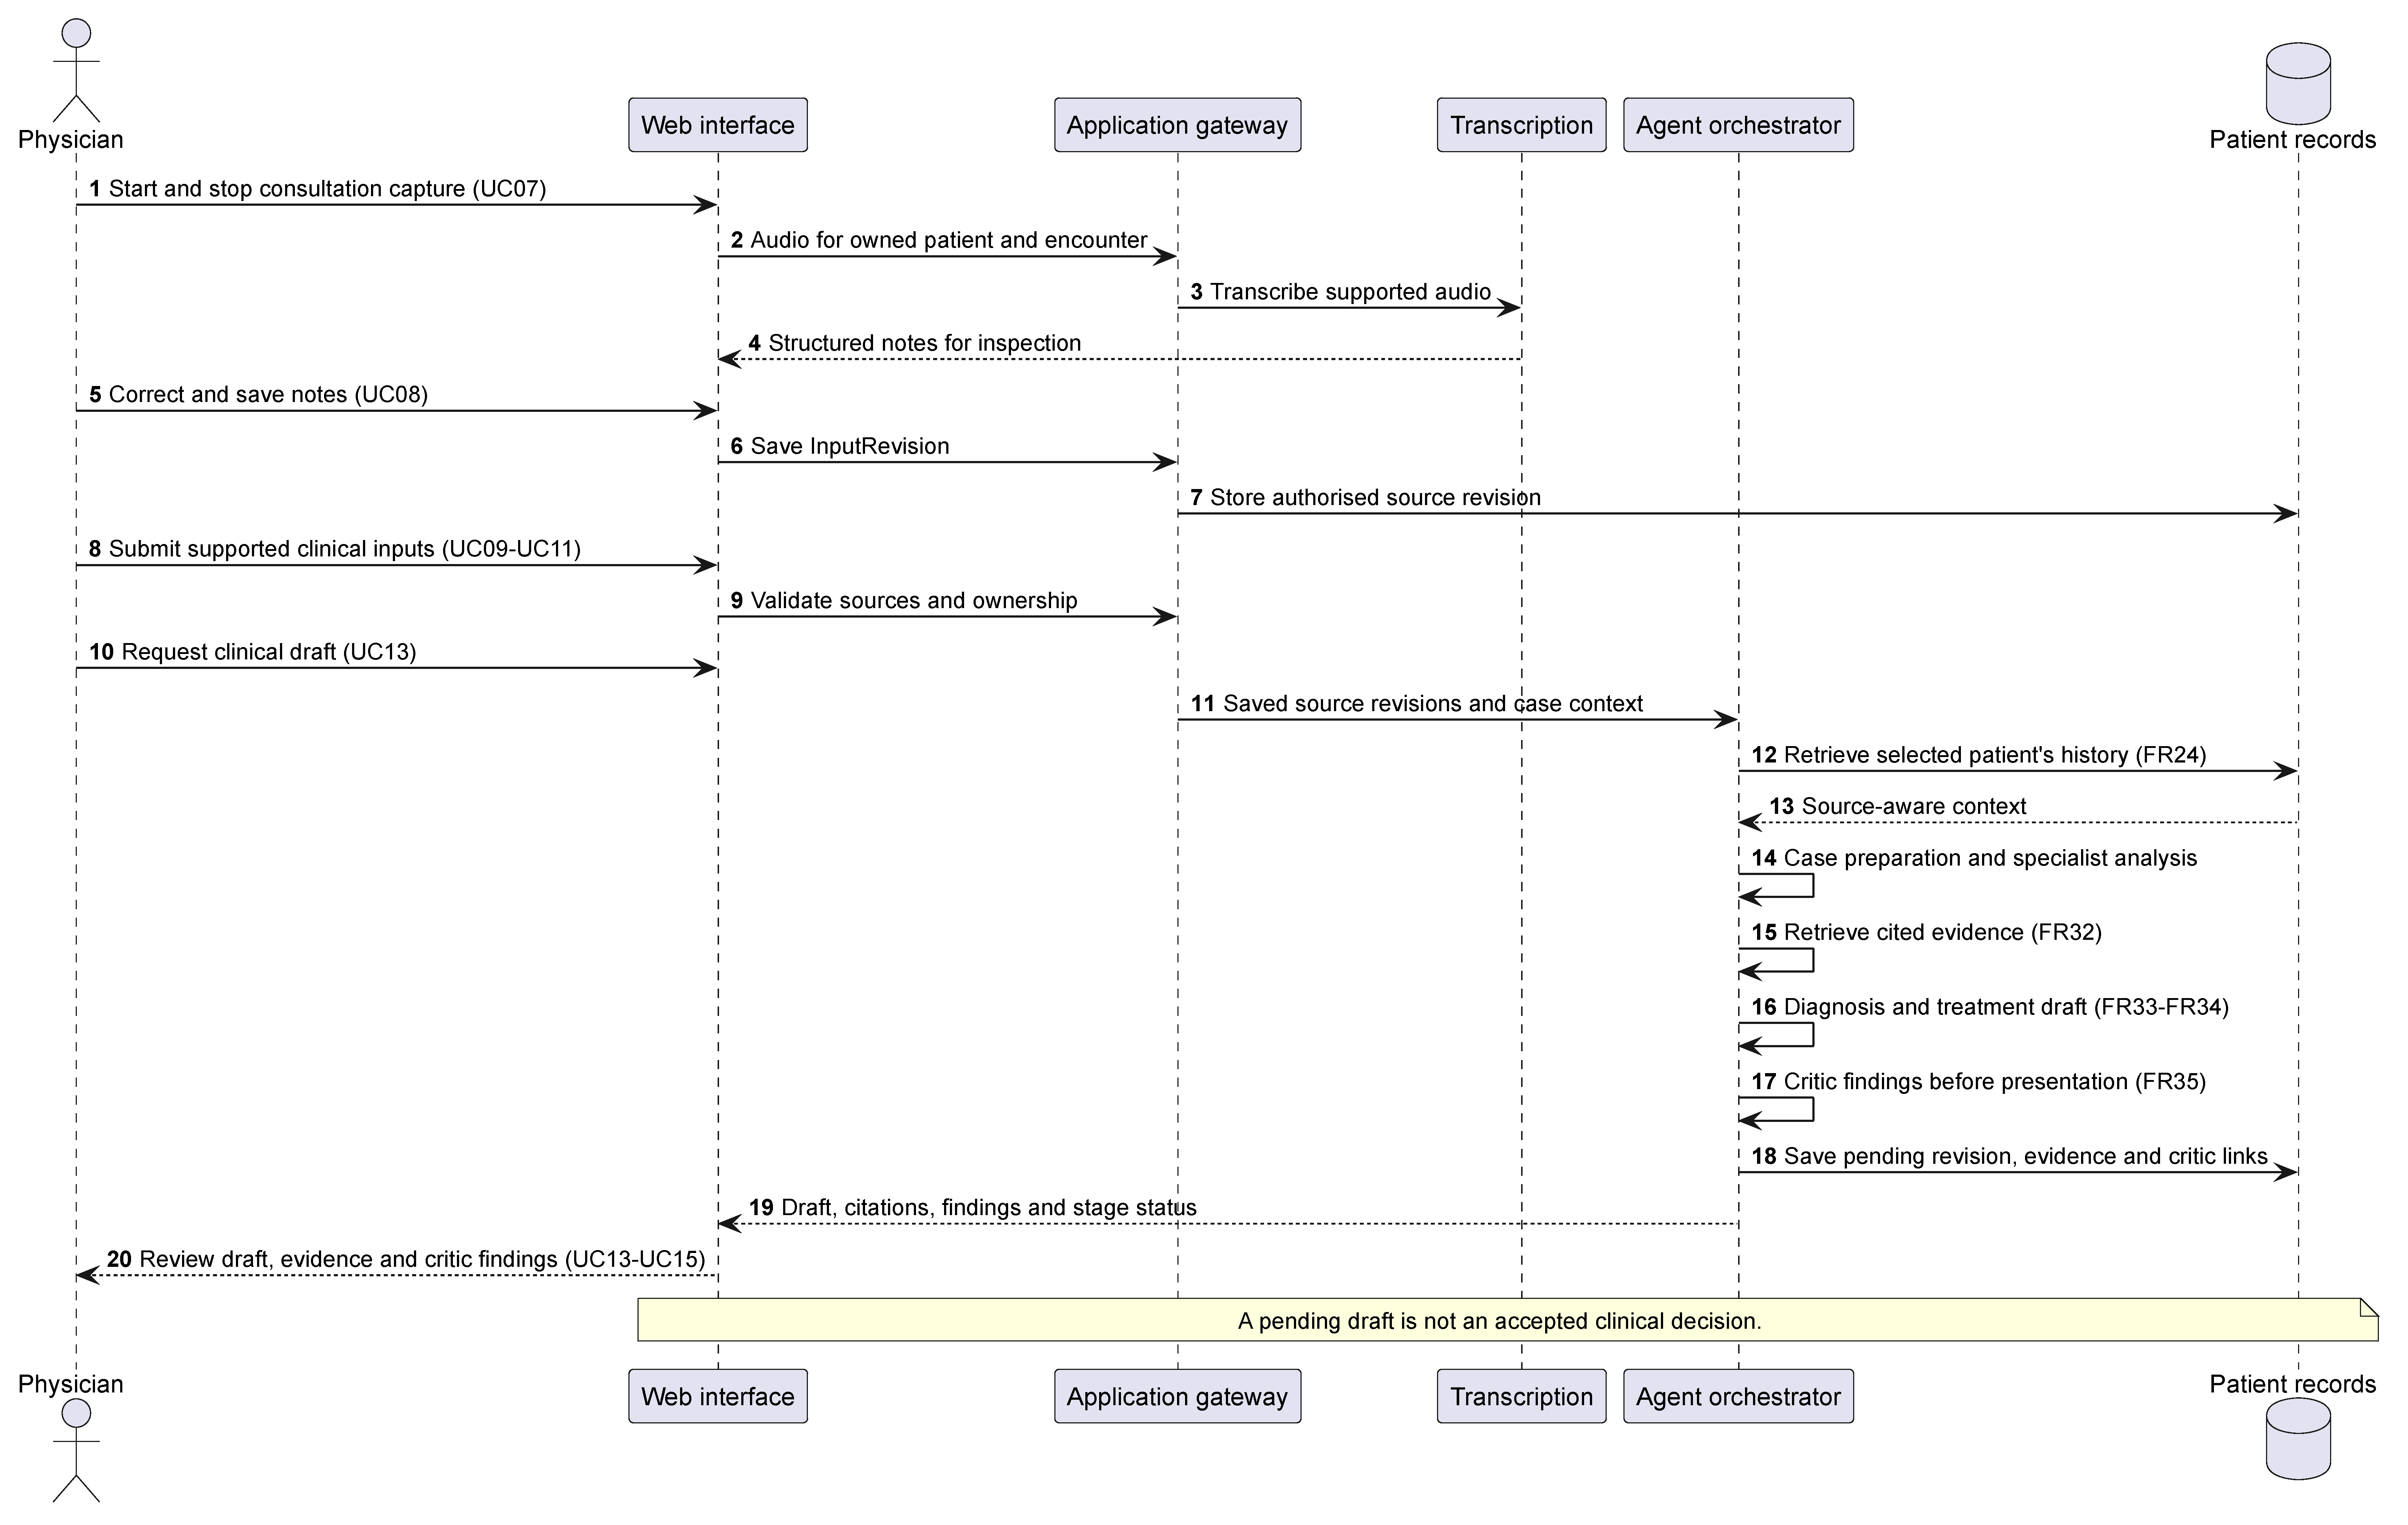
\includegraphics[width=\textwidth,height=0.80\textheight,keepaspectratio]{Figures/esha_D10_consultation_sequence.pdf}
\caption{Consultation capture, source-aware analysis and draft presentation sequence.}
\label{fig:esha:d10}
\end{figure}

\begin{figure}[!htbp]
\centering
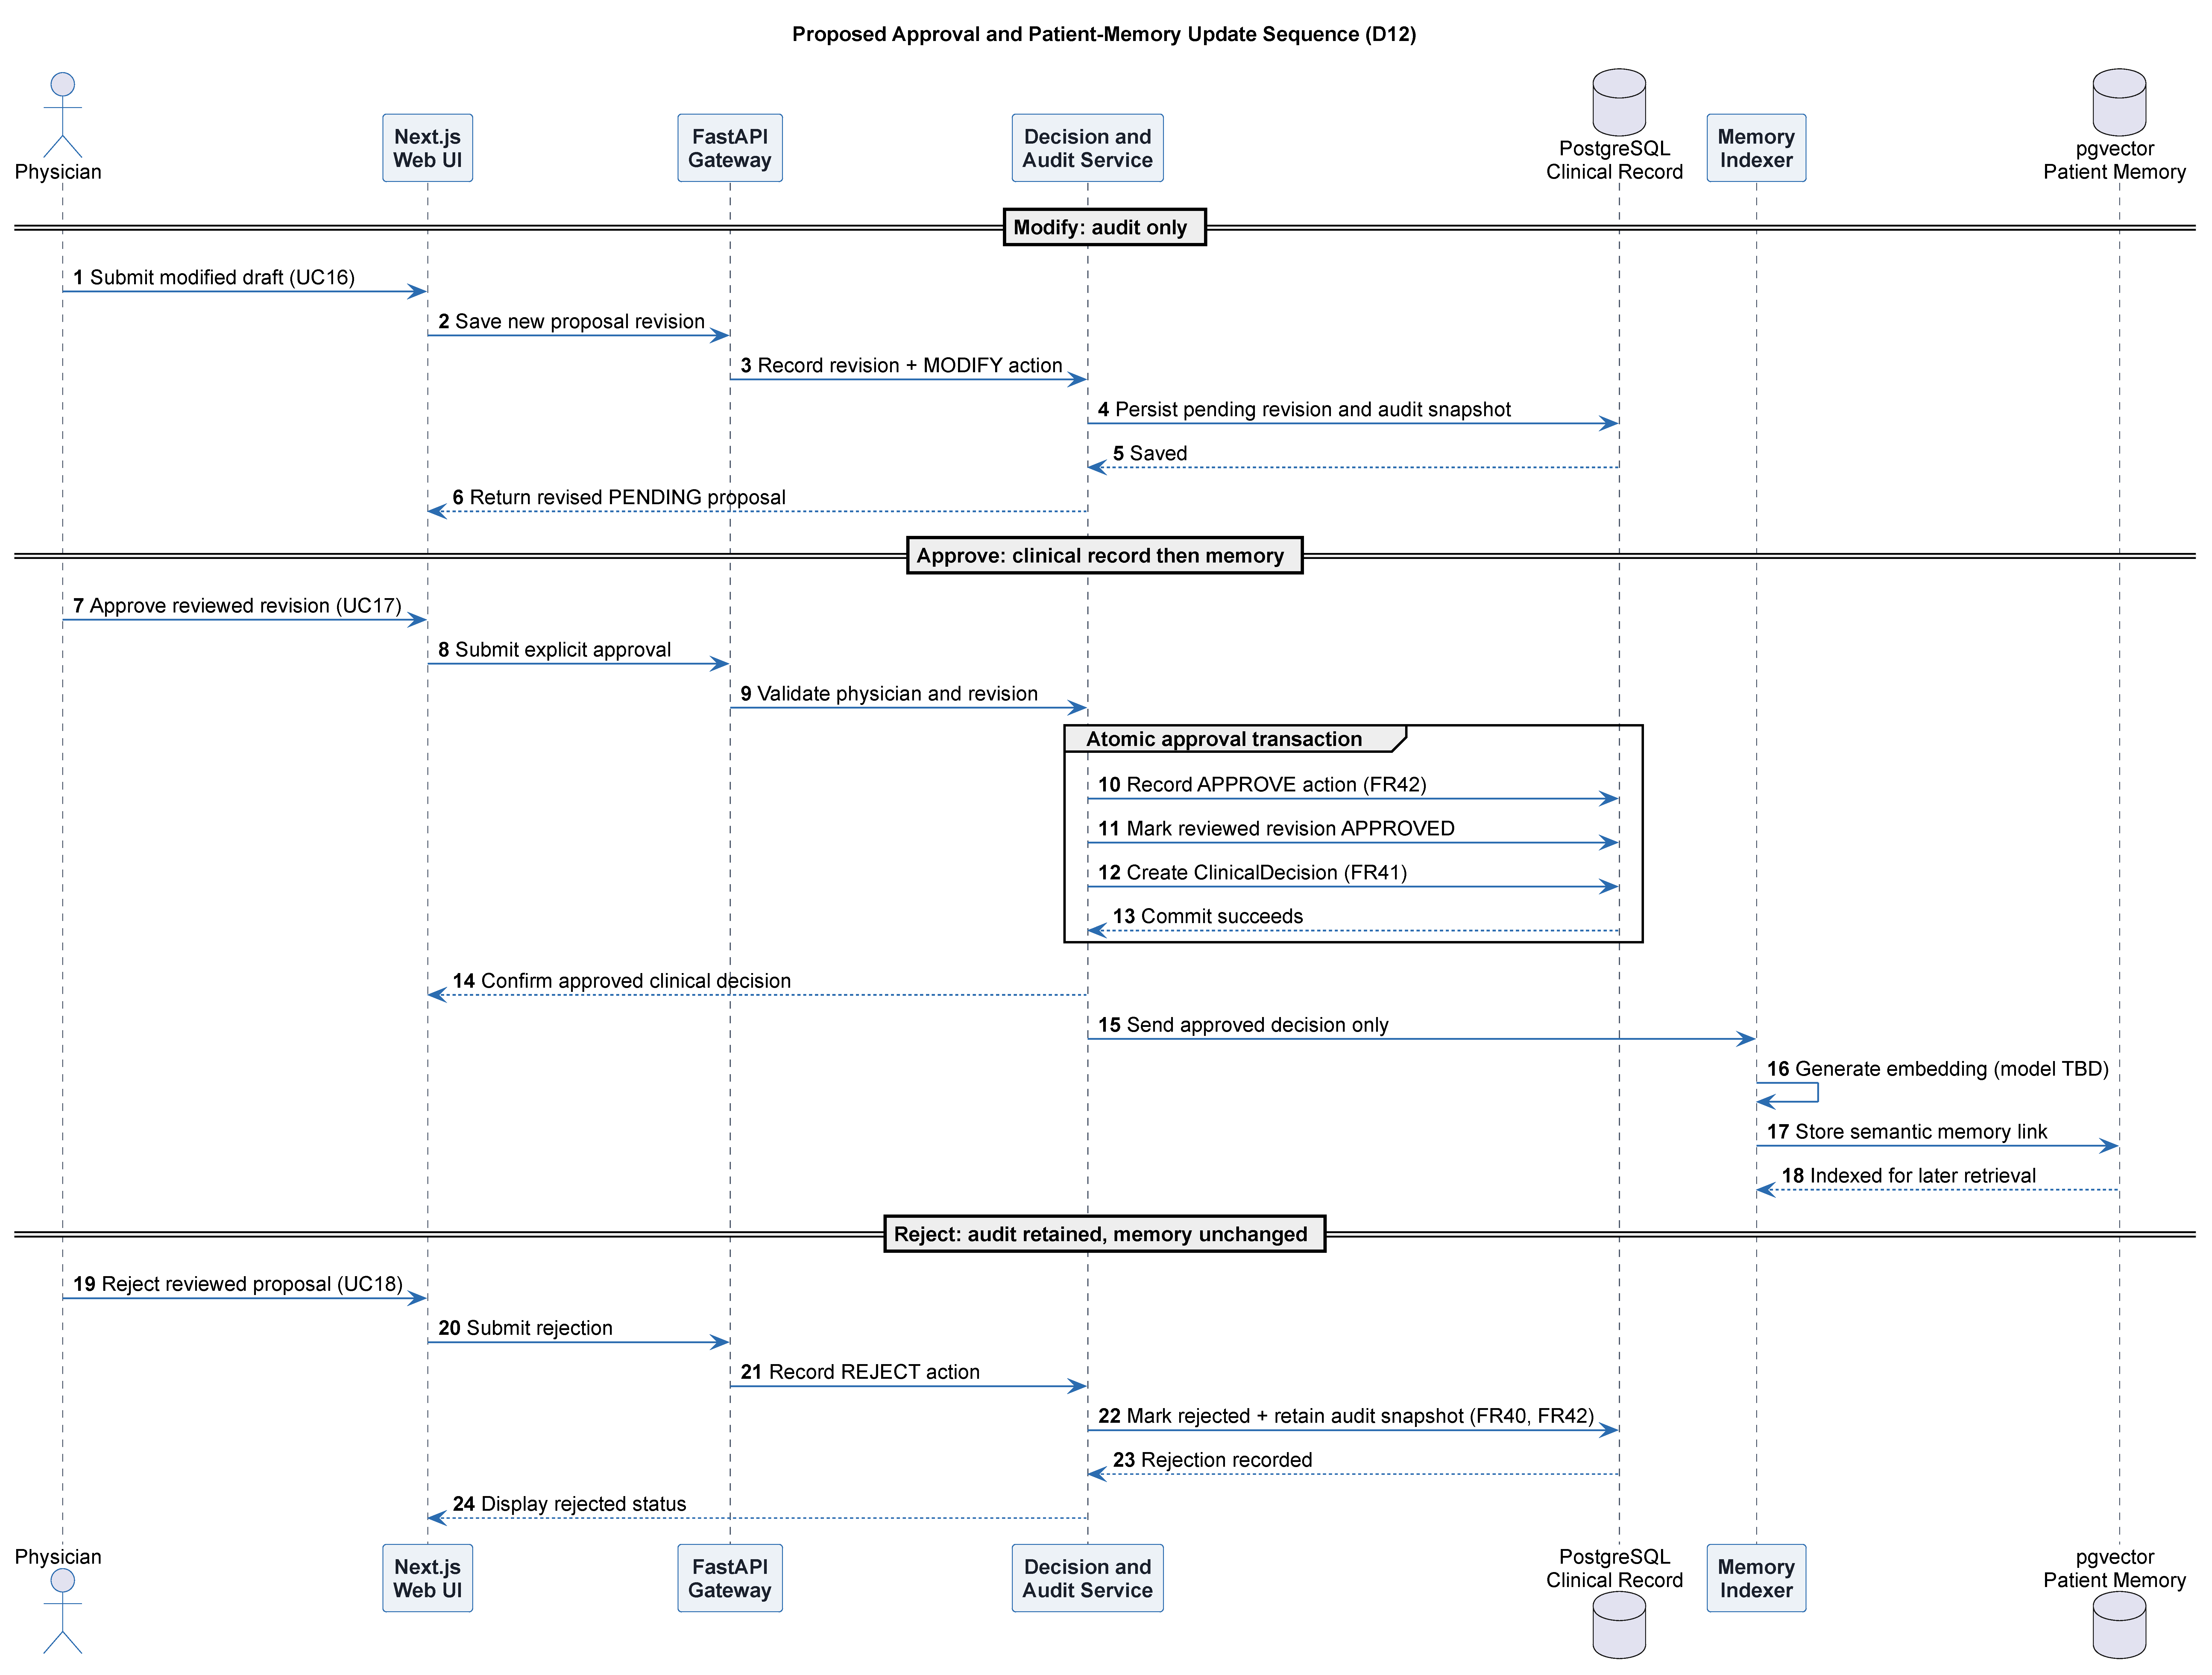
\includegraphics[width=0.96\textwidth,height=0.78\textheight,keepaspectratio]{Figures/esha_D12_memory_update_sequence.pdf}
\caption{Revision-specific physician actions, decision recording and memory indexing.}
\label{fig:esha:d12}
\end{figure}


\section{Architectural Strategies}

The architectural strategies address patient continuity, processing dependencies and accountable review rather than assuming diagnostic improvement from added components. Hybrid persistence combines explicit account, patient and encounter relationships with semantic retrieval over identifiable sources. Orchestration keeps agent responsibilities separate and coordinates their inputs before drafting. Model adapters isolate service-specific formats and errors, while transactional application services govern approval and audit recording. Table~\ref{tab:esha:decisions} records the supported technology choices, trade-offs and configuration decisions that remain open. These strategies support controlled evaluation: a simpler variant can withhold a component while retaining the same case definition and reference process. Independent processing may use asynchronous execution, but dependencies must be respected and failed analyses must remain visible. No strategy establishes guaranteed throughput, clinical safety or regulatory compliance. Its value must be assessed through implementation checks and comparative runs. The design connects engineering choices to testable behaviour while preserving the physician's responsibility for every accepted revision.

\subsection{Hybrid Relational and Vector Memory Persistence}

PostgreSQL preserves physician ownership, patient and encounter associations, input revisions, draft revisions, evidence links, review actions and accepted decisions. Foreign keys and transaction boundaries support checks that related records belong to the same case and reviewed revision. Semantic memory uses pgvector representations linked to an authorised input revision or an approved decision. This distinction permits retrieval of source observations while preventing a pending or rejected draft from being treated as an accepted clinical conclusion. Retrieval returns the originating record and its context so similarity alone does not establish clinical relevance. Historical information must remain within the selected patient's ownership boundary, and observations must remain distinguishable from earlier encounters. Embedding model, dimension and indexing configuration require selection before storage and search can be evaluated. The hybrid design retains explicit relationships alongside semantic search, but its relevance and latency must be measured rather than inferred from the presence of a vector index.

\subsection{Asynchronous Agent Orchestration and Model Runtime Segregation}

The application separates case operations from analytical work that may depend on local inference or remote services. Consultation capture, saved note revisions and physician review should retain understandable states while an analysis is pending. The orchestrator starts independent specialist tasks only after the required case context is available, then combines returned findings and failure information before drafting. Dependencies determine whether a task can run concurrently; evidence retrieval must receive the information needed to form a query. Service adapters validate payloads and distinguish timeouts, rejected inputs and unavailable resources from completed results. A partial case can remain available for inspection, but missing analysis must not be silently represented as normal findings. LangGraph and Google ADK provide candidate orchestration mechanisms, with their final division during implementation. Asynchronous execution supports this separation without establishing a measured speed improvement. Stage status should remain visible while other services finish, fail or await required case information.

\begin{reporttable}
\centering
\small
\caption{Architectural design decisions, supported choices, trade-offs and unresolved options .}
\label{tab:esha:decisions}
\begin{tabular}{|p{0.20\textwidth}|p{0.22\textwidth}|p{0.245\textwidth}|p{0.225\textwidth}|}
\hline
Design Dimension & Proposed Choice & Architectural Trade-off & Unresolved Status \\ \hline
Backend Framework & FastAPI (Python) & High-speed async I/O and native Python ML ecosystem versus separate microservices & Production server concurrency tuning TBD \\ \hline
Frontend Framework & Next.js / TypeScript & Rich React component ecosystem and streaming support versus heavier bundle size & View layout refactoring planned \\ \hline
Multi-Agent Orchestrator & LangGraph / Google ADK StateGraph & Cyclic state-graph flexibility versus increased execution graph complexity & Formal division of roles between frameworks TBD \\ \hline
Primary Reasoning Model & Google Gemini API & Advanced multimodal context window versus reliance on cloud API latency & Production model version and quotas TBD \\ \hline
Radiology Classifier & PyTorch Pre-trained Model & Validated local inference speed versus fixed diagnostic pathology label sets & Exact pre-trained model checkpoint TBD \\ \hline
Memory Storage & PostgreSQL with pgvector extension & Unified relational ACID guarantees and vector search versus dedicated vector database & Vector dimension and HNSW index tuning TBD \\ \hline
\end{tabular}
\end{reporttable}


\section{Domain Model/Class Diagram}

Figure~\ref{fig:esha:d09} presents the clinical domain classes and their associations; the complete persistence attributes are defined in Chapter~4. Physician, Patient and Encounter maintain account access, ownership and patient encounter context. ClinicalInput and InputRevision distinguish an input from its saved versions, while SpecialistFinding identifies the revision analysed. Proposal and ProposalRevision separate a draft's identity from reviewed content; ProposalInput, EvidenceItem, ProposalEvidence and CriticReview preserve its sources and assessment. PhysicianAction records the actor, revision and physician review event, and ClinicalDecision stores the explicitly accepted content. SemanticMemory links authorised source revisions or approved decisions to their representations. EvaluationCase, EvaluationRun and EvaluationOutput keep research case inputs, configurations and outputs identifiable. Application services coordinate retrieval, analysis and transactional approval rather than assigning unrestricted database writes to agents. The model aligns with the eighteen-entity dictionary while distinguishing service behaviour from stored records. Class associations specify domain entity relationships; their integrity must be verified when persistence is implemented.

\begin{figure}[!htbp]
\centering
\includegraphics[width=\textwidth,height=0.80\textheight,keepaspectratio]{Figures/esha_D09_domain_classes.pdf}
\caption{Domain classes with ownership, revision, evidence and decision associations.}
\label{fig:esha:d09}
\end{figure}


\section{Policies and Tactics}

Local policies govern account access, source handling and state transitions within the architecture. The physician's authenticated identity is checked against the selected patient before any related record is read or processed. Saved revisions preserve the clinical content used for analysis and review, while source links identify the findings and passages supporting each draft. Review actions retain their actor, time and revision; approval records matching accepted content in a transaction, and modification or rejection does not create a decision. Evidence and critic findings remain inspectable even when they identify insufficient support. Analytical errors must be returned with their stage and source context so an incomplete operation cannot appear successful. Semantic retrieval distinguishes authorised observations from approved conclusions and excludes unaccepted draft content from accepted-decision memory. These policies provide verification targets for implementation and research cases. Checks must cover incorrect ownership, stale revisions and missing evidence as well as successful workflow operations.

\subsection{Physician Review Boundary and Audit Immutability Policy}

Figure~\ref{fig:esha:d11} distinguishes pending, modified, approved and rejected draft states. Every generated draft begins pending physician review. Modification creates a saved revision and records a MODIFY action while leaving the draft unapproved. Approval requires the authenticated physician to own the patient and review the exact saved revision. A transaction records the APPROVE action, accepted revision and matching ClinicalDecision, preventing an action from accepting different content. Rejection records a REJECT action and retains the review history without creating an accepted decision. Audit entries preserve the actor, time, encounter and revision rather than replacing earlier review events. Pending and rejected revisions remain available as drafts and history, but cannot enter accepted-decision memory. Authorised clinical input revisions can still provide historical context through their separate source links. These controls define the decision boundary; concurrency, failed transactions and repeated requests must be checked during implementation to confirm that their recorded outcomes preserve the required relationships.

\begin{figure}[!htbp]
\centering
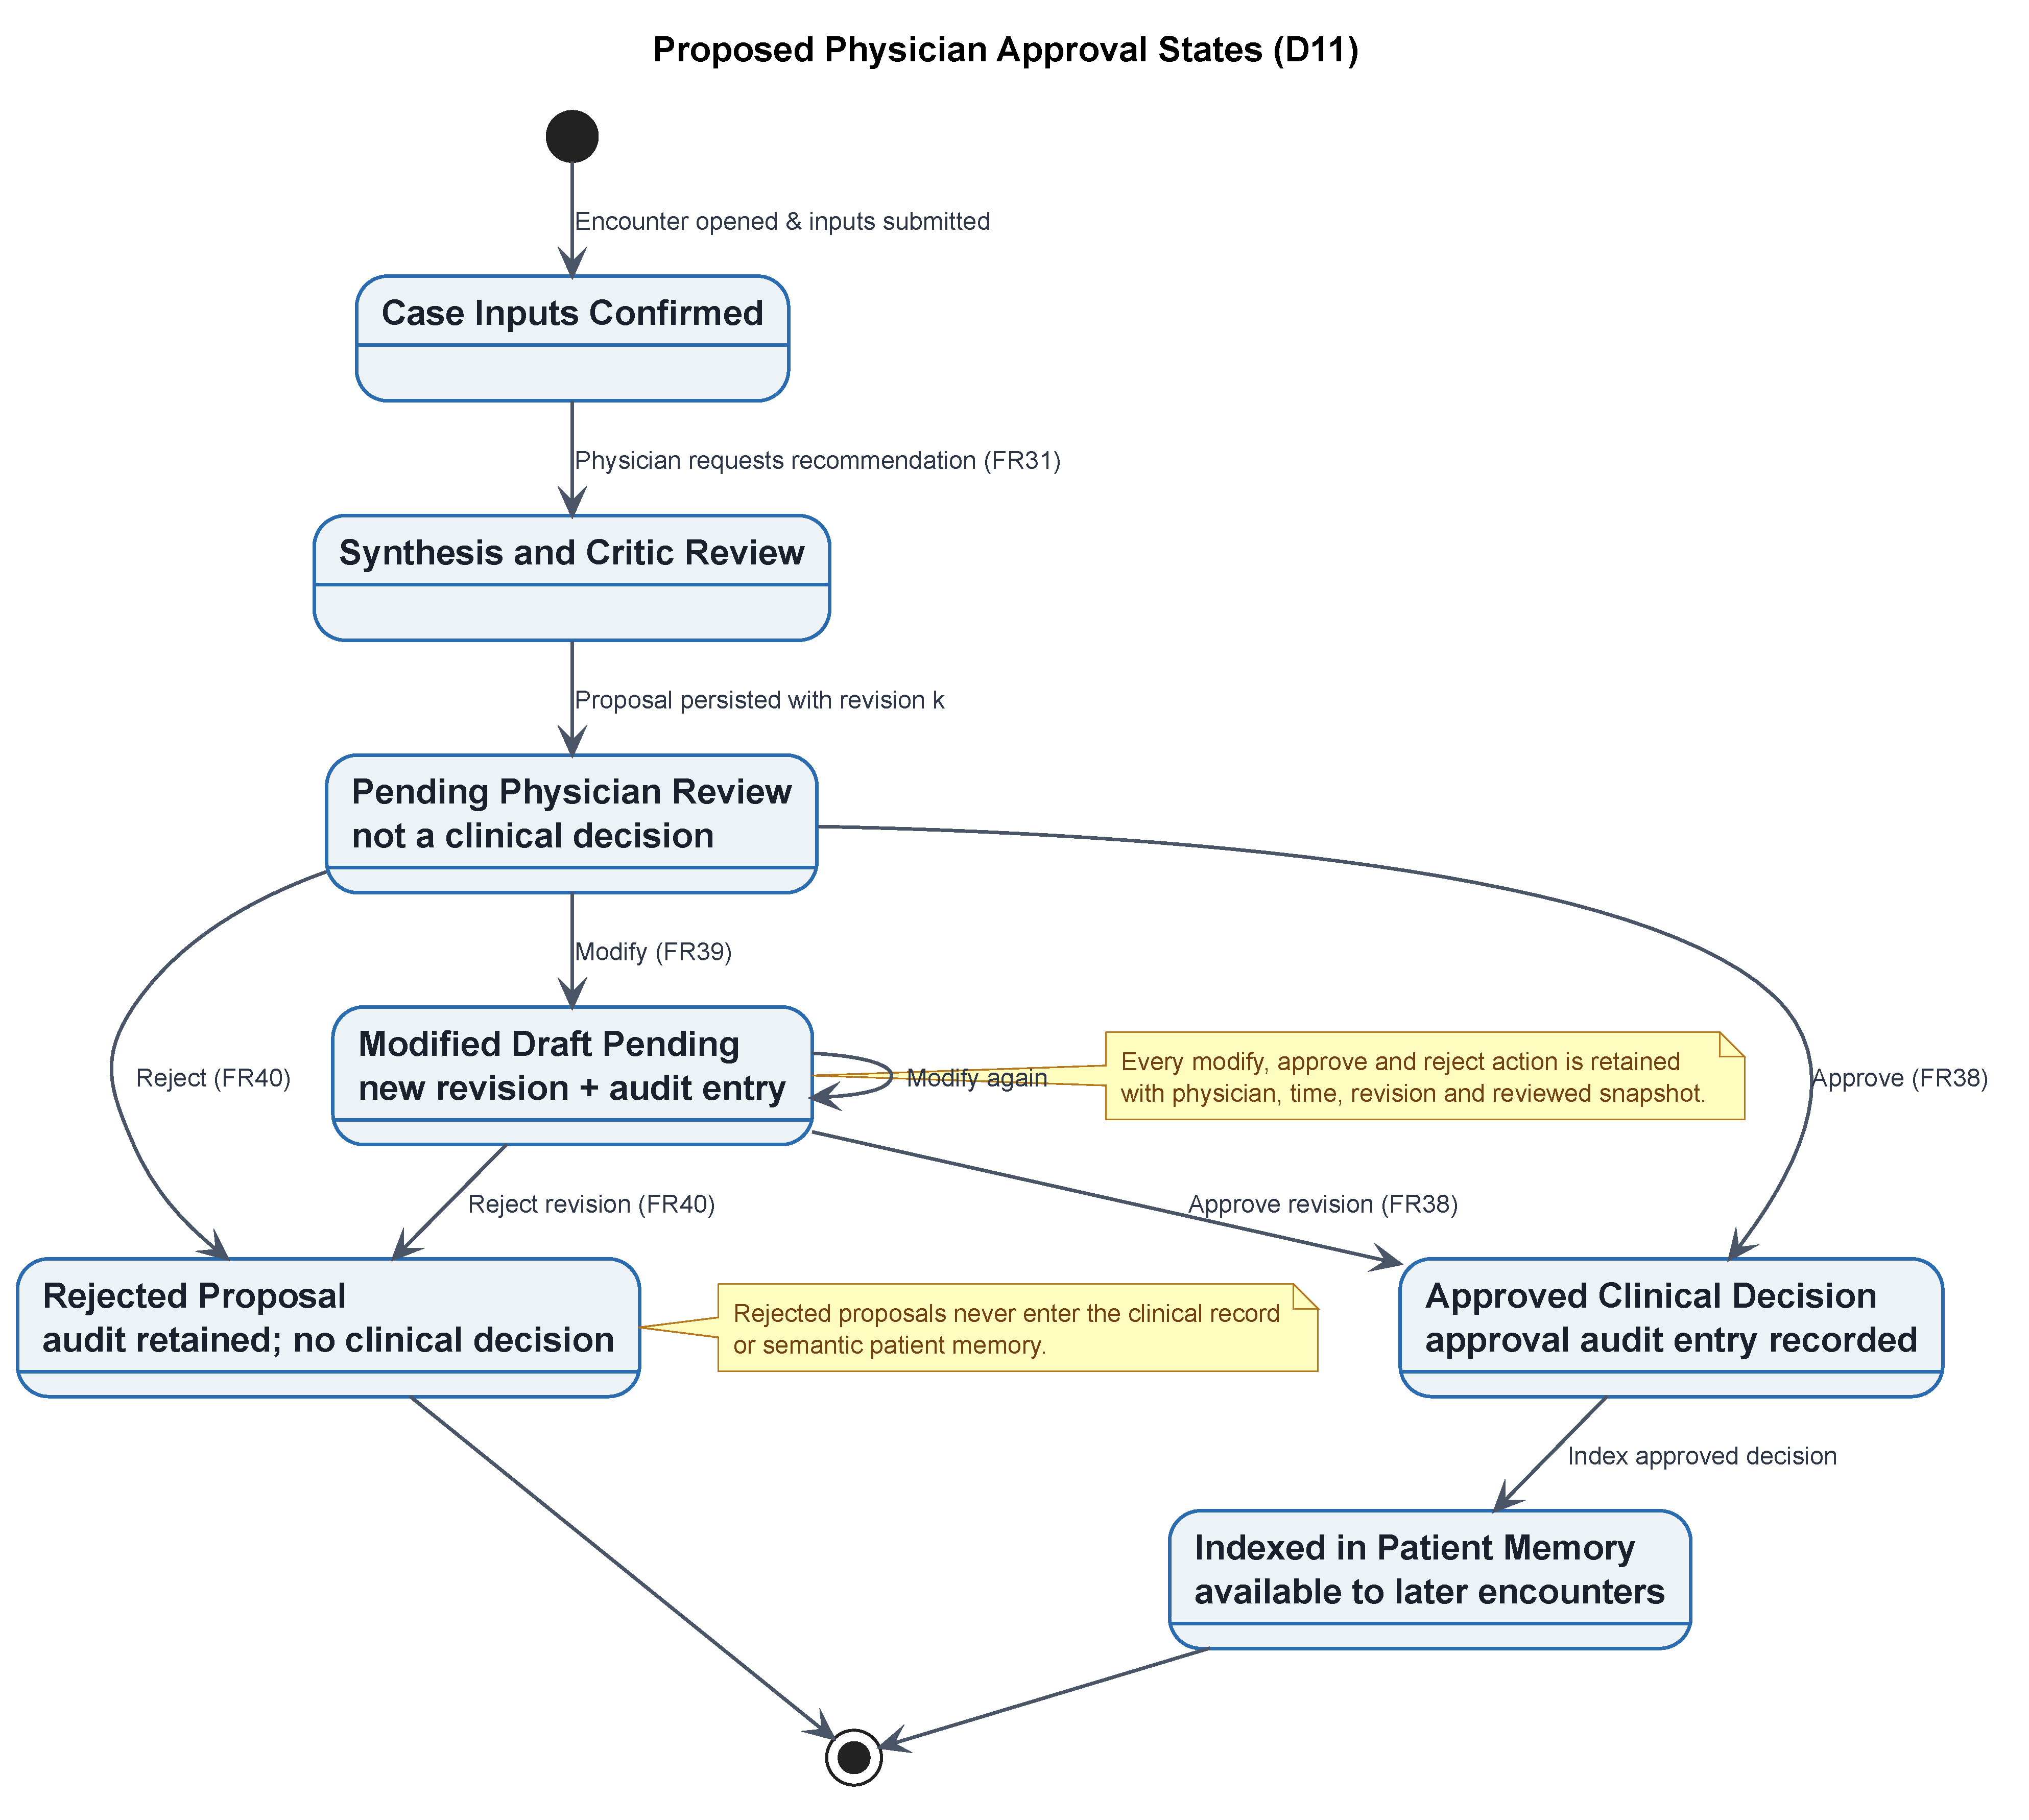
\includegraphics[width=0.88\textwidth,height=0.76\textheight,keepaspectratio]{Figures/esha_D11_approval_states.pdf}
\caption{Physician-controlled draft states and explicit approval transitions.}
\label{fig:esha:d11}
\end{figure}

\subsection{Grounded Clinical Evidence Citation and Critic Verification Tactic}

The Evidence and RAG Agent returns supporting passages with source identifiers and citations rather than only an explanation. The Clinical Reasoning Agent uses these passages alongside patient context and specialist findings when preparing a diagnosis and treatment draft. Evidence links identify the saved revision they support, allowing the physician to inspect the relationship between a recommendation and its sources. The Safety and Critic Agent examines the draft for insufficient support, inconsistency and safety concerns before presentation. Critic findings retain their assessed revision and appear alongside the draft, including concerns that remain unresolved. Missing evidence must be shown as missing rather than replaced with fabricated citations, and critic review must not be described as proof of correctness. Physician approval remains necessary regardless of the critic outcome. These tactics complete the architecture's review pathway and establish comparison targets for evidence support and critic contribution; their effectiveness requires implemented workflows and measured evaluation.

\section{Conclusion}

The design translates Zeest's requirements into a physician interface, application gateway, coordinated agents, supporting analytical services and hybrid memory. Defined boundaries preserve patient ownership and distinguish source observations, specialist findings, generated drafts and accepted decisions. Revision relationships connect the information used for analysis with the evidence and critic findings presented during review. Application services govern approval and audit recording, while analytical agents remain responsible for preparation, retrieval and recommendations. The domain model and behavioural diagrams provide complementary views of these responsibilities and their permitted transitions. Component adapters and visible failure states support integration without implying that every candidate resource is already available. The architecture also accommodates controlled research comparisons by retaining case definitions, configurations and outputs independently of clinical decision records. Implementation must validate these contracts, transaction boundaries and failure paths before performance or clinical-value claims can be made. The resulting design provides a coherent development foundation while preserving physician authority and the limits of the current research scope.

\endgroup
%
{
\bibliographystyle{ieeetr}
\bibliography{../kashaf/references,../fatima/references,../esha/references} %specify your .bib file here
}
%ADD APPENDICES IF REQUIRED OTHERWISE COMMENT IT OUT
\appendix
% Owner: Kashaf Ali / Member A. Approved final integration.
\chapter{Traceability and Design Decisions}

The supplementary tables consolidate the relationships between Zeest's objectives, clinical workflow and intended verification activities. They distinguish implementation checks from comparative research so that a requirement is not considered satisfied merely because a diagram or interface design exists. Patient ownership applies throughout clinical work, input and draft revisions preserve source content, and explicit approval determines which reviewed content becomes a clinical decision. Comparative evaluation uses permitted cases and recorded configurations, with the same reference procedure applied across variants. Candidate datasets, models and knowledge resources require selection and permission checks before use. The design provides no measured outcomes, dataset-access guarantee or claim of clinical deployment. Configuration-dependent values therefore remain identified decisions rather than invented numbers. The tables support implementation and assessment while preserving the distinction between source observations, generated recommendations and accepted decisions. They also connect changes to requirements with the corresponding methodology and architecture responsibilities established across the six chapters.

\section{Objective Traceability}
Table~\ref{tab:kashaf:appendix-trace} connects the nine objectives with their requirements and intended verification.

\begin{table}[htbp]
\centering
\small
\caption{Objectives, requirement locations and intended verification.}
\label{tab:kashaf:appendix-trace}
\begin{tabular}{|p{0.24\textwidth}|p{0.23\textwidth}|p{0.43\textwidth}|}
\hline
Objective & Requirement location & Verification \\ \hline
O1 Hybrid memory & FR23--FR24 & Check patient-scoped relational and semantic retrieval. \\ \hline
O2 Consultation notes & FR14--FR18 & Check capture, transcription and saved corrections. \\ \hline
O3 Specialist agents & FR25--FR30 & Check source-aware findings and stage failures. \\ \hline
O4 Existing imaging model & FR19, FR26 & Check supported inputs against the selected model. \\ \hline
O5 Cited evidence & FR32, FR36 & Assess retrieved source relevance and passage support. \\ \hline
O6 Clinical draft & FR31, FR33--FR34 & Assess diagnosis and treatment drafts against reference cases. \\ \hline
O7 Critic review & FR35, FR37 & Compare concerns and outputs with and without critic review. \\ \hline
O8 Physician control & FR38--FR44 & Check revision-specific actions, decisions and audit records. \\ \hline
O9 Comparative evaluation & RR01--RR04 & Compare the baseline, memory variant and full system under common conditions. \\ \hline
\end{tabular}
\end{table}
\clearpage
\section{Configuration Decisions}
Table~\ref{tab:kashaf:appendix-decisions} separates established boundaries from choices required before execution.

\begin{table}[htbp]
\centering
\small
\caption{Established design boundaries and outstanding execution choices.}
\label{tab:kashaf:appendix-decisions}
\begin{tabular}{|p{0.26\textwidth}|p{0.64\textwidth}|}
\hline
Item & Decision or required selection \\ \hline
Patient access & One responsible physician per patient; ownership checks on all clinical operations. \\ \hline
Clinical decision & Explicit approval of the exact saved draft revision; modification alone is not approval. \\ \hline
Memory sources & Authorised input revisions or approved decisions; pending drafts are not accepted facts. \\ \hline
Data and domain & Select permitted de-identified or synthetic cases with suitable model coverage. \\ \hline
Analytical resources & Select transcription, imaging, embedding and medication resources and record their restrictions. \\ \hline
Evidence & Select a permitted corpus, retrieval configuration and citation-preserving passage representation. \\ \hline
Orchestration & Document the LangGraph and Google ADK responsibility split. \\ \hline
Evaluation & Define case count, reference judgements, rubric, workload and thresholds before executing comparisons. \\ \hline
\end{tabular}
\end{table}
%
\end{document}
